%!TEX TS-program = pdflatex
% dissertation.tex -- main dissertation file
%
% Wisconsin dissertation template
% Copyright (c) 2008-2009 William C. Benton.  All rights reserved.
%
% This program can redistributed and/or modified under the terms
% of the LaTeX Project Public License Distributed from CTAN
% archives in directory macros/latex/base/lppl.txt; either
% version 1 of the License, or (at your option) any later version.
%
% This program includes other software that is licensed under the
% terms of the LPPL and the Perl Artistic License; see README for details.
%
% You, the user, still hold the copyright to any document you produce
% with this software (like your dissertation).
%

%%% You'll want ``oneside'' for the deposit version, but probably not for any versions that don't need to meet the UW requirements
\documentclass[12pt,oneside,letterpaper]{memoir}

\usepackage{amsmath}
\usepackage{amssymb}
\usepackage[mathscr]{euscript}
\usepackage{hyperref}
\usepackage{appendix}
\usepackage{algorithm}
\usepackage{algpseudocode}

\newcommand{\norm}[1]{\left\lVert#1\right\rVert}

%--------------------DATA----------------------

% Total number of human, RNA-seq experiments in the SRA
\newcommand{\NumSRAExperiments}{185,000}
% Total number of human samples in the SRA on which RNA-seq was performed
\newcommand{\NumSRASamples}{166,000}
% Total number of studies storing human RNA-seq samples
\newcommand{\NumSRAStudies}{4,500}

% Lower bound of number of biological samples in SRA (in millions)
\newcommand{\SamplesInSRA}{1.5}
% Lower bound of number of studies in SRA 
\newcommand{\StudiesInSRA}{75,000}
% Total human RNA-seq, ILLUMINA samples that we are considering
\newcommand{\TotalSamplesConsidered}{75038}
% Number of samples with non-empty key-value pairs of samples we are considering
\newcommand{\TotalSamplesConsideredNonEmptyKeyVals}{73407}
% Number of distinct studies represented in our considered samples
\newcommand{\DistinctStudiesConsidered}{2681}
% Number of studies with at least 100 samples
\newcommand{\NumberOfLargeStudies}{88}
% Number of studies with less than 100 samples
\newcommand{\NumberOfSmallStudies}{2593}
% Percentage of samples belonging to "large" studies
\newcommand{\PercentageSamplesInLargeStudies}{57}
% Size of training set used to train sample-type classifier
\newcommand{\SampleTypeTrainingSetSize}{705}
% Size of initial test set used to evaluate ontology mapping pipeline and recall for sample-type classifier
\newcommand{\TestSetSize}{422}
% Size of test set of 422 samples considering only those with real-value properties
\newcommand{\TestSetRealValSize}{104}
% Precision and recall on extracting real-value properties
\newcommand{\RealValPrecision}{0.989}
\newcommand{\RealValRecall}{0.672}
% Number of samples in non-enriched test set that could manually annotated with sample-type
\newcommand{\NonEnrichedSampleTypeTestSetSize}{367}
% Accuracy of sample-type classifier over the non-enriched test set (i.e. test set used for evaluating ontology term mapping)
\newcommand{\SampleTypeOverallAccuracy}{0.845}
% Number of samples in the enriched test set used to compute the transpose of the column normalized confusion matrix
\newcommand{\EnrichedSampleTypeTestSetSize}{554}
% Percentage of MetaSRA samples annotated with real-value property
\newcommand{\PercentageMetaSRARealVal}{23.2}


% Total number of bulk primary cell samples
\newcommand{\ExperimentsInBulkDataset}{4,170}
% Number of bulk samples in the bulk training set
\newcommand{\ExperimentsInBulkTrainingDataset}{3,482}
% Total number of studies in the bulk dataset
\newcommand{\StudiesInBulkDataset}{263}
% Total number of cell types in the bulk dataset
\newcommand{\CellTypesInBulkDataset}{297}
% Number of studies in the bulk training set
\newcommand{\StudiesInBulkTrainingDataset}{206}
\newcommand{\ExperimentsInBulkTestDataset}{688}
\newcommand{\StudiesInBulkTestDataset}{57}
\newcommand{\NumCellTypesIntersectTrainingTest}{200}
\newcommand{\MostSpecificBulkCellTypes}{104}
\newcommand{\TrainingSizeURSA}{approximately 9,000}
\newcommand{\ExperimentsInSingleCellDataset}{7,402}
\newcommand{\TotalExperiments}{11,572}
\newcommand{\StudiesInSingleCellDataset}{15}
\newcommand{\CellTypesInSingleCellDataset}{125}
\newcommand{\BulkRestrictedSingleCellExperiments}{4,961} \newcommand{\BulkRestrictedSingleCellStudies}{13}  \newcommand{\BulkRestrictedSingleCellCellTypes}{66}
\newcommand{\RawGenomicFeatures}{200,401}
\newcommand{\GeneLevelFeatures}{58,243}
\newcommand{\DataDownloadURL}{http://deweylab.biostat.wisc.edu/cell\_type\_classification}
\newcommand{\ClassifierURL}{https://github.com/deweylab/CellO}
\newcommand{\CodeURL}{https://github.com/deweylab/cell-type-classification-paper}

\newcommand{\FracEdgesInconsistent}{6.9\%}
\newcommand{\EdgesSeverelyInconsistent}{32}
\newcommand{\MinGenesInGOSet}{5}

\newcommand{\NumTenXGenes}{32,738}
\newcommand{\NumTenXIntersection}{31,283}

%----------------------------------------------


\input{includes/preamble}
\input{includes/defs}
\input{includes/thesisdefs}
\svnidlong{$LastChangedBy$}{$LastChangedRevision$}{$LastChangedDate$}{$HeadURL: http://freevariable.com/dissertation/branches/diss-template/dissertation.tex $} 

\clearpage\pagenumbering{roman}  % This makes the page numbers Roman (i, ii, etc)

\title{Computational methods for transcriptome-based cellular phenotyping}
\author{Matthew N. Bernstein}
\department{Computer Sciences}

\date{2019}

\begin{document}

%%% Uncomment the following if your .bib contains references that you will not 
%%% explicitly cite, but that should be in the final bibliography:
% \nocite{*}

\ifpdf
\DeclareGraphicsExtensions{.pdf, .jpg, .tif}
\else
\DeclareGraphicsExtensions{.eps, .jpg}
\fi

\maketitle

%% Add \part declarations if you want, but it's not necessary
%\part{Preliminaries}

\svnidlong{$LastChangedBy$}{$LastChangedRevision$}{$LastChangedDate$}{$HeadURL: http://freevariable.com/dissertation/branches/diss-template/frontmatter/frontmatter.tex $}
\vcinfo{}

%%% SOME OF THIS CODE IS ADAPTED FROM THE VENERABLE withesis.cls

% COPYRIGHT PAGE
%  - To include a copyright page use \copyrightpage
\copyrightpage

% DEDICATION
\begin{dedication}
	\emph{To my parents.}
\end{dedication}

%% BEGIN PAGESTYLE

%%% You can pick a pagestyle if you want; see the memoir class
%%% documentation for more info.  The default ``deposit'' option meets
%%% the UW thesis typesetting requirements but is probably
%%% unsatisfactory for making a version of your dissertation that
%%% won't be deposited to the graduate school (e.g. for web or a nice
%%% printed copy)

\chapterstyle{deposit}
\pagestyle{deposit}


% ACKNOWLEDGMENTS
\begin{acks}
First, I would like to thank my advisor, Colin Dewey, for his kind and dedicated mentorship over the years and for teaching me how to conduct rigorous and insightful science.  I have immensely enjoyed these years learning from and working with him. His kindness and dedication has set for me a strong example of academic mentorship.  I would also like to thank my committee for their valuable guidance. I thank AnHai Doan for providing me direction in the early stages of the MetaSRA project in showing me how to iteratively develop the MetaSRA pipeline in a data-driven manner.  I wish to thank Mark Craven for not only serving on my committee, but also for teaching my first machine learning course during my first semester at UW-Madison, which helped to ignite my passion for this field. I thank Matt Ziegler for his help in building a fantastic interface for the MetaSRA website.  I am also indebted to the Computation and Informatics in Biology and Medicine training program for funding three years of my PhD and for providing me abundant opportunities to present my work. 

Earning a PhD is never an individual's accomplishment.  Rather, it requires a strong network of love and support, which I am extremely grateful to have had. First, I would like to thank my parents for their unconditional love and unwavering support throughout my entire life which made everything I have accomplished possible. To my brothers David and Max for their lifelong friendship, and those enjoyable late night conversations on topics both silly and serious. To Hannah for her love, for lifting me up during the hard times, and for pushing me to be the best person I can be.  To my Madison friends Shoban Chandrabose, Stephen Brown, Steve Lazzaro, Isaac Harrington, Marissa Gaskill, Shree Hardikar, Alisa Maas, Ross Kleiman, Alexi Brooks, and others who have helped me stay balanced - from board game nights to Comedy Club outings, nights on the Terrace to corn mazes. And lastly, a quick shout-out to the furry companionship of Duke, Korra, Taco, and Beeb.  Thank you all.
\end{acks}

% CONTENTS, TABLES, FIGURES
\renewcommand{\printtoctitle}[1]{\chapter*{#1}}
\renewcommand{\printloftitle}[1]{\chapter*{#1}}
\renewcommand{\printlottitle}[1]{\chapter*{#1}}

\renewcommand{\tocmark}{}
\renewcommand{\lofmark}{}
\renewcommand{\lotmark}{}

\renewcommand{\tocheadstart}{}
\renewcommand{\lofheadstart}{}
\renewcommand{\lotheadstart}{}

\renewcommand{\aftertoctitle}{}
\renewcommand{\afterloftitle}{}
\renewcommand{\afterlottitle}{}

\renewcommand{\cftchapterfont}{\normalfont} 
\renewcommand{\cftsectionfont}{\itshape} 
\renewcommand{\cftchapterpagefont}{\normalfont} 
\renewcommand{\cftchapterpresnum}{\bfseries} 
\renewcommand{\cftchapterleader}{} 
\renewcommand{\cftsectionleader}{} 
\renewcommand{\cftchapterafterpnum}{\cftparfillskip} 
\renewcommand{\cftsectionafterpnum}{\cftparfillskip} 

% \captionnamefont{\small\sffamily} 
% \captiontitlefont{\small\sffamily} 

% \renewcommand{\contentsname}{contents}
% \renewcommand{\listfigurename}{list of figures}
% \renewcommand{\listtablename}{list of tables}

\tableofcontents

\clearpage
\listoftables

\clearpage
\listoffigures

\clearpage
% NOMENCLATURE
% \begin{conventions}
% % \begin{description}
% % \item{\makebox[0.75in][l]{term}
% %        \parbox[t]{5in}{definition\\}}
% % \end{description}
% \input{conventions}
% \end{conventions}

%% The UW graduate school no longer wants a UMI abstract page
%% Should you need one for some reason, uncomment the following
%% lines.  Thanks to Matt Fredrikson for reporting this!

% \advisorname{Gottlob Frege}
% \advisortitle{Professor}
% \begin{umiabstract}
%  Although the basic chemical mechanisms of cellular biology are now well-known, we are still a long way from understanding how phenotypes emerge from these basic mechanisms. Within the last decade, RNA-sequencing (RNA-seq) has become a ubiquitous technology for measuring the transcriptome, which provides a snapshot of gene expression across the entire genome.  An improvement in our ability to predict how phenotypes emerge from the complex patterns of gene expression, a task we refer to as \textit{transcriptome-based cellular phenotyping} (TBCP), would lead to considerable medical and technological advancements.  Machine learning promises to be an apt approach for TBCP due to its ability to overcome noise inherent in RNA-seq data and because it does not require a priori knowledge regarding the rules and patterns that lead from gene expression to phenotype. Furthermore, there exist large, public databases of RNA-seq data that promise to be a valuable source of training data for developing machine learning algorithms to perform TBCP.  Unfortunately, this opportunity is impeded by a number of challenges inherent in these databases including poorly structured metadata and data heterogeneity.  In this thesis, I present three projects that push the state-of-the-art in the ability to leverage the trove of publicly available gene expression data for TBCP. 

In the first project, we address the problem of poorly structured metadata that exist in public genomics databases. We specifically focus on the Sequence Read Archive (SRA), which is the premiere repository of raw RNA-seq data curated by the National Institutes of Health; however, our work generalizes to other databases.  Existing approaches treat metadata normalization as a named entity recognition problem where the goal is to tag metadata with terms from controlled vocabularies when that term is mentioned in the metadata. We reframe this problem as an inference task, in which we tag the metadata with only those terms that describe the underlying biology of the described sample rather than with all mentioned terms. By doing so, we achieve higher precision than that achieved by existing methods, and maintain a competitive recall.
 
In the second project, we leverage the normalized metadata produced by the first project in order to train predictive models of phenotype from RNA-seq derived gene expression data. We specifically focus on the cell type prediction task: given an RNA-seq sample, we wish to predict the cell type from which the sample was derived.  Cell type prediction is an important step in many transcriptomic analyses, including that of annotating cell types in single-cell RNA-seq datasets. This work represents the first effort towards a cell type prediction task that utilizes the full potential of publicly available RNA-seq data.  
 
 Finally, in the third project, we build on the second project in order to address the task of cell type prediction on \textit{sparse} single-cell RNA-seq data (scRNA-seq) produced by novel droplet-based technologies.  These droplet-based scRNA-seq technologies are enabling the sequencing of higher numbers of cells at the cost of a lower read-depth per cell. Such low read-depths result in fewer genes with detected expression per cell.  We explore the effects of applying cell type classifiers trained on dense, bulk RNA-seq data to sparse scRNA-seq data and propose a novel probabilistic generative model for adapting the bulk-trained classifiers to sparse input data.



% \end{umiabstract}

\begin{abstract}
  Although the basic chemical mechanisms of cellular biology are now well-known, we are still a long way from understanding how phenotypes emerge from these basic mechanisms. Within the last decade, RNA-sequencing (RNA-seq) has become a ubiquitous technology for measuring the transcriptome, which provides a snapshot of gene expression across the entire genome.  An improvement in our ability to predict how phenotypes emerge from the complex patterns of gene expression, a task we refer to as \textit{transcriptome-based cellular phenotyping} (TBCP), would lead to considerable medical and technological advancements.  Machine learning promises to be an apt approach for TBCP due to its ability to overcome noise inherent in RNA-seq data and because it does not require a priori knowledge regarding the rules and patterns that lead from gene expression to phenotype. Furthermore, there exist large, public databases of RNA-seq data that promise to be a valuable source of training data for developing machine learning algorithms to perform TBCP.  Unfortunately, this opportunity is impeded by a number of challenges inherent in these databases including poorly structured metadata and data heterogeneity.  In this thesis, I present three projects that push the state-of-the-art in the ability to leverage the trove of publicly available gene expression data for TBCP. 

In the first project, we address the problem of poorly structured metadata that exist in public genomics databases. We specifically focus on the Sequence Read Archive (SRA), which is the premiere repository of raw RNA-seq data curated by the National Institutes of Health; however, our work generalizes to other databases.  Existing approaches treat metadata normalization as a named entity recognition problem where the goal is to tag metadata with terms from controlled vocabularies when that term is mentioned in the metadata. We reframe this problem as an inference task, in which we tag the metadata with only those terms that describe the underlying biology of the described sample rather than with all mentioned terms. By doing so, we achieve higher precision than that achieved by existing methods, and maintain a competitive recall.
 
In the second project, we leverage the normalized metadata produced by the first project in order to train predictive models of phenotype from RNA-seq derived gene expression data. We specifically focus on the cell type prediction task: given an RNA-seq sample, we wish to predict the cell type from which the sample was derived.  Cell type prediction is an important step in many transcriptomic analyses, including that of annotating cell types in single-cell RNA-seq datasets. This work represents the first effort towards a cell type prediction task that utilizes the full potential of publicly available RNA-seq data.  
 
 Finally, in the third project, we build on the second project in order to address the task of cell type prediction on \textit{sparse} single-cell RNA-seq data (scRNA-seq) produced by novel droplet-based technologies.  These droplet-based scRNA-seq technologies are enabling the sequencing of higher numbers of cells at the cost of a lower read-depth per cell. Such low read-depths result in fewer genes with detected expression per cell.  We explore the effects of applying cell type classifiers trained on dense, bulk RNA-seq data to sparse scRNA-seq data and propose a novel probabilistic generative model for adapting the bulk-trained classifiers to sparse input data.



\end{abstract}

\clearpage\pagenumbering{arabic}

%%% END STUFF TAKEN FROM WITHESIS EXAMPLE FILE


%% Now include the tex files for each chapter, like so (I put these in separate dirs): 
\chapter{Introduction} \label{chap:intro}

Although the basic chemical mechanisms of cellular biology are now well-known, we are still a long way from understanding how most observable characteristics of a cell or organism -- called \textit{phenotypes} -- emerge from these basic mechanisms. Advances within the last decades are now enabling high-dimensional measurements of cells, thereby allowing us to study this emergent complexity.  For example, within the last decade, RNA-sequencing (RNA-seq) has become a ubiquitous technology for measuring the set of all RNA gene products in a cell or biological sample -- called the \textit{transcriptome} -- thereby providing a snapshot of the gene activity across the entire genome (\citealp{Wang2009}).  An improvement in our ability to predict how phenotypes emerge from the complex patterns of gene activation, as captured by RNA-seq, would lead to considerable medical and technological advancements in such areas as stem cell therapy development (\citealp{Cahan, Morris2014}), disease diagnosis (\citealp{Kegerreis2019, Bryon2016, Saddiki2015, Marisa2013, Chuang2007}), and biological data analysis (\citealp{Hou2019, Alavi2018, Ellis}).  This task, which we refer to as \textit{transcriptome-based cellular phenotyping} (TBCP), is the focus of this dissertation.

Currently, it remains intractable to perform TBCP manually due to both the high number of genes (tens of thousands in the human genome) and our incomplete understanding of how the myriads of interactions between genes, proteins, and other molecules in the cell form complex systems and feedback loops.  Thus, computational approaches are required. Furthermore, biological systems are inherently noisy, so these computational approaches must take this noise into account if they are to be successful. In this dissertation, we explore the use of \textit{machine learning} --  the study of algorithms that learn by example -- for building automated TBCP systems.  Machine learning is an apt approach for overcoming the noise inherent in RNA-seq data because incorporating uncertainty is fundamental to machine learning algorithms (\citealp{Ghahramani2015}).  Furthermore, since machine learning algorithms learn from examples, these approaches provide a path to overcoming the lack of knowledge regarding the specific rules and patterns that lead from gene activity to phenotype. 
 
Although machine learning algorithms do not require a priori knowledge, they do require training examples.  In the case of applying machine learning to TBCP with RNA-seq, this entails providing the algorithm with RNA-seq data from many biological samples where each sample is labelled with a phenotype.  Unfortunately, it remains difficult for a single laboratory to produce sufficient data to train such algorithms because sample collection, preparation, and RNA-sequencing are expensive and involved processes. Fortunately, the National Institutes of Health (NIH) have created public databases where scientists who perform RNA-seq deposit their data so that other scientists can perform secondary analyses. These databases thus provide a valuable source of training data for the TBCP task.

Unfortunately, it has hitherto been challenging to utilize these public data sources due to their poorly structured metadata and heterogeneity.  In this dissertation we present three projects that address these challenges and span multiple stages of the machine learning pipeline, from the acquisition of training data to model development. These projects support the following thesis:
\begin{quote}
Large-scale, heterogeneous repositories of RNA-seq data can be leveraged to train machine learning classifiers to perform transcriptome-based cellular phenotyping.
\end{quote}
Most of this work targets the Sequence Read Archive (SRA), the premier repository of public RNA-seq data, which is curated by the NIH (\citealp{Leinonen2011}); however, this work may also be applied to other large, related databases including the Gene Expression Omnibus (\citealp{Barrett2013}).  Together, these projects advance the state-of-the-art in both our ability to leverage public data and to perform TBCP. 

In the following sections, we provide relevant background on RNA-seq, applications of TBCP, and relevant computational approaches.  The purpose of this introduction is to bridge the gap between computer scientists, biologists, and bioinformaticians.



\section{Transcriptomic analysis with RNA-seq}

Each cell in an organism contains a copy of its genome: a long sequence of four molecules, adenine (A), thymine (T), guanine (G), and cytosine (C), called DNA.  Specific subsequences along the genome are called \textit{genes} and store the instructions for constructing functional molecules, predominantly \textit{proteins}, that orchestrate the cell's chemistry\footnote{The human genome encodes approximately 20,000 protein-coding genes.}. When a gene is \textit{expressed} by the cell (i.e. used to create a protein), the gene's sequence is first copied to an intermediate information-storing molecule, called RNA, in a process called \textit{transcription} . These RNA molecules, called \textit{transcripts}, are free to float away from the DNA where they bind with cellular machinery, called \textit{ribosomes}, which are responsible for converting the transcript's sequence into a protein\footnote{Some genes do not encode for a protein. Rather, the RNA itself performs a function in the cell. These RNA are often called \textit{non-coding RNA's}.}.  The set of all transcripts in the cell is called the \textit{transcriptome}.

RNA-seq is a procedure that leverages next-generation sequencing of DNA molecules in order to measure the relative abundance of each gene's transcripts in the cell (Fig.~\ref{fig:rna_seq_protocol}). The procedure works as follows: first, RNA is isolated from the cell or population of cells. The isolated RNA is then broken into fragments, reverse transcribed into DNA, and then amplified thereby creating a set of short DNA molecules called the \textit{sequencing library}. The sequencing library is then fed to a next-generation sequencing machine where the DNA fragments are sampled uniformly at random, and a short substring is read off of the ends of these sampled fragments.  These substrings, called \textit{reads}, are then stored in a digital file\footnote{A typical RNA-seq experiment will produce a file storing tens of millions of reads. These files typically occupy several gigabytes.}.  By design, each step of the RNA-seq protocol preserves, on average, the relative proportion of transcript copies from each gene. Thus, by examining the proportion of reads originating from each gene one can infer the expression level of that gene.  

Determining the gene of origin for each read is a challenging computational problem. Classical approaches entail \textit{aligning} the reads to the genome -- that is, finding the best character-to-character match between the read and a subsequence along the genome (\citealp{Canzar2017}).  Recent approaches bypass the explicit character-by-character alignment process and instead compute approximate alignments, referred to as either \textit{pseudoalignments} (\citealp{Bray2016}) or \textit{quasi-mappings} (\citealp{Patro2017}).  Once reads are aligned, or approximately aligned, one must deal with reads that map to multiple genomic locations.  Current approaches treat this multi-mapping read assignment problem as an inference task where the goal is to infer the true gene of origin for reach read (\citealp{Li2011, Li2010}).  The final output is a positive, real number associated with each gene indicating the estimated, expected number of reads that originate from each gene.  Mathematically, one can represent this output as a vector of read-counts, $\bold{x} \in \mathbb{R}^G$, where $G$ is the number of genes, and an element of this vector $x_i$ represents the number of reads mapping to gene $i$.

%This read alignment problem is further challenged by the fact that read alignments must span \textit{intronic} gaps \footnote{Human genes are comprised of two types of regions: exons and introns. Only the exons encode for the protein molecule. After transcription, the introns are "cut" out of the RNA molecule in a process called \textit{splicing}. The remaining RNA sequence is comprised of only exons.} (\citealp{Kim2014, Dobin2012}).  

\begin{figure*}[!tpb]
\centerline{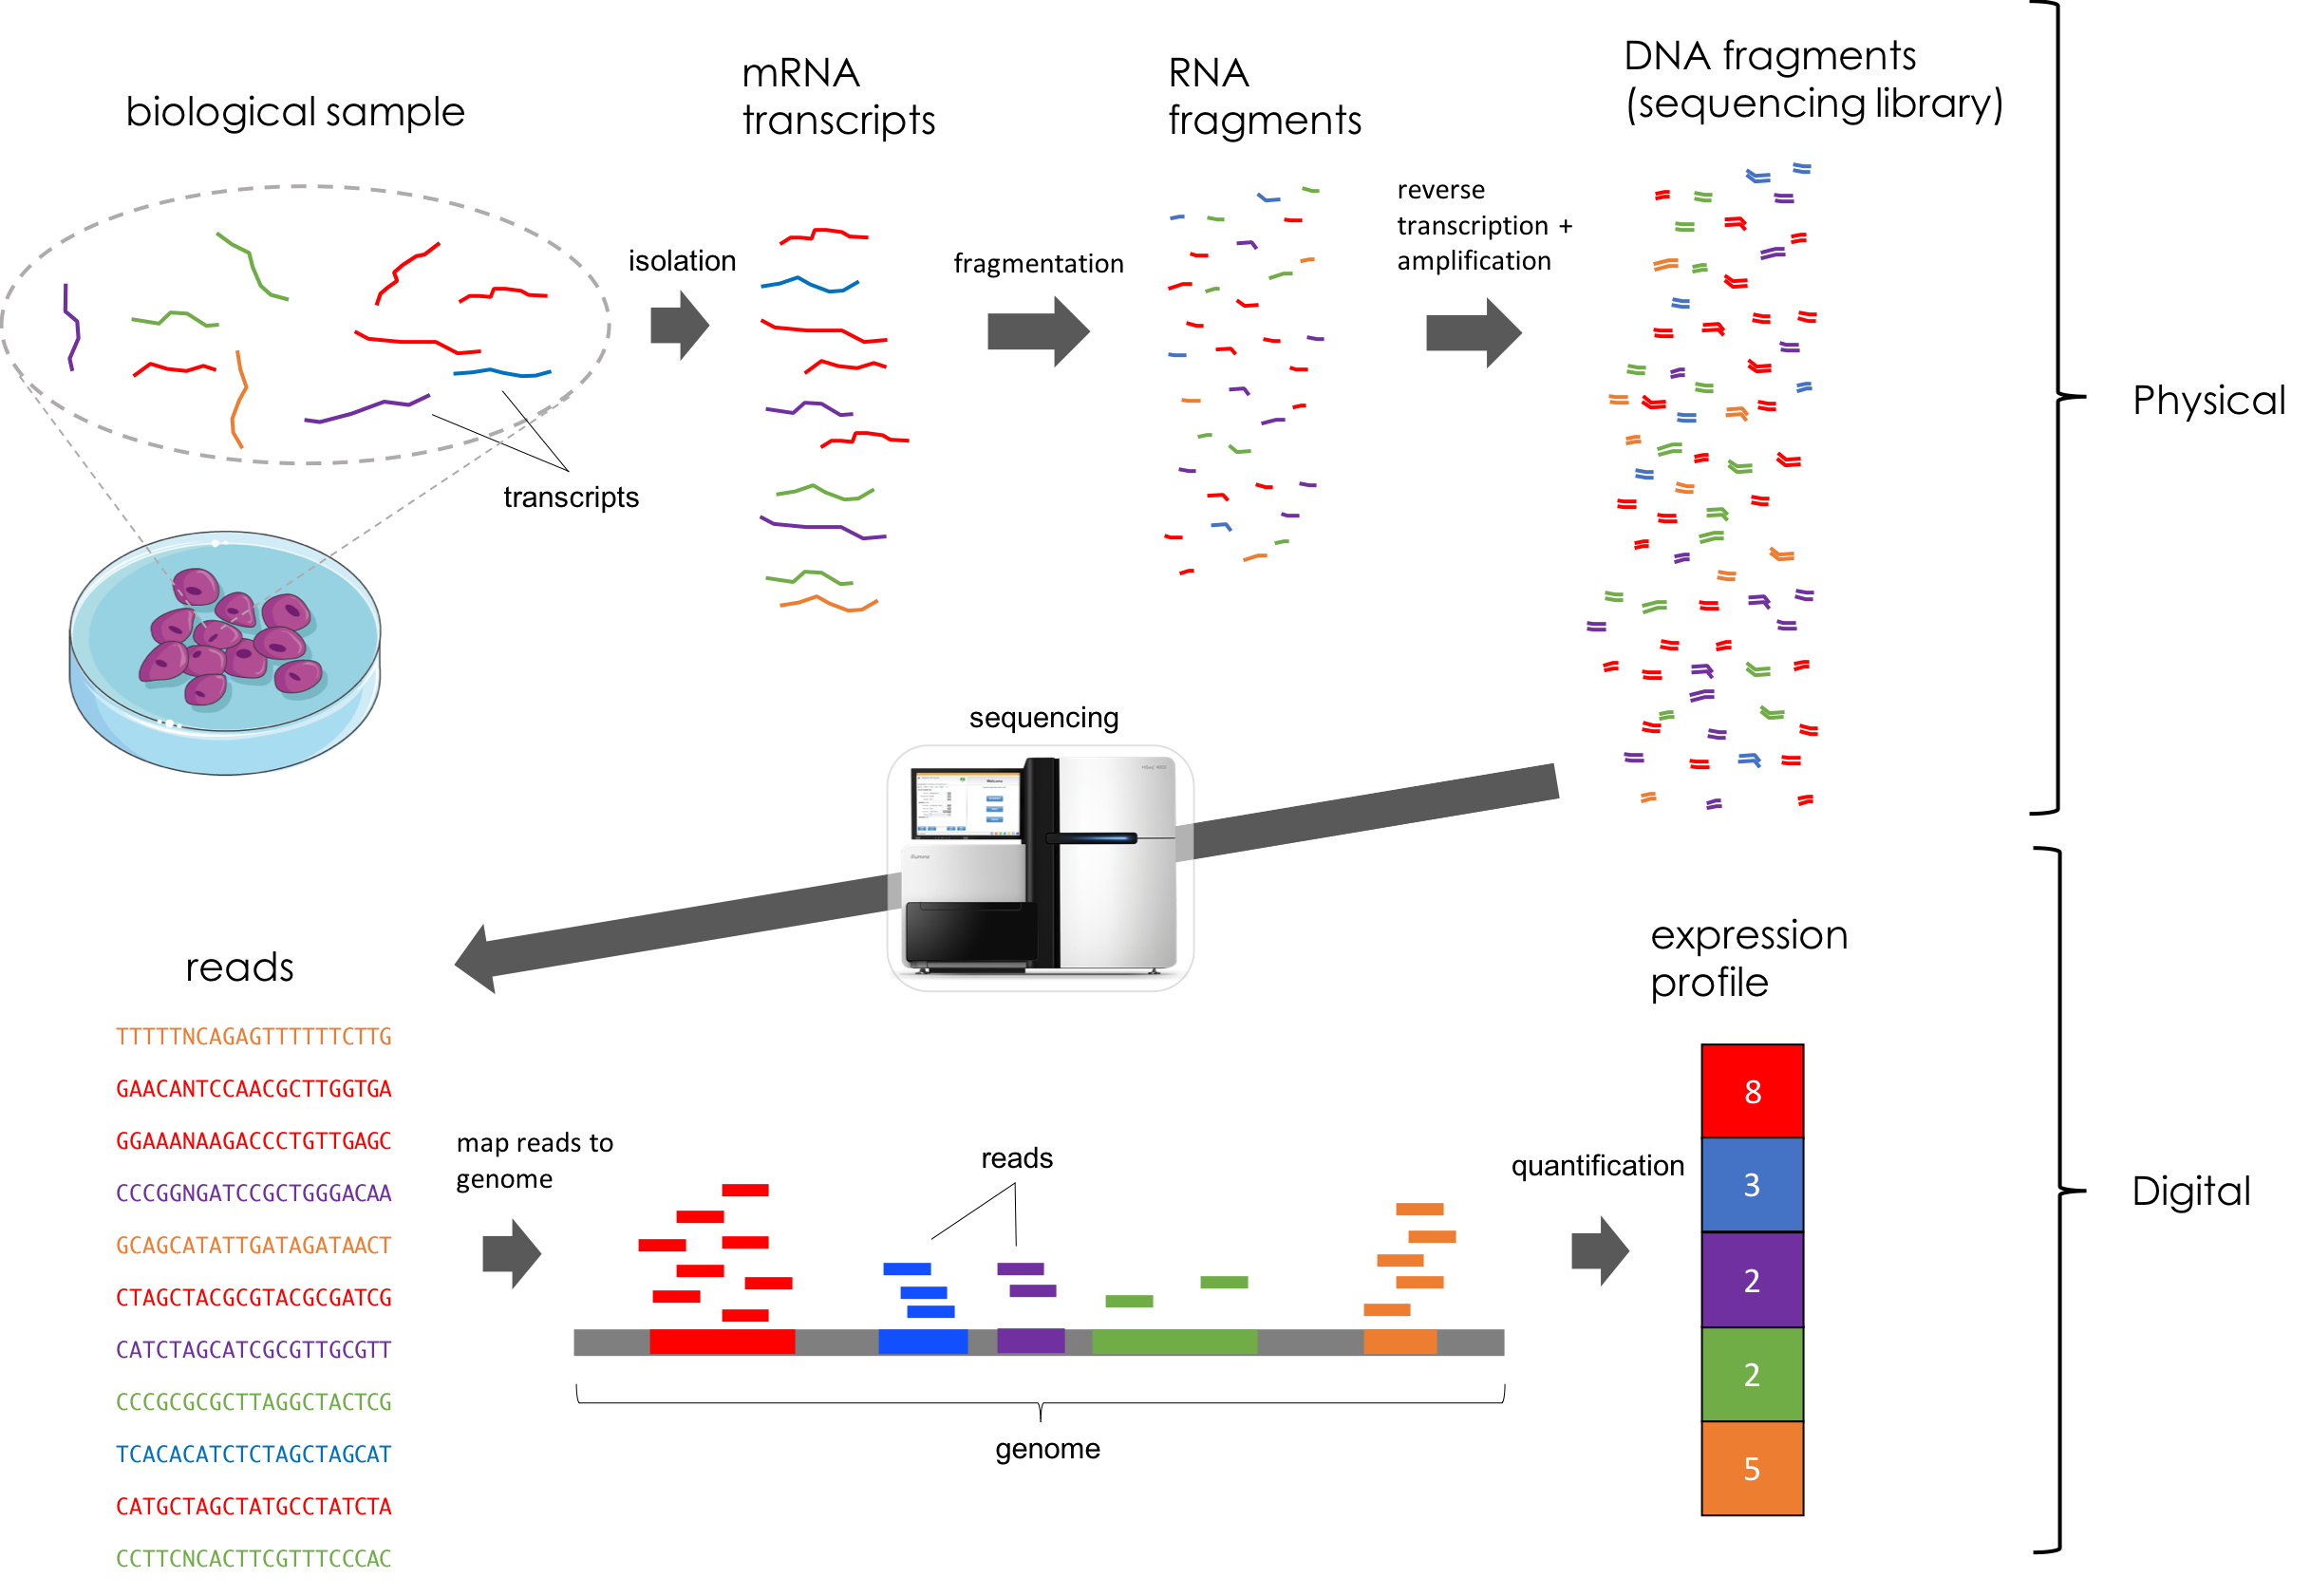
\includegraphics[scale=0.35]{figures/RNA_seq_schematic.png}}
\caption{\textbf{RNA-seq Overview.} A schematic illustrating a basic RNA-seq protocol. In this toy example there are five genes colored red, blue, green, orange, and purple. Each transcript and read is colored according to its gene of origin.}
\label{fig:rna_seq_protocol}
\end{figure*}


\section{Applications of transcriptome-based cellular phenotyping}

TBCP has a number of important applications.  In this section, we discuss some of these applications and notable efforts towards addressing them.

\subsection{Single-cell RNA-seq analysis}

In a traditional RNA-seq experiment, the RNA is isolated and pooled from a population of cells. In these \textit{bulk RNA-seq} experiments, only the average gene expression for the population can be obtained rather than the gene expression of individual cells.   Within the last several years, advances in microfluidics have enabled the development of new protocols, called \textit{single-cell RNA-seq} (scRNA-seq), that entail isolating and extracting RNA from individual cells, thereby allowing for the study of gene expression at the single-cell level (\citealp{Tang2009}).  scRNA-seq enables the study of cell populations at a level of granularity never before accessible, and is therefore leading to discoveries of new cell populations (\citealp{Aizarani2019, Plasschaert2018}) and new mechanisms that account for both healthy tissue function (\citealp{Tikhonova2019, Economo2018}) and disease (\citealp{Mathys2019, Vladoiu2019}).  Furthermore, these technologies are undergoing rapid development and are enabling the sequencing of ever-more cells per experiment. For example, one recent study generated expression profiles for over a hundred thousand cells (\citealp{TabulaMuris2018}).

Scientists who perform scRNA-seq commonly need to identify the cell type of each cell in their dataset.  We consider the task of developing automated systems for classifying cell types in scRNA-seq data to be a TBCP task where cell type is the phenotype of interest.  Traditionally, labeling cell types in scRNA-seq data is an ad hoc process that involves clustering the cells and then searching for differential expression of certain cell-type-specific marker genes across these clusters. This process is challenged both by the fact that there is not a canonical set of marker genes for most cell types (\citealp{Zhang2018}) and that this process is affected by the clustering algorithm (\citealp{Kiselev2019}). To address these issues, approaches are beginning to emerge that rely on training cell type classifiers  (\citealp{Hou2019, Kanter2019, Xie2019, Aran2019, Lieberman2018, Alavi2018, Lin2017}).  

\subsection{Stem cell engineering}

\textit{Stem cells} are a category of cells in multicellular organisms that are capable of converting themselves into more specialized cell types through a process called \textit{differentiation}.  Because of their plasticity, there is great interest in understanding and controlling this differentiation in order to direct cells into becoming a specific targeted tissue type (\citealp{Tewary2018}).  The ability to engineer cells from stem cells is heralding new therapies for regenerating and repairing diseased and injured tissue (\citealp{DeLuca2019}).  

When scientists develop these in vitro differentiation protocols, they must assess how well the differentiated cells resemble the targeted cell type in vivo. To assess this, scientists will often compare a number of characteristics, including gene expression, of their in vitro differentiated cells to fresh, primary cells. To this end, machine learning based TBCP methods have been developed to facilitate this comparison (\citealp{Roost2015, Cahan}).  The idea here is that a machine learning model can classify the cell type or tissue type of the in vitro differentiated cells and the classifier's prediction can inform the user as to what cell type or tissue type the differentiated cells resemble.  The user can then use this knowledge in the diagnoses of their differentiation protocols (\citealp{Morris2014}).
 
\subsection{Disease diagnosis}

Because the transcriptome plays a major role in determining the cell's state, disease processes are often associated with aberrations in the transcriptome.  Therefore, TBCP promises to be a powerful tool for clinical diagnosis (\citealp{Bryon2016}).  For example, in metastasized cancer, a first step in treatment determination is identifying the cancer's tissue of origin. To this end, researchers are exploring machine learning-based TBCP for identifying the tissue of origin in metastasized cancers (\citealp{Sun2018, Li2017}). Along similar lines, researchers are identifying new cancer subtypes, even within the same tissue (\citealp{Hoadley2018}). As the landscape of cancer subtypes is further revealed, new TBCP tools will be required to classify the subtype of tumors in order to better inform treatments (\citealp{Saddiki2015}).   

\subsection{Data curation}

As previously mentioned (and to be described in detail in Section~\ref{sec:intro_sra}), the NIH and other institutions maintain public databases, such as the SRA, for scientists to deposit their gene expression data to enable secondary analyses.  Oftentimes, data submitters will not adequately describe the phenotypes associated with their data leading to difficulty in performing these secondary analyses (\citealp{Goncalves2019, Goncalves2017}).  TBCP offers a path towards correcting or completing the phenotype-specific descriptions of these data. To this end, machine-learning based TBCP methods have been developed specifically for the purposes of curating public gene expression data (\citealp{Ellis, Lee2013})

\section{The Sequence Read Archive}\label{sec:intro_sra}

Because sample retrieval, preparation, and sequencing are expensive, the NIH created the SRA for scientists to deposit the raw reads from their experiments for the purposes of future secondary analyses. The SRA stores reads from a variety of sequencing assays, including RNA-seq.  It is important to note that the SRA is organized in a hierarchical fashion (Fig.~\ref{fig:sra_structure}). At the highest level, data is grouped by \textit{study} where a study represents a single scientific investigation.  Each study is then associated with a set of biological \textit{samples} (e.g., a biological replicate) in a one-to-many relationship. Each biological sample is then associated with a set of sequencing \textit{experiments} in a one-to-many relationship.  As of Summer 2019, the SRA stores over \NumSRAExperiments{} total human RNA-seq samples from over \NumSRASamples{} biological samples. These data belong to over \NumSRAStudies{} studies. 

There are a number of significant challenges that, to date, have significantly impeded our ability to use the SRA, and other related public databases, as a source of training data. First, the SRA does not dictate a set of standards for data submitters regarding the metadata that describes the sample-specific phenotypes.  This has led to the metadata containing many synonyms, misspellings, and references to outside information (\citealp{Goncalves2017}).  Because of this, researchers who wish to use public sources of gene expression data for training machine learning classifiers have been required to put forth a significant curation effort to generate standardized phenotype labels (\citealp{Alavi2018, Lee2013, Schmid2012}).

Second, obtaining gene expression profiles from the SRA's raw reads is challenging. As previously described, quantifying gene expression from the reads generated by RNA-seq requires mapping the reads to the genome.  Because a single RNA-seq experiment generates tens of millions of reads, this process is computationally expensive in terms of both time and memory.  Fortunately, recent advances in gene expression quantification algorithms are alleviating this computational burden (\citealp{Nellore2017, Patro2017, Bray2016}). This has lead to a number of efforts towards mass quantifying SRA RNA-seq data (\citealp{Lachmann2018, ColladoTorres2017}).

Third and finally, because the SRA consists of data from diverse scientific studies, analyses of these data must contend with \textit{batch effects} (\citealp{Leek2010}). Batch effects are technical effects or systemic errors that cause bias between groups of samples grown or sequenced under similar experimental conditions.  Batch effects can account for a significant amount of variation in RNA-seq data, especially in public data where ``batches" are considered to be groups of samples that share a scientific study of origin. Specifically, one often finds that data in the diverse datasets such as the SRA predominantly cluster according to their study rather than according to their phenotype (Fig.~\ref{fig:batch_effects}).  When constructing and analyzing methods for TBCP using public data, these batch effects must be taken into account.  For example, in order to assess the true generalization performance of a trained classifier, it is important to test the classifier on data from studies that differ from the studies used in the training set  (\citealp{Bernau2014}). Failing to do so will lead to an overly optimistic measurement of performance of the algorithm due to the fact that the test set unrealistically resembles the training set. 

\begin{figure*}[!tpb]
\centerline{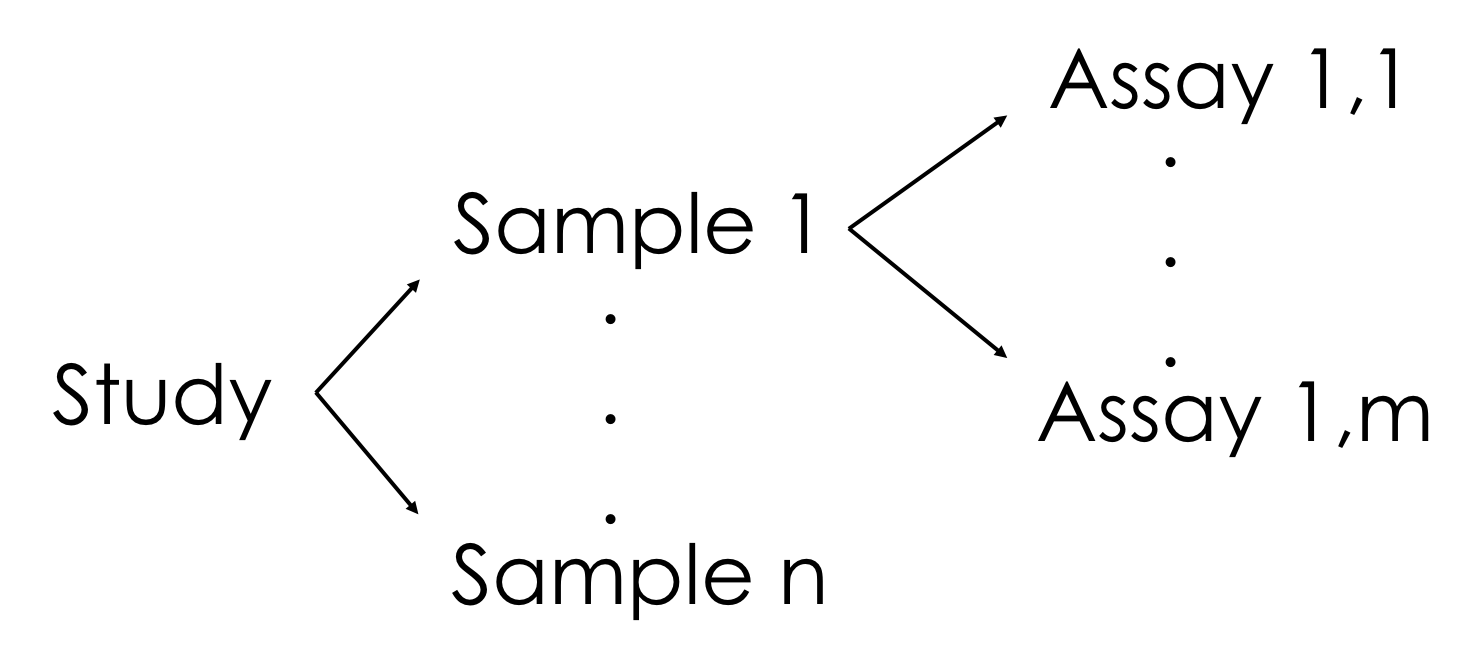
\includegraphics[scale=0.4]{figures/SRAStructure.png}}
\caption{\textbf{Structure of the SRA.} A schematic illustrating the hierarchical structure of the Sequence Read Archive.}
\label{fig:sra_structure}
\end{figure*}

\begin{figure*}[!tpb]
\centerline{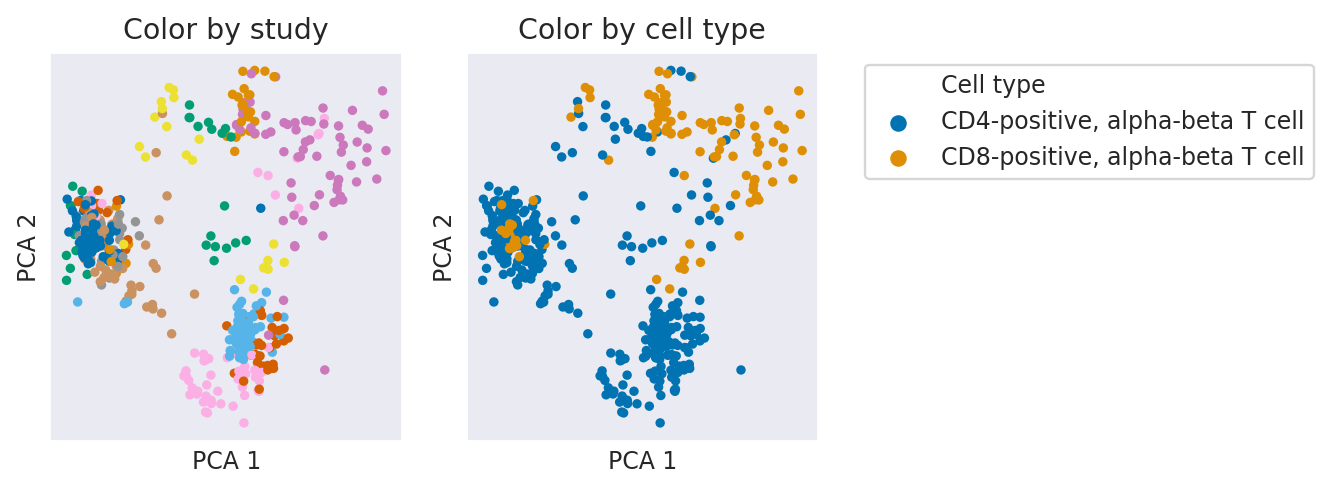
\includegraphics[width=13cm]{figures/batch_effects.png}}
\caption{\textbf{PCA plots illustrating batch effects.} PCA plots of curated CD4-positive T cell and CD8-positive T cell bulk RNA-seq samples from the SRA (described in Section~\ref{sec:primary_cell_data}). In the left-hand figure each point is colored according to the sample's study. The legend on the right pertains only to the right-hand figure.  On the right-hand figure, these same points are colored according to their cell type. Ideally, one find two tight clusters pertaining to the two presented cell types. Rather, as seen above, the clusters are largely explained by their study thus providing an example of batch effects.}
\label{fig:batch_effects}
\end{figure*}


\section{Encoding phenotypes using ontologies}

The projects presented in this work make extensive use of biomedical ontologies.  An \textit{ontology} is a structured knowledge-base that defines a set of concepts/terms within a specific domain of discourse. Besides providing the definition for each term, an ontology also encodes a directed acyclic graph (DAG) (Fig.~\ref{fig:onto_schem}) in which each term is represented by a node and each edge represents a relationship between two terms. Edges are usually labelled with a relationship-type. For example, the most common edge is the "\texttt{is\_a}" edge. Given terms $a$ and $b$, $a$ \texttt{is\_a} $b$ asserts that all instances of $a$ are also instances of $b$. Similarly, the "\texttt{part\_of}" edge represents the knowledge that one entity is a component of another entity.   

\begin{figure*}[!tpb]
\centerline{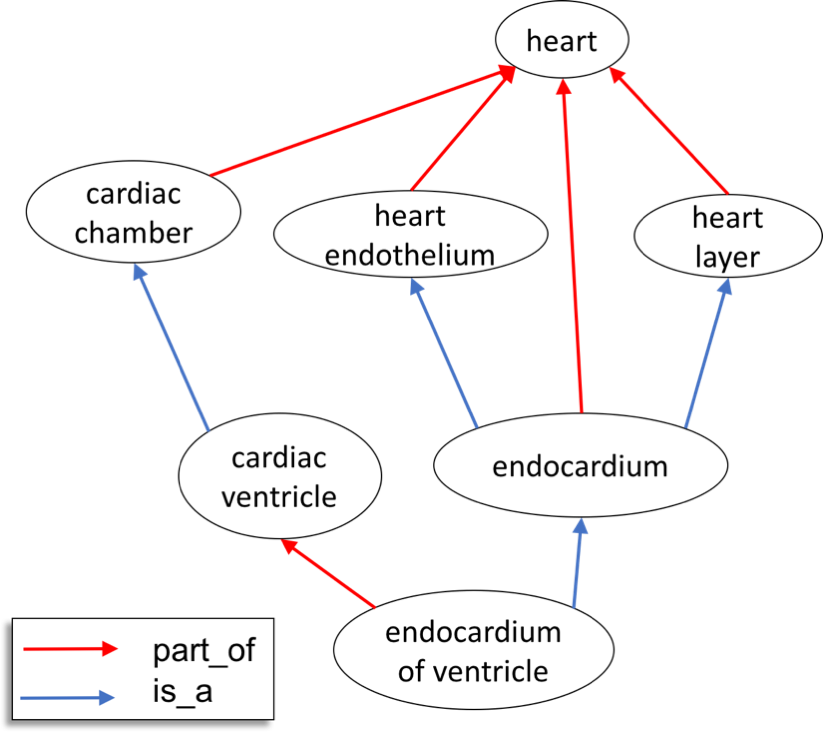
\includegraphics[scale=0.68]{figures/onto_schematic.png}}
\caption{\textbf{Example ontology graph.} A subgraph from the Uberon ontology representing anatomical entities in the heart. Red edges represent a \texttt{part\_of} relationship between terms. Blue edges represent an \texttt{is\_a} relationship between terms. }
\label{fig:onto_schem}
\end{figure*}

The fact that ontologies are hierarchically structured provides a number of advantage for the description and retrieval of public data. First, since the public data is highly diverse, the hierarchical structure enables a standardized description of data across the multiple levels of specificity of phenotypes in the database.  For example, a biological sample consisting of T cells can be labelled as ``T cell" while another sample consisting of the more specific cell type CD4-positive T cells can be labelled using a more specific term. Furthermore, the hierarchical structure also facilitates querying these diverse data. In the example above, a query for all T cells will return both samples labelled as ``T cell" and those labelled as ``CD4-positive T cell" due to ``CD4-positive T cell" being a descendant of the query in the ontology's DAG.



\section{Hierarchical multi-label classification}

Because our phenotypes are encoded as a hierarchy, the projects presented in this dissertation frame the machine learning-based TBCP task as that of \textit{hierarchical multi-label classification}.  (Fig.~\ref{fig:hierarchical_classification}).  More formally, multi-label classification is the task of learning a function 
$$f: \mathcal{X} \rightarrow \mathcal{P}(\mathcal{Y})$$ 
where $\mathcal{X}$ is the set of all possible items (in our case, $\mathcal{X} := \mathbb{R}^G$ is the set of all possible RNA-seq derived expression profiles) , $\mathcal{Y}$ is the set of all possible labels (in our case, phenotypes), and $\mathcal{P}(\mathcal{Y})$ is the powerset of $\mathcal{Y}$.  That is, given an item $x \in \mathcal{X}$, we assign $x$ a subset of labels $f(x) \subseteq\mathcal{Y}$.  Provided a DAG over the labels $Y$, hierarchical, multi-label classification imposes the restriction on $f$ that given an item $x$ and label $y \in f(x)$, the parents of $y$ in the DAG are also in $f(x)$.

Framing the TBCP task as hierarchical classification presents a number of advantages over "flat" classification in which the ontology terms are not structured hierarchically. First, the DAG of an ontology provides a rich source of prior knowledge to the classification task that remains un-utilized in flat classification.  By utilizing the hierarchy during training rather than using flat classification, more accurate classifiers can be learned (\citealp{BarutcuogluSchapireTroyanskaya2006}). Second, hierarchical classification allows for informative predictions to be made on query samples whose true phenotype label may not be included in the ontology either because the ontology is incomplete or that phenotype has yet to be discovered. Take for example the small hierarchy in Figure~\ref{fig:hierarchical_classification} encoding T cell types in the Cell Ontology (\citealp{Bard})\footnote{T cells play a pivotal role in the immune system.  They are responsible for detecting and responding to infection as well as for priming the immune system to respond to future attacks.}.  In the hypothetical scenario in which the "$\gamma\delta$ T cell"  is not in the ontology, a hierarchical classifier could label a sample of this cell type as "T cell", which would be the most apt cell type term of those available. Lastly, the use of hierarchical classification approaches allows for the placement of a bulk RNA-seq sample at a level of the hierarchy appropriate to its heterogeneity. For example, a population of cells enriched for T cells may be heterogeneous in the sub-types of T cells (e.g., $\alpha\beta$ CD4+ T cells and $\alpha\beta$ CD8+ T cells). In this case, "T cell" would be the most apt prediction.

\begin{figure*}[!tpb]
\centerline{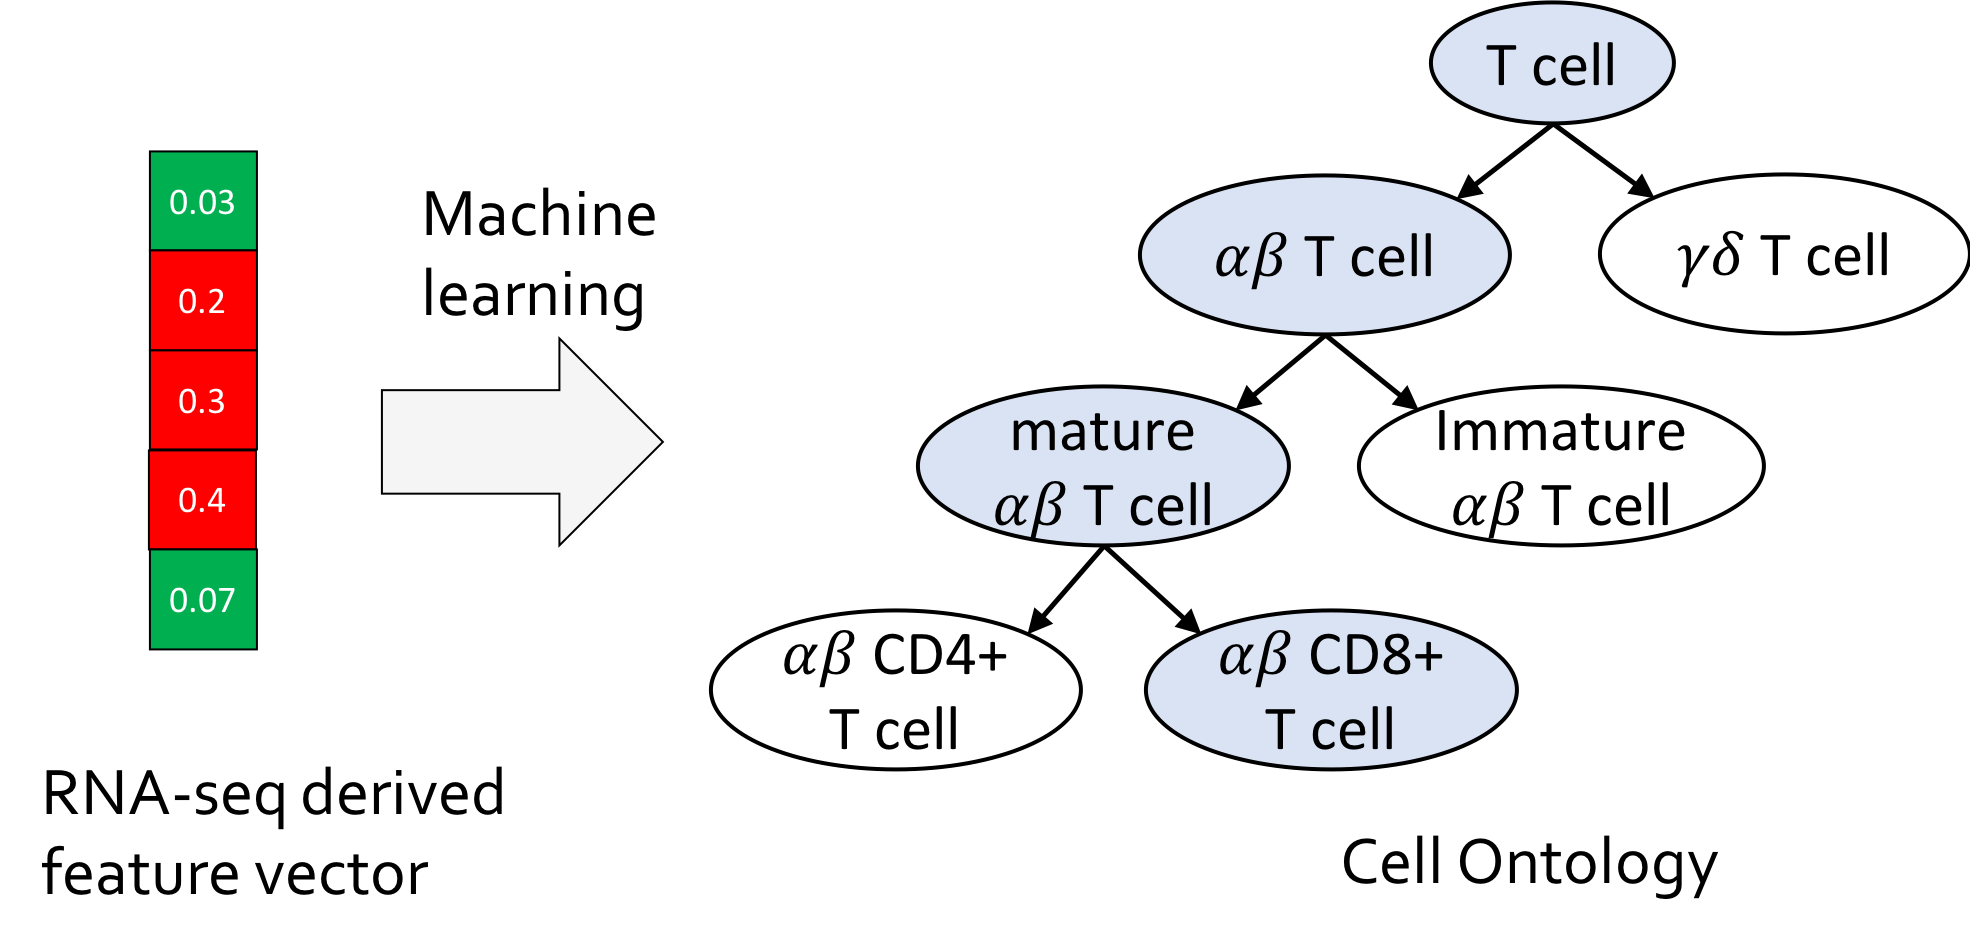
\includegraphics[width=13cm]{figures/hierarchical_classification.png}}
\caption{\textbf{Hierarchical classification.} A schematic illustrating hierarchical classification. Given an input vector of gene expression values (red indicates the gene is highly expressed and green indicates the gene is lowly expressed), the algorithm outputs a set of predicted ontology terms following the structure of the ontology (the shaded nodes on the right).}
\label{fig:hierarchical_classification}
\end{figure*}

Hierarchical classification algorithms can roughly be divided into two categories: \textit{ensemble-based} approaches and \textit{global} approaches (\citealp{Silla2011}).  Ensemble-based approaches entail training a set of independent "flat" classifiers, where each classifier corresponds to a node of the hierarchy, and then aggregating the outputs of these classifiers so that they are consistent with the hierarchy\footnote{Because each classifier makes a prediction independently from the rest, these predictions may be logically inconsistent with the hierarchy. This will occur if a classifier outputs a positive prediction for a given node, but it's parent classifier outputs a negative prediction.}.  Ensemble-based approaches can be further divided according to how each flat classifier is trained. Some methods train independent one-vs.-rest classifiers for each node, where each classifier makes a binary decision as to whether the query instance belongs to the given node or not. Examples of these approaches include Baysian Network Correction (\citealp{BarutcuogluSchapireTroyanskaya2006}) and projection-based approaches (\citealp{Obozinski2008}).  Other ensemble-based approaches take a different strategy in which classification is performed in a top-down fashion and each node's classifier makes a binary decision as to whether the query item belongs to the given node conditioned on the fact that it belongs to the parents of that node (\citealp{Obozinski2008, CesaBianchi2006}). In contrast, in the global approach, classification is inextricably intertwined with the hierarchy of the labels. Examples of global approaches include decision tree-based approaches (\citealp{Vens2008}), supervised hierarchical latent Dirichlet allocation (\citealp{Perotte2011}), and kernel dependency estimation approaches (\citealp{Bi2011}).  
  
In this work, we explore ensemble-based approaches because they admit more flexibility in their development. This is because, in contrast with global approaches, ensemble-based approaches decouple the hierarchical classification process into two steps: first, each independent classifier makes its predictions and then these predictions are aggregated to ensure that they are consistent with the hierarchy.  Thus, the design decisions regarding the independent classifiers are independent from the design decisions regarding how the predictions are made to be consistent with the hierarchy. 

\section{This dissertation}

In this section, we outline the contributions presented in this thesis.  These contributions span multiple stages of the machine learning pipeline, from acquiring labelled training data (Chapter~\ref{chap:1}), to developing machine learning algorithms (Chapters \ref{chap:2} and \ref{chap:3}) (Fig.~\ref{fig:phenotyping_dataflow}).  We preview the contributions of this thesis in the subsections below:
 
\subsection{Normalized sample-specific metadata for the SRA}

In the first project, we address the challenge of obtaining ground-truth, labeled training data from the SRA for performing supervised training of a phenotype classifier. Such ground truth labelings are difficult to obtain due to the poor structure of the sample-specific metadata in the SRA.  In this project we developed a novel computational approach for normalizing this metadata by tagging sample entries in the SRA with terms from biomedical ontologies. Existing approaches treat metadata normalization as a \textit{named entity recognition} (NER) problem, where the goal is to tag metadata with terms from controlled vocabularies when that term is mentioned explicitly in the metadata text. We reframed this problem as an inference task, in which we seek to tag the metadata with only those terms that describe the underlying biology of the described sample rather than tag the metadata with all mentioned terms. We found that this approach yielded mapped ontology terms with fewer false positives than existing approaches that frame the problem as NER. 

\subsection{Hierarchical cell type classification using mass, heterogeneous RNA-seq data from human primary cells}

In the second project, we use the mapped ontology terms produced by the first project in order to supervise the training of RNA-seq-based phenotype classifiers. We specifically focus on the cell type prediction task: given an RNA-seq sample, we wish to predict the cell type from which the sample was derived.  Cell type prediction is an important step in many transcriptomic analyses, including that of annotating cell types in single-cell RNA-seq datasets. This work represents the first concerted effort towards the cell type  prediction task that utilizes the full potential of publicly available RNA-seq data.  Further, we explore the novel application of hierarchical machine learning classifiers to leverage prior knowledge of cell type hierarchies, specifically, the Cell Ontology. To this end, we pushed the state-of-the-art in cell type prediction accuracy of bulk and single-cell RNA-seq.  

\subsection{Cell type classification of sparse single-cell RNA-seq data}

In the third project, we build on the second project in order to address the task of cell type prediction on \textit{sparse} scRNA-seq data from novel droplet-based technologies.  These droplet-based scRNA-seq technologies are enabling the sequencing of higher numbers of cells at the cost of a lower read-depth per cell, which results in expression measurements for fewer genes per cell.  In this project, we explore the effects of applying cell type classifiers trained on dense, bulk RNA-seq data to sparse scRNA-seq data and propose a novel probabilistic generative model for adapting the bulk-trained classifiers to sparse input.

\begin{figure*}[!tpb]
\centerline{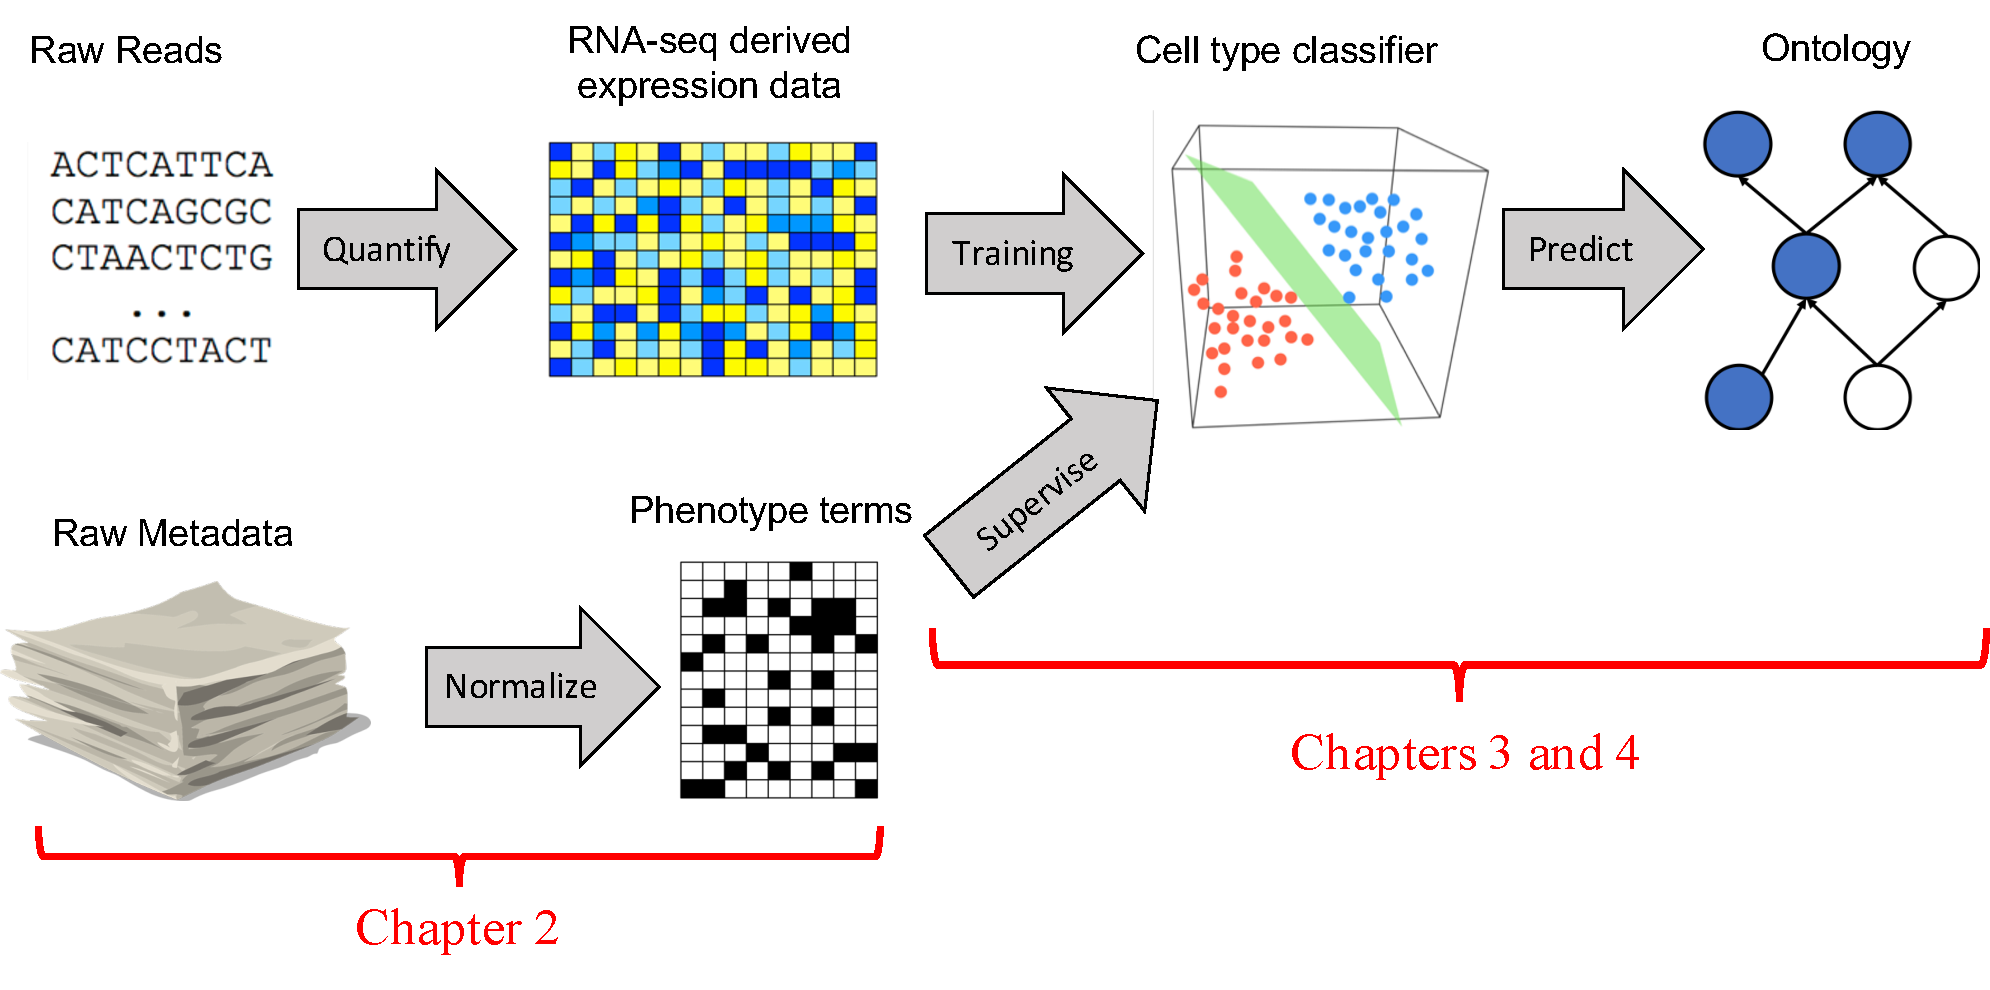
\includegraphics[width=13cm]{figures/phenotyping_dataflow.pdf}}
\caption{\textbf{TBCP Overview.} A schematic illustrating the components of the transcriptome-based cellular phenotyping task.}
\label{fig:phenotyping_dataflow}
\end{figure*}




%However, these opportunities are impeded by a number of challenges including poorly structured metadata and data heterogeneity.  In this thesis, I present three related projects that address these challenges via the development of novel computational methodologies. 



















\chapter{Normalization of metadata in the Sequence Read Archive} \label{chap:1}

The work in this chapter was previously published as \textit{MetaSRA: normalized human sample-specific metadata for the Sequence Read Archive} (\citealp{Bernstein2017}). 

\section{Background}

The SRA promises great biological insight if one could analyze the data in the aggregate; however, the data remain largely underutilized, in part, due to the poor structure of the metadata associated with each sample. The rules governing submissions to the SRA do not dictate a standardized set of terms that should be used to describe the biological samples from which the sequencing data are derived. As a result, the metadata include many synonyms, spelling variants and references to outside sources of information. Furthermore, manual annotation of the data remains intractable due to the large number of samples in the archive. For these reasons, it has been difficult to perform large-scale analyses that study the relationships between biomolecular processes and phenotype across diverse diseases, tissues and cell types present in the SRA.

Our goal in this work is to provide structured descriptions of the human biological samples used in the SRA in order to enable aggregate analysis, as well as reanalysis, of these data.  This task is challenging because it requires discriminating between information that describes the biological sample from information that describes other entities such as the sample's study, sequencing protocol, and lab. A solution to structuring the sample-specific information must address the metadata's semantics. 

Existing methods for normalizing biomedical text focus on annotating the text with terms in a controlled vocabulary, usually in the form of a biomedical ontology.  One can approach the task of annotating metadata using either a manual or automated approach.  Manual annotation allows for high accuracy at the cost of low throughput.  For example, the RNASeqMetaDB  provides a database of manually annotated terms associated with a set of mouse RNA-seq experiments (\citealp{Guo}).  This database describes only 306 RNA-seq experiments, which represents a small subset of all experiments in the SRA. 

In contrast, automated annotation allows higher throughput at the cost of lower accuracy. Methods for automating the normalization of biomedical metadata frame the task as that of \textit{entity recognition}. Entity recognition is the process of automatically recognizing and linking entities in natural language text to their corresponding entries in a controlled vocabulary.  Tools that take this approach include ConceptMapper (\citealp{Tanenblatt}), SORTA (\citealp{Pang}), ZOOMA (\citealp{Misha}), and the BioPortal Annotator (\citealp{Noy}).  Furthermore, there have been efforts to utilize such tools to automatically normalize large biomedical metadata sets.  For example, work by \cite{Shah} automatically annotated samples and studies in the Gene Expression Omnibus (GEO) (\citealp{Barrett2013}) and other sources of biomedical metadata. Similarly, work by \cite{Galeota} annotated samples in GEO using ConceptMapper. 

We assert that entity recognition alone is insufficient for automating the normalization of the SRA's sample-specific metadata.  Rather, since many of the sample's descriptions mention ontology terms that describe extraneous entities (such as the study and experiment), a suitable solution should seek to extract \textit{only} those terms that are being used to describe the biology of the sample. Biomedical entity recognition tools are best suited for data submitters who wish to facilitate annotation of their metadata before submission. Such tools do not adequately filter terms that do not describe the biology of the sample because they do not attempt to understand the fine-grained semantics of the text.

We further assert that important biological properties are often numerical and are not captured by ontology terms alone.  Such terms include age, time point, and passage number for cell cultures. To the best of our knowledge, the problem of extracting real-value properties from metadata has yet to be addressed.

Lastly, we assert that ontology terms alone do not always provide enough context to understand the type of sample being described.  For example, a cell culture that consists of stem cells differentiated into fibroblast cells may be annotated as both ``stem cells'' and as ``fibroblast.''  Such annotation leaves ambiguity as to whether the sample was differentiated from stem cells, or rather, was reprogrammed into a pluripotent state from primary fibroblasts.  We assert that each sample should be categorized into a specific sample-type that captures the process that was used to obtain the sample.  

To address problems in the SRA's metadata, we developed MetaSRA: a normalized encoding of biological samples in the SRA, along with the novel computational pipeline with which it was automatically constructed.   MetaSRA encodes the metadata for each sample with a schema inspired by that used in the ENCODE project (\citealp{Malladi}).  This schema is comprised of three parts:
\begin{enumerate}
\item Sample labels, using terms from the following biomedical ontologies: Disease Ontology (\citealp{Kibbe}), Cell Ontology (\citealp{Bard}), Uberon (\citealp{Mungall}), Experimental Factor Ontology (EFO) (\citealp{Malone}), and the Cellosaurus (\citealp{Bairoch2018}). 
\item A sample-type classification, with six sample-type categories similar to those used by ENCODE.
\item Standardized numerical properties of the sample.
\end{enumerate}
The first two parts are shared with the ENCODE schema, with the last part being a MetaSRA-specific extension. Currently, MetaSRA encodes all human samples utilized in RNA-seq experiments on the Illumina platform; however, future work will expand MetaSRA to other species and assays.

\begin{figure*}[!tpb]
\centerline{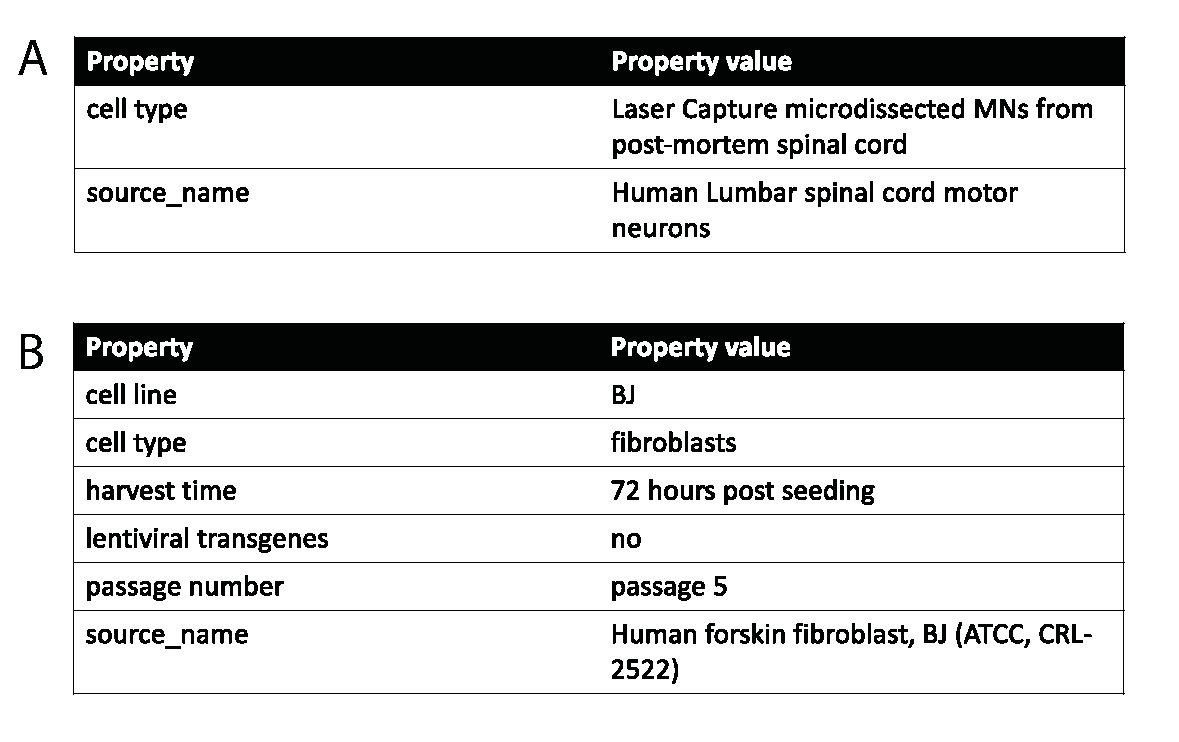
\includegraphics[width=13cm]{figures/example_key_vals.eps}}
\caption{\textbf{Example metadata entries.} (A) Sample-specific key-value pairs describing sample SRS1217219. Note that the values encode natural language text. (B) Sample-specific key-value pairs describing sample SRS872370. Note the reference to an external cell lin
e BJ. We also note that `forskin fibroblast' is an incorrect spelling. Lastly, the value `no' negates the key `lentiviral transgenes.'}
\label{fig:example_raw_key_vals}
\end{figure*}

\section{Task definition}

\subsection{Mapping samples to ontologies}

Like the ENCODE project, we label each biological sample using biomedical ontologies. We define the task of mapping samples to ontologies as follows: given a set of samples $\mathcal{S}$, a set of ontology terms $\mathcal{O}$, and set of relationship-types $\mathcal{R}$, we seek a function $f: \mathcal{S} \rightarrow \mathscr{P}(\mathcal{O})$, where $\mathscr{P}(\mathcal{O})$ is the powerset of $\mathcal{O}$, such that given a sample $s$, for each $o \in f(s)$, there exists a relationship-type $r \in \mathcal{R}$ that relates the sample $s$ to the ontology term $o$.   We restrict $\mathcal{R}$ to the following types of relationships:
\begin{itemize}
    \item \textbf{has phenotype}:  Maps samples to phenotypic or disease terms. 
    \item \textbf{derives from}:   Maps samples to cell lines or, when the sample consists of differentiated cells, to stem cell terms. 
    \item \textbf{part of}:    Maps samples to the anatomical entity from which it was extracted. 
    \item \textbf{consists of cells of type}:  Maps samples to their constituent cell types. 
    \item \textbf{underwent}: Maps samples to ontology terms that describe a medical or experimental protocol. \vspace*{1pt}
\end{itemize}
We restrict our use of ontology terms to only ``biologically significant'' terms.  An ontology term $o$ is deemed biologically significant if given two samples $s_1, s_2 \in \mathcal{S}$  where $f(s_1) \subset f(s_2)$ and $f(s_2) \setminus f(s_1) = \{o\}$
 there likely exists a difference in gene expression or other measurable difference in biochemistry between the two samples.  In simpler terms, an ontology term $o$ is deemed biologically significant if given two samples with equivalent descriptions barring that one sample can be described by $o$ and the other cannot, a significant difference in the biochemistry of the cell may exist between the two samples. For example, the ontology term for ``cancer'' is biologically significant, whereas the term ``organism'' is not because all samples are trivially derived from an organism.   We manually searched the ontologies for biologically significant terms that are near the roots of the ontologies' directed acyclic graphs.  We then assume that all children of a biologically significant term are also biologically significant and retrieve all children of the manually selected nodes. We map samples to only biologically significant terms in the ontologies.  An example of a standardized sample is shown in Figure~\ref{fig:project_flow}.
 
 \subsubsection{Discriminating between term mentions and term mappings}

Our goal in mapping samples to ontology terms goes beyond named entity recognition.  Rather than finding all occurrences or ``mentions'' of ontology terms in the metadata, we attempt to infer which labels adequately describe the biological sample being described.  A term may be mentioned, but not mapped as well as mapped, but not mentioned. 

For example, consider a sample's description that includes the following text: \texttt{Metastatic castration resistant}\\ \texttt{prostate cancer}.  If we consider the Uberon and Disease Ontology, we see that the string ``prostate cancer'' mentions three terms in these ontologies: ``prostate gland'', ``cancer'', and ``prostate cancer.'' Of these terms, only ``cancer'' and ``prostate cancer'' are mapped because they are related to the sample through the ``has phenotype'' relationship. The string ``prostate'' is not not mapped because it localizes the disease rather than the sample.  There is no relationship-type in $\mathcal{R}$ that associates the sample with ``prostate.''  By prohibiting the mapping to ``prostate'', we remove ambiguity as to whether the sample was derived from an organism with a prostate-related disease, or from prostate tissue itself.  More generally, whenever a sample maps to an anatomical entity, we are asserting that the sample originated from that site.

To provide an example in which an ontology term should be mapped, but is not mentioned, consider a sample described with the key-value pair \texttt{passage: 4}.  The Cell Ontology term for ``cultured cell'' is not mentioned in this description; however, by the fact that it was explicitly stated that the cell was passaged, we can infer that the sample consists of cultured cells. Thus we map the sample to ``cultured cell'' via the ``consists of cells of type'' relationship.

\subsubsection{Discriminating between explicit and consequent mappings}

We distinguish between two types of mappings: those that are explicit in the metadata and those that can be inferred from the explicit mappings.   We refer to the latter as ``consequent mappings.''  For example, the ontology term for ``female'' is explicitly mapped from the key-value pair, \texttt{sex: female}, because the author is explicitly communicating the fact that this sample maps to ``female'' through the ``has phenotype'' relationship.

A sample ``consequently'' maps to an ontology term if, using external knowledge, one can logically conclude that the sample maps to the term. The premier example of such a case arises when a sample maps to a cell line.  In such a case, the sample would consequently map to terms that describe this cell line. For example, given the key-value pair \texttt{cell line: MCF-7}, the sample would consequently map to ``adenocarcinoma'' because the MCF-7 cell line was established from a breast adenocarcinoma tumor.  MetaSRA includes both explicit and consequent mappings.

\subsection{Extracting real-value properties}
In addition to mapping samples to ontology terms, we also annotate samples with real-value properties that are described in the metadata.  We structure each real-value property as a triple ($property$, $value$, $unit$) where $property$ is a property ontology term in the EFO, $value \in \mathbb{R}$, and $unit$ is an ontology term in the Unit Ontology (\citealp{Gkoutos}).  For example, the raw key-value pair \text{\texttt{age: 20 years old}} would map to the tuple (``age'', 20, ``year'').

\subsection{Predicting sample-type category}

Like the ENCODE project, we categorize samples into their respective sample-type using categories similar to those used by ENCODE.  These categories consist of \texttt{cell line}, \texttt{tissue}, \texttt{primary cell}, \texttt{stem cell}, \texttt{in vitro differentiated cells}, and \texttt{induced pluripotent stem cell line}. Whereas ENCODE uses an \texttt{immortalized cell line} category, we instead use the category \texttt{cell line} to generalize to any cells that have been passaged multiple times, which include those from finite cell lines.  Figure~\ref{fig:sample_type_def} illustrates how we define each sample-type category based on the methods by which the sample was obtained. We note that we call an isolated cell sample a ``stem cell" if the targeted cell type has the ability to differentiate.  Thus, the ``stem cell" category includes any cell type that is pluripotent, multipotent, or oligopotent.   

\begin{figure}[htbp]
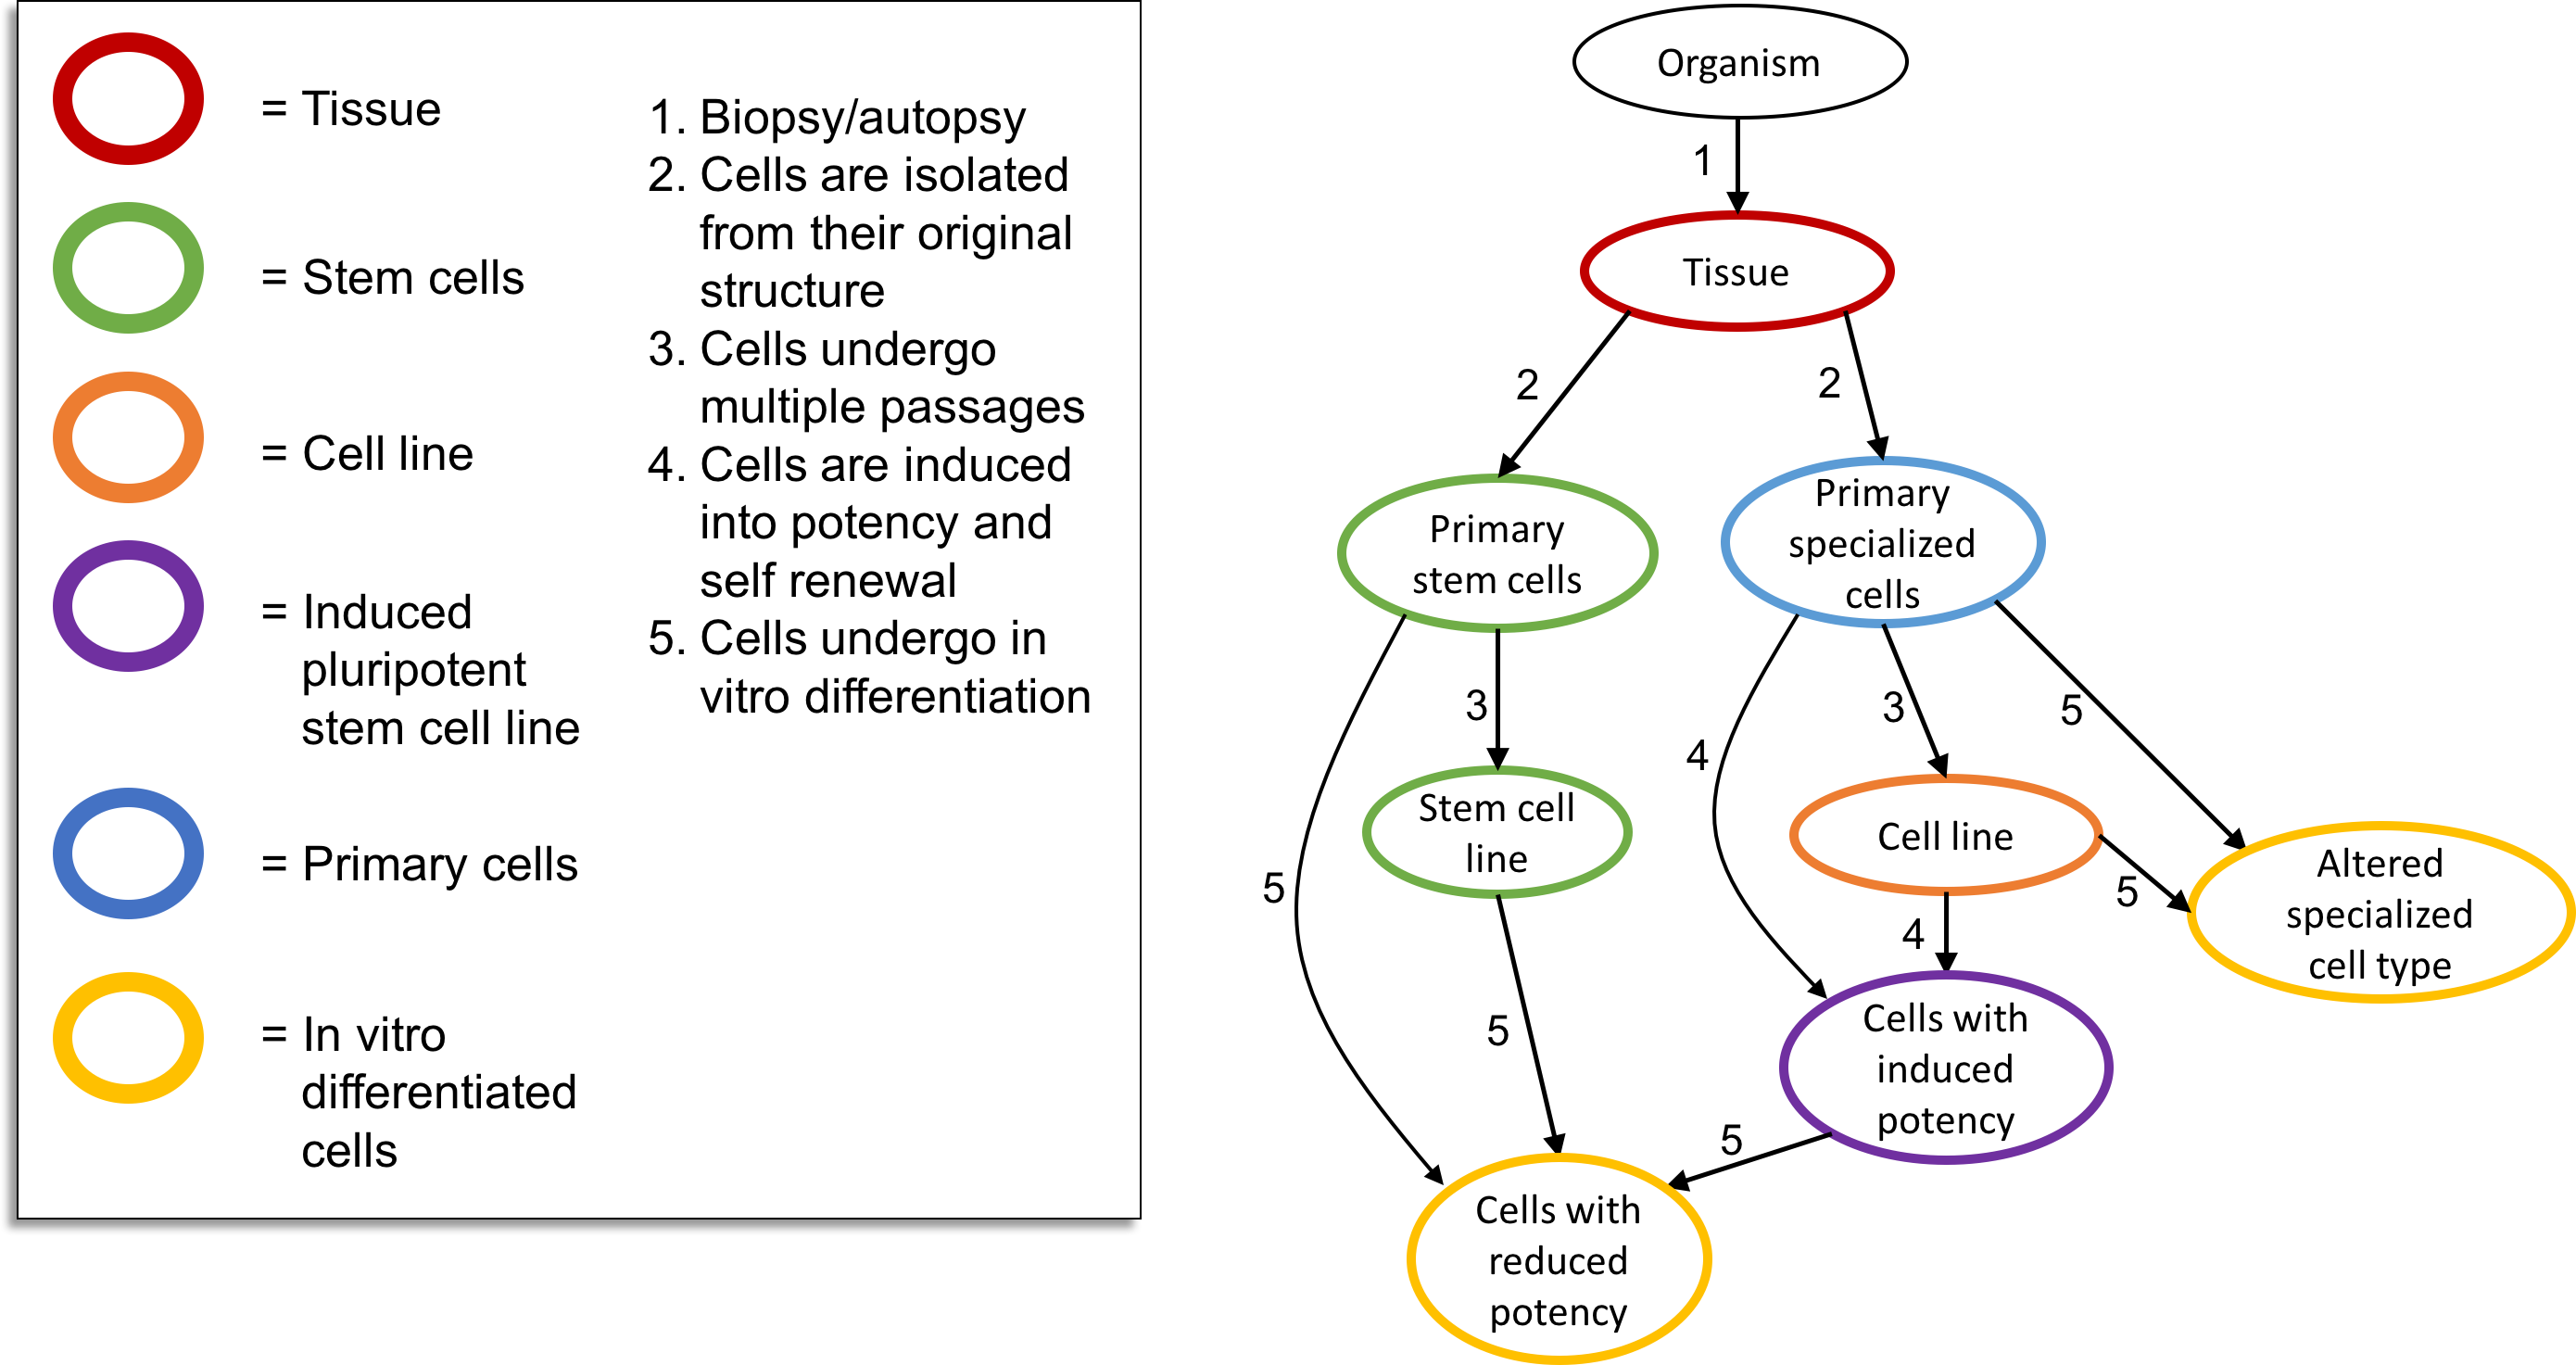
\includegraphics[width=13cm]{figures/sample_type_definition.png}  
\caption{\textbf{Sample-type definitions.} A graph illustrating how sample-type categories are defined. Each node in the graph represents a biological sample.  Arrows between nodes represent procedures carried out on the sample.  Nodes are colored according to their sample-type category.}
\label{fig:sample_type_def}
\end{figure}





\section{Data}

\begin{figure*}[!tpb]
\centerline{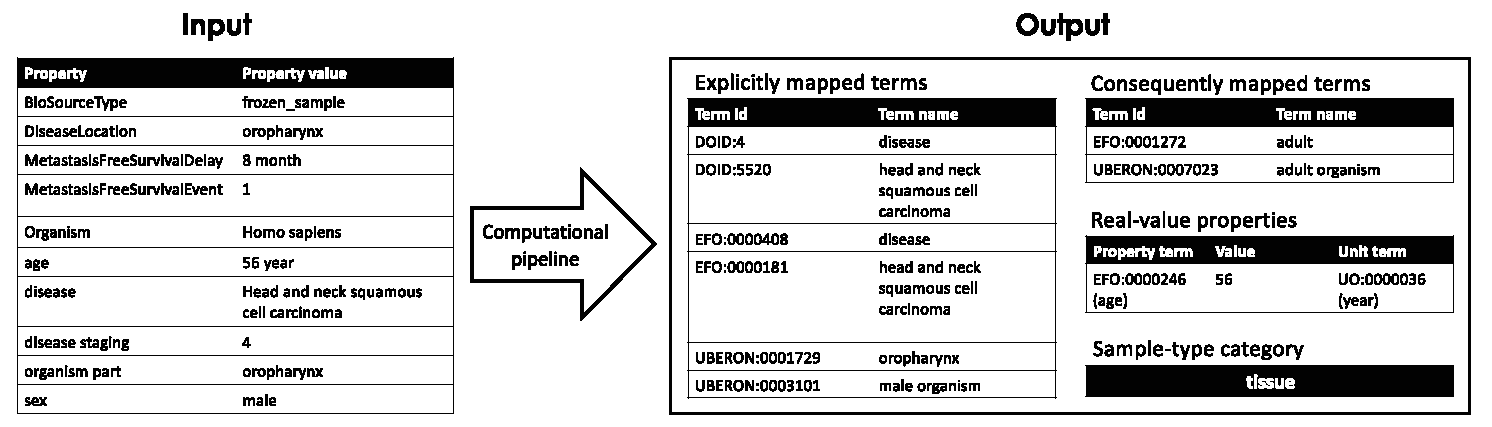
\includegraphics[width=13cm]{figures/project_flow.pdf}}
\caption{\textbf{Example of metadata normalization.} An example of the metadata normalization process for sample ERS183215. We extract explicit mappings, consequent mappings, real-value properties, and the sample-type category for each set of sample-specific key-value pairs in the SRA.}
\label{fig:project_flow}
\end{figure*}

We standardized all human samples assayed by RNA-seq experiments on the Illumina platform.  Metadata was retrieved from the SRAdb (\citealp{Yuelin}) downloaded on 09/05/2016.  The BioSample's sample-specific key-value pairs are  stored in the ``attribute'' field of the ``sample'' table in the SRAdb.  Our data set consists of 75,038 samples, of which, 73,407 are associated with a non-empty set of descriptive key-value pairs.

The samples processed belong to 2,681 distinct studies and the number of samples contained in each study varies by several orders of magnitude (Fig.~\ref{fig:dataset}C).  These studies can be partitioned into 88 ``large" ($\geq 100$ samples) and 2,593 ``small'' ($< 100$ samples) studies, with the ``large'' studies constituting 57\% of all samples processed.  Due to the fact that samples belonging to a common study are described similarly, we argue that it is tractable to annotate samples belonging to the modest number of ``large'' studies using hand-tuned study-specific methods.  In contrast, the large number of ``small'' studies and the diversity of their associated descriptions makes the process of designing study-specific methods for all of these studies intractable.  We therefore focused our evaluations on samples belonging to ``small'' studies, with future work involving hand-tuning the normalization of samples from ``large'' studies.

\begin{figure*}[!tpb]
\centerline{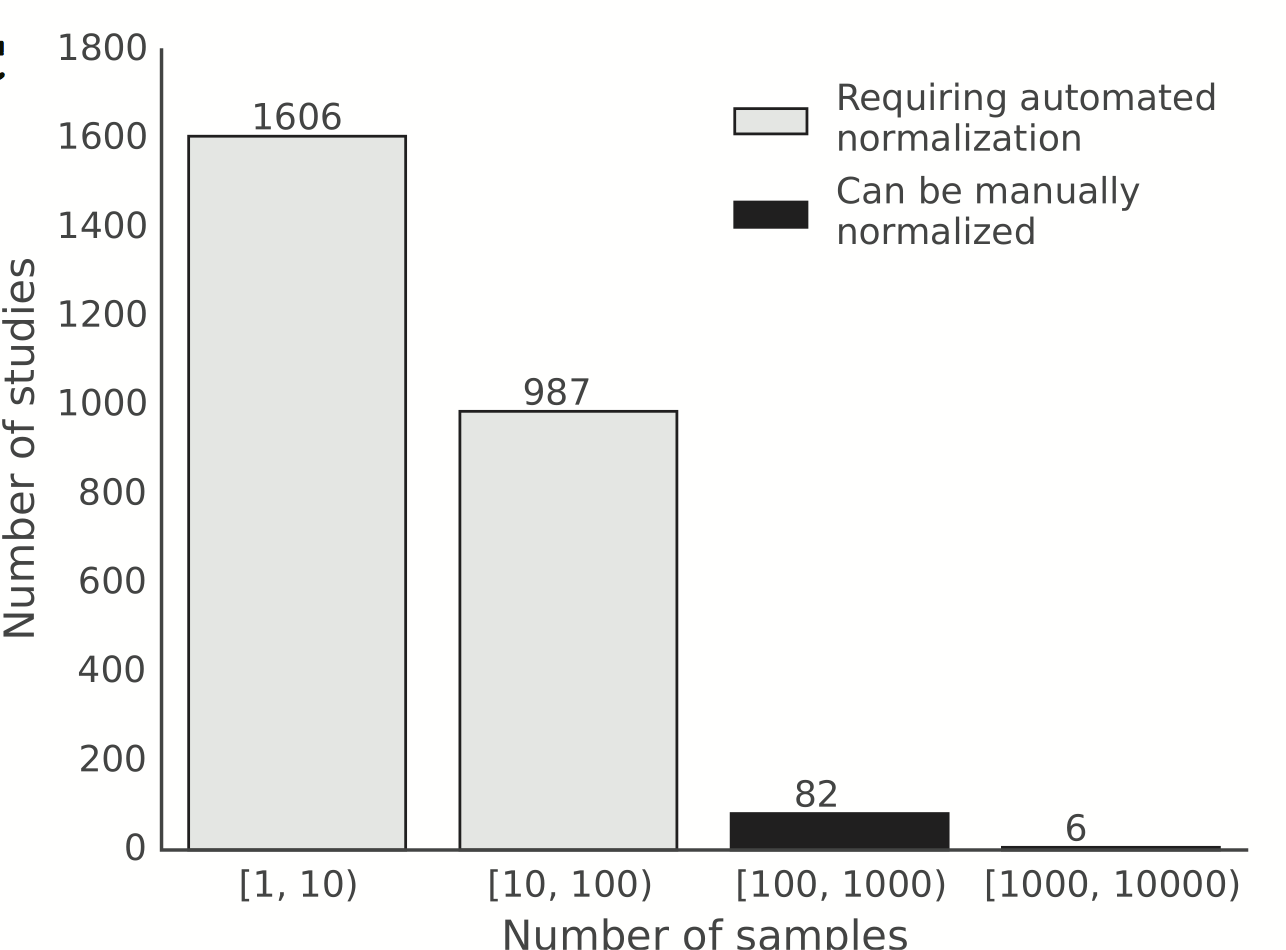
\includegraphics[scale=0.20]{figures/data_set_figure.png}}
\caption{\textbf{Dataset overview} Histogram of the number of samples per study for human RNA-seq experiments using the Illumina platform. We assert that the 88 studies each with at least 100 samples can be semi-manually normalized using study-specific methods.}
\label{fig:dataset}
\end{figure*}





\section{Methods}

Framing the ontology term mapping task as a multi-class classification problem in which each ontology term is a class, a machine learning approach might seem to be a natural choice.  However, such an approach would require a training set that includes multiple examples of samples that map to each ontology term.  Due to the large number of ontology terms, obtaining such a training set is unfeasible.  Thus, for the ontology term mapping and real-value property extraction tasks, we took an algorithmic approach.  In contrast, the sample-type classification task involves only a handful of possible classes and we can easily create, via manual annotation, a training set containing multiple samples from each class.  Thus, for this latter task, we used a statistical machine learning approach.

\subsection{Mapping samples to ontologies}

At the core of our method is a graph data structure for maintaining the provenance of each derived ontology term.  This graph, which we call a Text Reasoning Graph (TRG), provides a framework for maintaining the provenance of extracted ontology terms, and for writing rules and operations that can reason about which terms should be mapped versus which are merely mentioned.  Nodes in the TRG represent artifacts derived from the original metadata text. Such artifacts may be $n$-grams, inflectional variants, or synonyms.  Other nodes in the graph represent mapping targets such as ontology terms or real-value property tuples.  Edges between artifacts represent derivations from one artifact to another. An edge between an artifact and an ontology term represents a lexical match between the artifact and the ontology term.  

We implemented a computational pipeline that is composed of a series of stages that constructs the TRG.  To start, the pipeline accepts the raw key-value pairs and constructs an initial TRG. Then, each stage operates on the TRG by modifying its nodes and edges. Figure~\ref{fig:example_trg} depicts the subgraph of a final TRG that maps a key-value pair to a set of ontology terms.   By maintaining the provenance of each derived ontology term we can implement custom reasoning operations that more accurately determine which terms describe the sample.  Such reasoning operations utilize the graph structure to filter out ontology terms for which there is no relationship-type in $\mathcal{R}$ that describes the relationship between the sample and the ontology term.  

\begin{figure*}
\centerline{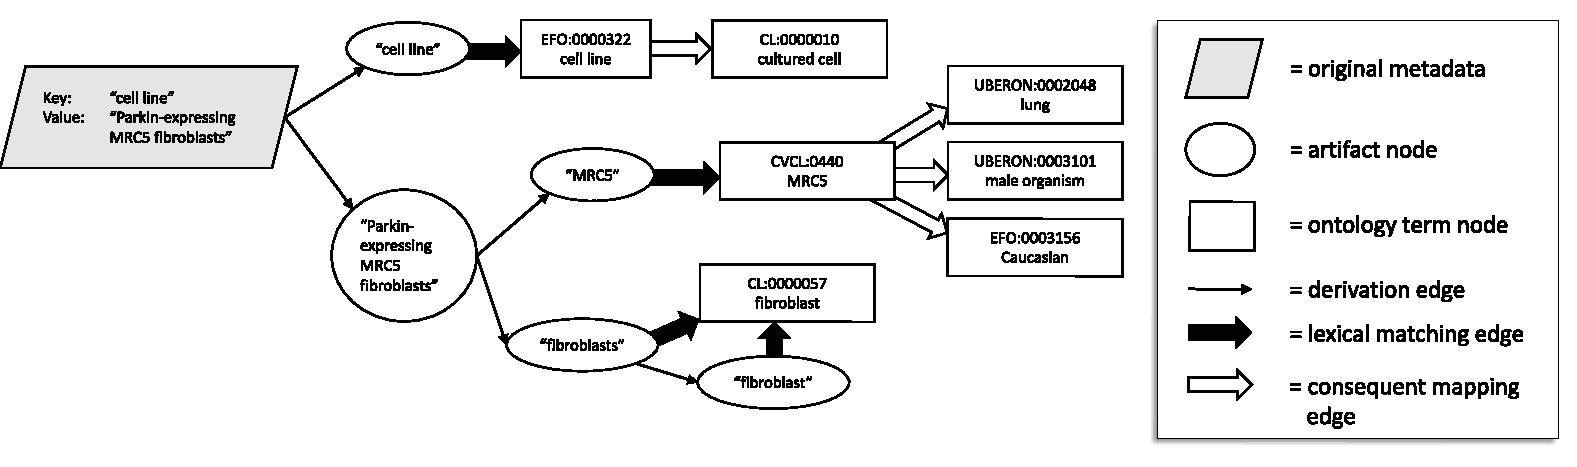
\includegraphics[width=13cm]{figures/example_TRG.pdf}}
\caption{\textbf{Example Text Reasoning Graph.} A subgraph of the TRG constructed from sample SRS1212219 illustrating the graph data structure that our pipeline maintains as it reasons about the sample.  This framework allows us to maintain the context of each artifact. For example, we map to the MRC5 cell line only because there is a mapping to the ``cell line'' ontology term in the graph emanating from the key.  We also note the terms for ``lung'', ``male organism'', and ``Caucasian'' were mapped to the MRC5 cell line from the ATCC cell bank data and are thus \textit{consequent mappings}.}
\label{fig:example_trg}
\end{figure*}

In the following sections we describe the most notable stages of the pipeline. Full details are provided in Section~\ref{sec:mapping_pipeline}.

\subsubsection{Filtering key-value pairs}

Before initializing the TRG, we filter key-value pairs from the metadata where either the key or value appears in a set of blacklisted keys and values.  This blacklist of keys contains those that describe a property that does not pertain to the biology of the sample, such as ``study name'' and ``biomaterial provider.''  The blacklist of values include those that negate the key, such as ``none'' or ``no.''  For example, the key-value pair \texttt{is tumor: no} is removed because the value \texttt{no} negates the property \texttt{is tumor}. 

\subsubsection{Artifact generation}

We define an artifact to be any string that is derived from a substring of the original metadata text.  Such artifacts include include $n$-grams, lower-cased words, and inflectional and spelling variants of words in the metadata.  An artifact node in the TRG represents a single artifact.  Several stages of the pipeline generate new artifact nodes from existing artifact nodes and draw edges from original to derived artifacts.   One such stage derives inflectional and spelling variants from existing artifacts using the National Library of Medicine's SPECIALIST lexicon (\citealp{Browne}).  For example, given an artifact node representing the pluralized noun ``fibroblasts'', this stage will create a node for the singular noun ``fibroblast'' and draw a directed edge from ``fibroblasts'' to ``fibroblast'' (Fig.~\ref{fig:example_trg}).

\subsubsection{Matching artifacts to ontologies}

We perform fuzzy string matching between all artifacts and  ontology terms to find all exact matches and minor misspellings (for misspelling criteria, see supplementary materials). For example, in Figure~\ref{fig:example_trg}, both the strings ``fibroblasts" and ``fibroblast" fuzzily match to the ontology term for ``fibroblast".

In general, fuzzy matching is computationally expensive.  To speed up this process, we pre-compute a  metric tree index (\citealp{Bartolini}) for all ontology term names and synonyms. The index allows us to filter for ontology term strings that are nearby the query string in edit space.  We then explicitly compute the edit distances to these nearby strings. 

\subsubsection{Graph reasoning}

Certain stages of the pipeline utilize the structure of the TRG.  We refer to such steps as ``reasoning'' steps.  For example, we remove extraneous mappings to cell line terms by searching the graph emanating from the key for a lexical match to ontology terms such as ``cell line'' and ``cell type.''  If such a match is \textit{not} found, we search the graph emanating from the value for artifacts that have a lexical match to a cell line ontology term and remove all such ontology term nodes.  This process is important for removing false positives due to the fact that names of cell lines are often similar to gene names and acronyms. For example, ``Myelodysplastic Syndromes'' is often shortened to ``MDS.'' MDS also happens to be a cell line in the Cellosaurus. Other examples of stages that utilize the graph structure are described in the supplementary materials.

\subsubsection{Inferring consequent terms}

Certain stages of the pipeline attempt to map the sample to terms that are not explicitly mentioned in the raw metadata text describing the sample.  We refer to such mapped terms as \textit{consequent terms}.  We map to consequent terms by consulting external knowledge bases.  The pipeline uses two external knowledge bases: a cell line database and a rules database.

First, we created a database of mappings between cell lines and ontology terms.  We obtained this data by scraping from the ATCC website (\href{https://www.atcc.org}{https://www.atcc.org}). We scraped cell line metadata for all cell lines that are present in the Cellosaurus.  To construct mappings between cell lines and ontology terms, we ran a variant of our pipeline on the scraped cell line data. Our pipeline uses this database as follows: our pipeline will draw edges between mapped cell line ontology term nodes and the ontology terms that describe the biology of the cell line.   For example, in Figure~\ref{fig:example_trg}, the ontology term for the MRC5 cell line has an edge to ``lung", ``male", and ``Caucasian" because this cell line was derived from lung tissue of a Caucasian male aborted fetus (\citealp{Jacobs}).

Second, we created a small rules database that dictates how certain ontology terms logically imply other ontology terms.  For example, in Figure~\ref{fig:example_trg} the term ``cell line" has an edge to the term ``cultured cell" because all cell lines are grown in a culture.  

\subsubsection{Maximal phrase-length mapping}

It is a common occurrence for disease ontology terms to include anatomical entities in their name. For example, ``breast cancer'' includes ``breast'' as a substring. As previously discussed, under our framework, it would be incorrect to map ``breast'' to a sample solely based on a mention of ``breast cancer'' in its metadata because ``breast'' localizes the cancer, but does not localize the origin of the sample.  Whereas it is entirely possible that such a sample was indeed derived from breast tissue, without additional information we cannot eliminate the possibility that the sample originated from some other tissue, such as from a malignant site.  In this example, we maintain a conservative approach and avoid mapping to ``breast.''  We implement this process by having each artifact node keep track of the original character indices in the metadata from which it was derived. After mapping all artifacts to the ontologies, we remove all ontology terms that were lexically matched with an artifact node that is subsumed by another artifact node that matches with an ontology term.  

\subsubsection{Linking ontologies}

The domain covered by the EFO overlaps with many of the other ontologies because it includes cell types, anatomical entities, diseases, and cell lines.  In many cases, the EFO is inconsistent with other ontologies in how it draws edges between terms.  For example, the term ``lung adenocarcinoma'' and ``adenocarcinoma'' are present in both the Disease Ontology and the EFO; however ``adenocarcinoma'' is a parent of ``lung adenocarcinoma'' in the Disease Ontology but not in the EFO.  These inconsistencies pose a problem when we apply our maximal phrase-length mapping process.   For example, when a sample maps to ``lung adenocarcinoma'' and ``adenocarcinoma'', we remove ``adenocarcinoma'' because it is a substring of ``lung adenocarcinoma.''  This is valid for the Disease Ontology because the term for ``adenocarcinoma'' is implied by ``lung adenocarcinoma'' by its position in the ontology.  However, this results in a false negative for the EFO version of this term.  

To counteract this problem, we link EFO terms to terms in the other ontologies.  Two terms are linked when they share the same term-name or exact-synonym.  Then, when an artifact maps to a term, we traverse the term's ancestors and map to any terms that are linked to those ancestors.   In the case of ``lung adenocarcinoma'', we would traverse the ancestors of this term in the Disease Ontology and map to the EFO's ``adenocarcinoma'' because it is linked to the Disease Ontology version of this term. Figure~\ref{fig:linked} illustrates this process. 

\begin{figure}[htbp]
\centering
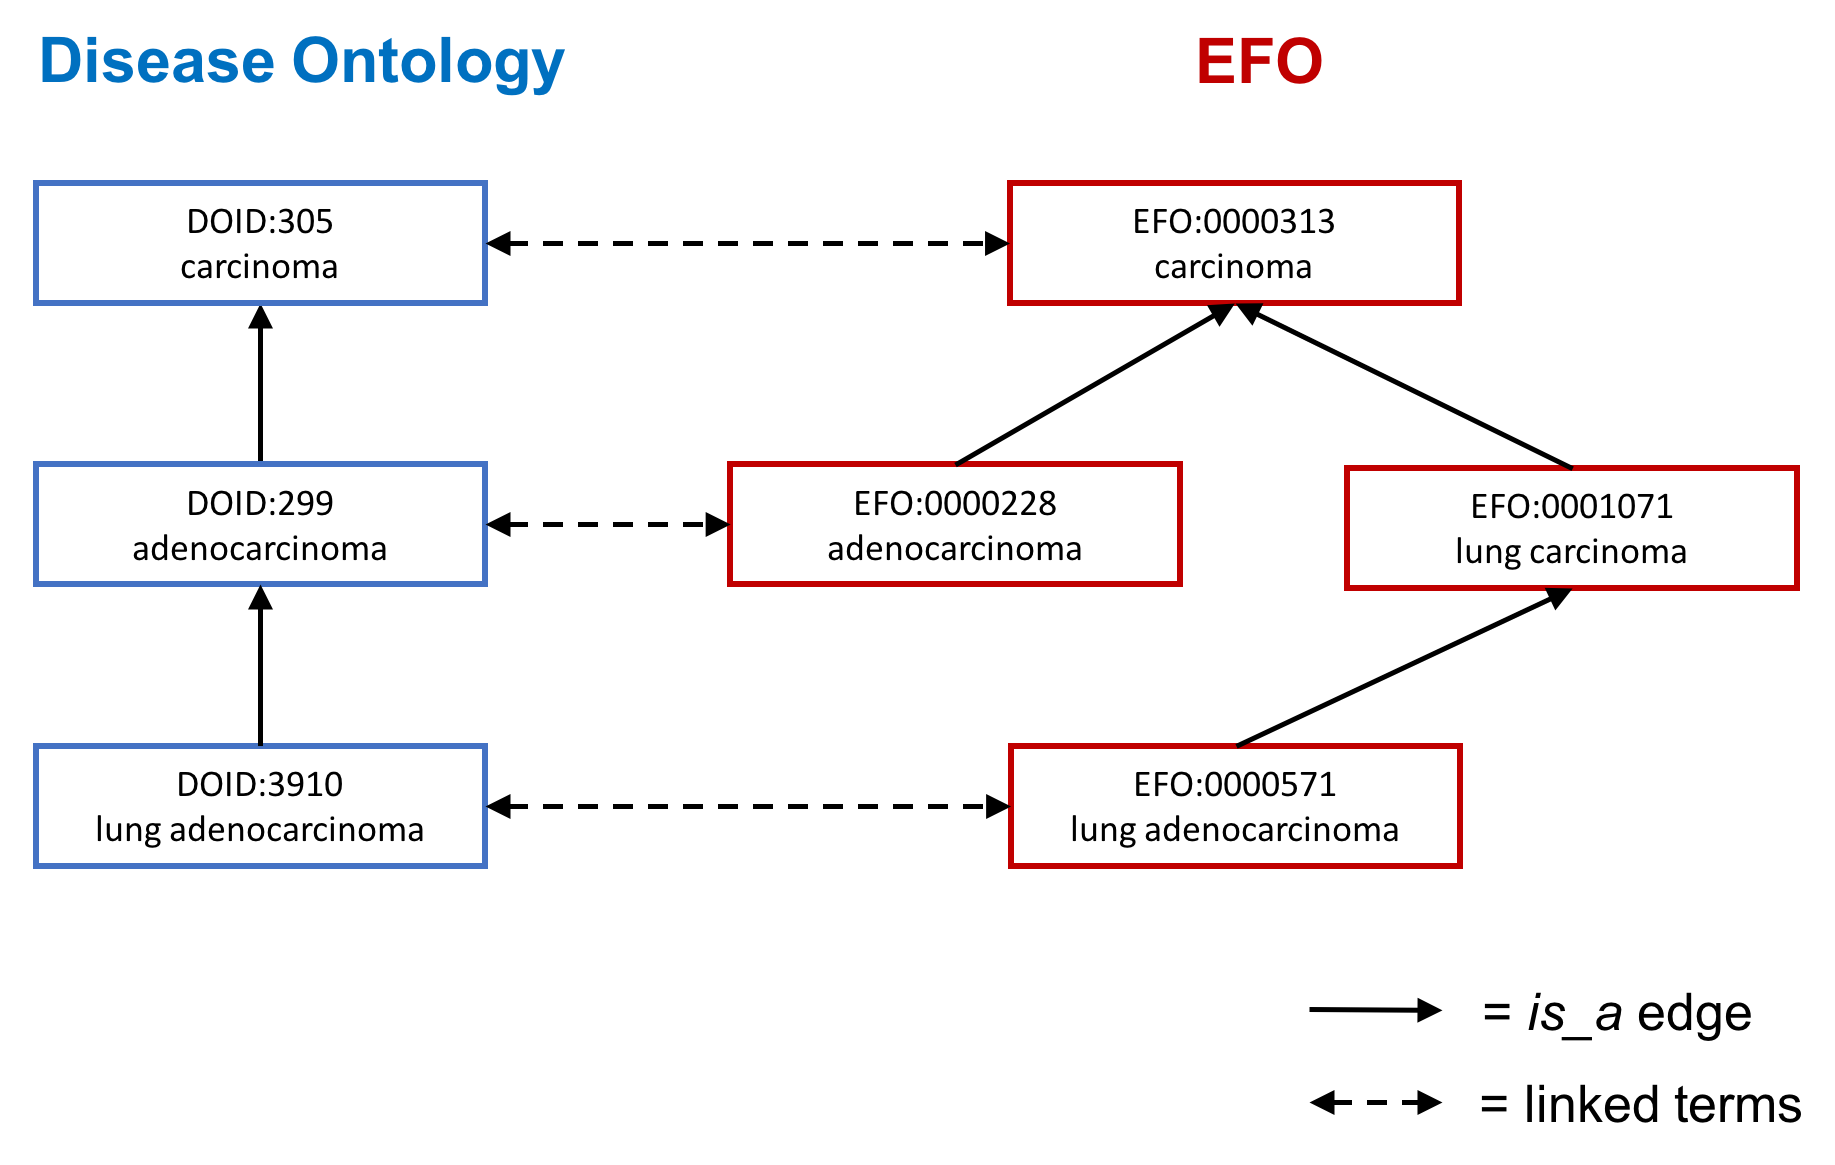
\includegraphics[scale=0.35]{figures/linked_ontologies.png} 
\caption{\textbf{Linking ontologies.} An example of linked terms between the Disease Ontology and the EFO. If a sample maps to ``lung adenocarcinoma'' in the Disease Ontology, we follow all ancestors and also map to linked terms of those ancestors. In this case, the EFO's ``adenocarcinoma'' term will also be mapped.}
\label{fig:linked}
\end{figure}

\subsection{Extracting real-value properties}
We maintain a list of ontology terms that define real-value properties. Currently, we use 6 terms: ``age'', ``passage number'', ``timepoint'', ``age at diagnosis", ``body mass index", and ``age at death."  Future work will entail expanding this list.  To extract a real-value property from a key-value pair, we search the graph emanating from the key for a match to a property ontology term.  If such a property is found, we search the graph emanating from the value for an artifact representing a numerical value and a unit ontology term node (e.g., ``46'' and ``year'').  From this process, we extract the triple (property, value, unit). For example, given the key-value pair \texttt{age: 46 years old}, we extract (``age'', 46, ``year'').

\subsection{Predicting sample-type category}\label{prediction_sample_type}

We classify samples by sample-type using a supervised machine learning approach.  This stands in contrast to the non-statistical approach used in the aforementioned ontology term mapping task. We trained a one-vs.-rest ensemble of logistic regression, binary classifiers  
%That is, each classifier learns a model of the form
%$$p(y = 1 | \bold{x}) := \left[1+\exp(\boldsymbol{\beta}^\top\bold{x})\right]^{-1}$$
%where $y=1$ indicates the sample belongs to the class, $\boldsymbol{\beta}$ are coefficients assigned to each feature, and $\bold{x}$ is the feature vector. 
where each classifier was trained using L1 regularization.  For each sample, the classifier accepts as input both the raw key-value metadata as well as the ontology terms that were mapped by our aforementioned pipeline.  The classifier then outputs the sample's predicted sample-type.

We consider two types of features for representing each sample: $n$-gram features and ontology term features.  For $n$-gram features, we consider all uni-grams and bi-grams appearing in the training samples' raw metadata.  For ontology term features, we consider the set of all ontology terms that were mapped to the training samples by our automated ontology-term mapping pipeline.  We performed a feature selection process (for details, see supplementary materials) that involved using mutual information to select features that are indicative of at least one of the target sample-types. 

When making a prediction on a sample $x$, each logistic regression binary classifier $c_j$ in the ensemble computes its estimate of the conditional probability $c_j(x) := p(y = j | x)$, which can be interpreted as the confidence that classifier $c_j$ believes that $x$ is of type $j$.  Using these probabilities, we designed a decision procedure that uses our domain knowledge for determining the sample-type.  Specifically, we limit the possible sample-types based on the ontology terms mapped to the sample. For example, if ``stem cell'' was mapped to the sample, we limit the possible predictions to \texttt{stem cells}, \texttt{induced pluripotent stem cell line}, and \texttt{in vitro differentiated cells}.  We found that injecting such domain knowledge into the process boosted performance in cross-validation experiments. See Section~\ref{sec:sample_pred} for details.  Although theoretically, the learning algorithm should learn these facts itself, there is likely not enough training examples for the algorithm to learn such patterns.

We randomly sampled and manually annotated \SampleTypeTrainingSetSize{} samples based on their metadata. We determined each sample's sample-type by consulting the sample's study, publication, and other external resources that describe the experimental procedure used to obtain the sample.  Four of these samples did not adequately fit into any sample-type category and thus were excluded from training. Since samples that belong to the same study are likely described similarly, one potential pitfall in the learning process is that if training samples are drawn uniformly and at random from all samples, the learner will be biased towards features that correlate with how larger studies describe their samples rather than features that correlate with sample-type.  To avoid this issue, we ensured that no two samples in the training set came from the same study. 




\section{Results}

\subsection{Evaluation of ontology mappings}\label{sec:eval_onto_mappings}

In order to create a test set for evaluation of our pipeline, we manually normalized metadata for \TestSetSize{} samples from the SRA where each sample belongs to a unique study. This test set was obtained by randomly sampling from entries that were recently added to the archive and had not been considered during the development of our computational pipeline. Thus, performance on this subset of data provides an unbiased estimate of its ability to generalize to unseen samples.  We note that these \TestSetSize{} samples are disjoint from the \SampleTypeTrainingSetSize{} samples described in section~\ref{prediction_sample_type} that were used to train the sample-type classifier. 

\begin{figure*}[!tpb]
\centerline{\includegraphics[width=13cm]{figures/results_fig.eps}}
\caption{\textbf{Ontology term mapping results.} (A) A schematic of an ontology subgraph demonstrating our calculation of recall, specific terms recall, error rate, and specific terms error rate.  (B) Performance of our pipeline in mapping explicit ontology terms versus BioPortal's Annotator, ZOOMA, and SORTA.  We ran SORTA using the three confidence thresholds of 1.0, 0.5, and 0.0. We also ran ZOOMA using the three confidence thresholds of high, good, and low.  We measured recall, error rate, specific terms recall, and specific terms error rate for all programs across all ontologies with the exceptions that ZOOMA only maps to three of the ontologies and only MetaSRA and SORTA map to the Cellosaurus. (C) The error rate, specific terms error rate, average retrieved terms per sample, and average specific retrieved terms per sample across all ontologies when considering only consequently mapped terms.  No terms from the Cellosaurus were consequently mapped and thus this ontology is omitted.  (D) Recall, error rate, specific terms recall, and specific terms error rate for versions of our pipeline in which certain stages are disabled.  The data points labelled ``none'' refer to the complete pipeline in which no stage is disabled.}\label{fig:results}
\end{figure*}

We first evaluated our pipeline's ability to map samples to explicitly mapped ontology terms using the following metrics: recall, error rate, specific terms recall, and specific terms error rate.  Given a sample, let $T$ be the set of all ontology terms to which the sample maps including terms ancestral to those explicitly mentioned.  Let $T'$ be the most specific terms in $T$.  That is $T' := \{t \in T : \text{no child of $t$ is in T}\}$.  Let $P$ be the set of predicted terms to which the sample maps.  Let $P'$ be the most specific terms in $P$. That is $P' := \{p \in P : \text{no child of $p$ is in P}\}$.  We define our metrics as follows: 
\begin{align*}
\text{recall} &:= \frac{|T \cap P|}{|T|}&
\text{specific terms recall} &:= \frac{|T' \cap P|}{|T'|}
\\
\text{error rate} &:=  \frac{|P \setminus T|}{|P|}&
\text{specific terms error rate} &:=  \frac{|P' \setminus T|}{|P'|}
\end{align*}
 We use these four metrics instead of traditional precision and recall because precision and recall are affected by the structure of the ontology.  This is due to the fact that the act of retrieving an ontology term implicitly retrieves all of its ancestral terms in the ontology's directed acyclic graph.  Thus, retrieving a term with a high number of ancestral terms will lead to exaggerated metrics.  The specific terms error rate corrects for this by describing the fraction of the most specific predicted terms that incorrectly describe the sample.  We note that the error rate is simply $1 - \text{precision}$.  The metrics are demonstrated in Figure~\ref{fig:results}A. 

With these metrics, we compared our pipeline to the BioPortal Annotator, SORTA, and ZOOMA across all ontologies (Fig.~\ref{fig:results}B).  Compared to these methods, our pipeline has a low error rate while maintaining a competitive recall.  For example, although the ZOOMA pipeline scores a slightly lower error rate on the Disease Ontology, Cell Ontology, and Uberon than our pipeline, this comes at the cost of a much lower recall. Similarly, although the SORTA tool scores a slightly higher specific terms recall on the Disease Ontology and Cell Ontology than our pipeline, this comes at the cost of a much higher error rate.  Lastly, we note that our pipeline scores a higher recall and lower error rate across all ontologies when compared to the BioPortal Annotator.  

We then evaluated the pipeline's ability to map consequent terms. Recall is an inappropriate metric for evaluating our ability to map consequent terms  due to the fact that the set of consequent terms is undefined.  By our definition, a consequent term is any term that the sample can be mapped to based on expert or external knowledge.  Thus, depending on the expert or external knowledge base, the set of consequent terms may change.  Furthermore, an expert may use an exceedingly large number of ontology terms to describe the sample depending on what she knows about the sample and experiment. For these reasons, we look at the total average number of consequent terms that we map to each sample.  This metric describes the amount of extra information that is provided when considering external knowledge.  We further looked at the average number of most specific mapped consequent terms.   Figure~\ref{fig:results}C displays these metrics across the ontologies.

Lastly, we evaluate the performance impact of each of our pipeline's stages, we ran our pipeline on our test set with certain individual stages disabled.  Figure~\ref{fig:results}D shows the performance impact when removing stages for filtering key-value pairs, linking ontologies, filtering sub-phrase matches,  and generating spelling and inflectional variants. As expected, the results of these tests indicate a general trade off between recall and error rate.  Certain stages may decrease recall, but pose the benefit of decreasing the error rate.  Furthermore, a given stage may be more effective for mapping terms in some ontologies rather than others.

Finally, we evaluated performance on the top 10 most commonly mapped terms.  For this analysis, we count a term as being mapped from a sample if that term is a most-specifically-mapped term for that sample.  That is, no children of the term were mapped from the sample.  For each term in the top 10 most commonly mapped terms, we sampled 100 samples at random from the entire set of samples in the MetaSRA.  For this analysis, we allowed multiple samples from the same study.  We then evaluate the precision for the target term over these 100 samples. The results are displayed in Table \ref{table:top_terms}.  These statistics provide an unbiased estimate of the precision for each term over the entire set of samples in the MetaSRA.  

    \begin{table}[h!]
    \begin{center}
    \begin{tabular}{ |c|c|c| } 
    \hline
    Term & Name & Precision \\ \hline
    CL:0000010 & cultured cell & 0.98 \\
    UBERON:0003100 & female organism & 1.00 \\
    UBERON:0003101 & male organism & 1.00 \\
    UBERON:0000955 & brain & 0.99 \\
    EFO:0000727 & treatment & 0.90 \\
    UBERON:0000178 & blood & 0.86 \\
    EFO:0003156 & Caucasian & 1.00 \\
    EFO:0000322 & cell line & 1.00 \\
    EFO:0001272 & adult & 1.00 \\
    UBERON:0007023 & adult organism & 1.00 \\
    \hline
    \end{tabular}
    \end{center}
    \caption{\textbf{Precision of the most commonly mapped ontology terms.}}
    \label{table:top_terms}
    \end{table}


\subsection{Evaluating extraction of real-value properties}

Of the \TestSetSize{} samples in our test set, \TestSetRealValSize{} described real-value properties.  We evaluated our performance in retrieving real-value property tuples in terms of precision and recall. A predicted real-value property was called a true positive if the property type, value, and unit all matched the ground truth.  On the \TestSetRealValSize{} samples, we report precision of \RealValPrecision{} and recall of \RealValRecall{}. We note that the high precision our method achieves is due to the heavy constraints we place on calling a real-value property, which also result in relatively low recall.

\subsection{Evaluating sample-type predictions}

\begin{figure*}[!tpb]
\centerline{\includegraphics[width=13cm]{figures/sample_type_prediction_results.eps}}
\caption{\textbf{Sample-type prediction results.} (A) Row-normalized confusion matrix for sample-type category prediction accuracy on the initial test data set. Element $i,j$ is the fraction of samples in category $i$ that were labelled as category $j$ by the classifier. The diagonal elements are category-specific recall values.  The number of samples in each category are shown above the matrix. (B) Transpose of the column-normalized confusion matrix for sample-type category on the enriched test data set.  Element $i, j$ represents the fraction of samples labelled as category $i$ that are truly category $j$. The diagonal elements are category-specific precision values. The number of samples predicted to be in each category are shown above the matrix.   (C) Calibration of the model.  The estimated probability of the model (average of confidence values in each bin) is plotted against the empirical probability that the model is correct (accuracy of predictions in each bin). The straight blue-line plots a well-calibrated model. Error bars are drawn according to a bootstrap sampling approach (\citealp{Brocker}). Points are omitted for bins that contain no predictions. This plot was created from the initial data set of \TestSetSize{} samples.}
\label{fig:sample_type}
\end{figure*}

To evaluate our ability to predict each sample's sample-type, we evaluated the algorithm's performance on two held-out test sets. The first test data set was created by manually annotating the sample-types for the \TestSetSize{} samples that were used for evaluating our ontology term mapping procedure.  As noted previously, no two samples in this data set belong to the same study.   We annotated all samples for which the origin of the sample was explained in an external resource such as a scientific publication. In total, this came to \NonEnrichedSampleTypeTestSetSize{} samples.  The distribution of sample-types in our test set is illustrated in the bar graph above the matrix in Figure~\ref{fig:sample_type}A.

Our trained classifier achieved an accuracy of \SampleTypeOverallAccuracy{} over these samples.  The confusion between categories is plotted in Figure~\ref{fig:sample_type}A.  In general, the classifier does well in determining the cell line samples and tissue samples.  Close inspection of the classifier's errors revealed that most were due to samples with descriptions of poor quality.  Such samples are difficult to categorize, even as a human, without consulting the scientific publication in which the sample is described. Correctly classifying these samples will require utilizing external descriptions of the samples. 

Because this test set of \TestSetSize{} samples is impoverished for some sample-types, we enriched it by sampling additional samples from each predicted sample-type category, continuing to ensure that no two samples belonged to the same study.  We sought at least 100 samples that were predicted to fall in each category; however for \texttt{primary cells}, \texttt{stem cells}, and \texttt{induced pluripotent stem cell line} samples, we were unable to achieve this threshold given our criteria. This resulted in a test data set consisting of \EnrichedSampleTypeTestSetSize{} samples.  We used this enriched test data set to better estimate the category-specific precision of our classifier (Fig.~\ref{fig:sample_type}C).  Since the sampling procedure used for the enriched test data set was biased by the predicted sample-type of each sample, it could not be used for an unbiased estimate of recall or overall accuracy.

MetaSRA includes the classifier's confidence of each prediction. To evaluate the quality of these confidence scores, we assessed the calibration of the classifier.  A classifier is well calibrated if for any instance $x$ with true label $y$, it holds that $\hat{p} = p(\hat{y} = y)$ where $\hat{y}$ is the classifier's predicted class label of $x$ and $\hat{p}$ is its confidence. To assess calibration, we grouped the predictions  into bins according to their confidence scores and compute the empirical accuracy of predictions in each bin (Fig.~\ref{fig:sample_type}B).  We found the classifier to be well calibrated, and thus that its confidence scores may be of use in filtering predictions to a achieve a target accuracy level.

We note that the test data set was small compared to the training data set. To provide an estimate of the performance of the classifier on a larger data set, we ran the algorithm using leave-one-out cross validation on the training set. The algorithm achieved 0.845 accuracy on this data set.  Figure~\ref{fig:train_set}A shows the row-normalized confusion matrix and Figure~\ref{fig:train_set}B shows the calibration of the model.

\begin{figure}[htbp]
\centering
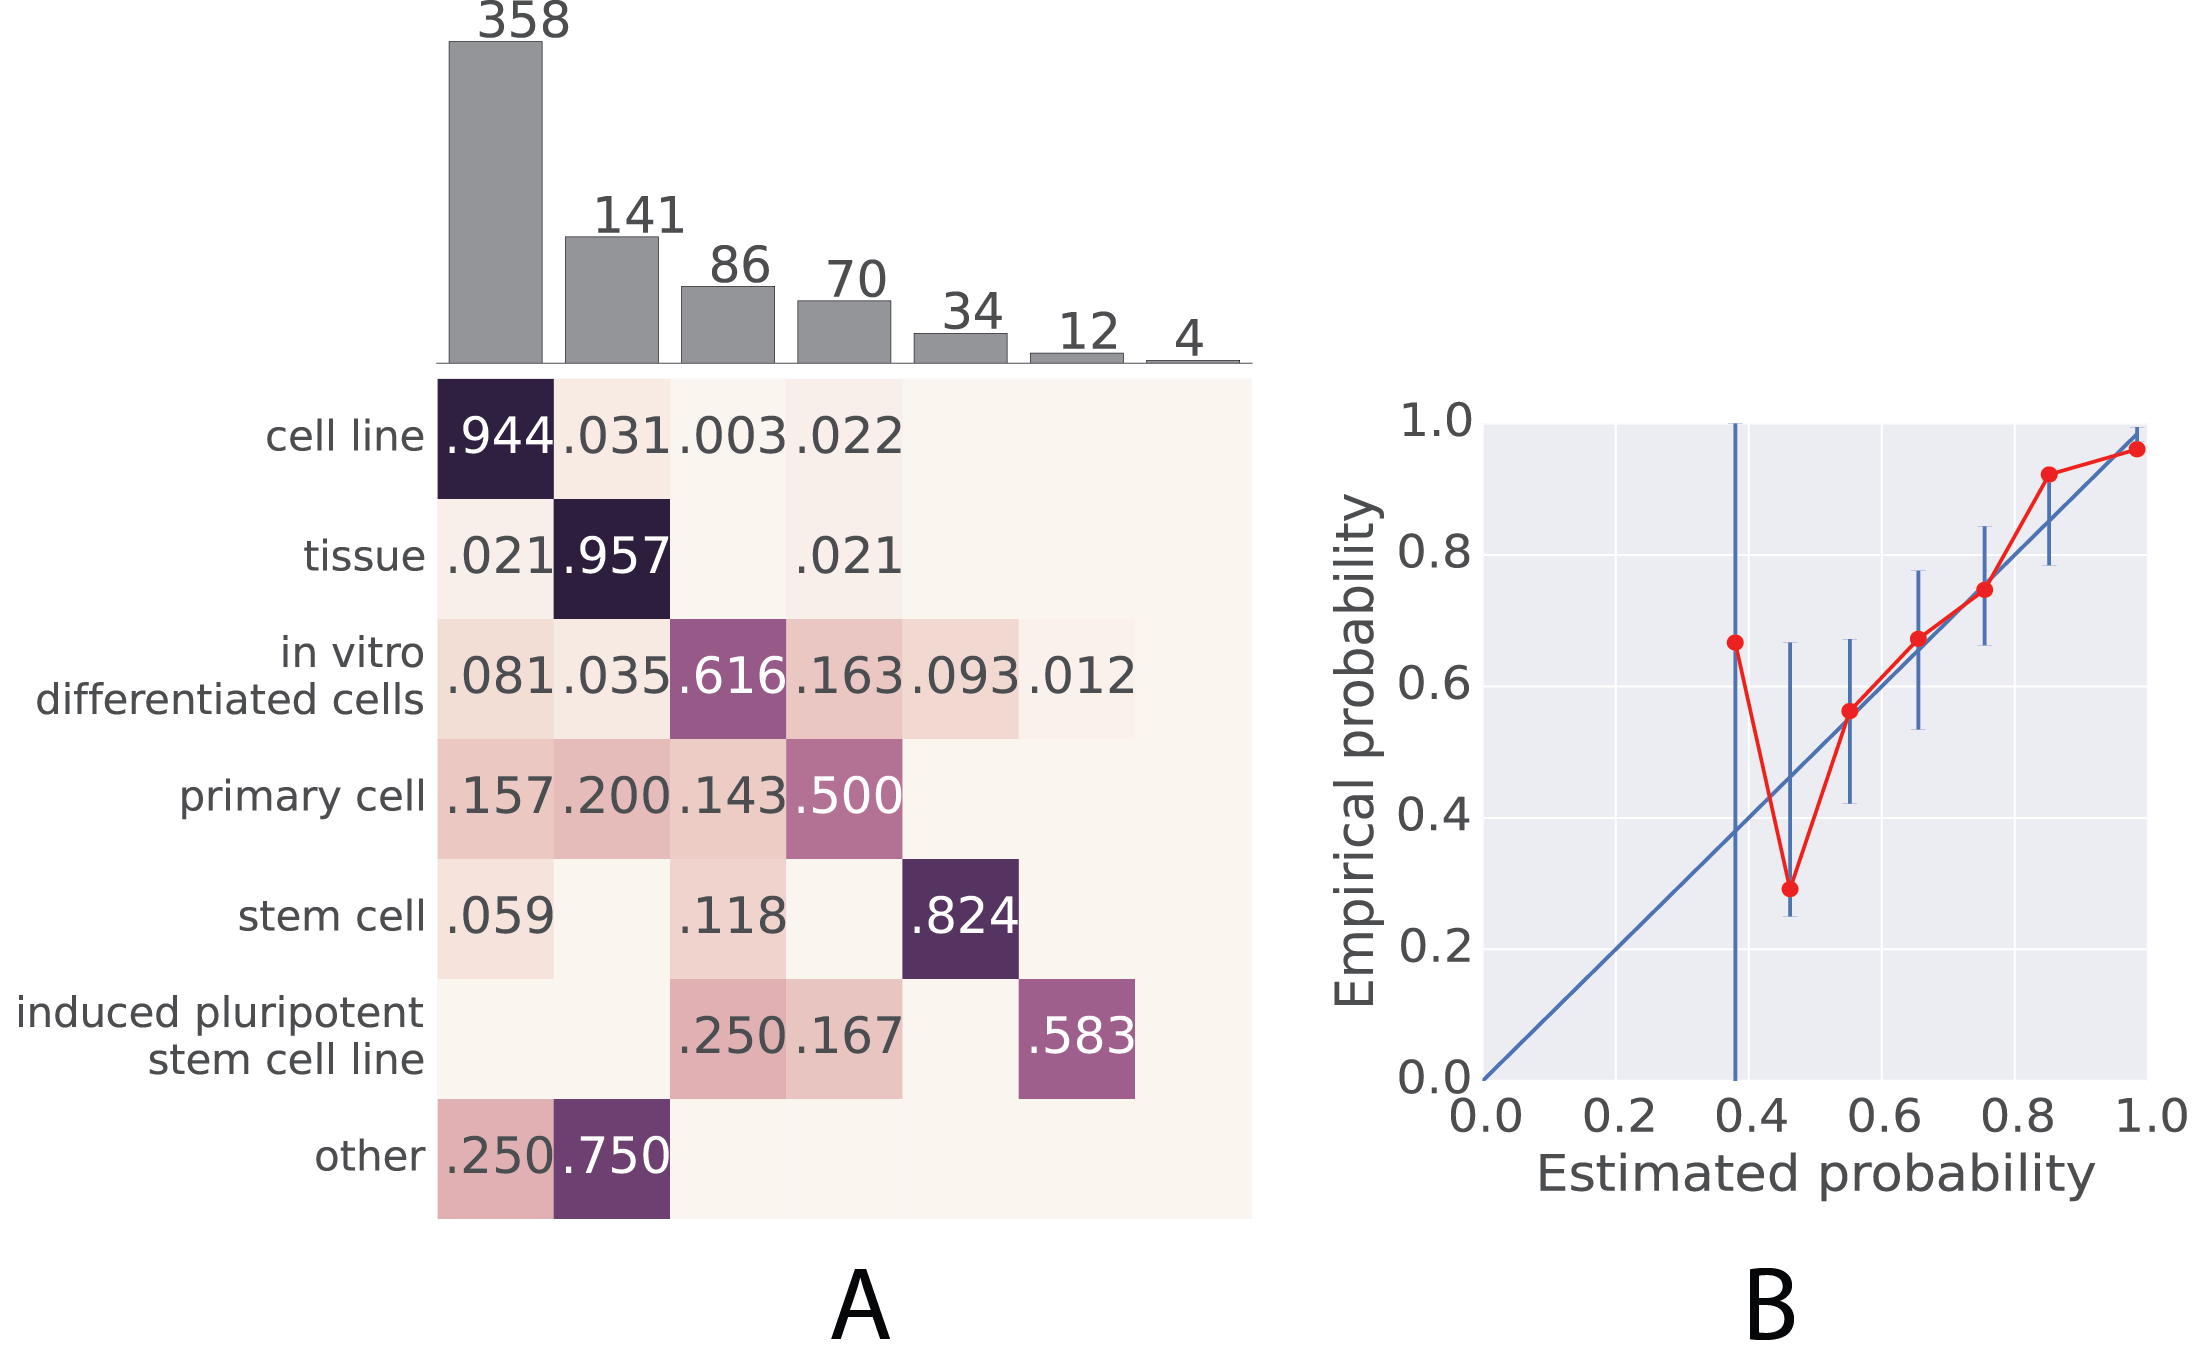
\includegraphics[width=13cm]{figures/sample_type_training_set.png} 
\caption{\textbf{Sample-type prediction results on the training set.} (A) The confusion matrix of the algorithm on the training set evaluated using leave-one-out cross validation. The bar graph above the matrix displays the distribution of classes within the training set. (B) Plotting the calibration of the classifier.}
\label{fig:train_set}
\end{figure}


\subsection{Summarizing the MetaSRA}\label{sec:sum_metasra}

We summarized the contents of the MetaSRA run on all samples, including those that belong to the ``large'' ($\geq 100$ samples) studies.  First, we explored the distribution of the number of samples mapped to each ontology term (Fig.~\ref{fig:metasra_summary}A).  Most terms from each ontology map to fewer than 100 samples, whereas a few terms map to upwards of 10,000 samples.  Second, we looked at the fraction of samples that were mapped to terms within each ontology (Fig.~\ref{fig:metasra_summary}B).  The fraction of samples mapping to each ontology differed markedly between samples of different predicted sample type, which provides some insight into how the sample-type classifier makes its decisions.  For example, tissue samples tend to be described by an anatomical term in the Uberon ontology and not described by a specific cell type in the Cell Ontology. 
Lastly, we identified the most common ontology terms (Fig.~\ref{fig:metasra_summary}C) 
%and real value properties (Table~\ref{tab:real_val_props})
in the MetaSRA.  In general, the error rate for the most common ontology terms was quite low.

\begin{figure*}[!tpb]
\centerline{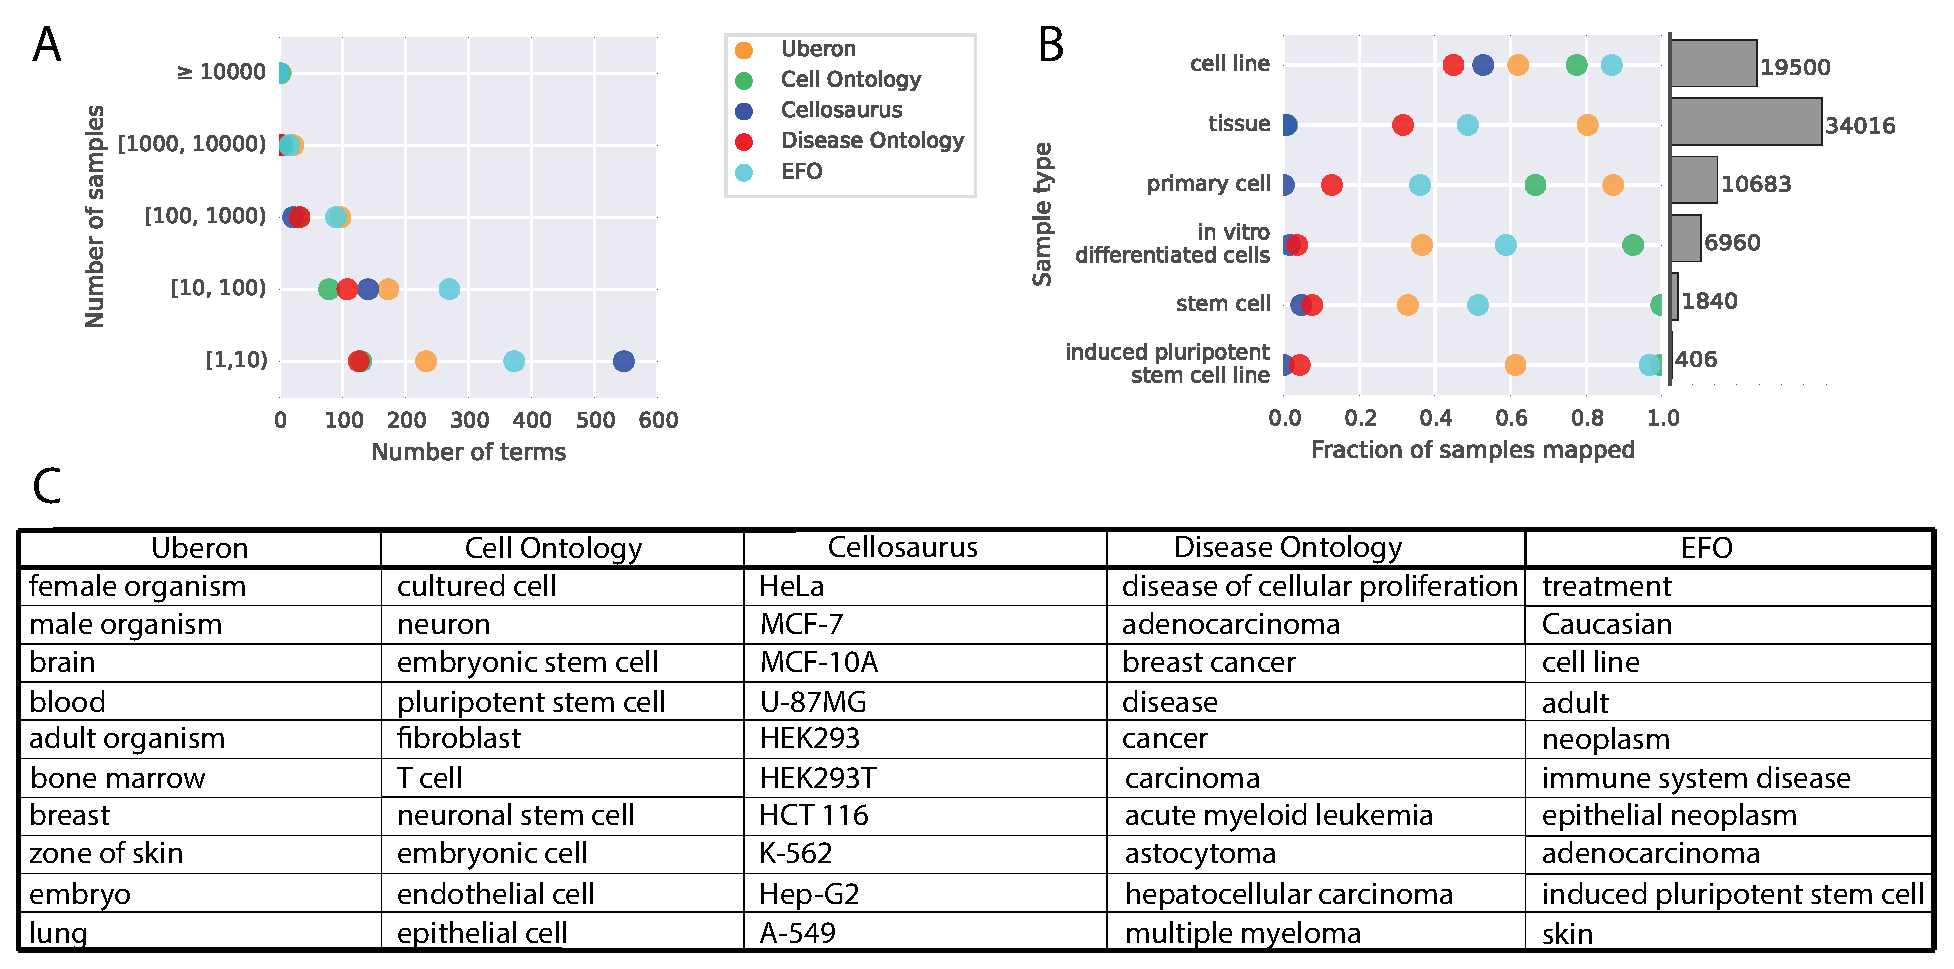
\includegraphics[width=13cm]{figures/metasra_summary.eps}}
\caption{\textbf{Summary of the MetaSRA.} (A) The number of terms from each ontology that map to a given range of number of samples.  Only the most-specifically mapped terms for each sample are considered. (B) Fraction of samples of each predicted sample-type that map to each ontology. The bar plot to the right of the strip-plot shows the number of each predicted sample-type. (C) The most commonly mapped terms for each ontology. Only the most-specifically mapped terms for each sample are considered.}
\label{fig:metasra_summary}
\end{figure*}

%\begin{table}[!th]
%\processtable{The number of samples in the MetaSRA that are annotated with each real-value property. Overall, \PercentageMetaSRARealVal{}\% of samples were mapped to a real-value property.\label{tab:real_val_props}} {\begin{tabular}{@{}lll@{}}\toprule
%Property & Number of samples & Percentage of samples \\ \midrule
%        age & 12416 & 16.9 \\
%passage number & 3307 & 4.5 \\
%timepoint & 831 & 1.1 \\
%age at diagnosis & 645 & 0.9 \\
%body mass index & 200 & 0.3 \\
%age at death & 98 & 0.1 \\
%\botrule
%\end{tabular}}{}
%\end{table}






























\chapter{Hierarchical cell type classification using mass, heterogeneous RNA-seq data from human primary cells} \label{chap:2}

The work in this chapter is available as a preprint on bioRxiv (\citealp{Bernstein2019}). 

\section{Background}

Gene expression-based computational classification of a biological sample's constituent cell type is an important task in many gene expression analysis tasks including that of annotating cell types in single-cell RNA-seq datasets (\citealp{Alavi2018, Lin2017}), improving the metadata in public genomic databases (\citealp{Lee2013, Ellis}), and verifying outcomes of experiments that entail inducing cellular differentiation (\citealp{Cahan, Radley2017}).  Furthermore, interpretable cell type classifiers may enable greater understanding of cell-type-specific expression patterns and may prove useful towards efforts, such as the Human Cell Atlas (\citealp{Regev2017}), that seek to define and catalog all cell types in the human body.  The NCBI's Sequence Read Archive (SRA) (\citealp{Leinonen2011}) promises to be a valuable resource for training machine learning algorithms for this task due to the high number and large variety of cell type samples it contains.   However, it has remained underutilized due to both the poor structure of the metadata (\citealp{Goncalves2017}) and the difficulty in obtaining uniformly processed expression data. These challenges have recently been addressed through efficient RNA-seq quantification algorithms (\citealp{Patro2017, Bray2016}) and the metadata normalization efforts discussed in Chapter~\ref{chap:1}, thus paving the way towards the utilization of the SRA for training cell type classifiers. 

In this work, we address three goals pertinent to this task:
\begin{enumerate}
    \item To capture robust cell type signals by training on, and evaluating with, only healthy, primary, purified human samples.
    \item To take advantage of the hierarchical nature of cell type definitions by exploring novel applications of hierarchical machine learning classification methods.
    \item To build interpretable models that can be used to gain deeper understanding into the expression patterns that distinguish cell types.
\end{enumerate}
Existing approaches for cell type prediction address some of these goals, but there has yet to be an investigation that addresses them all simultaneously. 

First, to the best of our knowledge, none of the existing machine learning-based cell type classification approaches that train on public expression data distinguish between treated versus untreated cells (\citealp{Alavi2018, Cahan, Lee2013}). By training on non-primary cells or treated cells, a classifier becomes more susceptible to batch effects when treatment or disease confounds cell type. This also leads to difficulty in model interpretation as it is unclear whether the derived signal is indicative of cell type or of a confounding variable such as treatment or disease. In this work, we compiled a set of training data from the SRA comprising only healthy, primary cells.

We also assert that framing the cell type classification task as that of \textit{multi-label, hierarchical classification} against the Cell Ontology (\citealp{Bard}) poses a number of advantages over flat-classification. The Cell Ontology provides a comprehensive hierarchy of animal cell types encoded as a directed acyclic graph (DAG). This DAG provides a rich source of prior knowledge to the cell type classification task that remains un-utilized in flat classification.

Flat classification suffers from the possibility that predictions are logically inconsistent with the hierarchy of cell types in that the classifier for some cell type may, for a given query, output a probability that is larger than the classifier's output for its parent cell type in the hierarchy (\citealp{Obozinski2008}). Such outputs reduce the interpretability, and therefore scientific usefulness, of the model.  In addition, the use of hierarchical classification approaches allows for the placement of a bulk RNA-seq sample at a level of the hierarchy appropriate to its heterogeneity. For example, a population of cells enriched for T cells may be heterogeneous in the sub-types of T cells (e.g., CD4+ T cells and CD8+ T cells).  

In regards to classification of scRNA-seq data, hierarchical classification allows for informative predictions to be made on query samples whose true phenotype label may not be included in the ontology either because the ontology is incomplete or that phenotype has yet to be discovered. Finally, by utilizing the hierarchy during training rather than using flat classification, more accurate classifiers can be learned (\citealp{BarutcuogluSchapireTroyanskaya2006}). 

To the best of our knowledge, only work by  \cite{Kanter2019} and \cite{Lee2013} frames the cell type prediction task as a hierarchical classification problem.  \cite{Kanter2019} developed an algorithm called CHETAH that learns a hierarchy from the training data; however, this algorithm does not take advantage of the rich hierarchy of cell types already available in biomedical ontologies.  \cite{Lee2013} developed an algorithm called URSA that does utilize a pre-existing ontology of tissues and cell types, and to this end, train a hierarchical classifier using Bayesian Network Correction (BNC) (\citealp{BarutcuogluSchapireTroyanskaya2006}). However, there also exist discriminative methods for hierarchical classification that have yet to be applied to the cell type prediction task. Thus, we applied a number of such approaches including cascaded logistic regression (CLR), isotonic regression correction (IR) (\citealp{Obozinski2008}), and a heuristic procedure called the True Path Rule (TPR) (\citealp{Notaro2017}). We compared these discriminative methods to BNC and in our hands found them to outperform the BNC approach.

Furthermore, we sought for our methods to be interpretable in order for our trained classifiers to be of use not only in classification, but also for investigating cell type-specific expression patterns. To this end, this work makes extensive use of linear models, which are particularly amenable to interpretation. We tested the interpretability of the aforementioned frameworks and found that CLR is particularly interpretable as it is able to delineate functional differences between similar cell types.

We tested these algorithms on single-cell RNA-seq (scRNA-seq) data, resulting in promising performance. We propose that hierarchical, machine learning-based classification of single-cell expression data will help overcome a number of challenges in cell type labeling of single-cell datasets.  Currently, labeling cell types in scRNA-seq data is an ad hoc process that involves clustering the cells and then searching for differential expression of certain cell-type-specific marker genes across these clusters. This process is challenged both by the fact that there is not a canonical set of marker genes for most cell types (\citealp{Zhang2018}) and that this process is affected by the clustering algorithm (\citealp{Kiselev2019}). Approaches are beginning to emerge that rely on training cell type classifiers on single-cell data (\citealp{Xie2019, Alavi2018}).  

We note that the process of training a cell type classifier on single-cell data is somewhat circular in that the ground truth cell type labels are most commonly based upon gene expression (via the expression of cell type-specific marker genes), which is then also used for constructing the machine learning features.  In this work, we train our algorithms on only bulk RNA-seq data, that originate from cells that have been isolated based on phenotypic characteristics downstream of gene expression itself (such as cell surface proteins). Thus, we suggest that bulk RNA-seq data in the SRA cannot only be utilized, but also may be preferred, for the training of cell type classifiers applied towards scRNA-seq datasets. 

Finally, we created a Python package, CellO (\textit{Cell} \textit{O}ntology-based classification) that allows users to run pre-trained classifiers on their own RNA-seq data. CellO is available at \ClassifierURL{}.

\section{Results and discussion}

\subsection*{A novel curated RNA-seq dataset of human primary cells}\label{sec:primary_cell_data}

In order to capture robust cell type signals, we sought a dataset of RNA-seq samples comprising only healthy primary cells. We did not wish to include cells that underwent multiple passages, were diseased, or underwent other treatments, such as in vitro differentiation, because these conditions alter gene expression. We therefore curated a novel dataset from the SRA consisting of healthy, untreated, primary cells.  We leveraged the annotations provided by the MetaSRA, which includes sample-specific information including disease-state, treatment, and sample type (i.e., their status as primary cells). Consequently, we followed the conservative definition for a primary cell sample according to the criteria laid out in Chapter~\ref{chap:1}, which requires that a sample has not undergone passaging beyond the first culture.  We used the MetaSRA to capture an initial candidate set of primary samples and then within this set, manually annotated these samples for technical variables (such as bulk vs. single-cell status) by consulting sources of metadata that are not captured by the MetaSRA annotation process such as fields in Gene Expression Omnibus (\citealp{Barrett2013}) records and each study's publication.  When found, we corrected errors in the MetaSRA-provided Cell Ontology labels. 

This process resulted in a dataset comprising \TotalExperiments{} total samples.  We uniformly quantified and normalized (via log counts per million) gene expression from the raw RNA-seq data for these samples.  Of these samples, \ExperimentsInBulkDataset{} were bulk RNA-seq samples from \StudiesInBulkDataset{} studies and labeled with \CellTypesInBulkDataset{} cell type terms in the Cell Ontology. Of these cell types, \MostSpecificBulkCellTypes{} cell types were the most-specific cell types in our dataset (i.e., no sample in our data was labelled with a descendent cell type term). These cell types were diverse, spanning multiple stages of development and differentiation (Fig.~\ref{fig:dataset_summary}). To the best of our knowledge, this dataset is the largest and most diverse set of bulk RNA-seq samples derived from only primary cells.  Prior to this work, the most comprehensive bulk primary cell transcriptomic dataset was compiled by Aran \textit{et al.} (2017), which contained data for 64 cell types from 6 studies.  Whereas our dataset consists of only RNA-seq data, this prior dataset included samples assayed with several other technologies, such a microarrays.  In addition to bulk samples, our dataset also includes \ExperimentsInSingleCellDataset{}  single-cell samples from \StudiesInSingleCellDataset{} studies and labeled with \CellTypesInSingleCellDataset{} cell types. We note that this data includes single-cell samples from protocols such as MARS-seq (\citealp{Jaitin2014}) and SMART-Seq2 (\citealp{Picelli2013}), but it does not include data from droplet-based protocols such as Chromium 10x. Chapter~\ref{chap:3} will address cell type prediction on RNA-seq generated from these more novel technologies.


\clearpage
 \begin{sidewaysfigure}
    \thispagestyle{empty}
    %\vspace{-4.5cm}
    \centerline{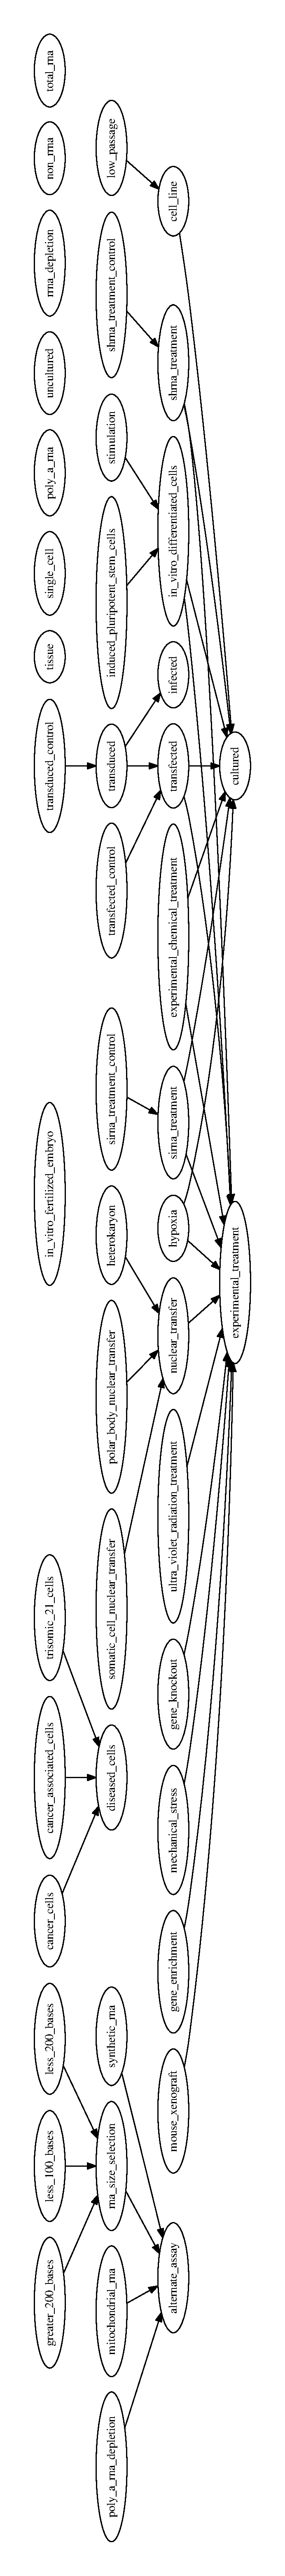
\includegraphics[scale=0.24, angle=-90]
    {figures/tags.pdf}}
    \caption{\textbf{Custom technical label graph.} We created a custom hierarchy of technical variables, in the form of a directed acyclic graph, in order to annotate the technical variables in the retrieved RNA-seq samples. Edges in the graph indicate an ``is a" relationship between terms.  We partitioned and filtered the candidate set of primary cell samples based on their labels within this technical variables hierarchy.  For example, we created separate bulk and single-cell RNA-seq datasets. In addition, we used this hierarchy to exclude any samples for which the RNA underwent size-selection, that were associated with disease, or treated.  We did, however, choose to include those samples that were treated with a ``control" treatment (e.g., labelled with ``transformed\_control").  Our inclusion criteria removed any samples that underwent multiple passages in culture or were induced into in vitro differentiation or activation.}
    \label{fig:tech_labels}
      \end{sidewaysfigure} 

  \begin{figure}[h!]
    \centerline{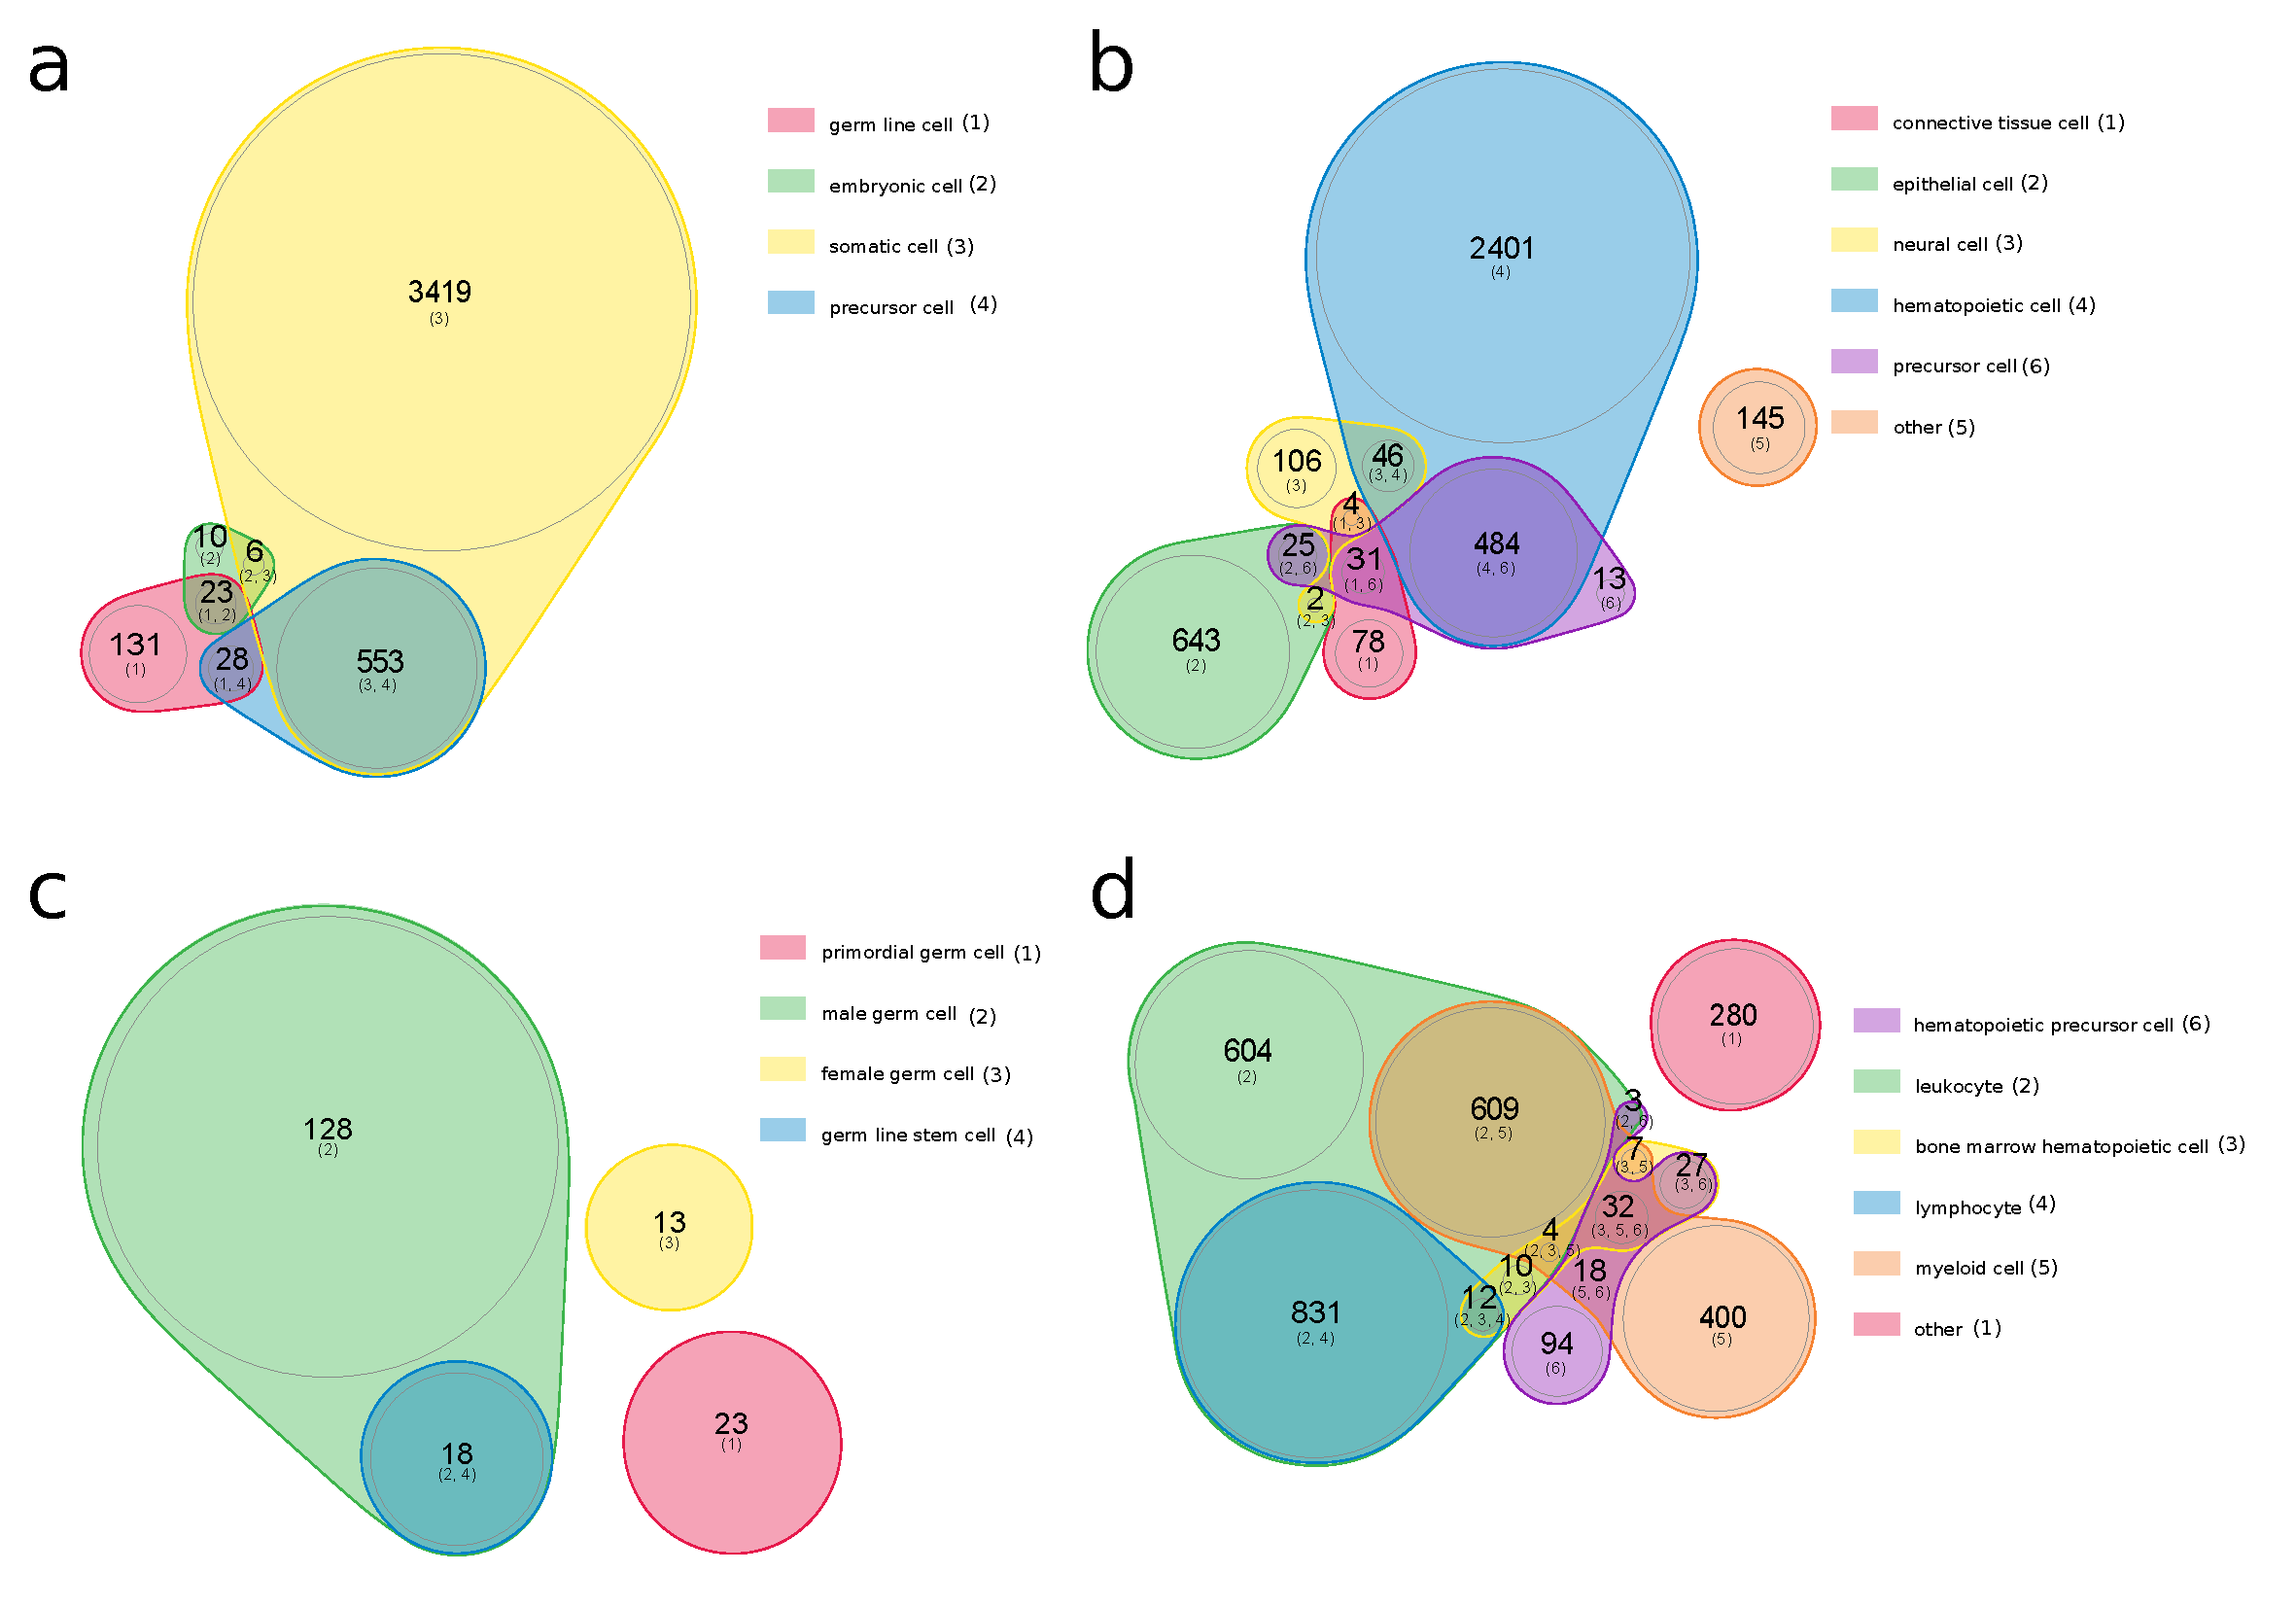
\includegraphics[width=13cm]{figures/data_venn.pdf}}
    \caption{
      \textbf{Primary cell dataset summary.} Euler diagrams of the cell types in the bulk RNA-seq data set divided by (\textbf{a}) broad cell types, (\textbf{b}) somatic cell types, (\textbf{c}) germ line cell types, and  (\textbf{d}) hematopoietic cell types. Diagrams were created with nVenn (\citealp{PerezSilva2018}). }
    \label{fig:dataset_summary}
      \end{figure}

To evaluate the implemented machine learning methods on their ability to classify bulk RNA-seq data, we split the bulk RNA-seq data set into a training and a test set, ensuring both that samples from the same study were never split across the training and test sets and that the training and test partitions had a high overlap of cell types. This partition yielded a training set with \ExperimentsInBulkTrainingDataset{} samples across \StudiesInBulkTrainingDataset{} studies and a test set with \ExperimentsInBulkTestDataset{} samples across \StudiesInBulkTestDataset{} studies. The training set and test set shared \NumCellTypesIntersectTrainingTest{} cell types. 

We separately evaluated these methods on their ability to classify scRNA-seq data. To this end, we created a second test set of all single-cell samples whose cell types appeared in the bulk RNA-seq data. This resulted in a test set of \BulkRestrictedSingleCellExperiments{} samples across \BulkRestrictedSingleCellStudies{} studies from \BulkRestrictedSingleCellCellTypes{} cell types. As detailed below, we separately examined how the classifiers handled the remaining single-cell samples whose cell types do not appear in the bulk RNA-seq training data.

\subsection*{Novel applications of hierarchical classification methods}

One straightforward approach to performing cell type prediction against the Cell Ontology entails training an independent binary classifier for each cell type in the ontology.  We will refer to this as the ``independent classifiers'' approach.  Such an approach suffers from the possibility that the classifiers' outputs will be inconsistent with the hierarchical structure of the ontology. An inconsistency occurs when the output probability for a given cell type exceeds that of one of its parent cell types in the ontology. We tested the use of independent classifiers and found inconsistencies to be an important source of errors. Specifically, we trained independent, one-vs.rest cell type classifiers on the bulk RNA-seq training set, applied them to the test set, and then examined the consistency of all edges that were adjacent to at least one cell type whose classifier produced a non-negligible probability ($> 0.1$) of the sample originating from that cell type (Fig.~\ref{fig:cdf_incons}).  Of these edges, \FracEdgesInconsistent{} were inconsistent.

\begin{figure}[htbp]
    \centerline{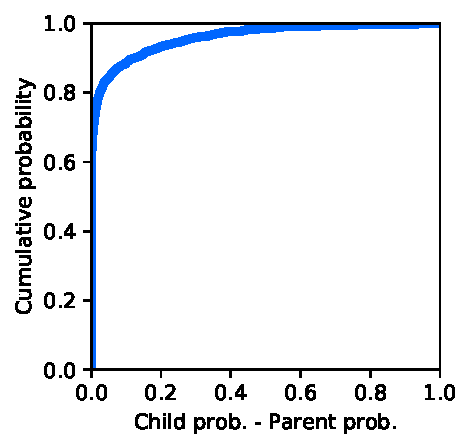
\includegraphics[scale=1.0]{figures/CDF_inconsistences.pdf}}
    \caption{\textbf{Distribution of edge inconsistencies.} The cumulative distribution function over the difference in probability between the parent and child classifiers for all edges for which either the parent or child classifier output a probability greater than 0.01.  A total of \EdgesSeverelyInconsistent{} edges saw a difference in probability greater than 0.5 which constitutes approximately one severely inconsistent edge for every ten samples.}
    \label{fig:cdf_incons}
      \end{figure} 

Hierarchical classification algorithms ensure that the output probabilities are consistent with the ontology. We tested three ensemble-based hierarchical classification algorithms that have yet to be applied to the gene expression-based cell type prediction task: cascaded logistic regression (CLR), isotonic regression correction (IR) (\citealp{Obozinski2008}), and a heuristic procedure called the True Path Rule (TPR) (\citealp{Notaro2017}). Cascaded logistic regression entails classifying a sample in a top-down fashion from the root of the ontology downward via an ensemble of binary classifiers. Specifically, each binary classifier is associated with a cell type and is trained to classify a sample conditioned on the sample belonging to all of the cell type's parents in the ontology. In contrast, IR and TPR train independent, unconditional, one-versus-rest binary classifiers for each cell type and then, for a given query sample, reconcile the output of these independent classifiers to be consistent with the ontology. IR uses a projection-based approach for reconciliation, that entails finding a set of consistent output cell type probabilities that minimize the sum of squared differences to the raw, and possibly inconsistent, classifier output probabilities. In contrast, TPR uses a heuristic procedure that involves a bottom-up pass through the ontology such that the output of children classifiers are averaged with the output of the parent classifier to allow information flow across the ontology graph.

To date, the one hierarchical classification method that has been applied to the task at hand is BNC (\citealp{BarutcuogluSchapireTroyanskaya2006}), and therefore, as a baseline, we implemented a BNC algorithm following the description in \cite{Lee2013}.  We tested a number of variants of this algorithm and report here the best-performing variant (Fig.~\ref{fig:bncvariants}).  Lastly, as a na\"ive baseline, we implemented a one-nearest-neighbor algorithm that simply returns the cell type labels of the most similar sample in the training set to the query sample using Pearson correlation as the similarity metric.  

\begin{figure}[htbp]
    \centerline{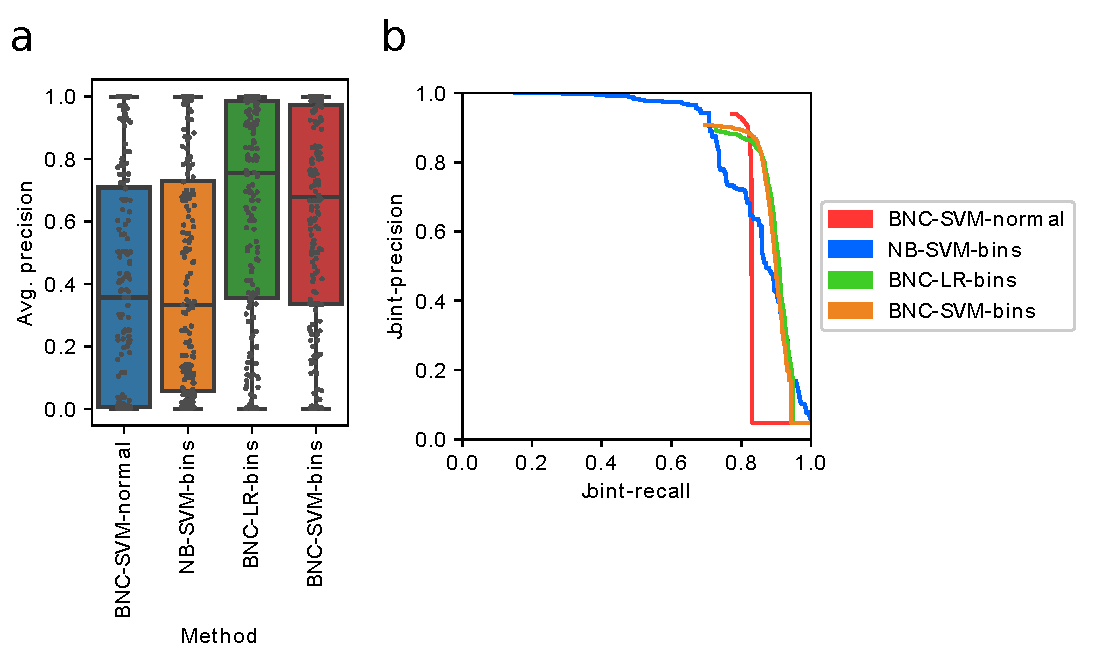
\includegraphics[width=13cm]{figures/bulk_test_bnc_results.pdf}}
    \caption{\textbf{Performance of BNC variants.} Analysis of four variants of the BNC algorithm on the bulk RNA-seq test set.  We compared a variant that uses normal distributions instead of bins (BNC-SVM-normal), a naive Bayes algorithm (NB-SVM-bins), and a variant that uses logistic regression instead of SVMs (BNC-LR-bins) to the approach used in the paper (BNC-SVM-bins). We compared these methods using the per-cell type mode of evaluation in which we compare the distributions of cell type average precision scores (a) as well as the joint mode of evaluation in which we compare the joint precision-recall curves (b).}
    \label{fig:bncvariants}
      \end{figure}

We performed three modes of evaluation: per-cell-type, per-sample, and joint (\citealp{Obozinski2008}). In the per cell type mode of evaluation we evaluate the performance of each method on each cell type independently. The results of this mode of evaluation are provided for users who are interested in examining each method's performance on specific cell types. Specifically, for each cell type, we compute both the average precision (a measure of the area under the precision-recall curve) as well as the maximum achievable recall at 0.9 precision. This latter metric is provided for users who cannot tolerate low precision. 

In the per-sample mode of evaluation, we examine the average performance of the classifiers on a per-sample basis.  To this end, we used two variants of precision and recall that are sample-centric. Given a sample, the first variants are the standard precision and recall over the sample's true cell types and predicted cell types. The second variants, which we call \textit{specific-precision} and \textit{specific-recall}, take into account only the sample's most-specific true cell types and predicted cell types according to the ontology (i.e., the deepest terms in the ontology -- see Methods).  Then, for a given prediction threshold, we compute the mean precision and recall (as well as mean specific-precision and mean specific-recall) across all samples. By varying our prediction threshold, we compute a \textit{mean precision-recall curve}, where an operating point on this curve describes an achievable mean precision and mean recall across all samples. 

A disadvantage to these mean precision and mean recall metrics is that they can be dominated by large studies due to samples from the same study sharing batch effects and similar cell type labels. To counteract this, we also compute curves in which in our calculation of the mean precision and mean recall at a given threshold down-weights samples according to the number of samples in its study in order to ensure that each study contributes equally to the mean precision-recall curve. We refer to these curves as \textit{study-weighted, precision-recall curves}. An operating point on such a curve describes an expected precision and recall that is achievable given that a study is first sampled uniformly from all available studies, and then an RNA-seq sample is sampled uniformly from that study. 

Lastly, for each method, we performed a joint evaluation that entailed treating each paired sample and cell type prediction independently. The set of all such predictions was ordered according to prediction probability and the corresponding precision-recall curve was constructed.

\subsection*{Advantages of training on data from heterogeneous sources}

We hypothesized that by leveraging data from multiple studies, we could mitigate the models fitting a single study's batch effects, and would therefore learn more robust signals for each cell type.  We tested this hypothesis using a flat classification experimental setup in which the hierarchy of cell types was first ignored.  Specifically, for a variety of cell types, we compared the performance between logistic regression binary classifiers trained on homogeneous data (data originating from a single study) versus those trained on heterogeneous data (data originating from different studies). 

The experiment proceeded as follows: we first queried the bulk RNA-seq data for all cell types that included at least three studies with over 10 experiments for that cell type. For each of these cell types, $c$, we partitioned the data labelled with $c$ according to their study of origin, and then iteratively held out each study-partition as a test set. From the remaining held-in partitions, we constructed two sets of training sets. The first set of training sets included positive examples (i.e. data labeled with $c$) from only one study, which we call \textit{homogeneous training sets}. The second set of training sets included positive examples from all held-in study-partitions, which we call the \textit{heterogeneous training sets}. For all training sets, we use a consistent set of negative examples randomly chosen from the samples that are not labelled as $c$.  Furthermore, when constructing each training set, we ensured each had an equal number of positive examples. We then trained a binary classifier on each training set and evaluated them on the held-out study-partition. Figure~\ref{fig:homo_vs_hetero_setup}a provides a schematic of the experiment (See Supplementary Materials for full details).  We computed the mean average-precision for the homogeneously trained and heterogeneously trained classifiers across each held out study-partition and cell type pair and  found that heterogeneously trained classifiers tended to have a higher mean average precision (Fig.~\ref{fig:homo_vs_hetero_setup}b).  These results support the hypothesis that better generalization can be achieved by training on data from multiple studies.

  \begin{figure}[h!]
  \centerline{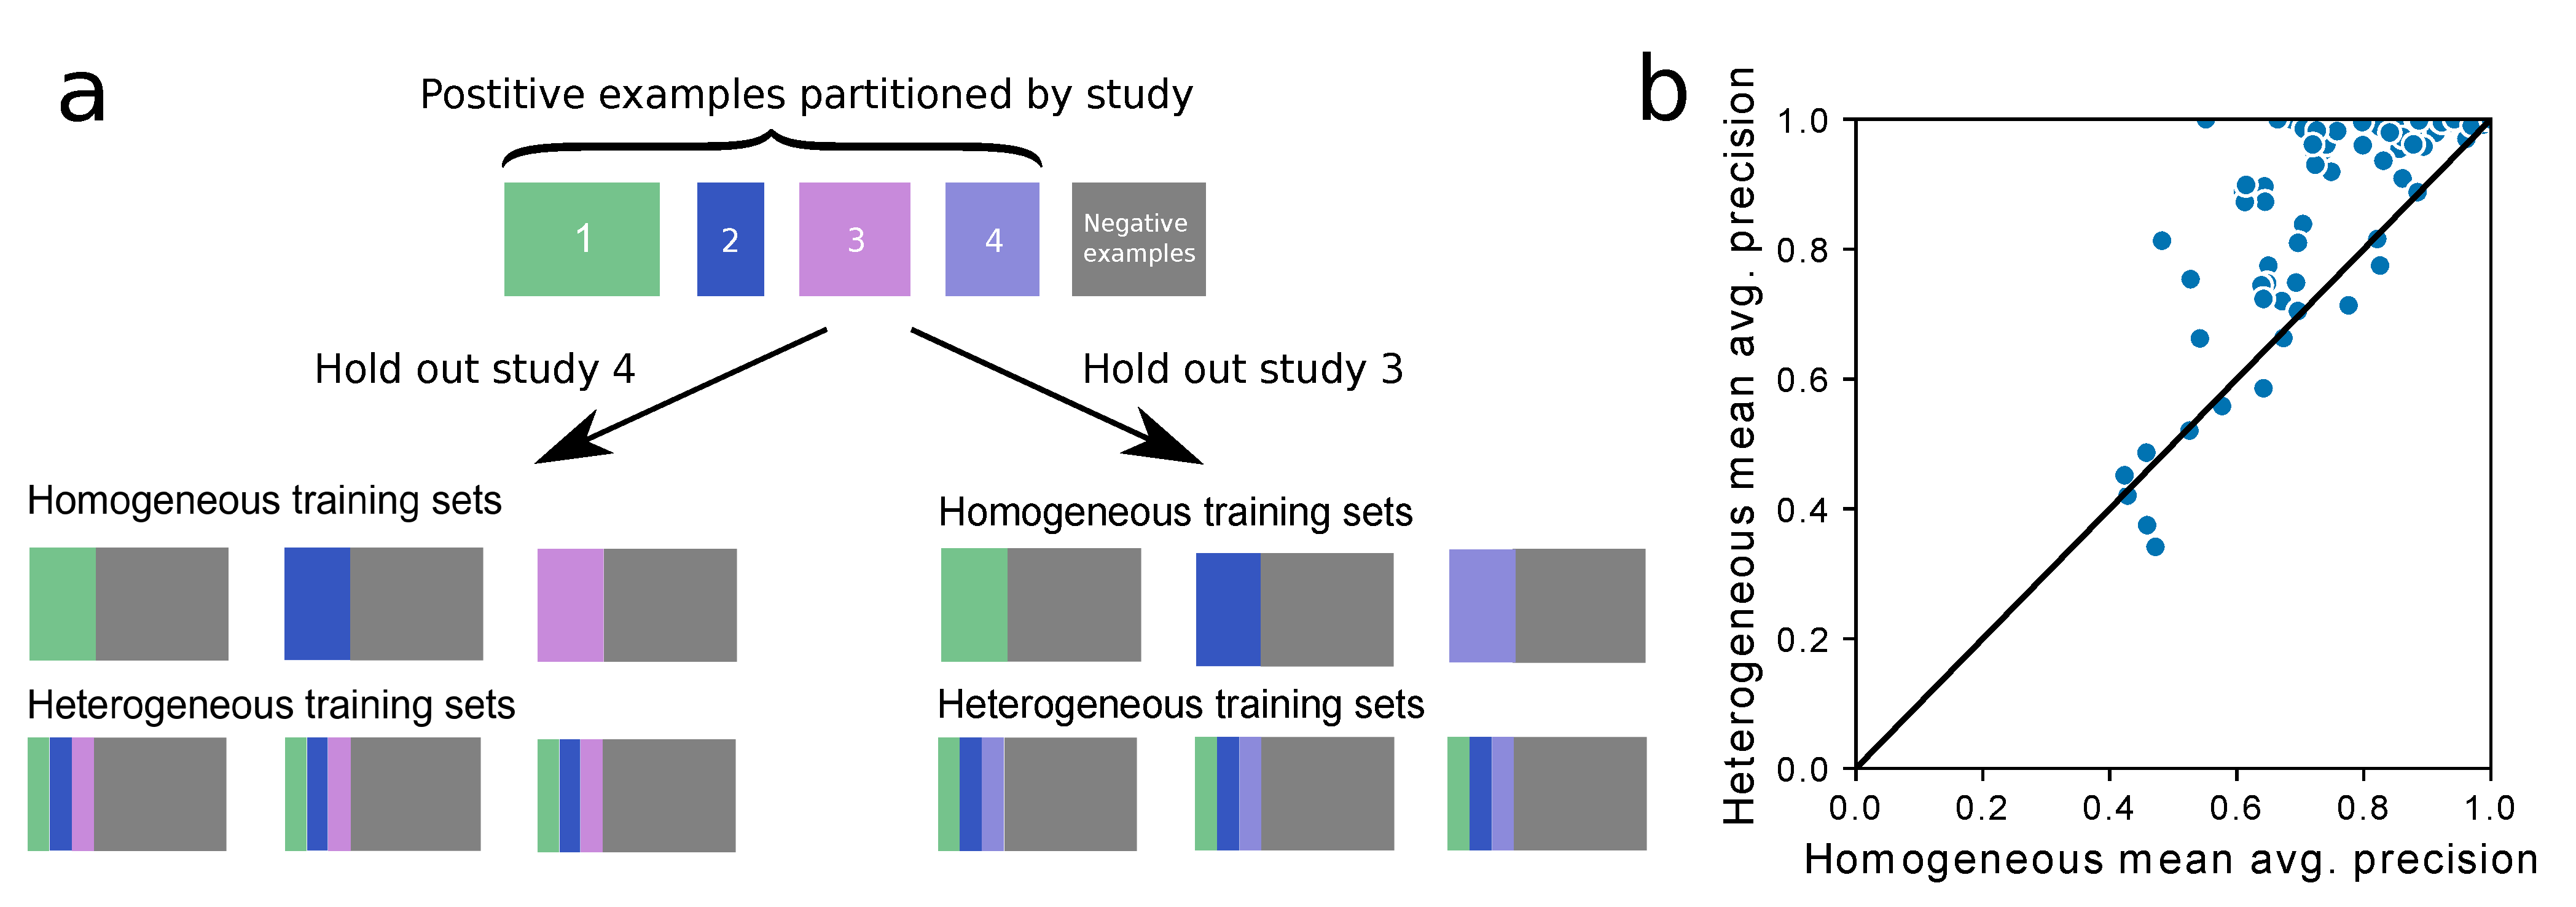
\includegraphics[width=13cm]{figures/homo_vs_hetero_full.pdf}}
  \caption{
     \textbf{Examining the effects of training on heterogeneous data.} (a) A schematic illustrating the experimental setup for our investigation into the effects of training on data from multiple studies versus training on data from a single study.  For a given cell type, we find all studies that contained at least ten samples for that cell type. The numbered colored rectangles illustrate such samples partitioned by their study. We then hold out each study and construct two sets of training sets -- one set of homogeneous training sets and another of heterogeneous training sets.  A classifier is trained on each training set and evaluated on data in the held out study. Above, we illustrate the training sets constructed when holding out studies 3 and 4. Each training set uses an identical set of negative examples and identical sized sets of positive examples (the minimum number of samples in a given study partition). (b) Comparing the mean-average precision across cell types between the homogeneously trained classifiers and the heterogeneously trained classifiers on each held out study.}
      \label{fig:homo_vs_hetero_setup}
      \end{figure}


\subsection*{Evaluation on bulk RNA-seq data}

We evaluated the aforementioned hierarchical classification algorithms using the per-cell type (Fig.~\ref{fig:results_test_bulk}a-b, Fig.~\ref{fig:bulk_pairwise}), per-sample (Fig.~\ref{fig:results_test_bulk}c), and joint (Fig.~\ref{fig:results_test_bulk}d) modes of evaluation.  Overall, we find that IR, TPR, CLR, and independent classifiers performed similarly and better than the baseline BNC and nearest-neighbor algorithms. The similar performance of IR, TPR, and CLR to the independent classifiers demonstrates that reconciling the outputs of the independent predictions with the ontology structure does not degrade performance.  We note that these results are in line with work by Obozinski \textit{et al.} (2008), which demonstrates that IR and CLR outperform BNC on the hierarchical protein function prediction task.

Regarding the per-sample mode evaluation, we note that mean performance on a sample's most-specific cell types was below that of the mean performance when considering all of the sample's cell types (Fig.~\ref{fig:results_test_bulk}c).  We posit three reasons for this: first, it is likely easier for the classifiers to distinguish broad categories of cell types than it is to distinguish fine-grained cell types for which cell-type-specific expression signatures may be more subtle. Second, the amount of training data supporting each cell type strictly decreases down the ontology. Third, we note that a subset of the errors are due to the classifiers providing significant probability to more specific cell types than the most-specific true cell types for a given sample (e.g., a T cell sample predicted to be a CD4+ T cell sample). This may be due to the prevalence of an unlabeled, more-specific cell type in some heterogeneous bulk RNA-seq samples.     

\begin{figure}[h!]
      \centerline{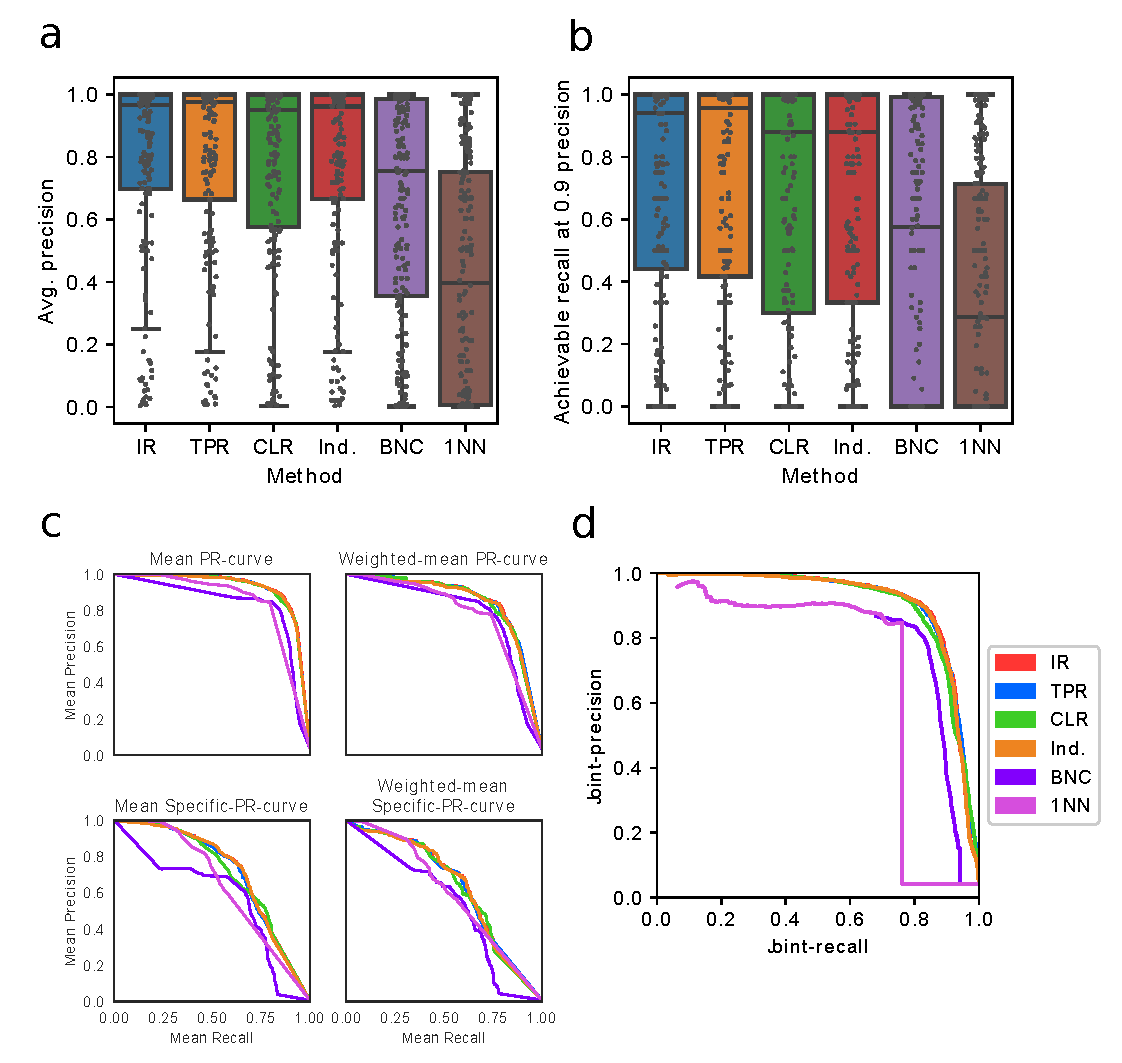
\includegraphics[width=13cm]{figures/bulk_test_set_results.pdf}}
      \caption{\textbf{Bulk test set results.} (a) Comparison between the distributions of average-precision generated by each method across all cell types.  (b) Comparison of the distributions over the highest achievable recalls when precision is fixed at 0.9 across all cell types. (c) Variants of the mean precision-recall curves for comparing the average performance of each method across all samples. (d) The joint-precision recall curves for all methods generated by ranking all sample-cell type output probabilities jointly.}
      \label{fig:results_test_bulk}
      \end{figure}

\begin{figure}[htbp]
    \centerline{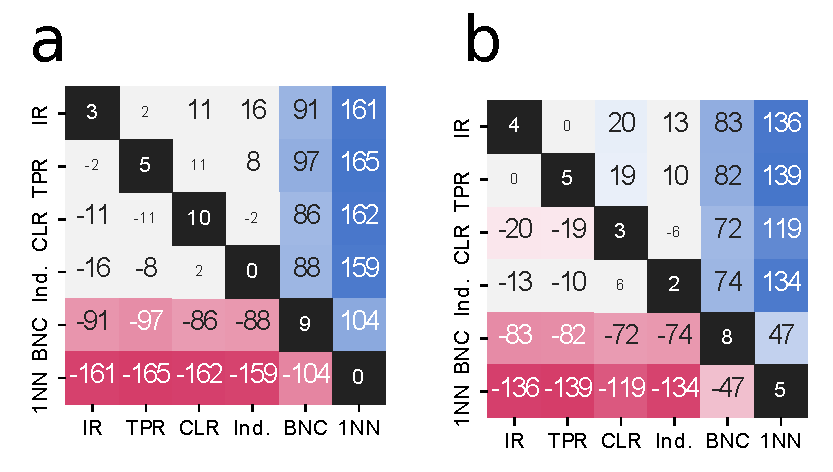
\includegraphics[width=13cm]{figures/bulk_test_pairwise_heatmaps.pdf}}
    \caption{\textbf{Pair-wise comparison of methods on bulk RNA-seq test set.} Heatmaps displaying the pair-wise difference in the number of cell types for which one method beats the other method by more than 0.05 for all pairs of methods using (a) per-cell-type average-precision score and (b) per-cell-type achievable recall at 0.9 precision. For each pair of methods, we also perform a Wilcoxon signed-rank test to assess the whether there exists a significant difference in (a) average precision values and (b) achievable recall at 0.9 precision across the cell types.  We note that this test will be aggressive as the average precision values across cell types are not independent. We bold the entries in the heatmap when p $<$ 0.05.  The diagonal entries present the number of cell types for which the corresponding row's method beat all other methods in (a) average-precision and (b) achievable recall at 0.9 precision by more than 0.05.}
    \label{fig:bulk_pairwise}
      \end{figure}

\subsection*{Evaluation on single-cell RNA-seq data}

We trained the IR, TPR, and CLR algorithms on the entire set of bulk RNA-seq data and evaluated them on the test set consisting of \BulkRestrictedSingleCellExperiments{} single-cell RNA-seq samples whose cell types appear in the bulk RNA-seq training data. We note that many cells were labeled as a broad cell type rather than a specific cell type. For example, in study ERP017126, many cells are described by the data as general pancreatic cells. These samples are likely missing cell type labels because they should, in theory, be labeled with a specific cell type (i.e., lower in the ontology) due to the facts that each sample originates from a single cell and that there are known subtypes of pancreatic cells.  We therefore modified our evaluation metrics to take into account these ambiguous, generally-labeled single-cell samples so as not to penalize the algorithms for predicting cell types more specific than their given labels. We found that these algorithms perform well in all modes of evaluation using these modified metrics (Fig.~\ref{fig:results_test_single}, Fig.~\ref{fig:sc_pairwise}, Fig.~\ref{fig:sc_pr_curves}). 

 \begin{figure}[h!]
       \centerline{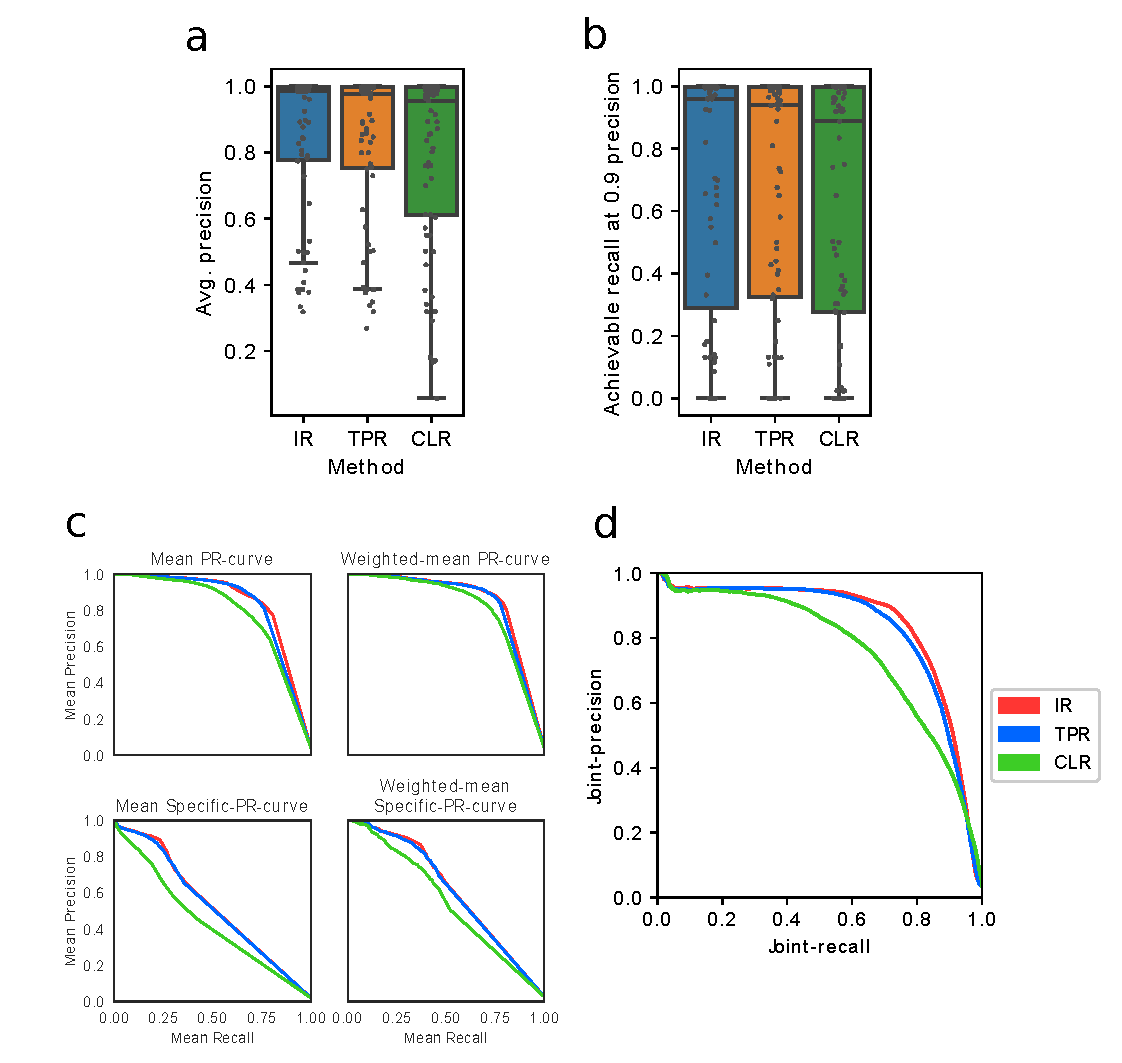
\includegraphics[width=13cm]{figures/single_cell_test_results.pdf}}
       \caption{\textbf{Single-cell test set results.}  (a) Comparison between the distributions of average-precision generated by each method across all cell types.  (b) Comparison of the distributions over the highest achievable recalls when precision is fixed at 0.9 across all cell types. (c) Variants of the mean precision-recall curves for comparing the average performance of each method across all samples. (d) The joint-precision recall curves for all methods generating by ranking all sample-cell type output probabilities jointly.}
      \label{fig:results_test_single}
      \end{figure}

\begin{figure}[htbp]
    \centerline{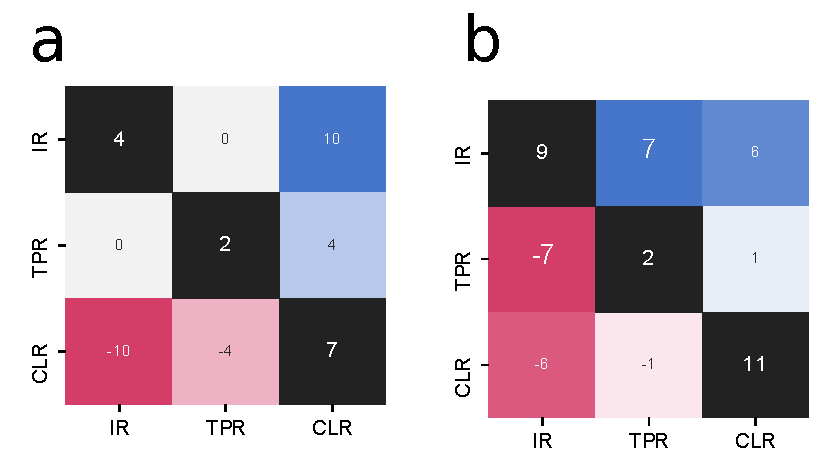
\includegraphics[width=13cm]{figures/sc_pairwise_heatmaps.pdf}}
    \caption{\textbf{Pair-wise comparison of methods on bulk RNA-seq test set.} Heatmaps displaying the pair-wise difference in the number of cell types for which one method beats the other method by more than 0.05 for all pairs of methods using (a) per-cell-type average-precision score and (b) per-cell-type achievable recall at 0.9 precision. For each pair of methods, we also perform a Wilcoxon signed-rank test to assess the whether there exists a significant difference in (a) average precision values and (b) achievable recall at 0.9 precision across the cell types.  We note that this test will be aggressive as the average precision values across cell types are not independent. We bold the entries in the heatmap when p $<$ 0.05.  The diagonal entries present the number of cell types for which the corresponding row's method beat all other methods in (a) average-precision and (b) achievable recall at 0.9 precision by more than 0.05.}
    \label{fig:sc_pairwise}
      \end{figure}

 \clearpage
\begin{sidewaysfigure}%
    \thispagestyle{empty}
    \hspace{-7cm}
    \centering
    {{\includegraphics[width=24cm]{figures/sc_pr_curves_on_graph.pdf} }}%
    \qquad
    {\hspace*{-10cm}{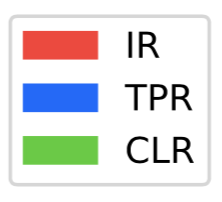
\includegraphics[width=2cm]{figures/sc_legend.png} }}%
    \caption{\textbf{scRNA-seq test set precision-recall curves.} Precision-recall curves for each cell type on the scRNA-seq test dataset. Each node is colored according to which method yielded the highest average precision. The intensity of the color corresponds to the difference between the highest average-precision and the second highest average-precision achieved for that node.}%
    \label{fig:sc_pr_curves}%
\end{sidewaysfigure}
\clearpage

Next, we examined the predictions performed on cells that represented challenging cases for the classifiers. Specifically, we identified two categories of challenging samples: samples that were only  labeled with a broad cell type and samples labeled with a combination of cell types that do not appear in the training data. We examined two studies, SRP067844 and ERP017126, that contained samples that were representative of these challenges and examined their predictions in depth.

When given samples labeled as a general cell type, but not a more specific cell type, the algorithm often predicted a more specific cell type than the labeled cell types.  Study SRP067844 included a set of samples labelled only as embryonic, neural cells, but not as a more specific cell type. In such instances, the algorithm often labeled them as the more specific label, ``neuron", which may be accurate given that this study sought to sequence cells from the developing nervous system (Fig.~\ref{fig:difficult_single_cells}a) (\citealp{Manno2016}). Study ERP017126 contained a set of pancreatic cells that were unlabeled for a specific pancreatic cell type.  Many of these cells were predicted as a specific endocrine cell type such as pancreatic alpha cells (Fig.~\ref{fig:difficult_single_cells}b).

When the methods were provided a query that should be assigned with a combination of labels that it had not seen before during training, its outputs were reasonable. Study SRP067844 consisted of embryonic neural cells. Although the training data contains samples of both embryonic cells and cells of various neural cell types, it does not contain any sample labeled as \textit{both} neural cell \textit{and} embryonic cell. For these samples, we found that the algorithm was often able to label these samples as ``neural cell", but often failed to label them as ``embryonic cell". Furthermore, the algorithm had difficulty labeling these samples with their specific neural cell types such as ``radial glial cell" (Fig.~\ref{fig:difficult_single_cells}c). Similarly, study ERP017126 contained various pancreatic cell types that did not exist in the training data such as pancreatic delta cells and pancreatic ductal cells. We found that the delta cells were often predicted correctly as enteroendocrine cells (Fig.~\ref{fig:difficult_single_cells}d) and were not confused with similar pancreatic endocrine cell types such as alpha cells or beta cells. Similarly, pancreatic ductal cells were often predicted as secretory cells (Fig.~\ref{fig:difficult_single_cells}e). Although the term ``secratory cell" is not an ancestral term of ``pancreatic ductal cell" in the Cell Ontology, these predictions may nonetheless be considered correct predictions given that pancreatic ductal cells are known to secrete biocarbonate (\citealp{Grapin-Botton2005}). 
  
\clearpage
 \begin{sidewaysfigure}
    \thispagestyle{empty}
    %\vspace{-4.5cm}
    \centerline{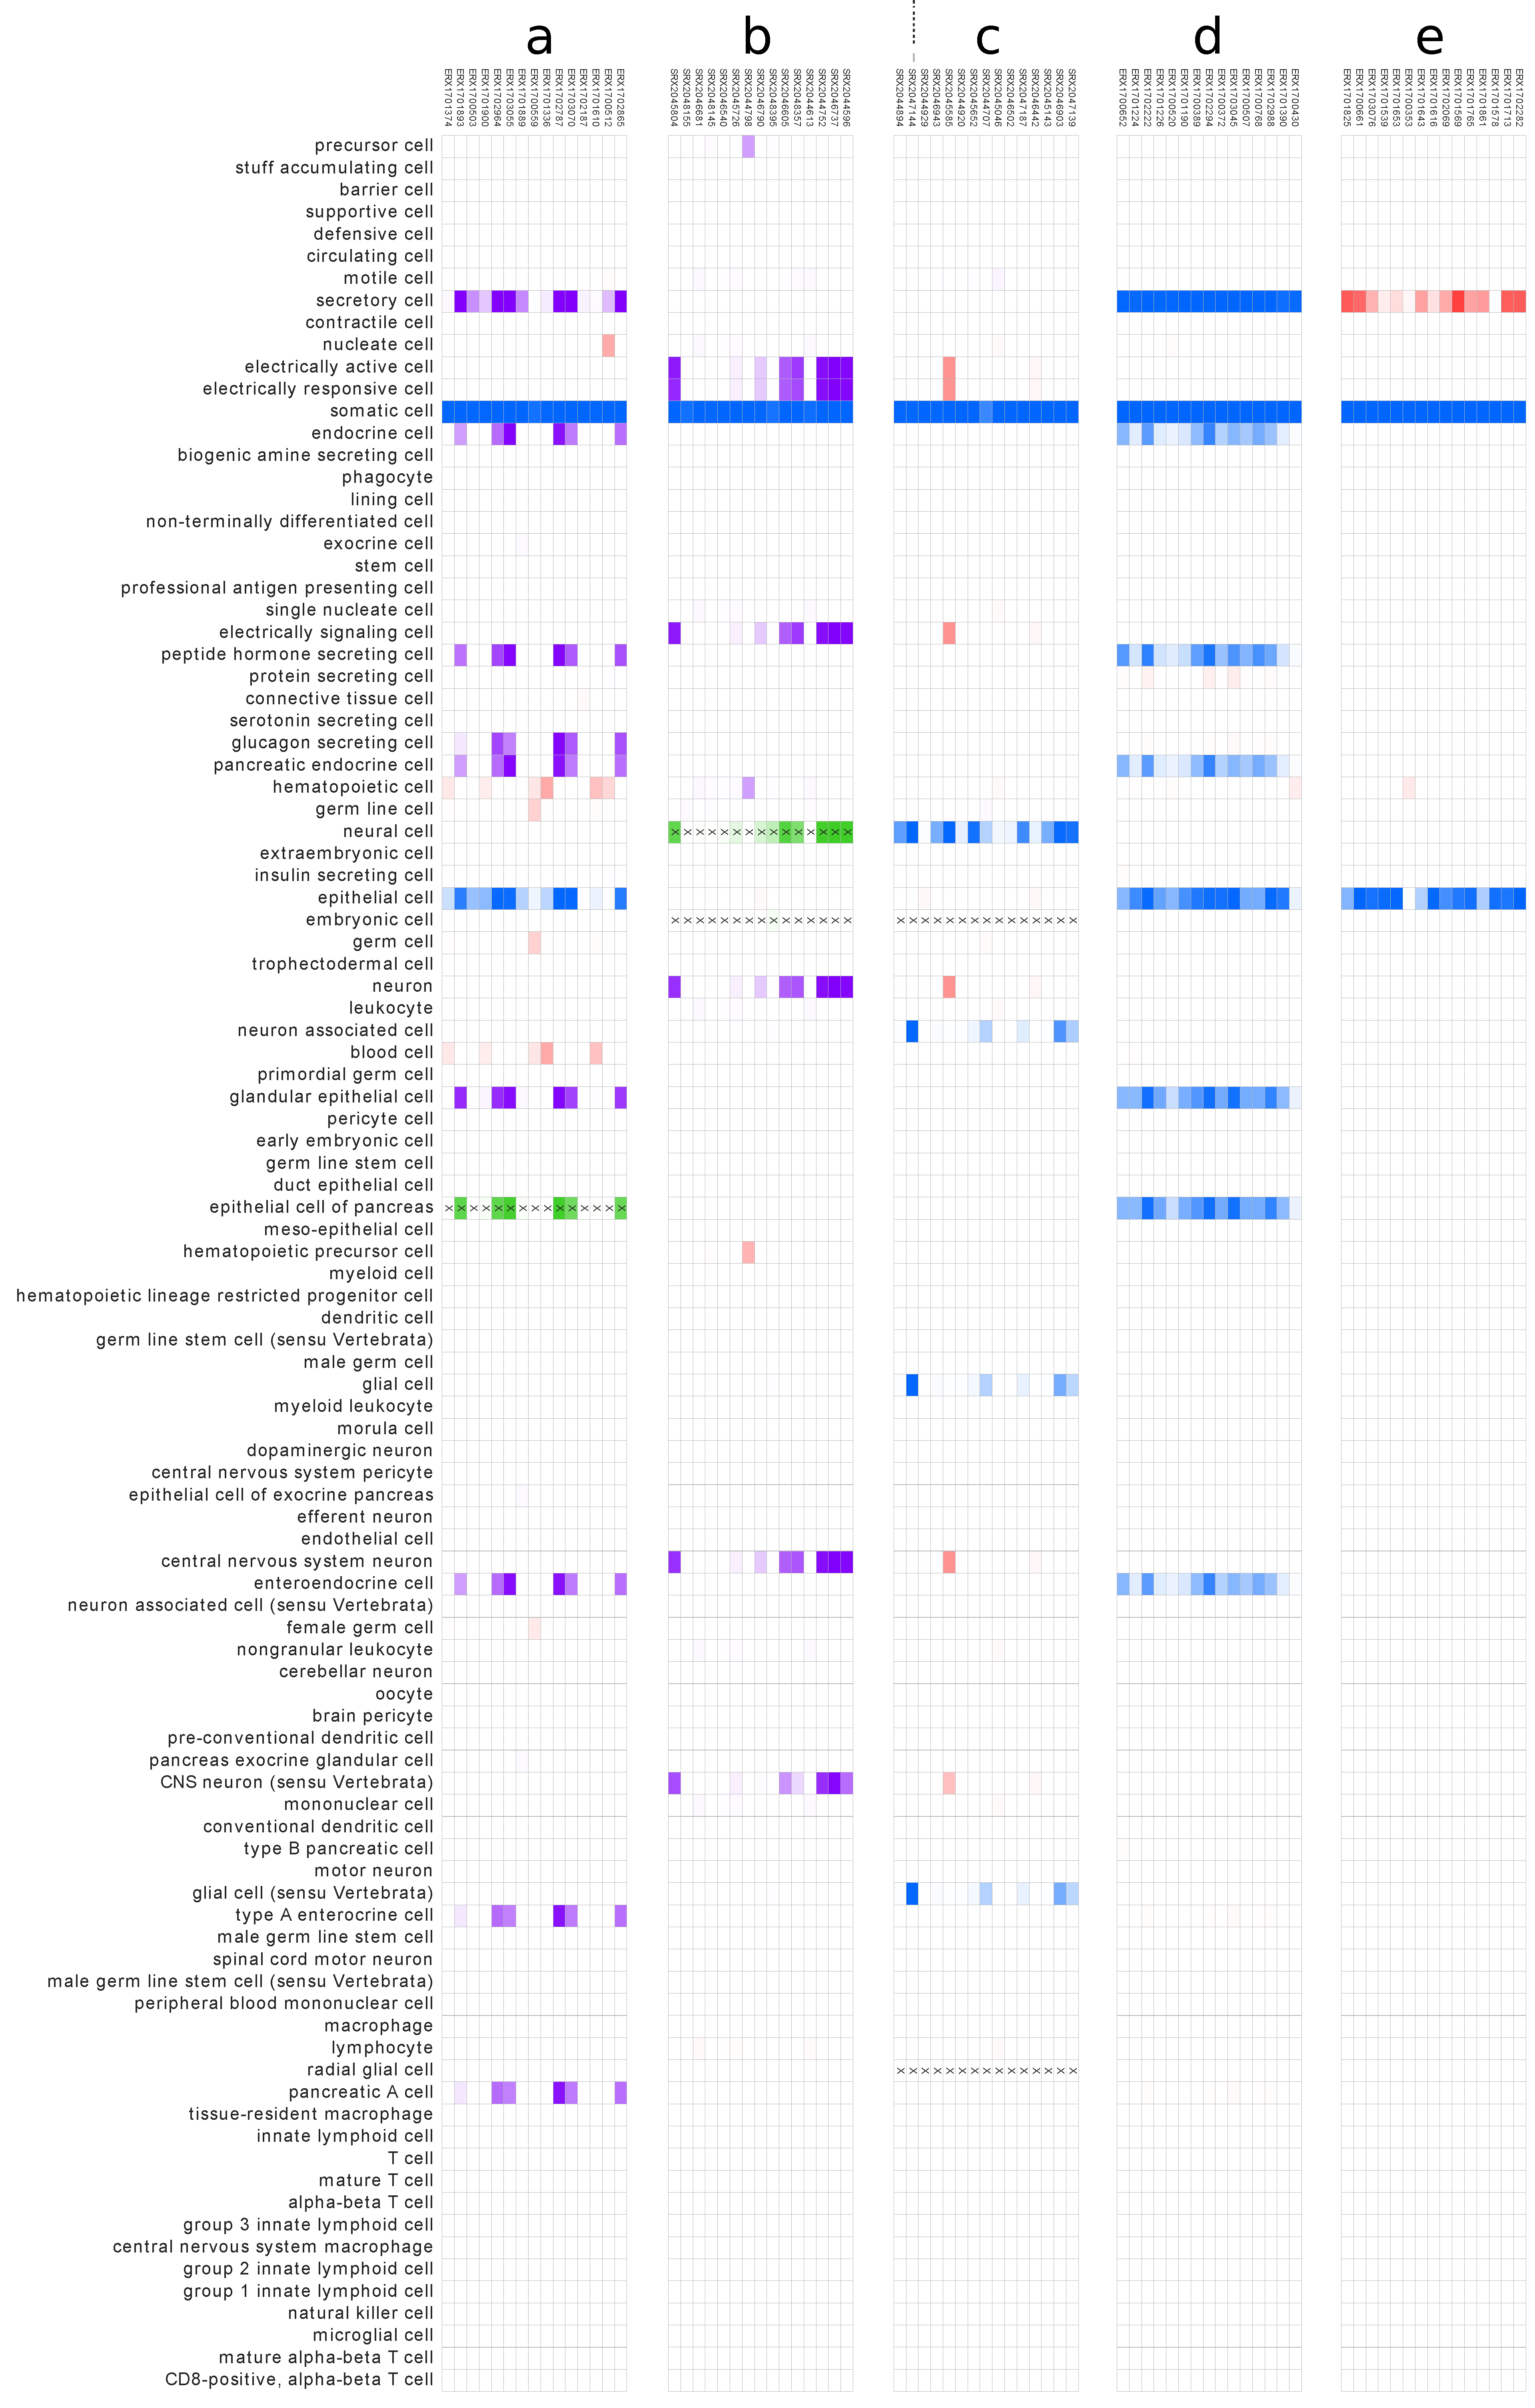
\includegraphics[scale=0.20, angle=-90]
    {figures/all_prediction_matrices_subsamples.pdf}}
   \caption{\textbf{Predictions on challenging single-cell samples.} Randomly sampled output from the IR classifier on difficult-to-classify single-cell samples. Columns correspond to cells and rows correspond to cell types that appeared in the training data. The intensity of each element is proportional to the output probability for the corresponding sample and cell type. Each element is colored according to the relationship between the sample and the cell type. Green denotes a prediction of a most-specific true cell type (annotated with an 'X') for the sample. Blue denotes a prediction of a less-specific, but true cell type. Purple denotes ambiguous predictions that cannot be verified as correct or incorrect (descendents of the sample's true cell types as well as ancestors of those descendents). Red denotes a likely error (a cell type that is neither a true cell type, descendant of a true cell type, nor ancestor of a descendent of a true cell type). We investigated the predictions of samples that are labeled as general cell types, but not more specific cell types from studies ERP017126 (a) and SRP067844 (b). We also investigated predictions on cell types that did not appear in the training data including embryonic radial glial cells (c), delta cells (d), and ductal cells (e).}
    \label{fig:difficult_single_cells}
      \end{sidewaysfigure} 
        
  
\subsection*{Comparison of interpretability between frameworks}

With the exception of the one-nearest neighbor classifier, the methods that we have explored can be subdivided into two categories: those that train a set of one-versus-rest binary classifiers (BNC, IR, TPR) and the CLR framework, which trains a set of ``local" binary classifiers that classify a sample as a given cell type conditioned on the sample belonging to its parent cell types. We explored the question of whether one framework provides an advantage in model interpretability.  To address this question, we analyzed the gene coefficients in each binary classifier's linear model for enrichment of genes involved in known biological processes. We use the number of enriched biological processes as a quantitative measure of model interpretability.  
Specifically, for each learned binary classifier, we rank the genes by their corresponding coefficients in the linear model. We then performed a gene set enrichment analysis with GSEA (\citealp{Subramanian2005}) on these ranked genes using all  ``biological process" gene sets from the Gene Ontology (GO) (\citealp{Ashburner2000}) that were associated with at least \MinGenesInGOSet{} genes. This analysis targeted enrichment at both the top and bottom of the ranked list of genes, which identified biological processes that were either relatively upregulated or downregulated in a given cell type. We then use a false discovery rate q-value cutoff of 0.05 for proclaiming enrichment.  

We found that the models learned in the CLR framework tended to be enriched for more GO terms than the one-versus-rest frameworks (Fig.~\ref{fig:compare_go_enrichment}). We posit that this phenomenon is due to the fact that since the CLR framework involves the training of binary classifiers that seek to distinguish only between a small set of similar cell types, the CLR's classifiers are ``more focused" than the one-versus-rest classifiers, which seek to distinguish each cell type from \textit{all} other cell types.  Thus, the CLR framework may prove more useful for exploring cell type-specific expression patterns and for finding expression patterns that distinguish similar cell types.  The trained model coefficients can be downloaded for further analysis from \DataDownloadURL{}.

 \begin{figure}[h!]
    \centerline{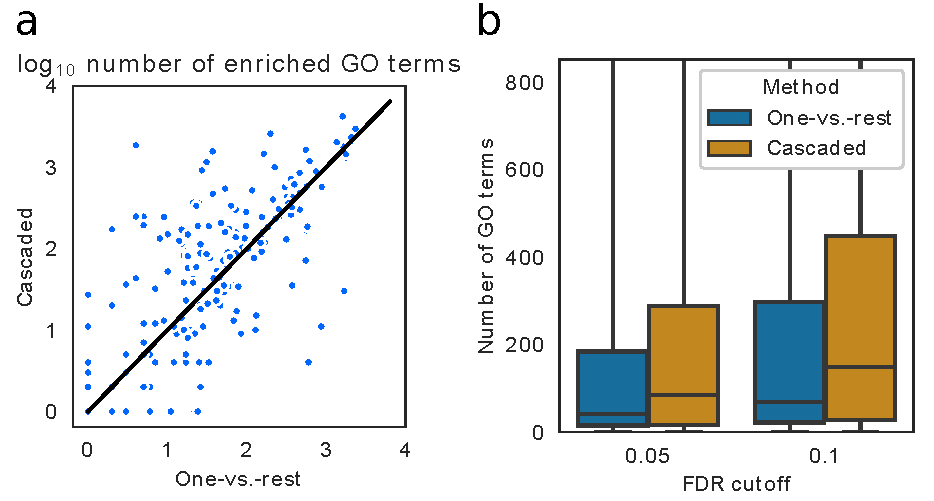
\includegraphics[width=13cm]{figures/GO_enrichment_figure}}
    \caption{\textbf{Gene set enrichment analysis on model parameters.} (a) Comparing the number of GO terms enriched in the ranked list of each binary classifier's coefficients between the cascaded logistic regression and one-vs.-rest frameworks. (b) The distribution of the number of enriched GO terms between these two frameworks using two FDR thresholds for enrichment.}
    \label{fig:compare_go_enrichment}
      \end{figure}



\section{Conclusions}

In this work, we explore the application of hierarchical classification algorithms towards cell type prediction using a novel, well-curated set of human primary cell RNA-seq samples. This dataset may prove useful for future investigations of cell type expression patterns or for use in cell type deconvolution methods (\citealp{Aran2017, Newman2015}). We demonstrate that the trained classifiers perform well across cell types on bulk RNA-seq data and offer a promising approach to cell type annotation in single cell datasets.  

We also found that classification performance is not only dependent on the number of training samples, but also on the diversity of those samples. Specifically, we found that the classifier benefits from training on data from multiple studies. Thus, we argue that the heterogeneity present in the public expression data presents an opportunity to learn robust models. This observation may extend beyond cell type prediction to other phenotype prediction tasks such as expression-based disease prediction.

Furthermore, by using linear models, the trained parameters are easily interpreted as cell type specific signatures across the ontology.  However, we note that since certain cell types undergo similar sorting and preparation procedures (e.g., fluorescence activated cell sorting), it remains unclear to what extent these procedures affect gene expression and thus confound with cell type. We sought to mitigate this effect by using data from a diversity of studies.  We also note that the CLR algorithm may help to further mitigate this effect, since the binary classifiers trained in this framework for each cell type condition on the sample belonging to the parent cell types. Thus, for a given cell type, if the parent cell types were prepared through similar procedures, the learned model parameters for that cell type will better capture biological cell type signatures. 

Finally, we expect the performance of hierarchical classifiers to improve as both more data is collected and as the Cell Ontology is expanded. More data will be collected both as data is continually added to the SRA and as improvements are made to the SRA's metadata thereby allowing retrieval of previously undiscovered primary cell samples.   

\section{Methods}
A schematic diagram of the experiments performed in this chapter is given in Figure~\ref{fig:cell_type_setup}.

\begin{figure}[htbp]
    \centerline{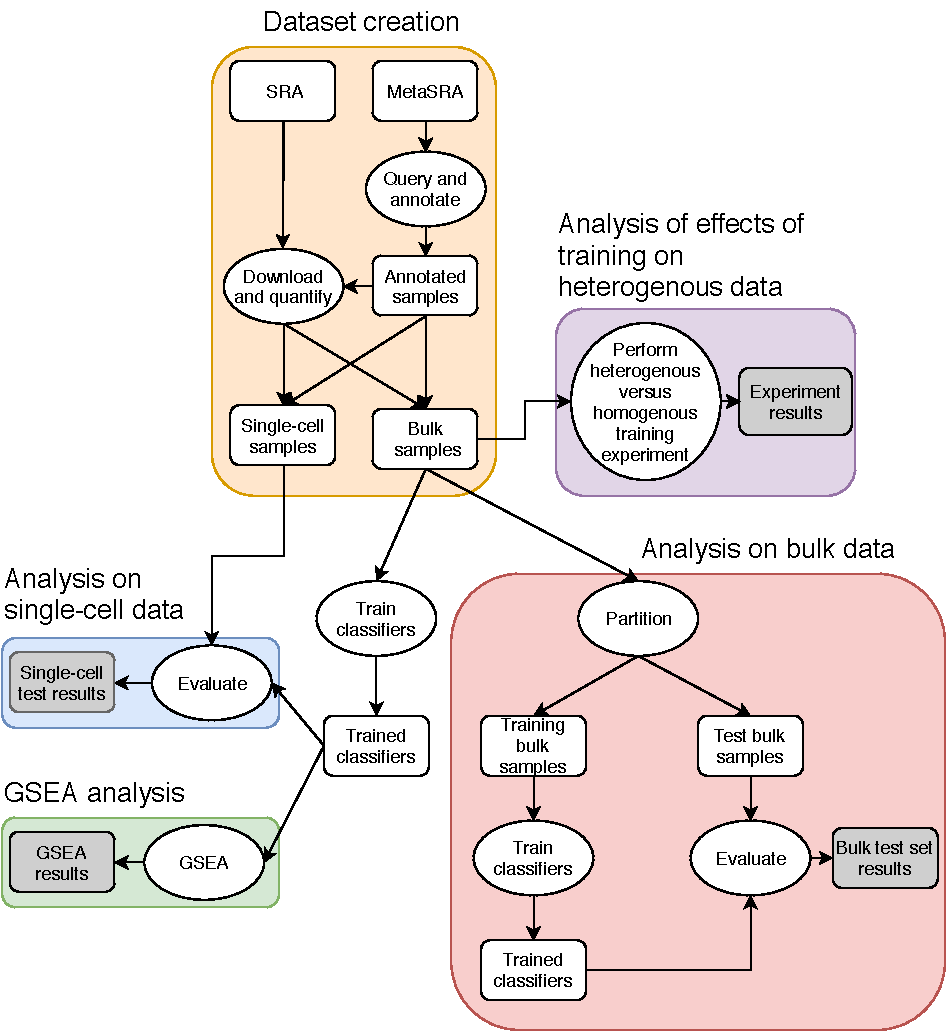
\includegraphics[width=13cm]{figures/cell_type_prediction_setup.pdf}}
    \caption{\textbf{Data flow diagram.} A data flow diagram illustrating data retrieval, annotation, partitioning, training, and analysis involved in this work.}
    \label{fig:cell_type_setup}
      \end{figure}

\subsection*{Data processing}

We quantified the gene expression of all samples with kallisto (v0.43.1) (\citealp{Bray2016}) against the human genome release GRCh38 with GENCODE annotation version 27. We chose kallisto for gene expression quantification in order to prioritize processing speed on this large dataset, figuring that any small loss in accuracy (at the gene level) relative to a less approximate, but slower method would not be significant for the cell type classification task. This produced estimated counts for \RawGenomicFeatures{} isoform-level genomic features. We summed these counts by gene to produce counts for \GeneLevelFeatures{} gene-level features. The curated metadata and associated quantified samples are available to download at \DataDownloadURL{}.


\subsection*{Partitioning bulk RNA-seq data into training and test sets}

When creating a training and test partition of the bulk RNA-seq data, we sought to satisfy a number of criteria that would enable unbiased estimation of performance across cell types:

\begin{enumerate}
    \item No study should be split between the training and test sets. This mitigates the possibility that the algorithm will provide an overly optimistic estimate of the generalization error when run on the test set. 
    \item 80/20 split of the data between the training and test sets.
    \item Maximized overlap of cell types in both the training and test sets to enable training and evaluation on as many cell types as possible.
    \item  For all cell types represented by three or more studies, at least two of those studies should be assigned to the training set. This criteria enables us to perform leave-study-out cross-validation only on the training set, thereby allowing us to evaluate various algorithms on the training set before performing a final analysis on the test set.  
\end{enumerate}
We formulate the data partitioning problem as an optimization problem and attempt to arrive at a ``best" partition that balances the aforementioned four goals.

For this section, we will use the following notation: Let $\mathcal{C}$ be the set of cell types represented in our data. Let $m$ denote the number of studies representing samples in the dataset. Let $S_1, \dots, S_m$ be the sets of cell types in each study.   That is, $S_i \subseteq \mathcal{C}$ where $c \in S_i$ if a sample labeled with cell type $c$ is included in study $i$.  Since we must ensure that the training-test partition is split along study boundaries, we define indicator variables $x_1, \dots, x_m$ that indicates whether each study $i \in [m]$ is included in the training set. Let $\boldsymbol{x} \in \{0, 1\}^m$ be the vector consisting of these indicator variables. 

Using this notation, we can mathematically describe each of the aforementioned goals:
\begin{enumerate}
\item We seek a partition such that some proportion $t$ of studies are in the training set and $1-t$ are in the test set.  We set $t := 0.8$.  We can encode how far we are from achieving this goal using the following function:
$$g_1(\boldsymbol{x}) := \left| \frac{1}{m}||\boldsymbol{x}||_1 - t \right|$$
 \item We seek to maximize the number of cell types represented in both the training and test sets. We encode this goal using the following function: $$g_2(\boldsymbol{x}) := \frac{1}{\mathcal{C}}
\left|\bigcup_{i : x_i = 1} S_i \ \Delta \ \bigcup_{i : x_i = 0} S_i\right|$$
where $\Delta$ is the symmetric difference operation.  
\item For each of those cell types that are represented by at least three studies, we would like to include at least two of those studies in the training set. For a given $\boldsymbol{x}$, let $h(\boldsymbol{x})$ be the fraction of cell types represented by at least three studies that appear at least twice in the training data. Then, our third goal can be described as:
$$g_3(\boldsymbol{x}) := 1 - h(\boldsymbol{x})$$
\end{enumerate}
We then attempt to minimize the following objective function:
$$f(\boldsymbol{x}) := \lambda_1 g_1(\boldsymbol{x})  + \lambda_2 g_2(\boldsymbol{x}) + \lambda_3\ g_3(\boldsymbol{x})$$
Each term in the objective function reflects one of our goals.  The weights $\lambda_1$, $\lambda_2$, $\lambda_3$ set the importance that we place on meeting each goal.  We used a simple hill-climbing procedure to find a partition of the data that minimizes this objective function.

\subsection*{Description of algorithms}

In the following descriptions of the algorithms used in this work, we let $\boldsymbol{x} \in \mathbb{R}^G$ denote a gene expression profile, in units of log-counts per million (log-CPM), where $G$ is the number of considered genes.  Specifically, for gene $i$ in $\boldsymbol{x}$, log-CPM is defined as
$$x_i := \log\left(\left[\frac{c_i}{\sum_{j=1}^G c_j} \times 10^6\right] + 1\right)$$ where $c_i$ is the expected number of reads mapped to the $i$th gene.  We let $n$ denote the number of samples, $m$ denote the number of considered cell types, $y_i \in \{0, 1\}$ denote the cell type assignment for cell type $i \in [m]$, and $\boldsymbol{X}$ denote the training set.

\subsubsection*{Independent binary classifiers}

We used logistic regression with L2-regularization, using scikit-learn (v.0.20.2), for all independent binary classifiers trained in the CLR, IR, and TPR frameworks as well as in the independent classifier baseline method. Our choice of L2 penalty over L1 penalty was motivated by our goal of training interpretable models. Specifically, because the L1 penalty induces sparsity, we were concerned that it would lead to zeroing-out the coefficients of important cell-type-specific genes when such genes correlated highly with other predictive genes. That is, we sought for our models to weight \textit{all} genes according to their predictive ability. 


\subsubsection*{One-nearest neighbor}

Given a query gene expression profile $\boldsymbol{x}$, we return all cell type labels belonging to the training set expression profile
$$\text{arg min}_{\boldsymbol{x}' \in \boldsymbol{X}} \ 1 - \text{Corr}(\boldsymbol{x}, \boldsymbol{x}')$$
where $\text{Corr}(\boldsymbol{x},\boldsymbol{x}')$ is the Pearson correlation of the expression values in $\boldsymbol{x}$ and $\boldsymbol{x}'$.

\subsubsection*{Cascaded logistic regression}

Classification is made in a top-down fashion starting from the root of the ontology downward as proposed by Obozinski \textit{et al.} (2008). This is accomplished by training a logistic regression, binary classifier for each cell type $i \in [m]$ to model the distribution 
$$q_i := p(y_i = 1 \mid \pi_i=1, \boldsymbol{x})$$ 
where $\pi_i \in \{0, 1\}$ indicates whether the sample belongs to all of the parents of $i$ in the ontology. In order to model these distributions, each cell type's negative training examples consist of those samples that are labeled with all parent cell types, but not the target cell type. Given these learned distributions, the probability that $\boldsymbol{x}$ originates from cell type $i$ is computed via  
$$p(y_i = 1 \mid \boldsymbol{x}) = q_i \prod_{j \in A_i} q_j$$ 
where $A_i$ denotes the ancestors of cell type $i$ in the ontology's DAG. 

\subsubsection*{Bayesian Network Correction}

A support vector machine (SVM) binary classifier is trained for each cell type using a linear kernel and a one-versus-rest training strategy. The classifier outputs are then reconciled with the ontology graph using a Bayesian network as proposed by Lee \textit{et al.} (2013).  The true assignments for each cell type, denoted $y_1, \dots, y_m$, are modelled as latent random variables, and the classifier outputs, denoted $f_1(\boldsymbol{x}), \dots, f_m(\boldsymbol{x})$ (signed distances to each decision boundary), are modelled as observed random variables in a Bayesian network.  The final output probability for cell type $i$ is then the marginal probability
$$p(y_i = 1 \mid f_1(\boldsymbol{x}), \dots, f_m(\boldsymbol{x}))$$
Due to the size of the ontology, we perform approximate inference using Gibbs sampling rather than exact inference using the Laurintzen algorithm as was performed by Lee \textit{et al.}.

\begin{figure}[htbp]
    \centerline{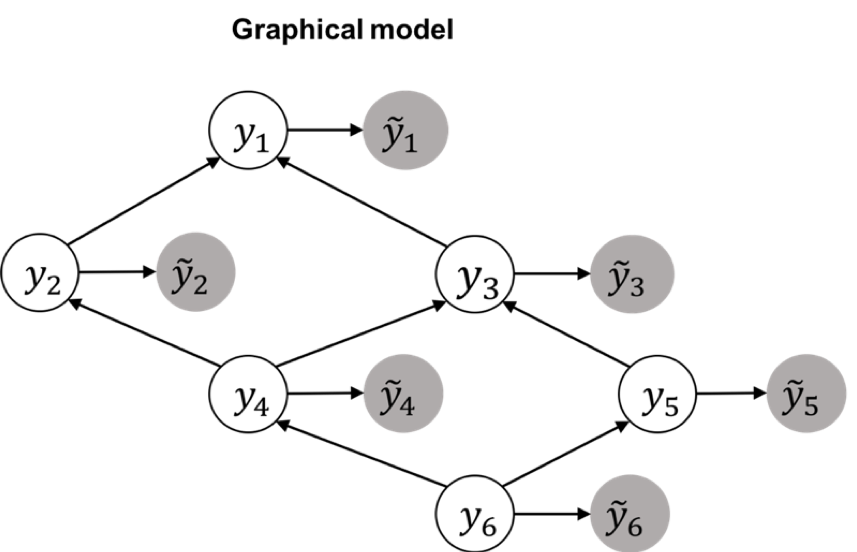
\includegraphics[width=8cm]{figures/BNC_graph.png}}
    \caption{\textbf{Bayesian Network Correction.} An example Bayesian network used in the BNC approach.  Here, $\tilde{y}_i := f_i(\bold{x})$ is the random variable representing the SVM score (i.e. signed distance of the hyperplane) of a feature vector $\bold{x}$ according to the trained SVM classifier for cell type $i$.}
    \label{fig:cell_type_setup}
      \end{figure}

\subsubsection*{Isotonic regression correction}

We train a binary classifier for each cell type $i \in [m]$ to model $p(y_i \mid \boldsymbol{x})$ using logistic regression and a one-versus-rest training strategy.  As proposed by Obozinski \textit{et al.} (2008), these probabilities are then reconciled with the ontology graph using isotonic regression. Specifically, we output the set of probabilities 
$$p_1, \dots, p_m := \text{arg min}_{p'_1, \dots, p'_m} \sum_{i=1}^m (p'_i - \hat{p_i})^2$$
subject to 
$$\forall i \in [m], \forall j \in \text{Par}(i), \ p_i < p_j$$
where $\forall i \in [m], \hat{p}_i := p(y_i=1 \mid \boldsymbol{x})$ as output by each classifier and $\text{Par}(i)$ is the set of parent cell types for cell type $i$. 

\subsubsection*{True Path Rule}

We train a binary classifier for each cell type $i \in [m]$ to model $p(y_i \mid \boldsymbol{x})$ using logistic regression and a one-versus-rest training strategy.  As proposed by Notaro \textit{et al.} (2017), this method involves two passes across the ontology: on a bottom-up pass, each cell type's output probability is averaged with the outputs of all child cell types classifiers for which the classifier makes a positive prediction according to a predefined threshold.  More specifically, each cell type $i$'s output probability is set to
$$p_i := \frac{1}{|C_i|+1}\left(\hat{p}_i + \sum_{j \in C_i} \hat{p}_j\right)$$
where $\hat{p}_i := p(y_i=1 \mid \boldsymbol{x})$ according to the classifier and 
$$C_i := \{j \in \text{Children}(i) \ : \ \hat{p}_i > t \}$$ 
is the set of children of cell type $i$ for which the classifier output a positive prediction according to a predefined threshold $t$. We used a threshold of $t = 0.5$.  This bottom-up pass allows sharing of information across the classifiers. In the top-down pass of the ontology, the output probabilities are set to ensure consistency with the ontology.

\subsection*{Per-sample evaluation metrics}

In the per-sample mode of evaluation, we analyze the average performance over each sample. For a given sample, let $T$ be the full set of a true cell type labels and $P$ be the set of predicted labels. The per-sample precision and recall are then defined as
$$
   \text{Precision} := \left\{
     \begin{array}{lr}
       \frac{|T \cap P|}{|P|} & : |P| > 0  \\
       1 & : |P| = 0
     \end{array}
   \right.
$$
$$\text{Recall} := \left\{
     \begin{array}{lr}
       \frac{|T \cap P|}{|T|} & : |T| > 0  \\
       1 & : |T| = 0
     \end{array}
   \right.$$
respectively.  We further define a version of precision and recall, termed \textit{specific-precision} and \textit{specific-recall}, that seek to summarize how well the classifier is retrieving the most granular cell types that describe the sample. Given a cell type label $c$ from the ontology, let $Ch(c)$ be the children of $c$ in the ontology DAG. We then define the most-specific set of true labels and most-specific set of predicted labels as
$$T' := \{c \in T : |Ch(c) \cap T| = 0 \}$$
$$P' := \{c \in P : |Ch(c) \cap P| = 0 \}$$
respectively. Specific precision and recall are then defined as
$$\text{Specific-Precision} := \left\{
     \begin{array}{lr}
       \frac{|T \cap P'|}{|P'|} & : |P'| > 0  \\
       1 & : |P'| = 0
     \end{array}
     \right.$$
$$\text{Specific-Recall} := \left\{
     \begin{array}{lr}
       \frac{|T' \cap P|}{|T'|} & : |T'| > 0  \\
       1 & : |T'| = 0
     \end{array}
     \right.$$
respectively. Given these per-sample measures of precision and recall, we then compute mean precision (MP), mean recall (MR), mean specific-precision (MSP), and mean specific recall (MSR) across all samples. 

Finally, as was noted previously, since samples from the same study perform similarly, these metrics will be most effected by these large studies. To counteract this effect we also define a set of average metrics that use a weighted mean so that each study contributes equally. These metrics, which we call weighted-mean precision (WMP), weighted-mean recall (WMR), weighted-mean specific-precision (WMSP), and weighted-mean specific-recall (WMSR) are defined as
$$WMP := \frac{1}{s}\sum_{i=1}^n \frac{1}{|S_i|}\text{Precision}_i$$
$$WMR := \frac{1}{s}\sum_{i=1}^n \frac{1}{|S_i|}\text{Recall}_i$$
$$WMSP := \frac{1}{s}\sum_{i=1}^n \frac{1}{|S_i|}\text{Specific-Precision}_i$$
$$WMSR := \frac{1}{s}\sum_{i=1}^n \frac{1}{|S_i|}\text{Specific-Recall}_i$$
where $n$ is the total number of samples, $s$ is the total number of studies, and $S_i$ is the set of samples in the study that includes sample $i$. Finally, by varying the prediction threshold, we can compute curves for all of these metrics. Specifically, we compute mean PR-curves, mean specific-PR-curves, weighted-mean PR-curves, and weighted-mean specific-PR-curves.

\subsection{Modified single-cell evaluation metrics}

When evaluating performance of the classifiers on the single-cell test dataset, we modified the evaluation metrics to take into account samples that were labelled with a general cell type, but not a specific cell type. The ground-truth for these more-specific cell types are ambiguous since these samples should, in theory, be labelled with a specific cell type (i.e., a cell type that is low in the ontology DAG) due to the fact that they originate from single cells.  This stands in contrast to bulk RNA-seq samples that may constitute a population of specific cell types for which it would be apt to label such samples with the less specific cell type that covers all of the cell types in the population (e.g. labelling a bulk RNA-seq sample as ``T cell" when it constitutes a heterogeneous population of T cell subtypes).  For many of these ambiguous single-cell samples, we found that the classifier would output a high probability for a more specific cell type than that with which it was labelled. Such predictions by the classifier cannot be verified and therefore we argue that they should neither be rewarded nor penalized in our evaluation metrics. Therefore we modified as metrics as described in the sections below.

\subsubsection{Per-cell type mode of evaluation}

When constructing the precision-recall curves for a given cell type, we exclude those samples that are labelled most-specifically as an ancestor of the cell type. For example, we would exclude from the ``CD8-positive alpha-beta T cell" precision-recall curve those samples that are most-specifically labelled as ``T cell". 

\subsubsection{Per-sample mode of evaluation}

To modify the specific-precision and specific-recall metrics, we take into account those cell types that are more specific than the true cell type label and those cell types that are ancestors of these more-specific labels. For a given sample, let $T$ be the set of true cell type labels and let $P$ be the set of predicted cell type labels. Furthermore, we the define the most specific true cell type labels and most specific predicted labels as 
$$T' := \{x \in T : |Ch(x) \cap T| = 0 \}$$
$$P' := \{x \in P : |Ch(x) \cap P| = 0 \}$$
respectively where $Ch(x)$ is the set of children of cell type $x$ in the ontology.  For a given cell type $x$, let $A(x)$ be the ancestors of $x$ and let $D(x)$ be the descendents of $x$. Then, let $M$ be the descendents of the most specific true cell types. That is,
$$M := \bigcup_{x \in T'} D(x)$$
Since the ontology is a DAG, it holds that $M \cap T = \emptyset$.
We can now define all of the ambiguous cell types as
$$R := M \cup \left(\bigcup_{x \in M} (A(x) \setminus T)\right)$$
Now, we can modify the most-specific predicted labels to be the set of most-specific predicted labels \textit{only} among those cell types that were predicted \textit{and} that are not ambiguous. That is, we define the modified most-specific predicted labels to be
$$P^* := \{x \in (P \setminus R) : |Ch(x) \cap (P \setminus R)| = 0 \}$$
Per-sample precision and recall are then modified to be defined as
$$\text{Precision} := \left\{
     \begin{array}{lr}
       \frac{|T \cap (P \setminus R)|}{|P \setminus R|} & : |P \setminus R| > 0  \\
       1 & : |P^*| = 0
     \end{array}
     \right.$$
$$\text{Recall} := \left\{
     \begin{array}{lr}
       \frac{|T \cap (P \setminus R)|}{|T|} & : |T| > 0  \\
       1 & : |T| = 0
     \end{array}
     \right.$$
respectively.  Specific-precision and specific-recall are then modified to be defined as
$$\text{Specific-Precision} := \left\{
     \begin{array}{lr}
       \frac{|T \cap P^*|}{|P^*|} & : |P^*| > 0  \\
       1 & : |P^*| = 0
     \end{array}
     \right.$$
$$\text{Specific-Recall} := \left\{
     \begin{array}{lr}
       \frac{|T' \cap (P \setminus R)|}{|T'|} & : |T'| > 0  \\
       1 & : |T'| = 0
     \end{array}
     \right.$$
respectively. 




      
         
 

      
       
       
     



% Sentence fragments

% This stands in contrast to bulk RNA-seq data for which it may be suitable to label the samples with less specific cell types when the samples consist of heterogeneous cell types. 

%Over the course of this project, we flagged a number of errors in the Cell Ontology and reported these issues to the Cell Ontology curators.  

\chapter{Cell type classification of sparse single-cell RNA-seq data} \label{chap:3}

\section{Background}

Recent advances in scRNA-seq are enabling higher numbers of cells to be sequenced than ever before. Specifically, droplet-based scRNA-seq protocols are now enabling the sequencing of tens of thousands of cells at a time, thereby enabling the study of cell populations at unprecedented scales and levels of granularity (\citealp{TabulaMuris2018, Zheng2017, Macosko2015}).  Unfortunately, the ability to sequence high volumes of cells comes at the cost of capturing fewer reads per cell, leading to fewer measured genes per cell (Fig.~\ref{fig:sparsity}).  This data sparsity introduces challenges to cell type classification because there is less data to inform each cell's cell type.  

 \begin{figure}[h!]
      \centerline{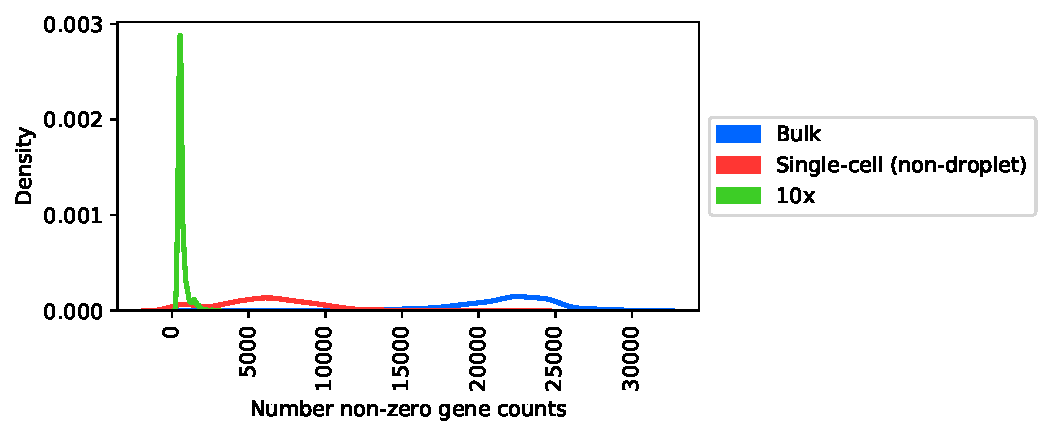
\includegraphics[width=13cm]{figures/num_genes_expressed_distribution.pdf}}
      \caption{\textbf{Sparsity of single-cell assays.} Comparing the sparsity between the bulk RNA-seq dataset, the non-droplet-based scRNA-seq dataset from Chapter~\ref{chap:2}, and 5,000 random cells from the \cite{Zhang2018} 10x scRNA-seq dataset described in Section~\ref{sec:sparse_data}.}
      \label{fig:sparsity}
      \end{figure} 

As these scRNA-seq datasets grow ever larger, rapid cell type classifiers will become more necessary.  This is especially true if this technology is to ever be deployed in a clinical setting where time and computational resources are limited.  The vision is that scRNA-seq will enable new diagnostic tests that entail measuring the transcriptome of specific cell populations (\citealp{Haque2017}).  Due to the limit on computational resources in the clinic, such applications may require phenotyping of individual cells in a streaming fashion where phenotyping is performed on one cell at a time independently from the rest of the cells.  As in Chapter~\ref{chap:2}, we focus on the cell type classification task; however, the methodologies pursued in this chapter may carryover to other single-cell phenotyping tasks. 

The most common techniques for classifying cell type using bulk RNA-seq datasets take a reference-based (i.e. nearest-neighbors-based) classification approach by matching each cell to the most similar bulk RNA-seq expression profile in the reference set (i.e. training set).  Two such methods that take this approach are scMatch (\citealp{Hou2019}) and singleR (\citealp{Aran2019}).  Unfortunately, reference-based classification is computationally expensive with large memory requirements for storing the reference data.  

Very recent work has proposed using neural networks to perform cell type classification on human data (\citealp{Xie2019, Ma2019}). Such an approach may also enable rapid cell type classification as these models do not require extensive computation at test-tme. We note, however, that these methods train on scRNA-seq data, rather than bulk. We also note that neural networks do not easily enable taking into account the hierarchy of cell types, whereas the methods developed in this chapter simply extend binary cell type classifiers and therefore can be easily inserted in to the ensemble-based hierarchical classification frameworks discussed in Chapter~\ref{chap:2}.  

The models developed in Chapter~\ref{chap:2} promise an avenue for efficient and accurate cell type classification. Unfortunately, the models developed in Chapter~\ref{chap:2} were trained on dense, bulk RNA-seq data and therefore, out of the box, they may not be optimal for use on sparse scRNA-seq data.  This chapter addresses this issue by exploring methods for adapting these bulk-trained classifiers for use on sparse scRNA-seq data. To this end, we explored two general strategies for transforming the test data, making it more dense so that it better resembles the training data.  

To this end, we explored two general strategies for adapting the bulk-trained classifiers to sparse data: in the first strategy, we transform the bulk RNA-seq test data, making it more sparse, so that its sparsity matches that of the test data. In the second strategy, we transform the test data, making it more dense so that it better resembles the training data.  

%First, these models have relatively small storage requirements as they need only store the per-gene coefficients for each cell type ($L \times G$ coefficients where $L$ is the number of cell type labels and $G$ is the number of genes), rather than the full reference dataset ($N \times G$ values where $N$ is the number of samples in the reference set). Second, these models allow for fast prediction time as each cell type is associated with a linear model.  Therefore running a query dataset through these models requires a single matrix multiplication step followed by the hierarchical correction step (e.g. isotonic regression).  


Next, we explore the use of gene expression imputation algorithms. Gene expression imputation on scRNA-seq is the task of imputing counts for genes. Emerging approaches for gene expression imputation entail pooling data across cells in the query dataset (\citealp{Dijk2018, Huang2018, Li2018}).  Because these approaches pool data across the query dataset, they require computing on the entire dataset at once and therefore are not apt for a setting in which phenotyping must either be parallelized across cells or in which phenotyping must be performed in a streaming fashion. To address this shortcoming, we develop a novel probabilistic model of the sparse scRNA-seq data-generating process, which implicitly performs gene expression imputation and allows for most computation to occur on the training set, thereby enabling rapid cell type classification in a streaming fashion. 
 
\section{Data}\label{sec:sparse_data}

For the experiments used in this chapter, we utilized both data from Chapter~\ref{chap:2} as well as 10x scRNA-seq data from  \cite{Zhang2018}. We used the bulk RNA-seq data from Chapter~\ref{chap:2} to simulate scRNA-seq data. Specifically, for a given number of total reads $n$ (i.e. level of sparsity), for each sample, we sampled a sparse expression profile according to a multinomial distribution:
 $$\bold{x}_{\text{sparse}} \sim \text{Mult}(n, p_1, \dots, p_G)$$
 where $G$ is the total number of genes and $p_i$ is the fraction of reads assigned to gene $i$.  We created four sparsified versions of the dataset corresponding to four values for $n$: $10^5$, $10^4$, $10^3$, and 100 reads. 
 
 As a test set, we used Chromium 10x scRNA-seq data from \cite{Zhang2018}. Specifically, we used ten peripheral blood mononuclear cell (PBMC) datasets, where each consists of a purified, immune cell type\\(\texttt{https://support.10xgenomics.com/single-cell-gene-expression/datasets}). This dataset is summarized in Table~\ref{tab:10x_pbmc}.  We note that this 10x dataset provides counts for \NumTenXGenes{} genes rather than \GeneLevelFeatures{} genes used in the dataset from Chapter~\ref{chap:2}.  The intersection of these two gene sets was \NumTenXIntersection{} total genes.  We therefore only used these  \NumTenXIntersection{} so that we could train classifiers on our dataset and apply them directly to this 10x data.
 
 \begin{table}[h!]
    \begin{center}
    \begin{tabular}{ |l|c| } 
    \hline
    \textbf{Cell type} & \textbf{No. of cells} \\ \hline
    CD8+/CD45RA+ Naive Cytotoxic T Cells & 11,953  \\
    CD4+ Helper T Cells & 11,213 \\
    CD4+/CD45RA+/CD25- Naive T cells & 10,479  \\
    CD4+/CD25+ Regulatory T Cells & 10,263  \\
    CD4+/CD45RO+ Memory T Cells & 10,224 \\
    CD8+ Cytotoxic T cells & 10,209  \\
    CD19+ B Cells & 10,085  \\
    CD34+ Cells & 9,232  \\
    CD56+ Natural Killer Cells & 8,385 \\    
    CD14+ Monocytes & 2,612 \\
     \hline
    \end{tabular}
    \end{center}
    \caption{\textbf{10x Dataset Summary.} A summary of the ten PBMC FAC-sorted cell types from \cite{Zhang2018}.}
    \label{tab:10x_pbmc}
    \end{table}


 
\section{Results and Discussion}

\subsection{Performance degradation on sparse data}\label{sec:sparse_test}
 
 We first performed an experiment to assess how well the trained classifiers from Chapter~\ref{chap:2} perform on sparse RNA-seq data out-of-the-box.  In this experiment, we applied the independent one-versus-rest classifiers trained on the bulk RNA-seq training set to each of the sparse versions of the test set described in Section~\ref{sec:sparse_data}.  As expected, we found a strong decrease in performance as sparsity increased (Fig.~\ref{fig:results_test_bulk_downsample}).  

 \begin{figure}[h!]
      \centerline{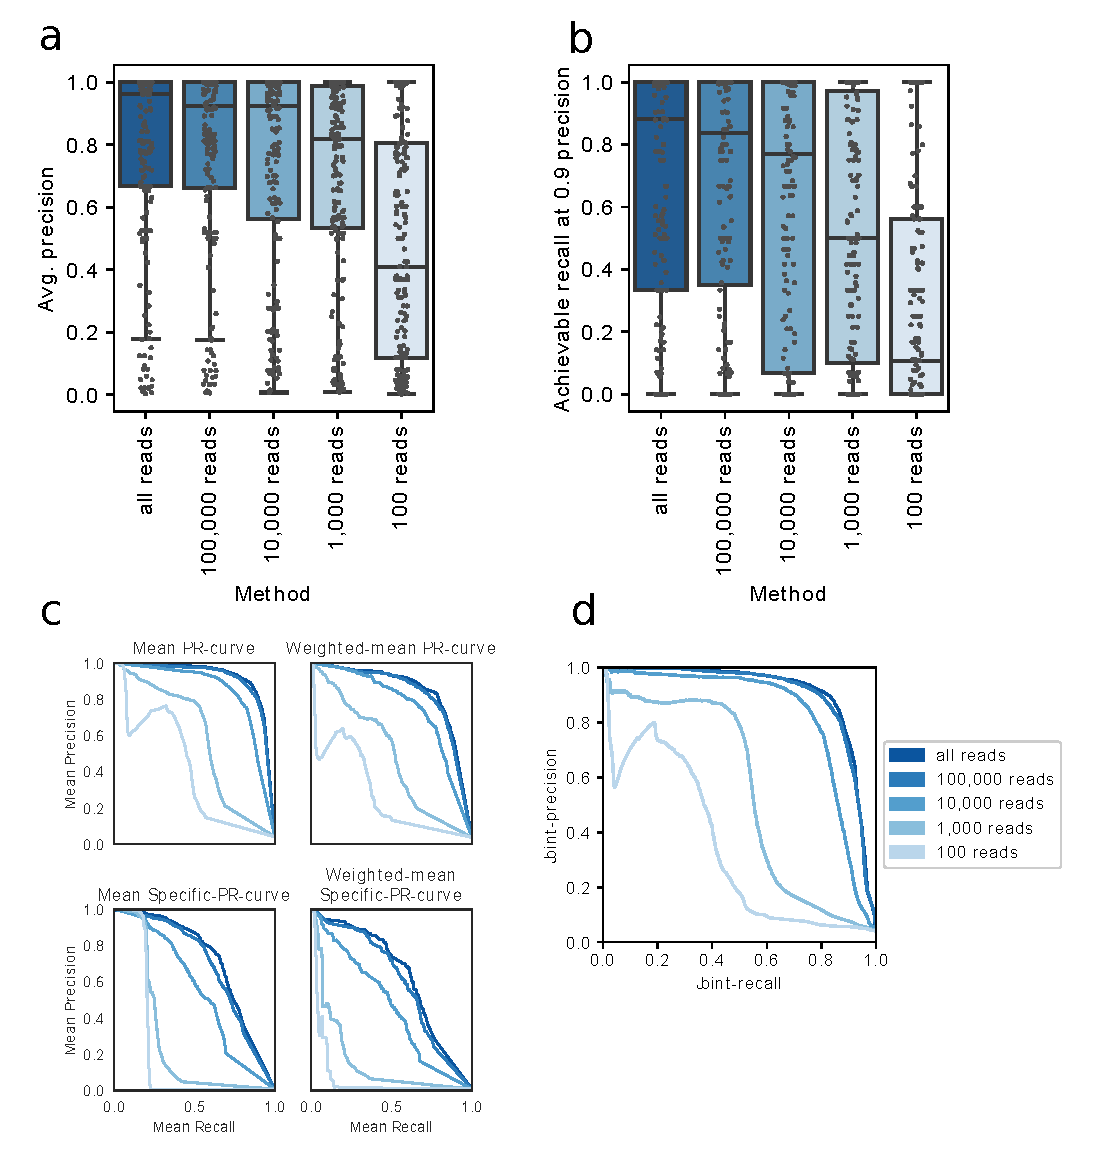
\includegraphics[width=13cm]{figures/bulk_test_set_downsampled_results.pdf}}
      \caption{\textbf{Results on sparse test set.} (a) Comparison between the distributions of average-precision generated by each method across all cell types.  (b) Comparison of the distributions over the highest achievable recalls when precision is fixed at 0.9 across all cell types. (c) Variants of the mean precision-recall curves for comparing the average performance of each method across all samples. (d) The joint-precision recall curves for all methods generated by ranking all sample-cell type output probabilities jointly.}
      \label{fig:results_test_bulk_downsample}
      \end{figure}

\subsection{Training on sparsified bulk RNA-seq data}\label{sec:sparse_test}

We explored an approach in which we trained the classifiers on sparsified bulk RNA-seq data in order to test whether matching the sparseness of the training data to the test data would improve performance. We first  compared the performance of the classifier trained and tested at each level of sparsity to that trained on the full, dense data (Fig.~\ref{fig:results_train_and_test_bulk_downsample}). As expected, we see that training on data that matches the sparsity of the test data improved performance at all read-depths across all modes of evaluation.


%We found that at higher read-depths, training on sparse data tended to hurt performance. Only at very low read-depths did we see a gain in performance when training on data whose sparsity matched the sparsity of the test data.  Interestingly, in the joint evaluation, we found that lower levels of sparsity yielded much poorer performance. Notably, the classifiers that were trained and tested on data sampled down to $10^5$ reads produced the poorest joint PR-curve (Fig.~\ref{fig:results_train_and_test_bulk_downsample}c), even worse than the classifiers trained and tested on data sampled down to 100 reads.  Examining the errors by these classifiers revealed that the independent cell type classifiers were poorly calibrated as indicated by the germ cell classifiers incorrectly producing very high probabilities for most of the test samples (thus, causing the highly ranked predictions to be incorrect when computing the joint PR-curve).  	

 \begin{figure}[h!]
      \centerline{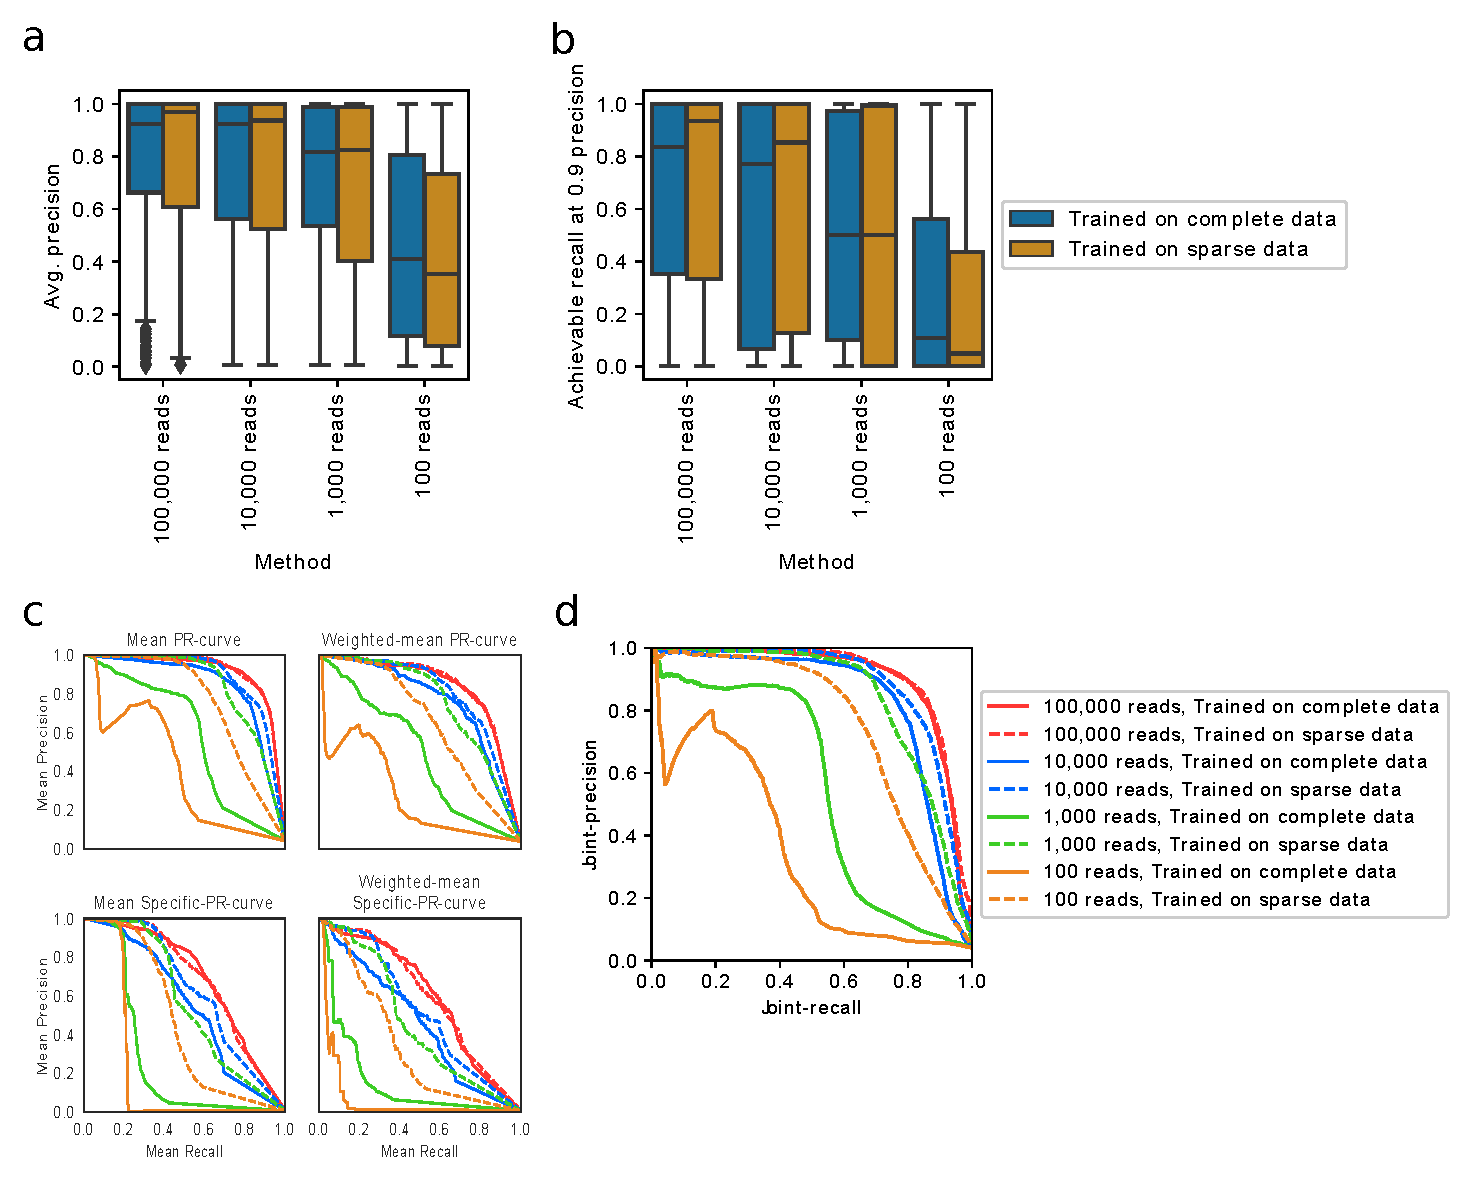
\includegraphics[width=13cm]{figures/bulk_train_and_test_downsampled_results.pdf}}
      \caption{\textbf{Results training on sparse training data and testing on sparse test set.} (a) Comparison between the distributions of average-precision generated by each method across all cell types.  (b) Comparison of the distributions over the highest chievable recalls when precision is fixed at 0.9 across all cell types. (c) Variants of the mean precision-recall curves for comparing the average performance of each method across all samples. (d) The joint-precision recall curves for all methods generated by ranking all sample-cell type output probabilities jointly.}
      \label{fig:results_train_and_test_bulk_downsample}
      \end{figure}

Next, we trained a classifier on a version of the complete bulk RNA-seq dataset (i.e. the union of the training and test sets) that was downsampled to 25,000 reads, which was the approximate number of reads in each 10x sample. We then applied the classifier trained on this downsampled data to the 10x data. As before, we found this classifier to outperform the classifier that was trained on the full, non-downsampled bulk RNA-seq training set (Fig.~\ref{fig:10x_results}).

\subsection{Testing on imputed, sparse scRNA-seq data}

Unfortunately, in order to improve the classifiers by training on sparse data, the sparsity of the training data should match the test data. This cannot be assumed as differing scRNA-seq datasets will often have differing read-depths. Therefore, we also explored an approach in which we train the classifiers on the full, bulk RNA-seq data and then apply them to sparse scRNA-seq data that has undergone gene expression imputation.  Because gene expression imputation requires pooling data across cells in a large collection of scRNA-seq data, this approach was not apt for application to the sparsified bulk RNA-seq dataset. Therefore, we only tested these methods on the 10x dataset.  Specifically, we trained one-vs.-rest cell type classifiers on the full set of bulk RNA-seq data using only the \NumTenXIntersection{} that also were present in the 10x dataset. Before testing these models on the 10x data, we imputed the expression of genes using MAGIC (\citealp{Dijk2018}), which uses a graph diffusion procedure on the single-cell nearest-neighbors graph.  We ran MAGIC in two modes of operation: an "optimistic mode" and a "realistic mode".  In the "optimistic" mode of operation, we ran MAGIC on each 10x PBMC cell type separately (i.e. we ran MAGIC separately on the data represented by each row of Table~\ref{tab:10x_pbmc}).  In this mode, only cells of the same cell type share information during the imputation process, thereby mitigating the possibility that the algorithm will incorrectly use cells of one cell type to impute the missing gene values within a cell of a differing cell type.  This mode of operation therefore provides results that serve as a sort of upper bound on the potential of gene expression imputation.  In the "realistic" mode of evaluation, we ran MAGIC on the entire PBMC dataset jointly, which better resembles how this tool is used in practice (i.e. the query data usually consists of heterogeneous cell types and information is potentially shared across cells from differing cell types).

Perhaps unsurprisingly, running MAGIC in the "optimistic" mode resulted in very high performance, which indicates that collectively, the cells contain the information for performing accurate classification, but that sparsity within a given cell makes classification difficult.  We also found that performing MAGIC in the "realistic" mode led to improvement over the application of the classifiers on the non-imputed data. 

 \begin{figure}[h!]
      \centerline{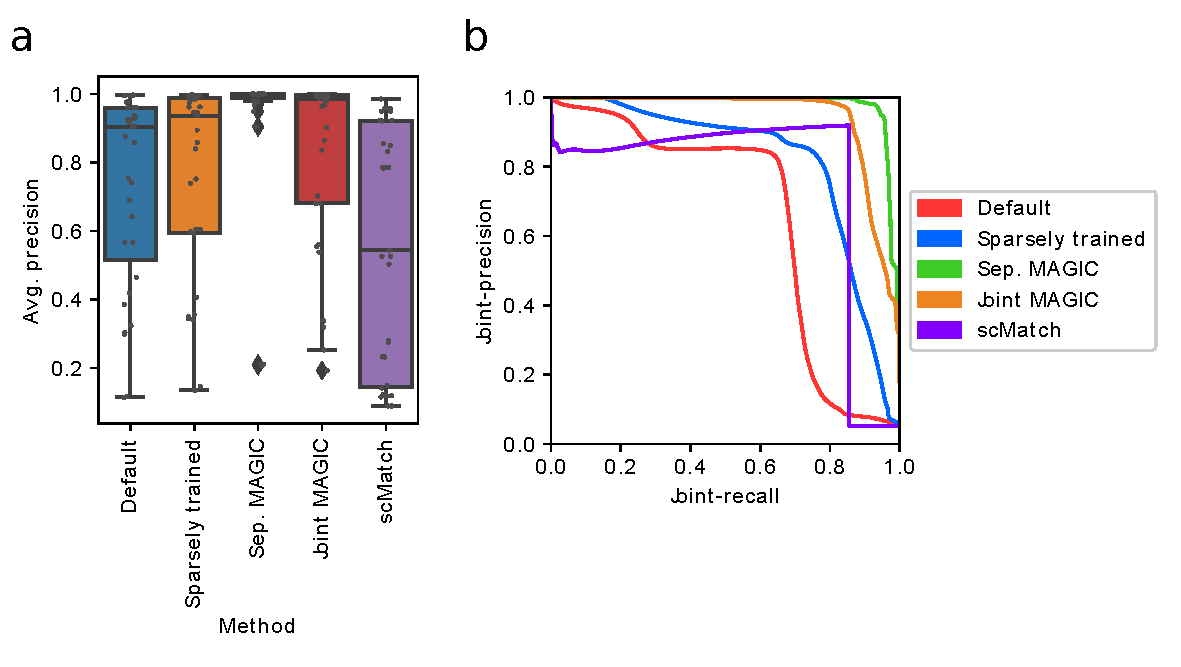
\includegraphics[width=13cm]{figures/10x_results.pdf}}
      \caption{\textbf{Results on 10x dataset.} (a) Comparison between the distributions of average-precision generated by each method across all cell types.  (b) Comparison of the distributions over the highest achievable recalls when precision is fixed at 0.9 across all cell types.}
      \label{fig:10x_results}
      \end{figure}

 \begin{figure}[h!]
      \centerline{\includegraphics[width=18cm]{figures/10x_pr_curves_on_graph.pdf}}
      \caption{\textbf{10x test set precision-recall curves.} Precision-recall curves for each cell type on the 10x scRNA-seq test dataset. Each node is colored according to which method yielded the highest average precision (red = default classifiers, blue = sparsely trained classifiers, green = running MAGIC on each separate cell type, orange = running MAGIC on the entire 10x dataset, purple = scMatch). The intensity of the color corresponds to the difference between the highest average-precision and the second highest average-precision achieved for that node.}
      \label{fig:10x_pr_curves}
      \end{figure}



\subsection{Baseline reference-based approach}

In reference-based classification, each cell's expression profile is queried against a set of bulk reference expression profiles. The cell is then assigned the cell type pertaining to the most similar sample in the reference set.  As a representative example of a reference-based classifier, we used a recent method called scMatch  (\citealp{Hou2019}). We ran scMatch with the default settings, which uses the FANTOM5 database (\citealp{Lizio2017}) as a reference set and uses Spearman correlation as the similarity metric.   We found the independent one-vs.-rest models trained in Chapter~\ref{chap:2} outperfomed scMatch in the per cell type mode of evaluation (Fig.~\ref{fig:10x_results}), but underperformed scMatch in the joint-evaluation. This indicates that scMatch tended to yield more accurate classifications on more general, and therefore more common, cell types (Fig.~\ref{fig:10x_pr_curves}). When preprocessing the test data with MAGIC, our classifiers outperformed scMatch on both the per cell type and joint modes of evaluation (Fig.~\ref{fig:10x_results}, Fig.~\ref{fig:10x_pr_curves}).


\subsection{A probabilistic generative model for cell type classification of sparse data}\label{sec:sc_new_model}

Because gene expression imputation algorithms must compute on the entire query set, these algorithms cannot be deployed in a situation that requires either parallelizing classification across cells or performing cell type classification in a streaming fashion where cell type classification is performed on one cell at a time independently from the rest of the cells.   To address this shortcoming, we propose a novel method for adapting the bulk RNA-seq-trained classifiers from Chapter~\ref{chap:2} that is based on a probabilistic model of the sparse scRNA-seq data-generating process.  In this model we treat the sparse RNA-seq expression profile as an observed random variable and posit that this sparse expression profile was ``generated" from an unobserved, dense RNA-seq expression profile.  In order to perform binary classification for a given cell type, we compute the marginal probability that the sample is of the given cell type conditioned on the sparse data.  We hypothesize that if we can accurately model the latent random variable representing the dense expression profile so that it resembles the bulk RNA-seq data on which the classifier was trained, then our classifier will more accurately predict the sample's cell type.  


\subsubsection{Model description}

To more rigorously describe the model, we will introduce some notation. Let $\bold{x} \in \mathbb{N}^G$ be the observed sparse RNA-seq expression profile, where $G$ is the number of genes, and $x_i$ is the read count for gene $i$.  Let $s := \sum_{i=1}^G x_i \times 10^{-6}$ be the scaled read-depth for the observed scRNA-seq sample. Let $\bold{y} \in \{0, 1\}^L$ be the cell type assignments for $L$ cell types. That is $y_i \in \{0, 1\}$ indicates whether the cell belongs to cell type $i$.  We let $\bold{z} \in \mathbb{R}^G$ be a latent, dense expression profile, in units of counts per million (CPM), from which $\bold{x}$ was generated.  Further, we assume that $\bold{z}$ was sampled from one of $K$ gamma distributions\footnote{As shorthand, for a multivariate random variable $\bold{X} \in \mathbb{R}^n$, $\bold{X} \sim \text{Gamma}(\bold{a}, \bold{b})$ denotes the joint distribution of $\bold{X}$ where each element $X_i$ is independent of the rest and distributed according to $X_i \sim \text{Gamma}(a_i, b_i)$. Similarly, $\bold{X} \sim \text{Poisson}(\boldsymbol{\lambda})$ denotes that the elements are independent and distributed according to $X_i \sim \text{Poisson}(\lambda_i)$}, indicated by the random variable $k \in [K]$. We let $\bold{A} \in \mathbb{R}_{+}^{K \times G}$ be the matrix of shape parameters and $\bold{B} \in \mathbb{R}_{+}^{K \times G}$  be the matrix of rate parameters for these $K$ mixture components where $\bold{a}_k$ and $\bold{b}_k$ are the shape and rate parameters respectively of the $k$th component. We let $\boldsymbol{\phi} \in [0,1]^K$, where $\sum_{i=1}^K \phi_i = 1$, be the prior probabilities of drawing a sample from each mixture component.  We use $\sigma(x)$ to denote the logistic function:
$$\sigma(x) := \left[1 + \exp(-x)\right]^{-1}$$
Then, the full data-generating process (Fig.~\ref{fig:sc_graphical_model}) is as follows:
\begin{enumerate}
\item $k \sim \text{Categorical}(\boldsymbol{\phi})$
%\item For each gene $i \in [G]$:
\item $\bold{z} \sim \text{Gamma}(\bold{a}_k, \bold{b}_k)$
\item $\bold{x} \sim \text{Poisson}\left(\bold{z}s\right)$
\item For each cell type $i \in [L]$:
\begin{itemize}
\item $y_i \sim \text{Bernoulli}\left(\sigma\left(\boldsymbol{\beta}_i^T \log(\bold{z}+1)\right)\right)$
\end{itemize}
\end{enumerate}
To make a prediction for cell type $i \in [L]$, we compute the marginal probability of the cell type assignment $y_i$ conditioned on the observed, sparse data $\bold{x}$:
\begin{align*}
p(y_i=1 \mid \bold{x}) &= \sum_{k=1}^K \int_{\bold{z}} p\left(y=1 \mid \bold{z}\right) p\left(\bold{z} \mid \bold{x}, k\right) p\left(k \mid \bold{x}\right) \ d\bold{z} \\
&= \sum_{k=1}^K p(k \mid \bold{x}) E_{\bold{z} \mid \bold{x}, k} \left[p\left(y=1 \mid \bold{z}\right)\right]
\end{align*}
where 
$$p\left(y=1 \mid \bold{z}\right) = \sigma\left(\boldsymbol{\beta}_i^T\log(\bold{z}+1)\right)$$
and
$$\bold{z} \mid \bold{x}, k \sim \text{Gamma}(\bold{x}+\bold{a}_k, \bold{b}_k + s)$$
and 
$$p(k \mid \bold{x}) = \frac{ \phi_k \prod_{i=1}^G f_{\text{NegBin}}\left(x_i ; a_{k,i}, \frac{s}{s + b_{k,i}} \right)}{\sum_{k'=1}^K \phi_{k'} \prod_{i=1}^G f_{\text{NegBin}}\left(x_i ; a_{k',i}, \frac{s}{s + b_{k',i}} \right)}$$
where
$$f_{\text{NegBin}}(x; r, p) := \frac{\Gamma(x + r)}{x! \Gamma(r)} p^x(1-p)^r$$ 
is the probability density function for the Negative Binomial distribution, and
$$\Gamma(x) := \int_{0}^{\infty} z^{x-1}e^{-z} dz,$$
is the gamma function  (See Appendix~\ref{app:model_deriv} for full derivation of these probabilities).  

 \begin{figure}[h!]
      \centerline{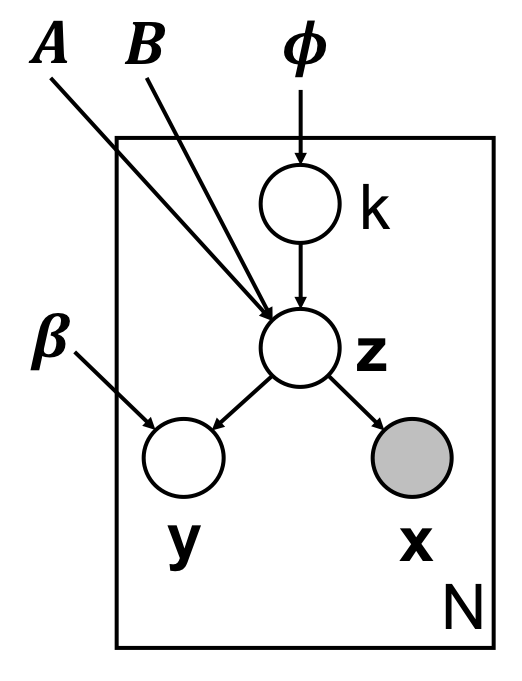
\includegraphics[scale=0.65]{figures/sc_graphical_model.png}}
      \caption{\textbf{Graphical model for sparse cell type classification.} The probabilistic graphical model for performing cell type classification on sparse RNA-seq data represented in plate notation.}
      \label{fig:sc_graphical_model}
      \end{figure}

\subsubsection{Model training and inference}

This model requires the specification of the gamma-mixture distribution over the latent, dense expression profile $\bold{z}$.  Specifically, we must specify the gamma shape and rate parameters, $\bold{A} \in \mathbb{R}^{G \times K}$ and $\bold{B} \in \mathbb{R}^{G \times K}$ respectively, for all K clusters.  As a first approach to specifying this distribution, we propose a two-step process that entails first clustering the bulk RNA-seq training data and then using each cluster to estimate a joint distribution over the CPM values for each gene where each gene is independent and gamma-distributed.    This process introduces a number of modeling choices in regards to which clustering algorithm to deploy as well as how each gamma distribution is to be estimated.

When applying the trained model to query data, one must compute $p(y_i=1 \mid \bold{x})$, which requires the calculation of an expectation. Unfortunately, this expectation does not admit a ready closed-form solution.  Instead, it must be approximated either through Monte Carlo integration\footnote{Monte Carlo integration of an expectation $E(f(X))$ involves sampling $n$ samples $x_1,\dots,x_n \overset{\text{i.i.d.}}{\sim} X$ and then approximating the expectation via $\frac{1}{n}\sum_{i=1}^n f(x_i)$. } or through an analytical approximation.  For the remainder of this chapter, we deployed Monte Carlo integration, finding that the variance of the expectation was low with 100 samples.  Future work will entail developing an accurate analytical approximation.

\subsubsection{Relationship to existing approaches}

We note that the model presented in this chapter has similarities to recent bulk RNA-seq-informed gene expression imputation algorithms.  Specifically, SCRABBLE (\citealp{Peng2019}) and URSM (\citealp{Zhu2018}) were developed to utilize a bulk RNA-seq dataset to inform the value of missing genes in the target scRNA-seq data.  SCRABBLE sets up an optimization problem in which the goal is to find a dense representation of the scRNA-seq dataset for which the aggregate of the imputed expression profiles most closely resembles the bulk RNA-seq data.  In contrast, URSM is more related to the model proposed in this chapter in that URSM also proposes a joint probabilistic model over both the scRNA-seq data as well as the bulk RNA-seq data.  Importantly both SCRABBLE and URSM assume that that the bulk RNA-seq sample provided as input to the imputation algorithm represents a mixture of the cell types present in the target scRNA-seq dataset. Therefore, these methods are most apt for scenarios in which a bulk RNA-seq sample can be obtained from the same biological sample as that from which the scRNA-seq sample was obtained.  In this chapter, this assumption cannot be made as we seek to leverage the trove of heterogenous, publicly available bulk RNA-seq data.

We also point out similarities between this model and the SAVER algorithm for gene expression imputation (\citealp{Huang2018}). To perform imputation, SAVER assumes a similar gamma-poisson generative process of the scRNA-seq data where each cell is generated by first sampling a rate parameter from a gamma distribution and then sampling the counts from a Poisson distribution using the gamma-sampled rate. However, SAVER differs from the approach discussed here in a few fundamental ways: first, in SAVER the gamma parameters are learned from the scRNA-seq data itself, rather than from a bulk RNA-seq training set. Second, each cell in the dataset is associated with a unique gamma-prior over the Poisson rate parameter where the parameters of each cell's gamma-prior are estimated from the non-zero count genes in the cell via a regression model.  Because this regression model is trained using the full scRNA-seq dataset, this method is principally more similar to other gene expression imputation algorithms, like MAGIC, that rest on pooling data across cells.

 \subsubsection{Demonstration on toy data}
 
 To demonstrate this model, we ran this model in a toy setting in which there exist only two gamma mixture components corresponding to two cell types: primordial germ cells and CD8-positive alpha-beta T cell. We use all of the bulk RNA-seq data for these two cell types to estimate the two gamma distributions using the method of moments method. We then tested the ability of our proposed generative model to modify the performance of the bulk RNA-seq-trained classifier for the "lymphocyte" cell type.  We tested this model on two single-cell samples from the scRNA-seq dataset described in Chapter~\ref{chap:2}.  Specifically, we used one cell labelled as CD8-positive alpha-beta T cell  (SRA accession SRX1461628) and another single cell labelled as primordial germ cell (SRA accession SRX1658583).  We downsampled the reads from these two single-cell samples at read-depths of $10^6$, $10^5$, $10^4$, $10^3$, 100, and 10 reads. We generated a total of 10 expression profiles for each read-depth, and the ran the model on each of these expression profiles.  Specifically, we compared the output probability of the standard lymphocyte classifier (i.e. without the generative model component) to the generative model's output probability for these two samples across each expression profile.  Since "lymphocyte" is an ancestor of "CD8-positive alpha-beta T cell" in the ontology, but is unrelated to "primordial germ cell", we would expect the classifier to assign the CD8-positive alpha-beta T cell a high probability of being a lymphocyte across all read-depths and to assign the primordial germ cell a low probability of being a lymphocyte across all read-depths. 
 
As expected, we found the standard lymphocyte classifier to be poorly calibrated at low read-depths, assigning the CD8-positive alpha-beta T cell a very low probability of being a lymphocyte. However, under the generative model, the cell is given a high probability of being a lymphocyte (Figure~\ref{fig:sc_model_toy_experiment}).   Although the new model gives higher probability that the primordial germ cell is a lymphocyte at 10 reads, as the read-depth increase, the probability of being a lymphocyte quickly decreases towards zero. In contrast, even at $10^3$ reads, the default classifiers outputs non-zero probability that the cell is a lymphocyte. Lastly, we see that as the read-depth increases the probabilities output by both the generative model and the default classifier converge.  This is due to the fact that as the read-depth increases, the data better resembles the bulk RNA-seq data on which the classifier was trained. Similarly, as the read-depth increases, the prior plays a smaller role in the generative model and the classifier approximately operates on the observed expression profile.  
       
 \begin{figure}[h!]
      \centerline{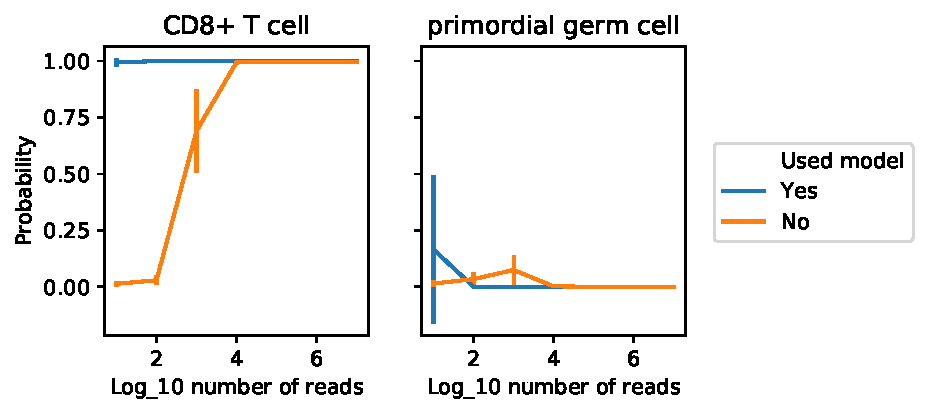
\includegraphics[width=13cm]{figures/downsample_apply_sc_model.pdf}}
      \caption{\textbf{Illustration of advantage of probabilistic model.} Results from the toy two-cell experiment demonstrating the potential advantages of this model. At each read-depth, 10 samples were generated from the CD8+ T cell sample (left) and the primordial germ cell sample (right).  At each read-depth, we plot the mean probability output by the default lymphocyte classifier (orange) and the mean probability output by the generative model-based lymphocyte classifier (blue) across the 10 samples. Error bars denote plus and minus one standard deviation around the mean.}
      \label{fig:sc_model_toy_experiment}
      \end{figure}
      
 \subsubsection{Performance on sparsified bulk RNA-seq test data}
 
 We evaluated this model by training it on the bulk RNA-seq training set and applying it to the sparsified versions of the bulk RNA-seq test set.  We explored a number of approaches for specifying the gamma-mixture distribution over the latent random variable $\bold{z}$, which entailed a number of clustering algorithms algorithms and methods for estimating the gamma parameters in each mixture component.  Specifically, we tested three clustering algorithms: agglomerative clustering with Pearson correlation distance using 500 clusters, using each cell type in the training set to define clusters, and finally, clustering the data \textit{within} each cell type and using the union of all clusters within all cell types.  We also tested two methods for estimating the parameters of each gamma distribution from the samples within each corresponding cluster: In the first variant, we use method of moments. In the second variant, we fit the mean using method of moments, but then perform an empirical Bayes-like approach to increase the variance when variance is low (thereby "smoothing" the gamma distributions).  We found that these various methods for estimating the gamma distributions yielded qualitatively similar performance and report here the best performing variant: using each cell type in the training data to define a cluster and performing the empirical Bayes-like procedure (Appendix~\ref{app:model_deriv}). 
 
In the per-cell type mode of evaluation, we found that this model tended to underperform the default classifiers at most read-depths, except the lowest (100 reads per sample).  Examining the performance across cell types, we found that the model severely underperformed in certain sections of the ontology.  For example, the model tended to perform poorly on epithelial cells, but comparably on lymphocytes (Fig.~\ref{fig:diff_cell_types}).  It is likely that this is due to the fact that the gamma distributions for these cell types are poorly fit. Future work will require further diagnosing the model in order to improve performance on these underperforming cell types. Because of the lower performance on many cell types, we decided to forego testing this model on the 10x dataset until future work could be carried out that would improve performance on these underperforming cell types.  By decreasing the number of times we evaluate this model on the 10x dataset, we mitigate the likelihood that modifications to the algorithm in response to the results will lead to overfitting on this dataset.

Nonetheless, when examining the performance in the per-sample and joint-modes of evaluation we find that this model produces better results than the default classifiers on all read-depths except the highest ($10^5$ reads per sample), which indicates two things. First, on common cell types, the model performs well, and second, the output probabilities of this model are much better calibrated across cell types than the default classifier's.  These results support our hypothesis that by imputing the genes, the input data better matches the data on which the models were trained and therefore calibrated.  Thus, this model offers a promising approach to scRNA-seq cell type classification, especially at extremely low read-depths. 

  \begin{figure}[htbp]
\centering
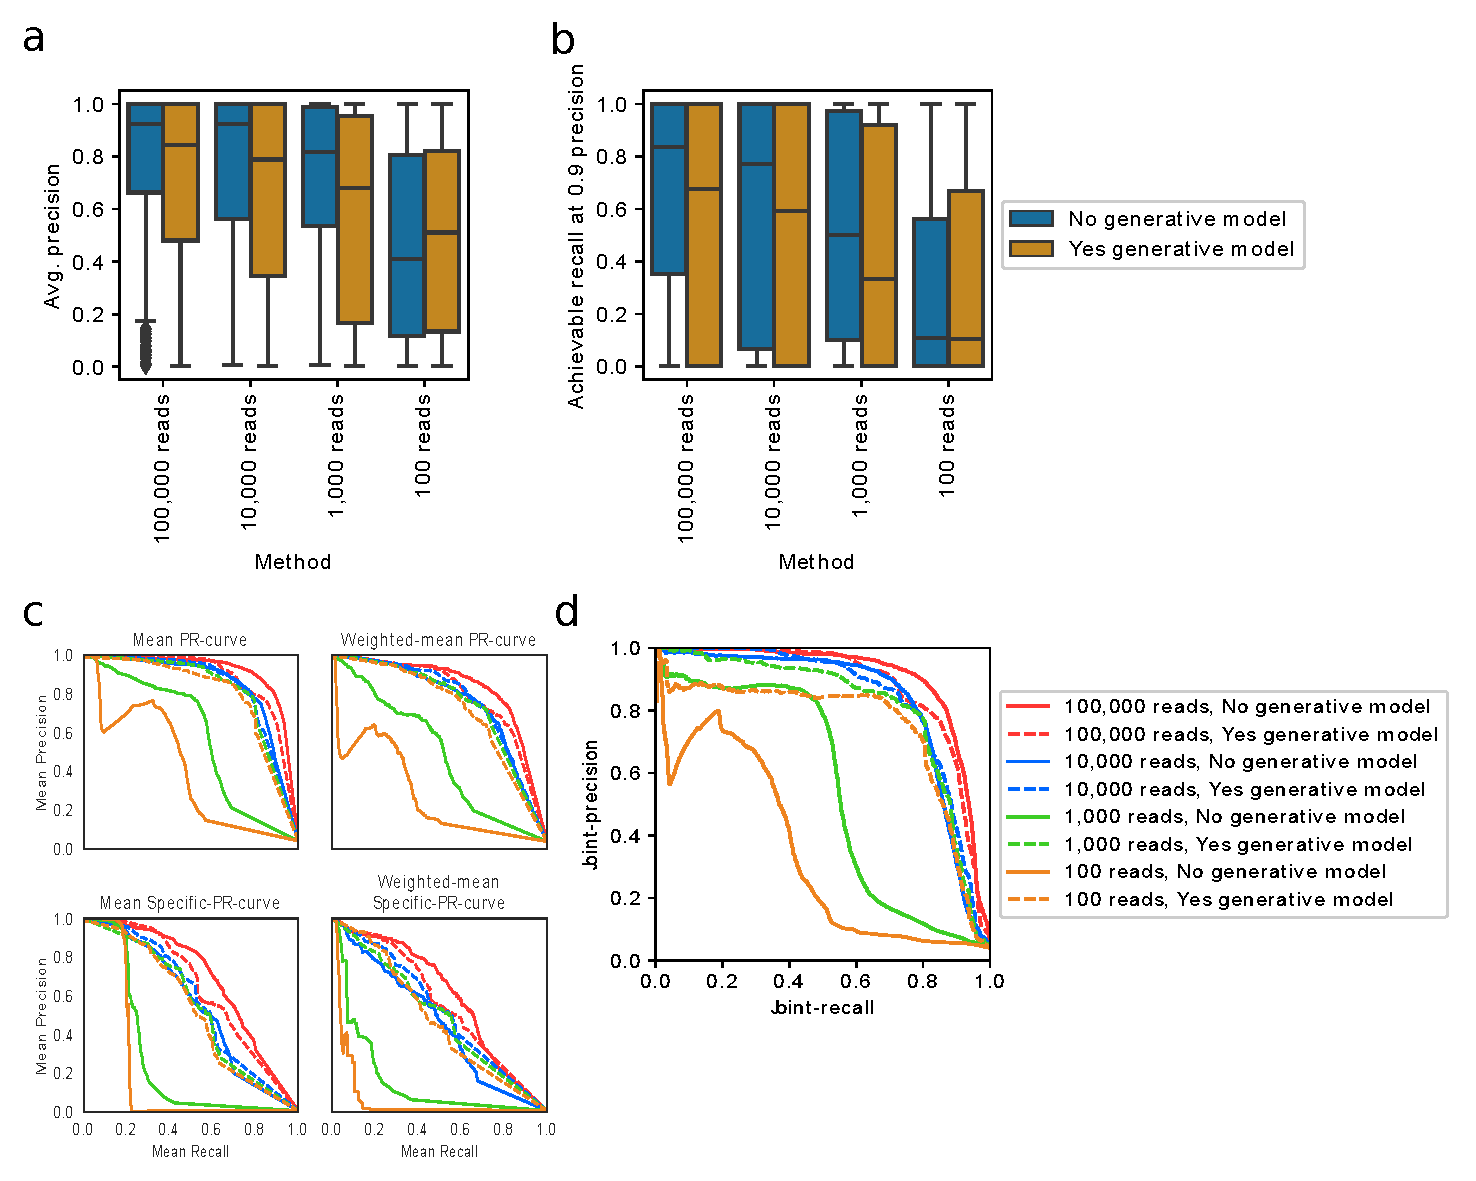
\includegraphics[width=13cm]{figures/new_model_results.pdf}  
\caption{\textbf{Results of the new model on the downsampled bulk RNA-seq test set.} (a) Comparison between the distributions of average-precision generated by each method across all cell types.  (b) Comparison of the distributions over the highest achievable recalls when precision is fixed at 0.9 across all cell types. (c) Variants of the mean precision-recall curves for comparing the average performance of each method across all samples. (d) The joint-precision recall curves for all methods generated by ranking all sample-cell type output probabilities jointly.}
\label{fig:diff_cell_types}
\end{figure}
 
 \begin{figure}[htbp]
\centering
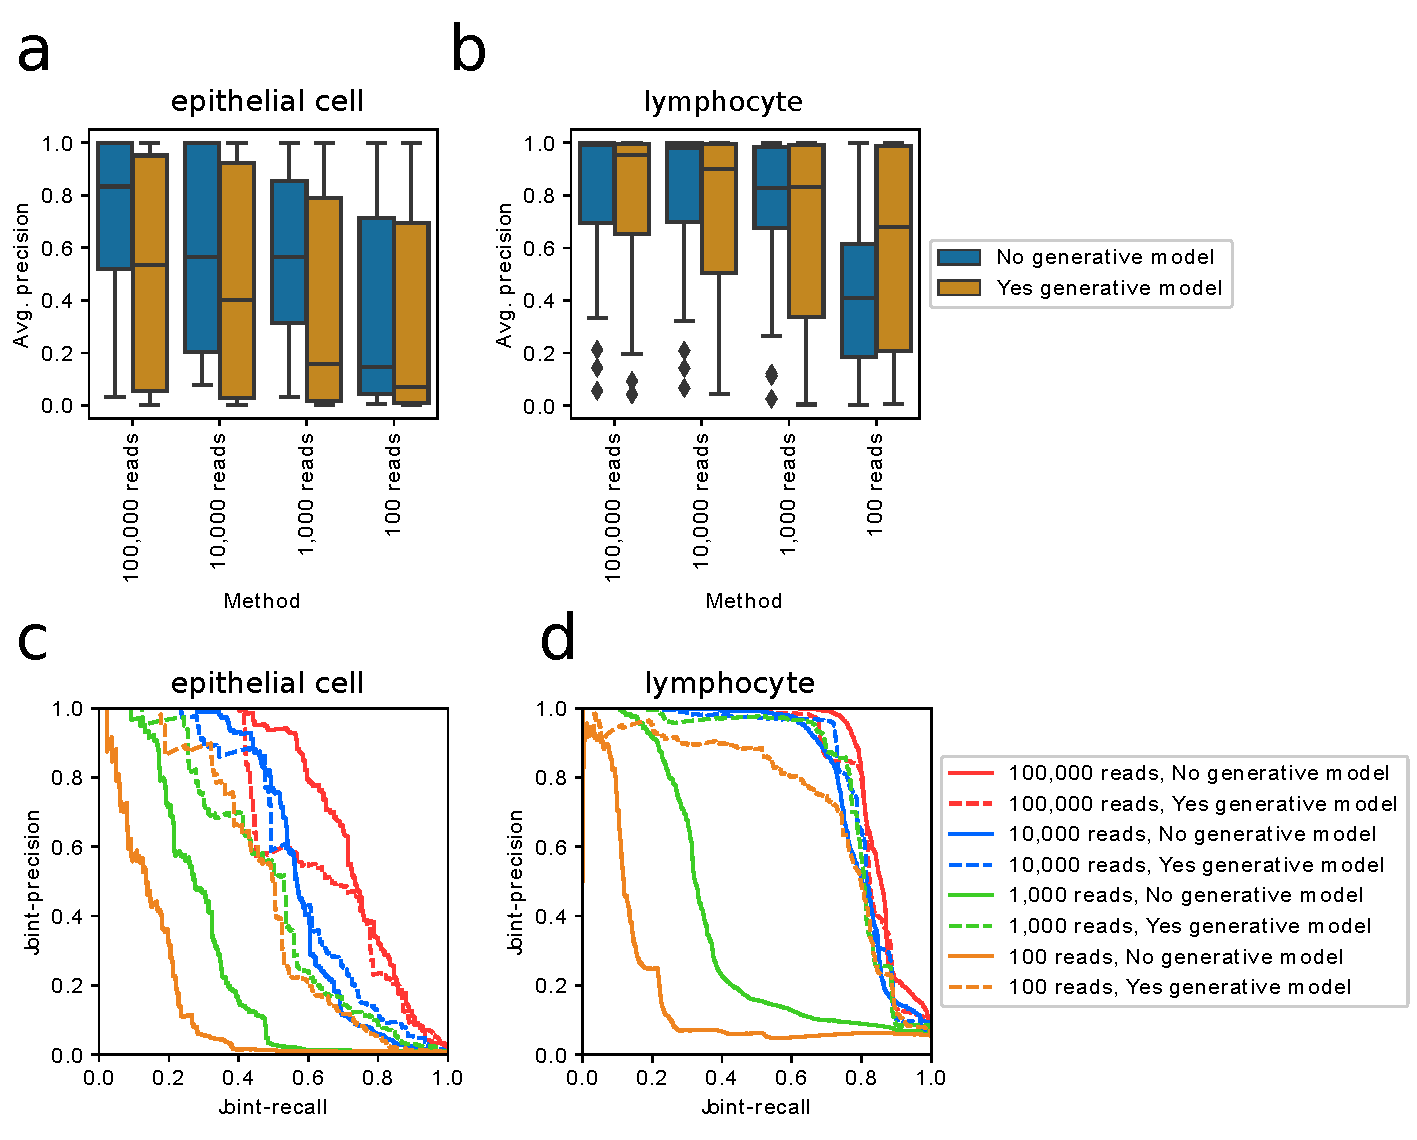
\includegraphics[width=13cm]{figures/paired_avg_precision_two_cell_types}  
\caption{\textbf{Performance of new model on differing sections of the ontology.} Comparing the distribution of average precision scores across cell types between the standard classifiers and the classifiers adapted with the probabilistic model. We compare the distributions across (a) epithelial cell types and (b) lymphocyte cell types. We also compare the join-precision-recall curves for (c) epithelial cell types and (d) lymphocyte cell types.}
\label{fig:diff_cell_types}
\end{figure}
 
%\subsubsection{Diagnosing the model}
      
\subsection{Conclusions and future work}

In this work, we explored approaches for extending the one-vs.-rest cell type classifiers developed in Chapter~\ref{chap:2} to sparse scRNA-seq data. Because these classifiers were trained on bulk RNA-seq data, they performed poorly on sparse data out of the box.  To address these shortcomings we explored methods for imputing the values for the genes in order for the test data to better resemble the dense training data.

To address these shortcomings, we explored two main approaches for adapting the classifiers developed in Chapter~\ref{chap:2}:
\begin{enumerate}
\item Training on artificially sparse bulk RNA-seq data in order for the training data to better resemble the sparse test data.
\item Imputing the values for the genes in order for the test data to better resemble the dense training data.
\end{enumerate}
When possible, we evaluated each strategy on both an artificially sparse bulk RNA-seq test set as well as a dataset of droplet-based 10x scRNA-seq expression profiles consisting of various peripheral blood mononuclear cell types. 

Unsurprisingly, we found that training on artificially sparse bulk RNA-seq data led to better performance than the default, out-of-the-box classifiers.  However, this gain in performance requires training a classifier at a read-depth that matches the test set. Since our goal is to train a single classifier for use on scRNA-seq datasets of varying read-depths, we explored the use of gene expression imputation algorithms that would enable training the classifier only once. We found that imputing the values of the genes with MAGIC led to improved performance.  This indicates that pre-processing the query data with a gene expression imputation algorithm will improve the results of cell type classifiers trained on bulk RNA-seq data.  Future work will involve benchmarking other recent imputation algorithms, such as SAVER, for the cell type classification task. 

 Lastly, because gene expression imputation requires expensive computation at test-time, we explored a novel method for classification of sparse scRNA-seq data based on a generative model of the scRNA-seq data-generating process. This model outperformed the default classifiers on the per-sample and joint-modes of evaluation.  Most promisingly, at very low read-depths, this model provided results that were competitive with those from higher read-depths. Nonetheless, we found that the model suffered on certain cell types. Future work will require diagnosing the cause for the poorer performance on these cell types. Nonetheless, these results reveal a promising direction towards the goal of developing a robust, well-calibrated classifier for classifying sparse scRNA-seq data against the full breadth of the Cell Ontology.  


 






\chapter{Conclusion and future work } \label{chap:future}

Transcriptome-based cellular phenotyping (TBCP) is a task with a number of important applications in biology and medicine.  The trove of publicly available RNA-seq data promises to be a valuable source of data for training machine learning algorithms to perform TBCP; however, to date utilizing the SRA for this purpose has remained challenging.  In this dissertation, we presented three bodies of work that progress our ability to utilize this data for training TBCP algorithms.  These projects make contributions across the machine learning pipeline. 

 In Chapter~\ref{chap:1}, we presented the MetaSRA, a novel computational pipeline and associated database for labelling phenotypes in the poorly structured metadata of the SRA.  Our approach extended named entity recognition (NER) to not only label samples using mentioned terms, but also inferred which mentioned terms actually describe the biology of the sample. We found that our approach was able to produce results with similar levels of recall as state-of-the-art NER methods, but contained far fewer errors. 
  
 In Chapter~\ref{chap:2}, we leveraged the standardized phenotype labels produced by the MetaSRA to supervise the training of cell type classifiers.  We advocate the use of hierarchical classification to make full use of the graph-structure of the ontologies. To this end, we applied ensemble-based hierarchical classification algorithms to the cell type classification task and pushed the state-of-the-art in hierarchical cell type classification performance.  
 
In Chapter~\ref{chap:3} we explored methods for extending the classifiers trained in Chapter~\ref{chap:2} to sparse, single-cell RNA-seq data generated from novel droplet-based technologies. We found that methods for imputing the values of each gene increased the classification performance of the trained classifiers. Further, we introduced a novel probabilistic model for implicitly performing gene expression imputation based on bulk RNA-seq data, which offers a promising approach to cell type classification in settings where computational resources and time are limited, such as clinical settings.

In the subsections below, we discuss general areas that deserve further investigation.

\subsection{Applications to other phenotyping tasks}

Although the MetaSRA produced standard phenotype labels for multiple categories of phenotypes including disease, cell type, tissue, and cell line, the majority of the work presented in this dissertation regarding the actual training of machine learning algorithms focused on the cell type classification task. However, the methods that we explored are applicable to other phenotyping tasks as well. For example, the hierarchical classification algorithms explored in Chapter~\ref{chap:2} can be applied to disease type classification using the Disease Ontology. 

\subsection{Quantifying and leveraging label-uncertainty}

The methods used in the MetaSRA ontology term mapping process do not take into account uncertainty and therefore do not output a confidence for each mapped ontology term.  A confidence score associated with each mapped ontology term would prove useful for users in that it would enable users to set a confidence threshold in their MetaSRA-enabled queries of the SRA.  Intuitively, there are a number of signals that the MetaSRA could feasibly use to calculate this confidence score. For example, the MetaSRA should be less certain about an ontology term that is mapped to the sample due to a fuzzy string match with the metadata than it should be about a term that exactly matches the metadata.  

In a similar vein, the classifiers developed in Chapter~\ref{chap:2} use the training labels as ground-truth and are not equipped to handle the possible uncertainty in those labels.  Because of this, a manual curation effort was required to remove cell type labels in the training set that were incorrectly mapped by the MetaSRA. If these labels were instead associated with a confidence score, methods could be pursued to train phenotype classifiers that take into account uncertainty in the training data. 

\subsection{Interpreting the trained models}

In Chapter~\ref{chap:2}, we advocate the use of linear models for classification, in part, due to their relative interpretability in comparison to other modeling frameworks (such as neural networks).  Linear models are interpretable in so far as the magnitude of each feature's coefficient reflects that feature's impact on the classifier's decision.  Nonetheless, because these models use so many features (i.e. one per gene) important questions remain as to how many genes are being used in a meaningful way by each cell type classifier.  Such an investigation may shed light on whether cell types are predominantly defined by relatively few distinguishing genes, or rather, by more global expression changes across the genome.


\begin{appendices}
\chapter{Detailed descriptions of the metadata normalization procedures }\label{app:1}

\section{Detailed description of ontology term mapping pipeline } \label{sec:mapping_pipeline}

\begin{enumerate}
\item \textbf{Initializing the Text Reasoning Graph (TRG):} The initial TRG consists of a set of nodes that represent the raw set of key-value pairs describing the sample.  First, a node is created for each key-value pair.  From each of these ``start nodes'', we draw two edges to two artifact nodes -- one artifact representing the key and the other artifact representing the value.  Figure~\ref{fig:init_trg} depicts the initial TRG for the following set of key value pairs:
\begin{align*}
    &\text{\texttt{cell line: Parkin-expressing MRC5 fibroblasts}}\\
    &\text{\texttt{cell state: Proliferating}}\\
    &\text{\texttt{source\_name: Prolif}}
\end{align*}

\begin{figure}[htbp]
\centering
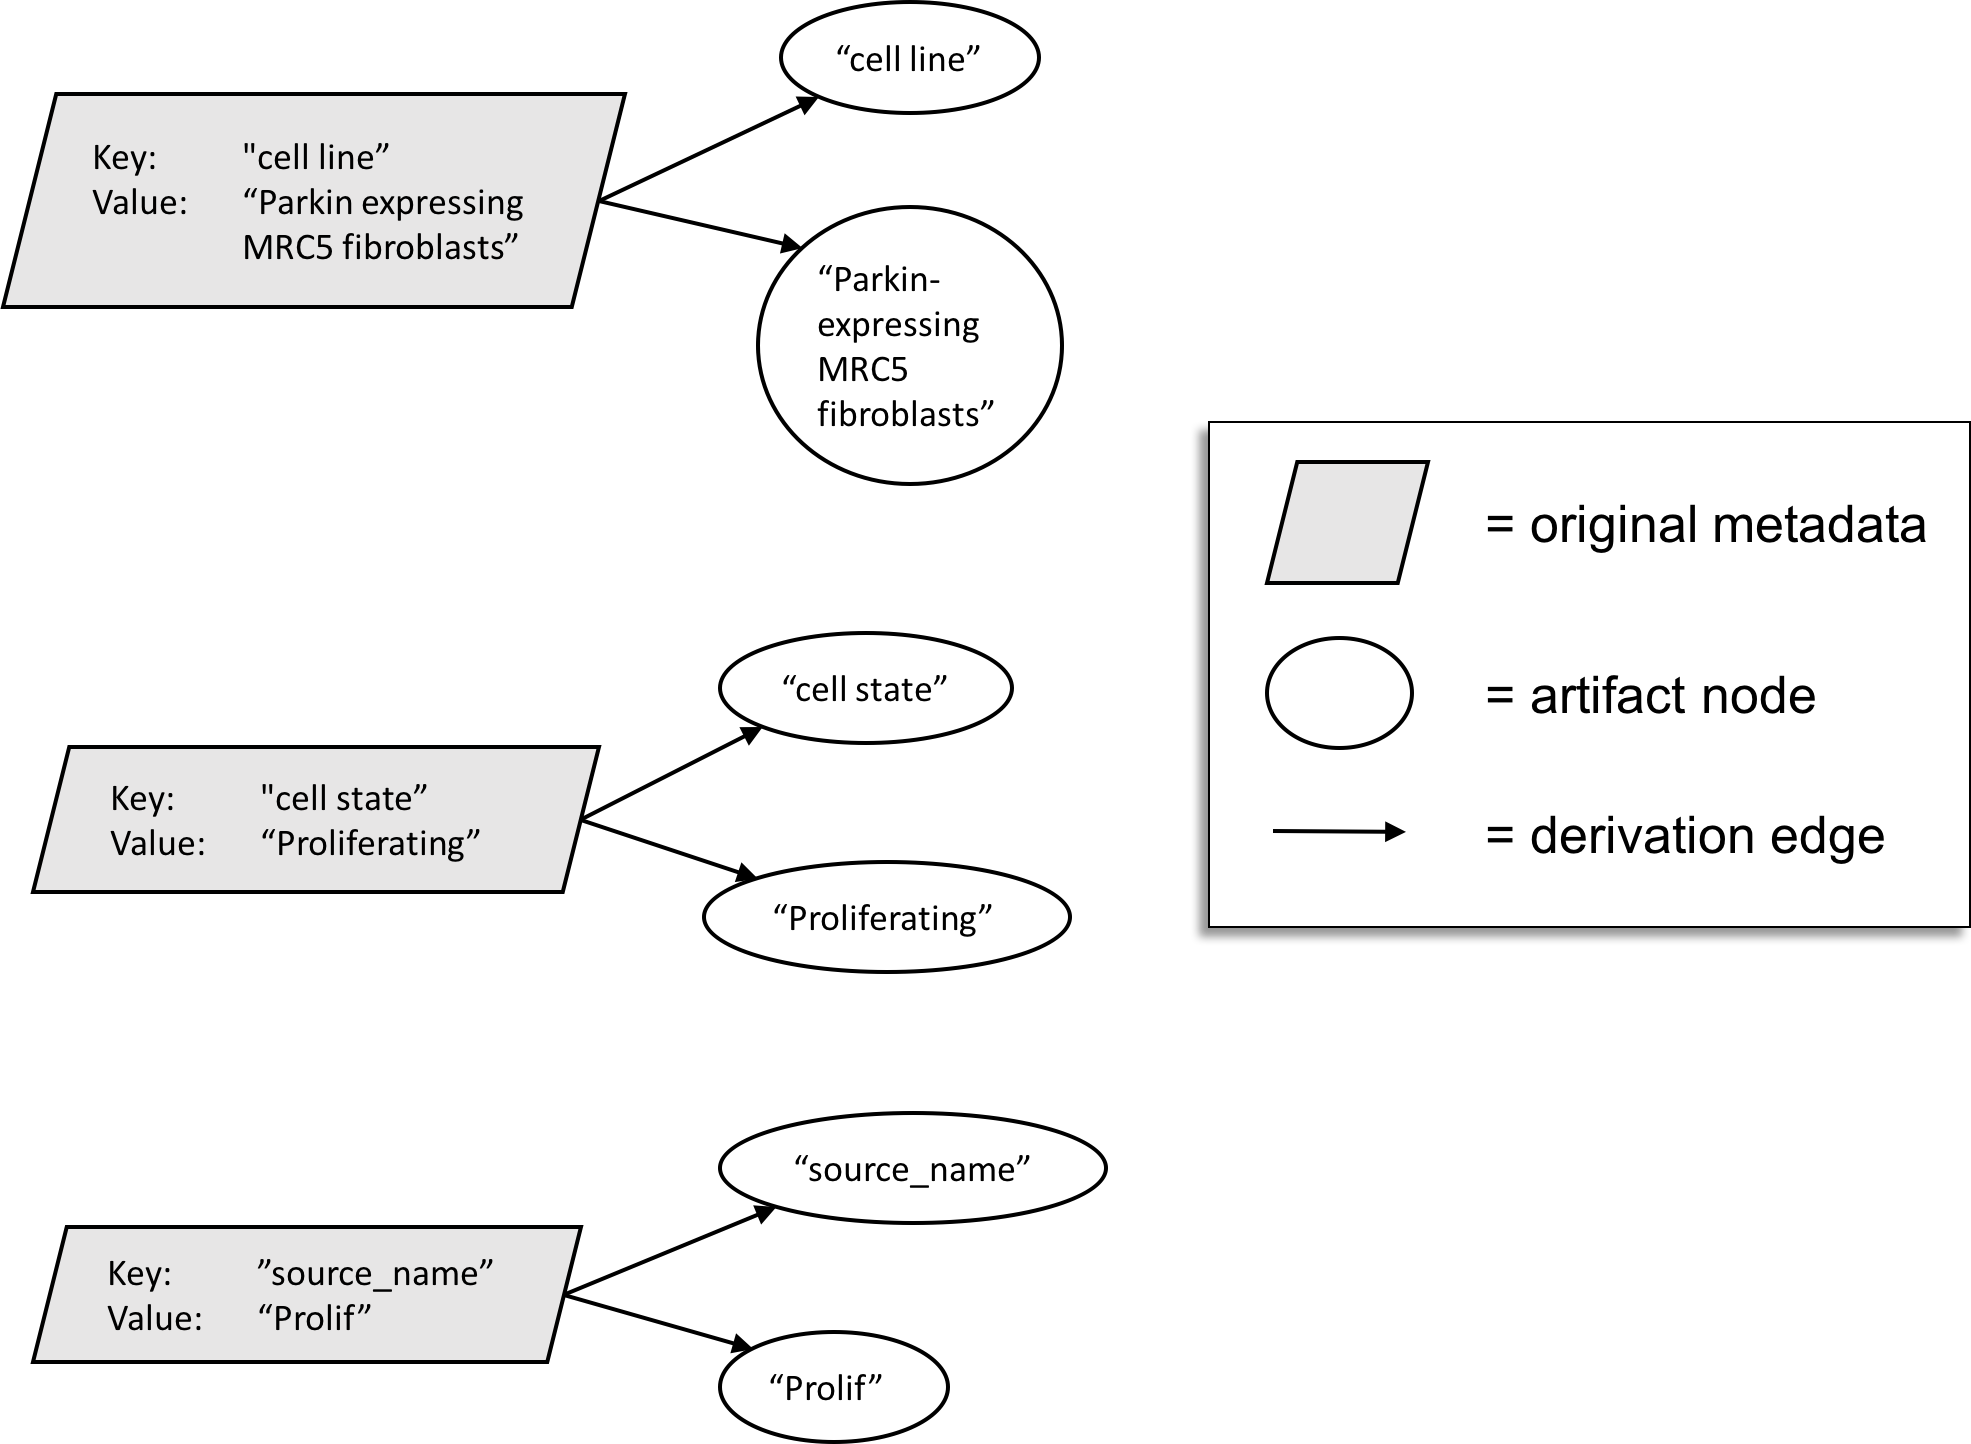
\includegraphics[width=13cm]{figures/init_trg.png}  
\caption{\textbf{Initial TRG.} The initial TRG created from a set of key-value pairs describing a sample.}
\label{fig:init_trg}
\end{figure}

\item \textbf{Generating $n$-grams:} From each artifact node, we generate all $n$-grams for $n = 1,\dots,8$. We use the Python Natural Language Toolkit (nltk) to tokenize the text before constructing $n$-grams.  For each $n$-gram generated from an artifact, we draw an edge from the original artifact to the derived artifact. Figure~\ref{fig:stages_1}A illustrates an artifact node from the graph of Figure~\ref{fig:init_trg} with derived artifacts representing $n$-grams. 

\begin{figure}[htbp]
\centering
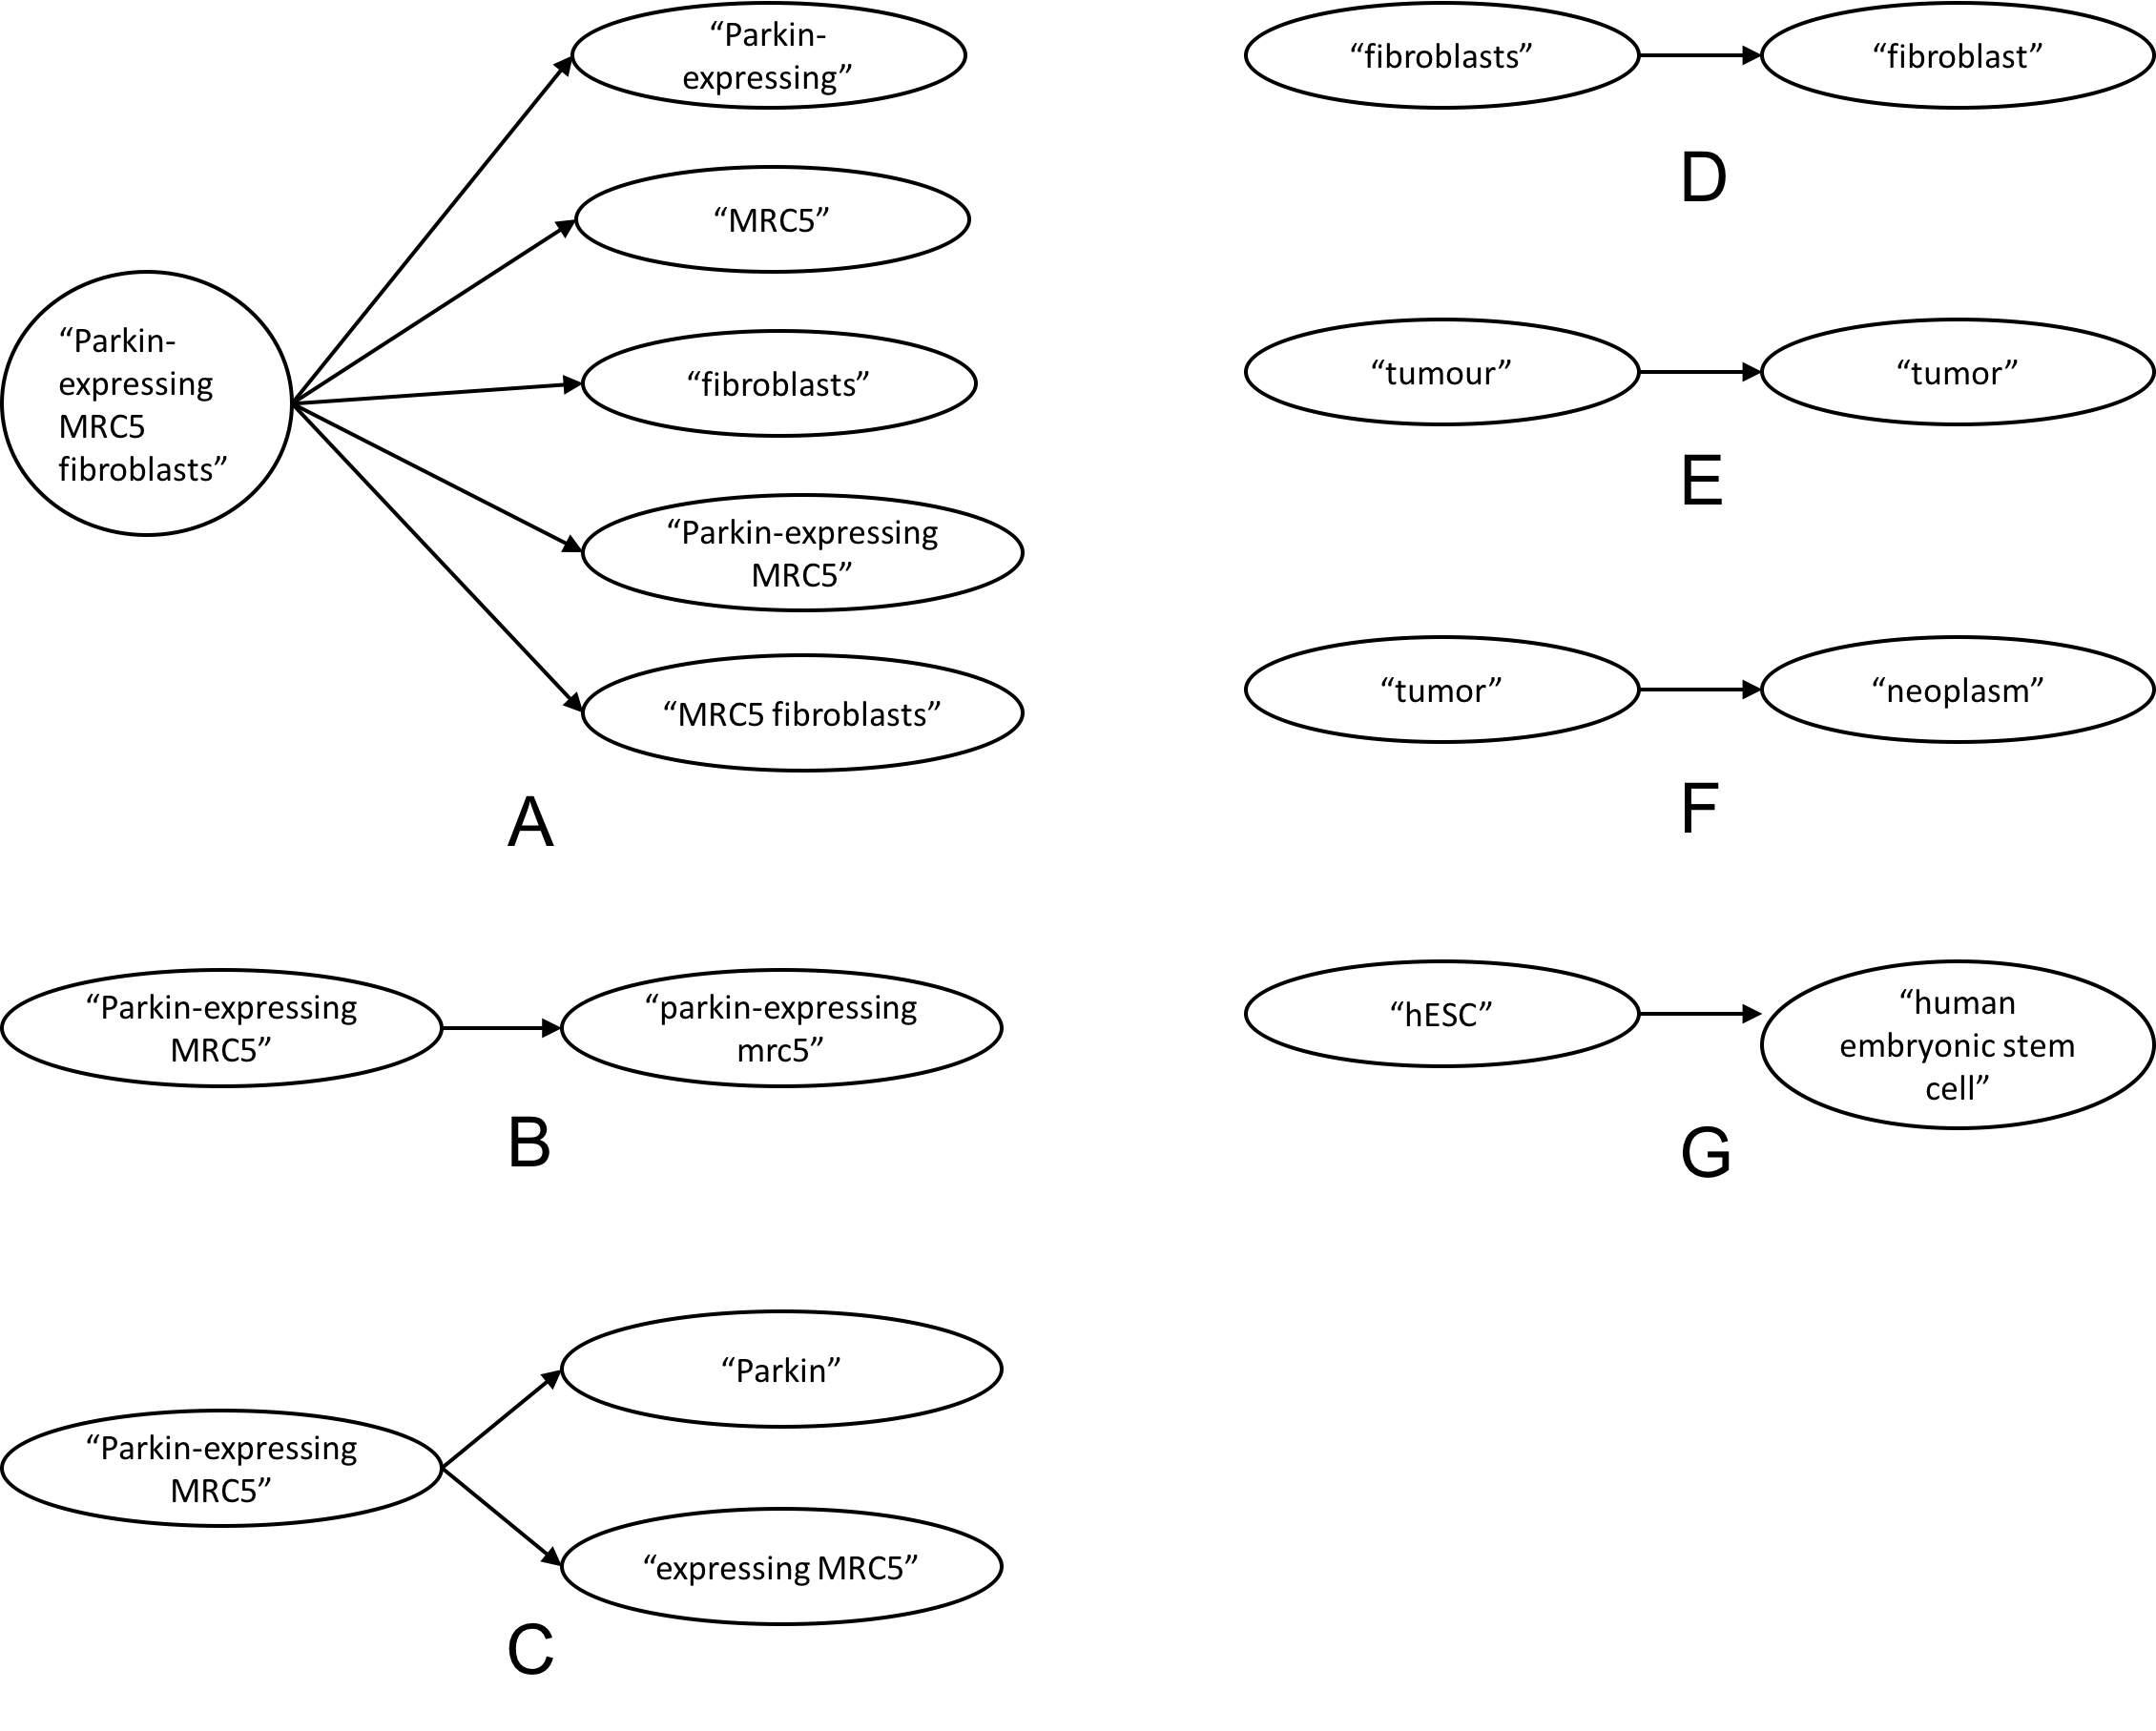
\includegraphics[width=13cm]{figures/stages_1.png} 
\caption{\textbf{Artifact derivations.} (A) An artifact node with derived $n$-grams. (B) An artifact with a derived lowercase artifact. (C) Delimiting artifacts on special characters. (D) Deriving inflectional variants. (E) Deriving spelling variants. (F) Deriving custom synonyms. (G) Expanding acronyms.}
\label{fig:stages_1}
\end{figure}

\item \textbf{Lowercase:} From each artifact node that represent artifacts with uppercase characters, we draw an edge to a new artifact node that has all lowercase characters. Figure~\ref{fig:stages_1}B demonstrates this process.

\item \textbf{Delimiters:} The NLTK's tokenizer does not split on the characters ``+'', ``-'', ``/'', and ``\_''.  We therefore, split all artifact strings by these delimiters as shown in Figure~\ref{fig:stages_1}C.  

\item \textbf{Inflectional variants:} We derive the inflectional variants of all artifacts by consulting the SPECIALIST Lexicon. This is demonstrated in Figure~\ref{fig:stages_1}D.

\item \textbf{Spelling variants:} We derive the spelling variants of all artifacts by consulting the SPECIALIST Lexicon. This is demonstrated in Figure~\ref{fig:stages_1}E.

\item \textbf{Manually annotated synonyms:} There are certain words that are very common in the metadata, but that are not included in the ontologies. For example, the word ``tumor'' is extremely common in the metadata, but is not present in the Disease Ontology. We filled such gaps by creating a small, custom thesaurus.  In our thesaurus, ``tumor'' is given the synonym ``neoplasm.'' The word ``neoplasm'' is a term in the Disease Ontology that is semantically equivalent to ``tumor.''  This process is demonstrated in Figure~\ref{fig:stages_1}F.

\item \textbf{Custom acronym expansion:} There are certain acronyms that are common in the metadata, but are not included in the ontologies. For example, the acronym ``hESC'' is very common in the metadata, but is not present in the Cell Ontology.  We filled such gaps by expanding common acronyms. For example, we expand ``hESC'' to ``human embryonic stem cell.'' This process is demonstrated in Figure~\ref{fig:stages_1}G.  

\item \textbf{Exact string matching:} We perform a preliminary mapping step in which we map artifacts to ontology terms by searching for exact matches between the artifact strings and term names and synonyms in the ontologies. This preliminary mapping stage is performed quickly using a trie data structure.

\item \textbf{Context-specific synonyms:}  We create a list of ``context-specific synonyms'' and derive synonyms for artifacts when that artifact was derived from a value that is associated with a specific key. For example, a common key-value pair is \texttt{sex: F}.  Here, the string ``F'' is an abbreviation for ``female''; however, this is only known because the key maps to the EFO term for ``sex.'' ``F'' in another context may not be an abbreviation for ``female.'' This process is illustrated in Figure~\ref{fig:context_syn}.  

\begin{figure}[htbp]
\centering
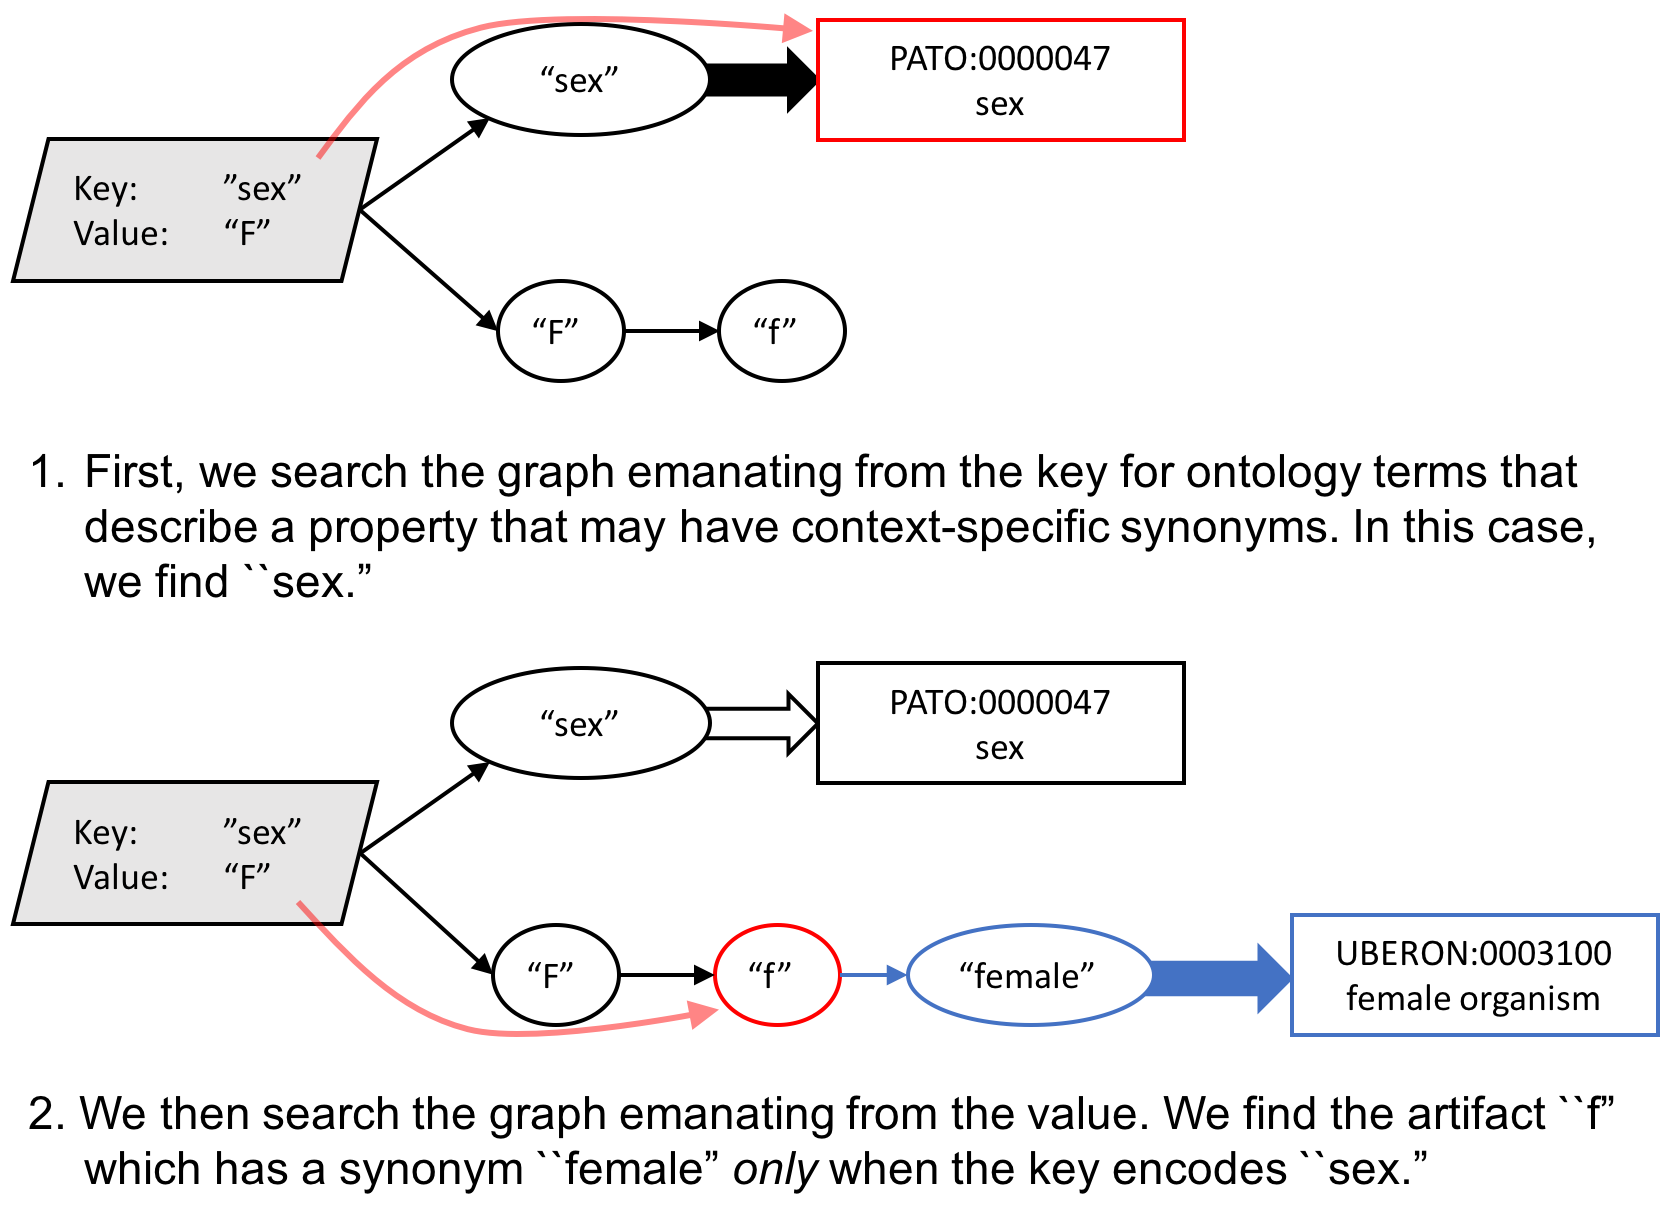
\includegraphics[width=11cm]{figures/context_specific_synonyms.png} 
\caption{\textbf{Extracting context-specific synonyms.} An example describing context specific synonyms.}
\label{fig:context_syn}
\end{figure}

\item \textbf{Fuzzy string matching} We perform fuzzy string matching between the artifacts and the ontology terms.  Let $a$ and $b$ be two strings and let $d(a, b)$ be their Levenshtein edit distance. Let $l(x)$ be the length of a string $x$. An artifact $a$ matches with an ontology term name or synonym $b$ if the following conditions hold: $l(a) > 2$, $d(a,b) \leq 2$, and $d(a,b) \leq \text{max}\{l(a), l(b)\} / 10$. We do not match artifacts that are less than 3 characters long in order to avoid false positive mappings.  If the artifact is greater than 2 characters long, a match is called if the edit distance is less than or equal to 2 and less than or equal to 0.1 times the length of the longer string. For example, the misspelled artifact ``forskin fibroblast'' would match with the ontology term name ``foreskin fibroblast.''  In contrast, the string ``year'' would not match with the ontology term ``ear'' because the edit distance of 1 is greater than 0.1 of the length of the longer string.  When an artifact matches an ontology term, we create a node representing the ontology term and draw an edge from the artifact to the new ontology term node. 

To more efficiently perform fuzzy string matching we store all ontology term names and synonyms in a Burkhard-Keller metric tree \cite{Burkhard} with the bag-distance metric defined in \cite{Bartolini}.  When performing fuzzy string matching between a query string $s$ and the strings in the metric tree, we retrieve all strings in the metric tree that are within a distance of 2 from $s$ using bag-distance. Since bag-distance is a lower-bound on edit-distance, this process filters out all strings in the ontologies whose lower bound on the edit distance is greater than the threshold of 2 that we impose on fuzzy string matching.  We then explicitly compute edit distance between $s$ and the retrieved strings. 

\item \textbf{Matching to custom terms:} There are several noun-phrases that are common in the metadata and that are superstrings of ontology terms, but that do not imply that the sample maps to the contained ontology term.   For example, the phrase ``blood type'' does not imply that the sample was derived from blood.  Similarly, ``tissue bank'' describes the organization that provided the sample, but does not necessarily imply that the sample is a tissue sample. To differentiate the larger noun-phrase from the ontology term it contains, we maintain a custom list of misleading noun-phrases and remove ontology term mappings if those mappings were derived from a substring of a misleading noun-phrase. For example, given the string ``blood type'', the artifact ``blood'' will be blocked from mapping to the ontology term for blood because it is a substring of the noun-phrase ``blood type.'' Currently, we have 27 noun-phrases in our index and we will continue to build this index as we find more misleading noun-phrases that contain ontology terms.


\item \textbf{Remove extraneous cell-line matches:} 
Many cell lines have short names that oftentimes resemble acronyms or gene names.  For example, ``SRF'' is a gene as well as a cell line in the Cellosaurus. Similarly, ``MDS'' is often used as an acronym for Myelodysplastic Syndromes and also happens to be the name of a cell line in the Cellosaurus.

We remove extraneous mappings to cell line terms by searching the graph emanating from the key for a lexical match to ontology terms such as those for ``cell line'' and ``cell type''.  If such a match is \textit{not} found, we search the graph emanating from the value for artifacts that have a lexical match to a cell line ontology term and remove all such ontology term nodes.  This process is illustrated in Figure~\ref{fig:block_cell_line}.

\begin{figure}[htbp]
\centering
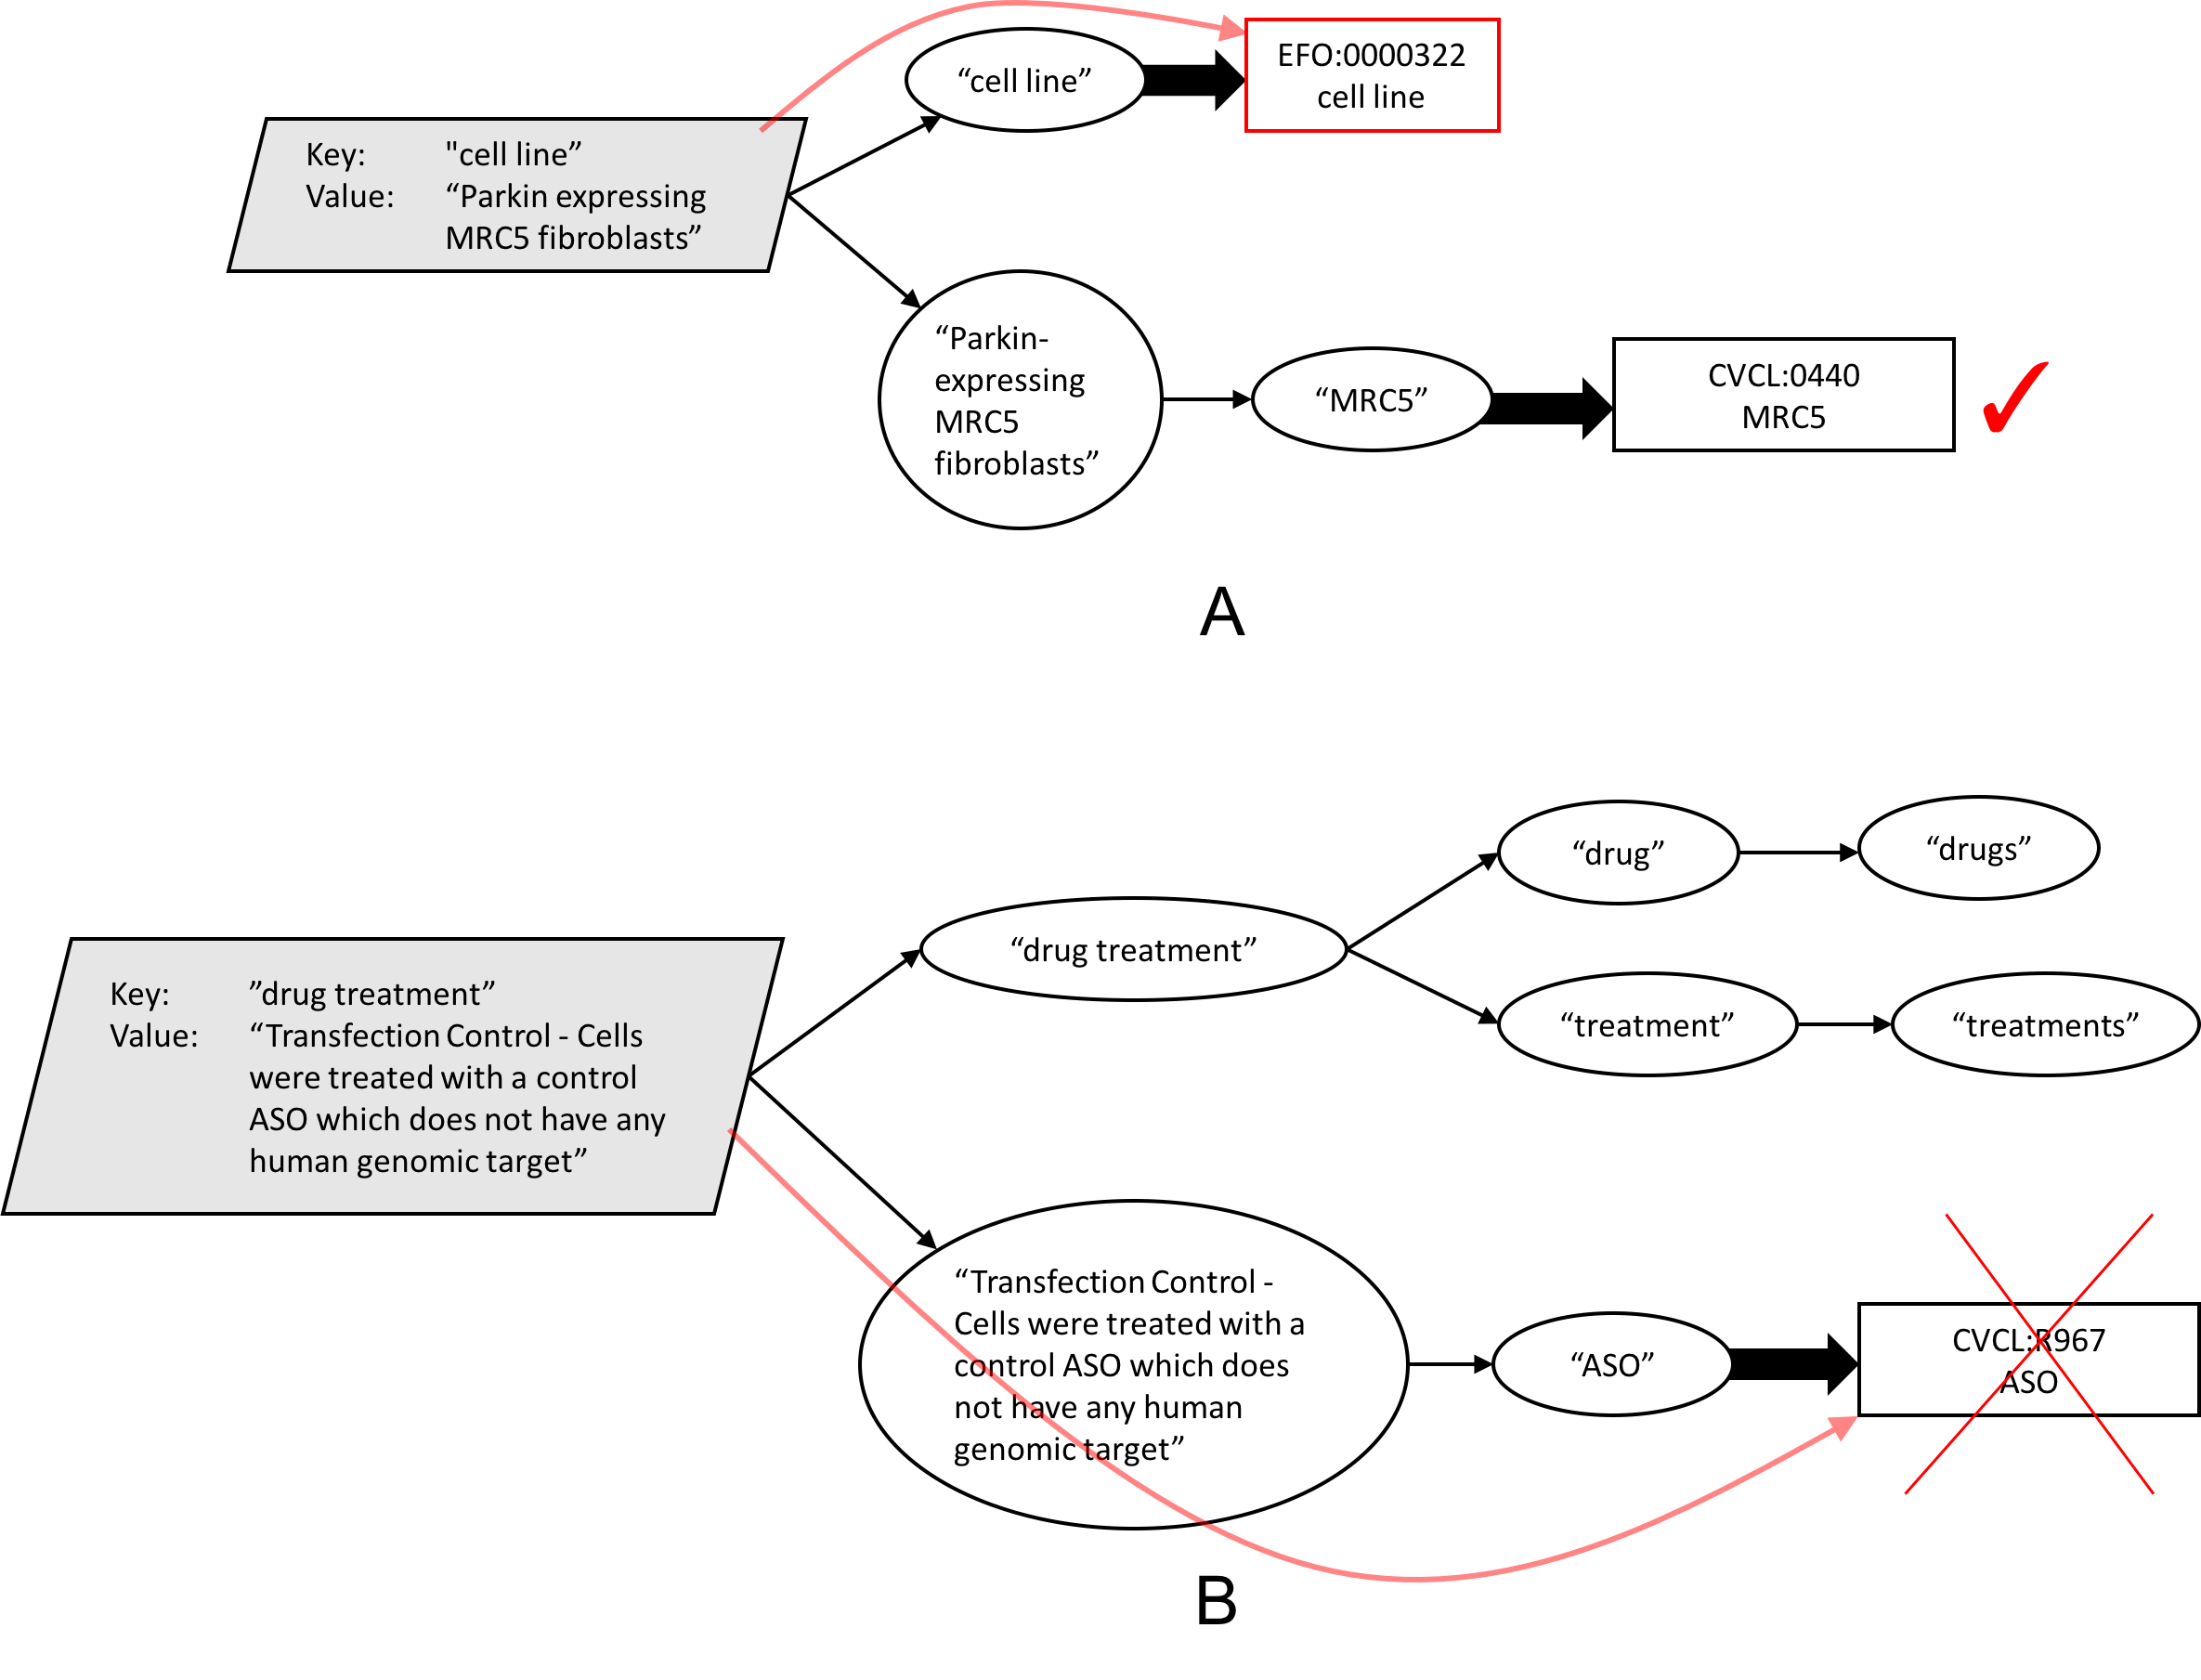
\includegraphics[width=13cm]{figures/block_cell_line.png} 
\caption{\textbf{Removing extraneous cell line terms.} (A) The term ``cell line'' was found in the graph emanating from the key.  Thus, we keep the cell line term for ``MRC5'' in the graph emanating from the value. (B) No ontology term for ``cell line'' or ``cell type'' was found in the graph emanating from the key. We therefore remove the cell line term for ``ASO'' in the graph emanating from the value.}
\label{fig:block_cell_line}
\end{figure}


\item \textbf{Map to linked-superterms:} The domain covered by the EFO overlaps with many of the other ontologies because it includes cell types, anatomical entities, diseases, and cell lines.  In many cases, the EFO is inconsistent with other ontologies in how it draws edges between terms.  For example, the term ``lung adenocarcinoma'' and ``adenocarcinoma'' are present in both the Disease Ontology and the EFO; however ``adenocarcinoma'' is a parent of ``lung adenocarcinoma'' only in the Disease Ontology and not in the EFO.  These inconsistencies pose a problem when we filter for the maximal phrase-length in the metadata.   For example, when a sample maps to ``lung adenocarcinoma'' and ``adenocarcinoma'', we remove ``adenocarcinoma'' because it is a substring of ``lung adenocarcinoma''.  This is valid for the Disease Ontology because the term for ``adenocarcinoma'' is implied by ``lung adenocarcinoma'' by its position in the ontology.  However, this results in a false negative for the EFO version of this term.  

To counteract this problem, we link the terms in the EFO to terms in the other ontologies.  Two terms are linked when they share the same term-name or exact-synonym.  Then, when an artifact maps to a term, we traverse the term's ancestors and map to any terms that are linked to those ancestors.   In the case of ``lung adenocarcinoma'', we would traverse the ancestors of this term in the Disease Ontology and map to the EFO's ``adenocarcinoma'' because it is linked to the Disease Ontology version of this term. Figure~\ref{fig:linked} illustrates this process. 


\item \textbf{Cell line disease implications:} The EFO is missing edges between disease cell line terms and the corresponding disease terms. For example, the term ``cancer cell line'' does not have an edge to ``cancer.''  To fill this gap, if a sample maps to a cell line category term, we also map to the corresponding disease terms. 


\item \textbf{Block superterm mapping:} It is a common occurrence for disease ontology terms to include anatomical entities in their name. For example, ``breast cancer'' includes ``breast'' as a substring. It would be incorrect to map ``breast'' to the sample because this word localizes the cancer, but does not localize the origin of the sample.  We note that it is possible that the sample was indeed derived from breast tissue; however, it is also possible the sample originated from other tissue such as a malignant site.  We maintain a conservative approach and avoid mapping to ``breast.''  We implement this process by designing each artifact node to keep track of the original character indices in the metadata from which it was derived. After mapping all artifacts to the ontologies, we remove all ontology terms that were lexically matched with an artifact node that is subsumed by another artifact node that matches with another ontology term.  

\item \textbf{Custom consequent mappings:}  We maintain a small list of 6 common terms that imply other terms.  For example, if a cell maps to a the EFO term for ``cell line'', we consequently map the sample to the Cell Ontology's term for ``cultured cell.''  

\item \textbf{Real-value property extraction:} We maintain a list of ontology terms that define real-value properties. Currently, we use 6 terms: ``age'', ``passage number'', ``timepoint'', ``age at diagnosis", ``body mass index", and ``age at death."  Future work will entail expanding this list.  To extract a real-value property from a key-value pair, we search the graph emanating from the key for a match to a property ontology term.  If such a property is found, we search the graph emanating from the value for an artifact representing a numerical value and a unit ontology term node (e.g., ``46'' and ``year'').  From this process, we extract the triple (property, value, unit). For example, given the key-value pair \texttt{age: 46 years old}, we extract (``age'', 46, ``year'').


\item \textbf{Filtering mapped ontology terms by semantic similarity:}
The ontologies are structured so that each synonym of an ontology term is given a synonym-type. These types include ``exact'', ``broad'', and ``narrow.'' These synonym-types describe the relationship between the synonym string and the term name.  An ``exact'' synonym indicates that the string is semantically closer to the ontology term name than a ``broad'' synonym.  If an artifact matches to multiple ontology terms, the ontology term with the semantically nearest matched target is likely to be the best match with the artifact. Thus, given an artifact with multiple matched terms, we examine the targets within the matched terms to which the artifact matched and rank these targets according to the semantic similarity with the ontology term name.  We then keep the match with the highest similarity and discard the rest.  

For example, given the artifact ``skin'', we find several terms in the Uberon ontology that have a synonym ``skin'':  ``zone of skin'' (exact synonym), ``skin epidermis'' (broad synonym), ``skin of body'' (related synonym), and ``integument'' (related synonym). Of these terms, ``skin'' is semantically most similar to the term ``zone of skin'' because it is an exact synonym of this term.  We therefore keep this mapping and discard the rest.

\item \textbf{Consequent cell line mappings:} Our pipeline draws edges between cell line ontology term nodes and the ontology terms that describe the cell line.   For example, if the TRG contains the node for the cell line ``HeLa'', we draw an edge to the ontology terms for ``adenocarcinoma'' and ``female'' because this cell line was derived from a woman with cervical adenocarcinoma.  We consider such mappings to be consequent mappings because they are retrieved using an external knowledge base.   
 
 This knowledge base was created from data we scraped from the ATCC website at \url{https://www.atcc.org}. To construct mappings between cell lines and ontology terms, we ran a variant of our pipeline on the scraped cell line data.  We scraped cell line metadata for all cell lines that are present in the Cellosaurus. 

\item \textbf{Consequent developmental stage mappings:} If the sample maps to a real-value property with property ``age'' and unit ``year'', we check whether the value is greater than 18. If so, we consequently map the sample to the EFO and Uberon terms for ``adult.''
\end{enumerate}


\section{Detailed description of sample-type prediction procedure } \label{sec:sample_pred}

Although we train a one-vs-rest classifier using logistic regression binary classifiers, we ultimately use a custom decision procedure for making a sample-type prediction.  This procedure entails limiting the possible predicted sample-types based on ontology terms that were mapped by our computational pipeline.  The algorithm chooses among the remaining possible sample-types by selecting the sample-type with highest confidence according to the one-vs-rest classifier.    

To provide an example, if the ontology term ``stem cell'' was mapped to the sample, we set $p(y = j | x) = 0$ for $j \in \{\text{\texttt{ tissue, cell line, primary cells}}\}$.  We then compute the probabilities $p_i := \frac{p(y=i \mid x)}{\sum_h p(y = h \mid x)}$ for each $i$.  Our final prediction is then $\hat{y} = \text{argmax}_i p_i$. In summary, this process asserts that if ``stem cell'' mapped to the sample, then the sample must be either a stem cell sample, in vitro differentiated cell sample, or induced pluripotent stem cell sample. We let the classifier decide which is the most likely label among these possible labels. 

More specifically, we follow the following steps for making a prediction:
\begin{enumerate}
\item If the sample maps to ``xenograft'' (EFO:0003942), then we predict \texttt{ tissue} with confidence 1.0.
\item If the sample was passaged (i.e. maps to a real-value property tuple with property ``passage number'' and unit ``count''), then we assert the sample cannot be \texttt{ tissue}. If the number of passages is greater than 0, then we assert the sample cannot be \texttt{ primary cell}.
\item If the sample maps to a cell line, then we check the Cellosaurus for the cell line category.  We map the Cellosaurus cell-line category to a set of possible sample types as follows:
\begin{itemize}
    \item Induced\_pluripotent\_stem\_cell: \texttt{ in vitro differentiated cells}, \texttt{ induced pluripotent stem cell line}
    \item Cancer\_cell\_line: \texttt{ cell line}
    \item Transformed\_cell\_line: \texttt{ cell line}
    \item Finite\_cell\_line: \texttt{ cell line}
    \item Spontaneously\_cell\_line: \texttt{ cell line}
    \item Embryonic\_stem\_cell: \texttt{ stem cells}, \texttt{ in vitro differentiated cells}
    \item Telomerase\_cell\_line: \texttt{ cell line}
    \item Conditionally\_cell\_line: \texttt{ cell line}
    \item Hybridoma: \texttt{ cell line}
\end{itemize}
\item If the sample maps to the term ``stem cell'', then we remove the possibility that the sample type is \texttt{ cell line}, \texttt{ tissue}, or \texttt{ primary cells}.  
\item If the sample maps to a specific cell-type term (i.e. any term that is a child of ``somatic cell''), then we remove the possibility that the sample-type is \texttt{ tissue}. This follows from our observation that when the metadata describes a specific cell-type, the sample consists of homogenous cells that have been isolated and filtered.  The sample no longer consists of cells positioned in their original three dimensional structure and is thus not a tissue sample.
\end{enumerate}







\chapter{MetaSRA web interface } \label{app:website}

We developed a web interface website to enable querying the RNA-seq data in the SRA using the MetaSRA-mapped ontology terms, thereby facilitating discovery of public RNA-seq data. Matt Ziegler was the lead developer; however, I worked alongside Matt in designing the interface to the website and performing user-interviews to assess usability.   The website presents a number of features that take advantage of the MetaSRA schema discussed in Chapter~\ref{chap:2}:

\begin{itemize}
\item \textbf{Boolean queries:} We enable basic Boolean queries in which the user can specify a set of terms that the user requires for all search results as well as a set of terms that are used to filter search results (Fig~\ref{fig:webpage}).  Further, the user is able to filter their search results according to the MetaSRA's predicted sample-type category.
\begin{figure}[htbp]
\centering
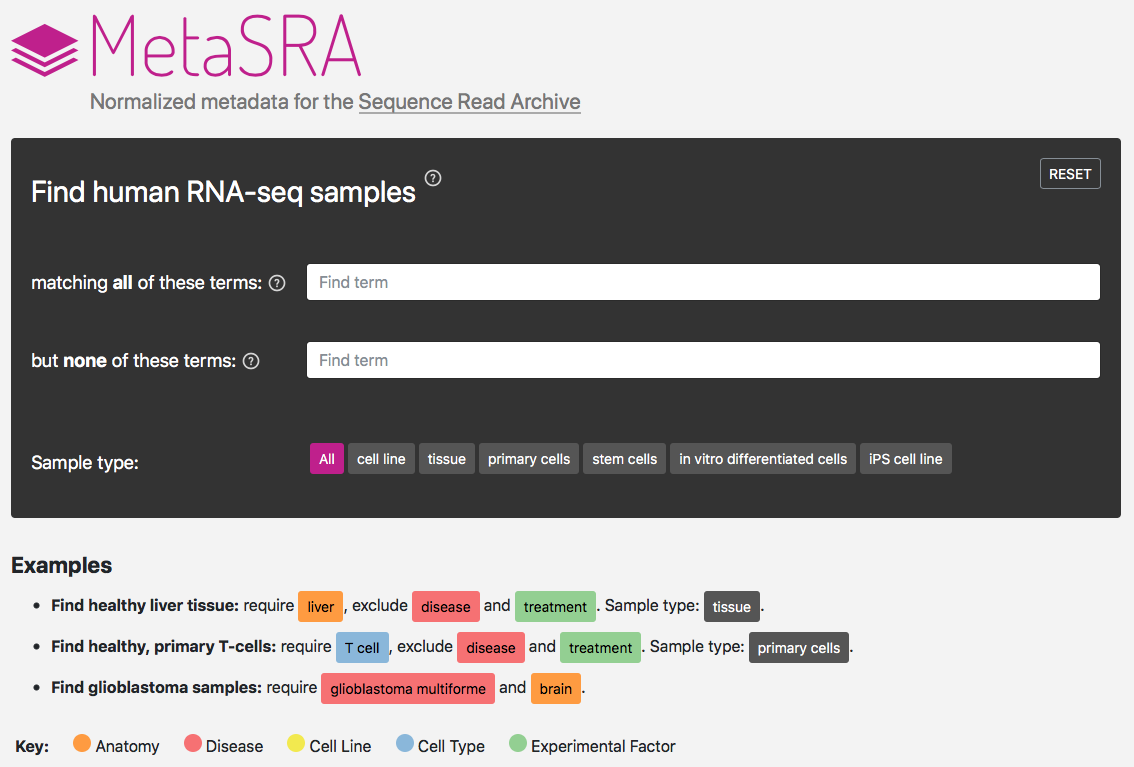
\includegraphics[width=12cm]{figures/web_page.png}  
\caption{\textbf{MetaSRA homepage.} A screenshot of the homepage for the MetaSRA website.}
\label{fig:webpage}
\end{figure}

\item \textbf{Ontology-based autocomplete}: The website requires that the user queries the metadata using ontology terms; however, this design-choice requires that users know what terms exist in the ontology \textit{a priori}.  This is often an unreasonable expectation of users. Therefore, we implemented an autocomplete feature (also called ``search suggestions") in order to help the user formulate their query using valid ontology terms. As the user is typing a query, a drop down menu appears with suggested ontology terms that may match the concept that the user has in mind.  Furthermore, each of these search-suggestions also presents ancestral terms (i.e. more general terms) and descendent terms (i.e. more specific terms) in order to further help the user discover queryable terms  (Fig.~\ref{fig:autocomplete}).  
\begin{figure}[htbp]
\centering
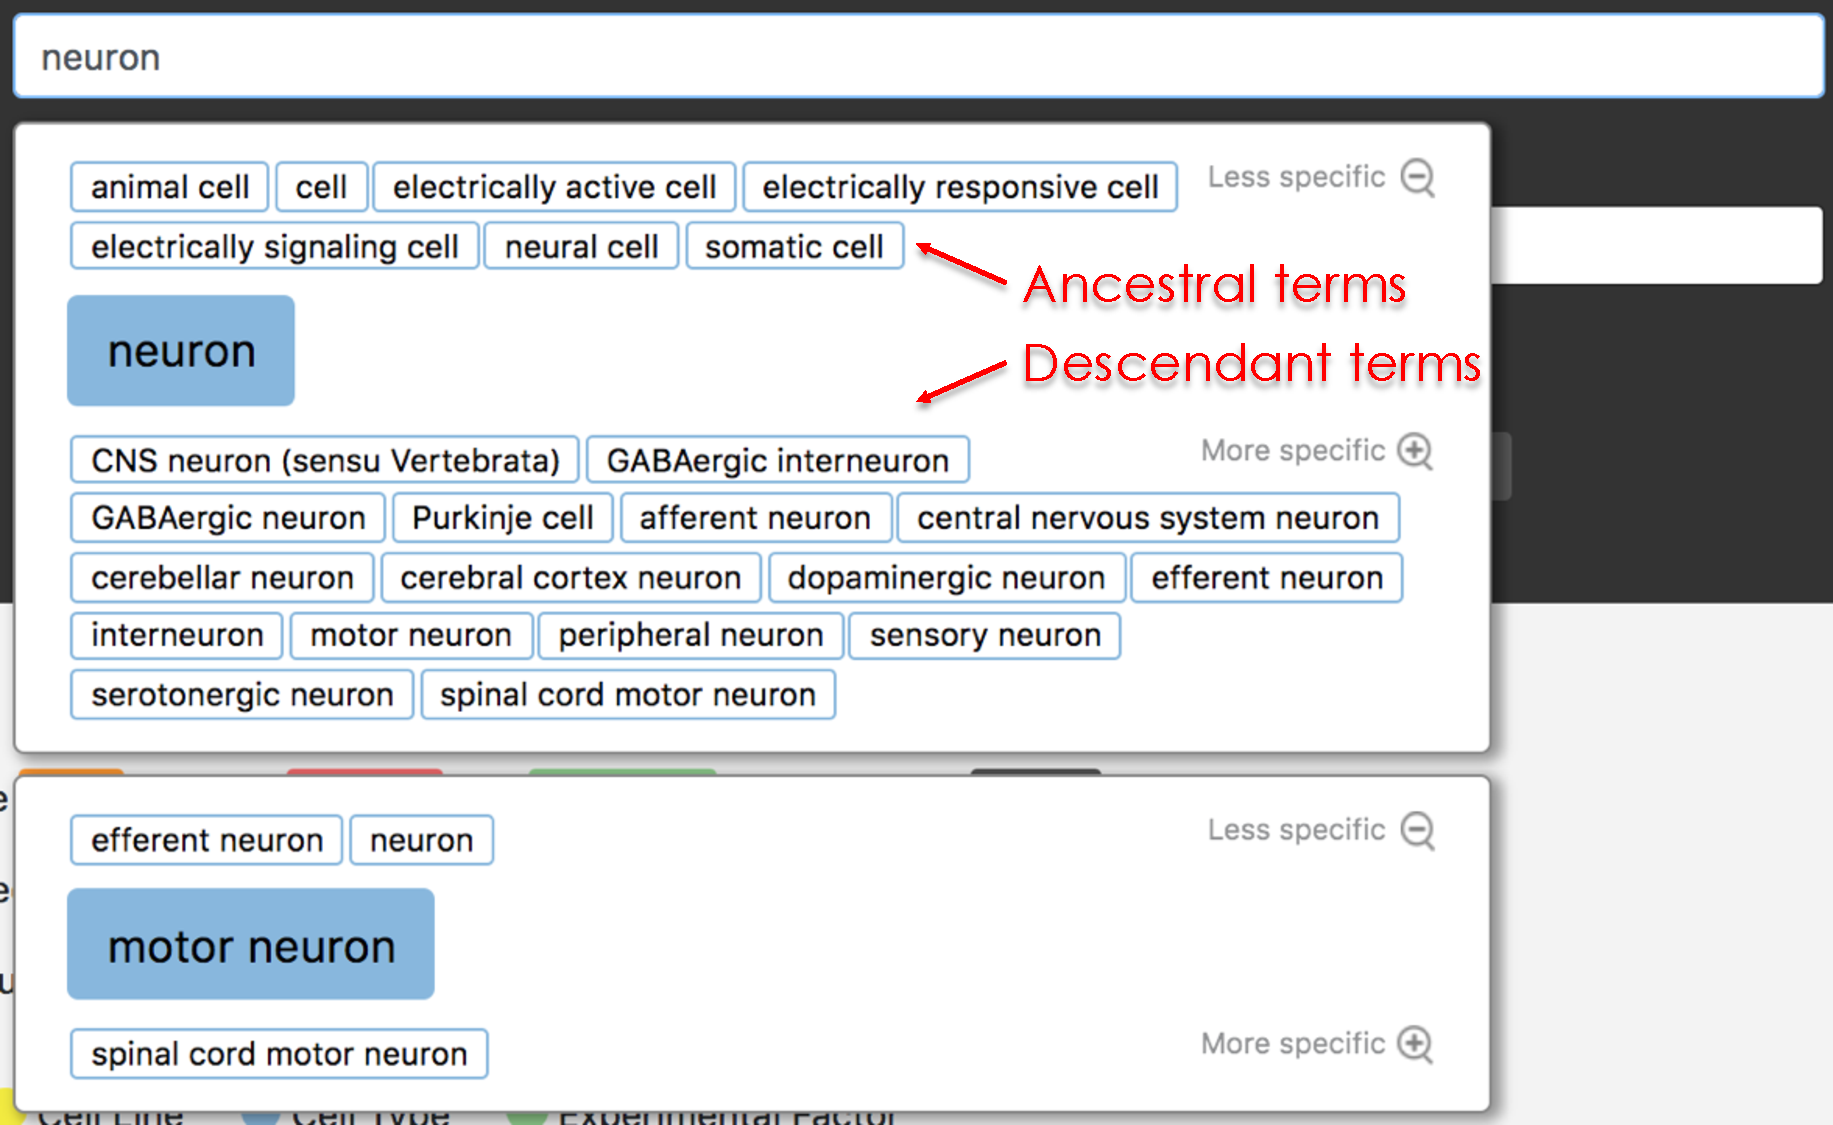
\includegraphics[width=12cm]{figures/autocomplete.pdf}  
\caption{\textbf{Autocomplete.} A screenshot of the autocomplete, search-suggestions that appear when the user types the query ``neuron".}
\label{fig:autocomplete}
\end{figure}

\item \textbf{Sample-set summaries:} We group the search-results by samples that all share identical metadata (and thus, also share identical mapped ontology terms) (Fig.~\ref{fig:search_results}).  This format avoids overwhelming the user with redundant search results. 
\begin{figure}[htbp]
\centering
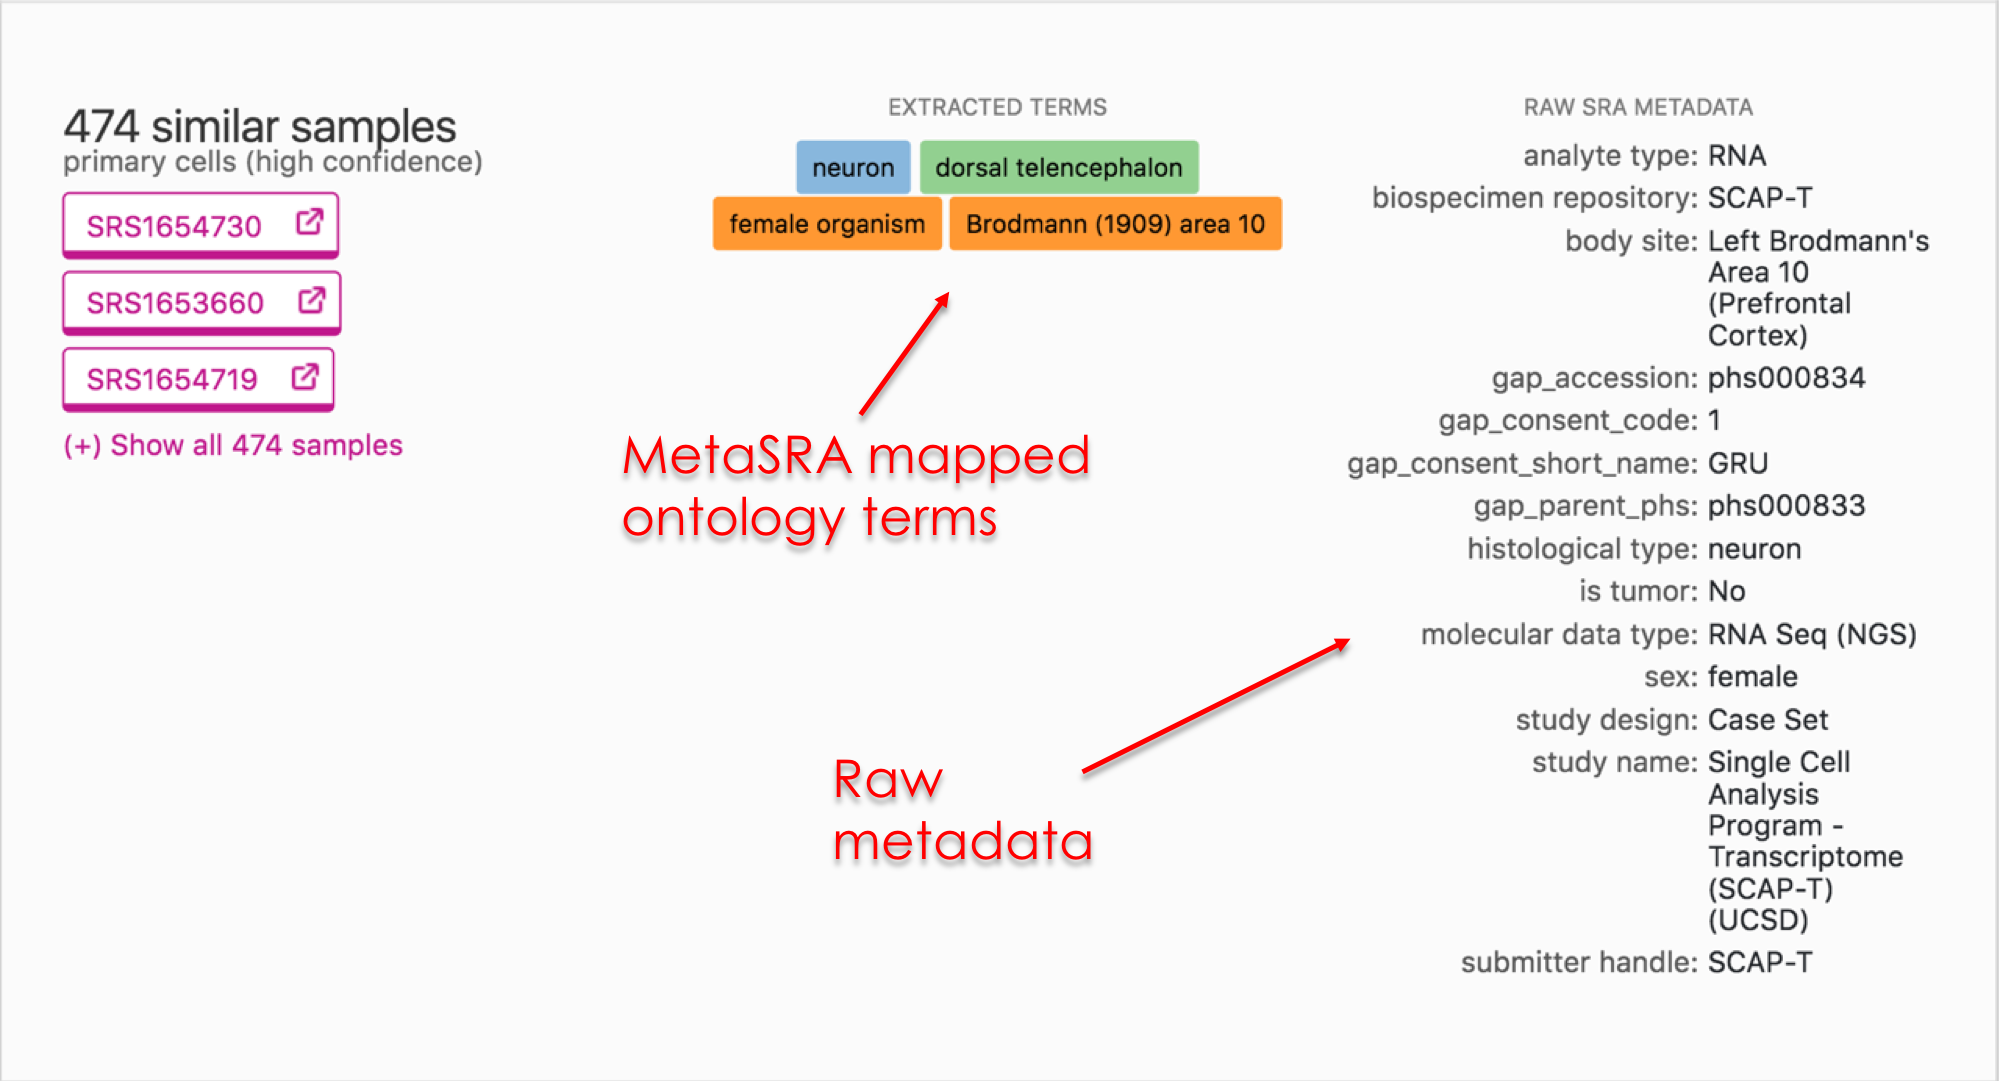
\includegraphics[width=12cm]{figures/search_results.png}
\caption{\textbf{Search results.} A screenshot of a set of samples returned by the query "neuron". These samples all share the same metadata and therefore are grouped into a single entry.  For each such group, we display the mapped ontology terms along with the original, raw metadata.}
\label{fig:search_results}
\end{figure}


\item \textbf{Search result term-clouds:} An important concern that users may have when querying the public data are co-occurring terms/phenotypes of the search results. For example, a user who is querying for samples from patients with diabetes, may wish to know about other characteristics of the search results such their cell type or tissue of origin.  To summarize this information, we present a ``term-cloud" of all terms that frequently co-occur with the search results (Fig.~\ref{fig:term_cloud}). Furthermore, the user can use the term cloud to further refine their search by selecting terms to further filter their results. 

\begin{figure}[htbp]
\centering
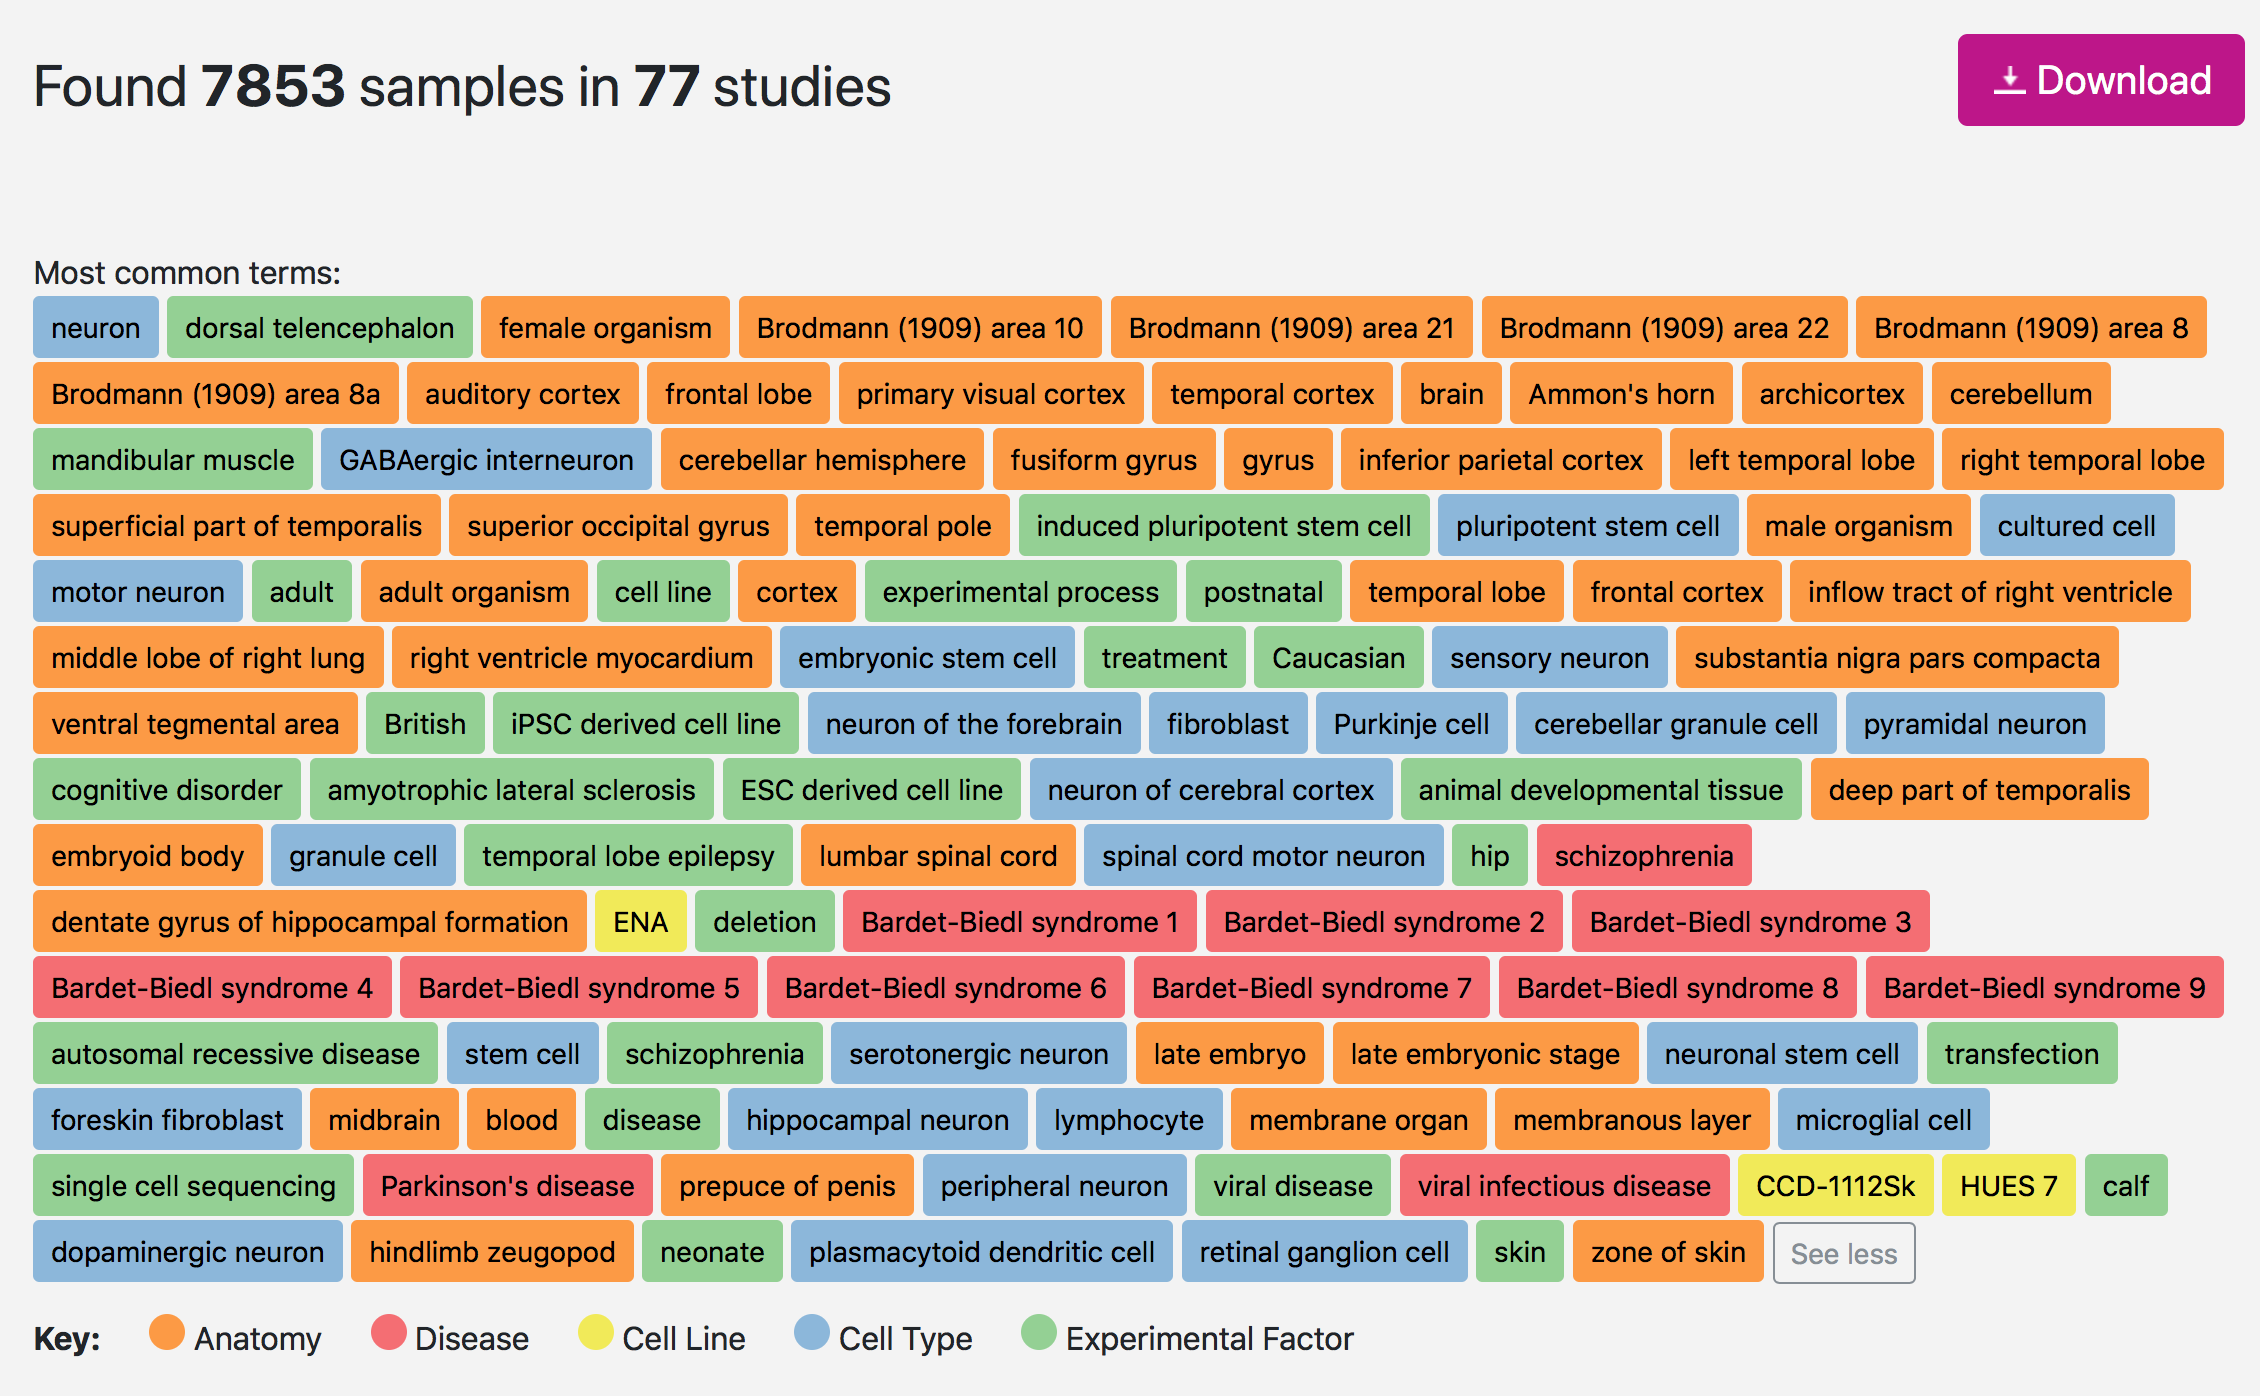
\includegraphics[width=12cm]{figures/term_cloud.png}
\caption{\textbf{Term cloud.} A screenshot of a the search results term cloud for the query "neuron".}
\label{fig:term_cloud}
\end{figure}

\end{itemize}






\chapter{Detailed description of experiment evaluating effects of training on heterogeneous data } \label{app:sample_pred}

\section{Description of experiment }

To test the effects of data heterogeneity in training, we performed an experiment that involved training a set of binary classifiers using both homogeneous training sets, where the positive examples all originate from the same study, and heterogeneous datasets, where positive examples originate from multiple studies.  First, the notation we will use to describe these experiments is as follows: Let
\begin{align*}
X &:= \text{the set of all samples in the data set}\\
S &:= \text{the set of studies with at least with at least one sample in $X$}
\end{align*}
For a given cell type $c$, let
\begin{align*}
X_c \subset X &:= \text{the set of  all samples of cell type }c\\
X_{\neg c} &:= X \setminus X_c
\end{align*}
Given a set of samples $A \subseteq X$, we define the function 
$$T(A) := \text{the set of all studies with at least one sample in $A$}$$ 
Given a study $s \in S$, let
\begin{align*}
X_{c,s} \subset X_c &:= \text{the subset of $X_c$ from study $s$} \\
X_{\neg c,s} \subset X_{\neg c} &:= \text{the subset of $X_{\neg c}$ from study $s$}
\end{align*}


The experiment proceeds as follows: for a given cell type $c$, we perform a cross-validation-like scheme where for each study $s_{\text{test}} \in T(X_c)$, we create a set of held out test samples. The positive test samples come from study $s_{\text{test}}$. That is, 
$$\text{Test\_Pos}_{c,s_{\text{test}}} := X_{c,s_{\text{test}}}$$ 
The negative test items are subsampled from all studies that have no samples of cell type $c$. That is, 
$$\text{Test\_Neg}_{c,s_{\text{test}}} \subset \text{The union of samples from studies not in $T(X_c)$}$$ 
%X_{\neg c} \setminus \left(\bigcup_{s \in T(X_{c})} X_{\neg c, s}\right)$$
This ensures that the training and test samples are divided along study boundaries.  The test set for cell type $c$ and held-out study $s$ is then constructed as
$$\text{Test}_{c,s_{\text{test}}} := \text{Test\_Pos}_{c,s_{\text{test}}} \cup \text{Test\_Neg}_{c,s_{\text{test}}}$$
Every homogeneous training set and heterogeneous training set, will contain an identical set of negative training items that are sub-sampled from all studies that do not have data in the test set.  That is,
$$\text{Train\_Neg}_{c,s_{\text{test}}} \subset \left\{x \in X_{\neg c} \ : \ \text{$x$ is not from a study in the test set} \right\}$$
We want to ensure that all training sets have an identical number of examples. Since they all share the same negative examples, we must ensure that all training sets also have the same number of positive examples. To ensure this, we compute the minimum sized set of positive examples coming from a single held-in study:
$$k := \text{min} \ \{|X_{c,s}| : s \in T(X_c) \setminus \{s_{\text{test}}\}\}$$
Now, we create sets of homogeneous positive examples as follows: for each held-in study $s_{\text{train}} \in S_c \setminus \{s_{\text{test}}\}$, we create $L$ homogeneous training sets. That is, for each $l \in [L]$, the $l$th training set's positive examples consist of $k$ random samples from $T(X_{c, s_{\text{train}}})$. That is,
$$\text{Homog\_Train\_Pos}_{c,s_{\text{test}},s_{\text{train}},l} \subset X_{c,s_{\text{train}}}$$
where 
$$|\text{Homog\_Train\_Pos}_{c,s_{\text{test}},s_{\text{train}},l}| = k$$
Each homogeneous training set is then constructed as 
$$\text{Homog\_Train}_{c,s_{\text{test}},s_{\text{train}},l} := \text{Homog\_Train\_Pos}_{c,s_{\text{test}},s_{\text{train}},l} \cup \text{Train\_Neg}_{c,s_{\text{test}}}$$
Thus, for each cell type $c$, for each held-out study $s_{\text{test}}$, we construct $L \times |T(X_c) - 1|$ homogeneous training sets. That is, they each contain positive examples coming from a single study.

For each cell type $c$ and held out study $s_{\text{test}}$, we create $L$ heterogeneous training sets for which the positive examples are sub-sampled from all of the held-in studies. That is, for each held-in study $s_{\text{train}} \in T(X_c) \setminus \{s_{\text{test}}\}$, we sub-sample $k / |T(X_c) - 1|$ samples and add them to the heterogeneous training set giving us 
$$\text{Heter\_Train\_Pos}_{c,s_{\text{test}},l} \subset X_c$$
where 
$$|\text{Heter\_Train\_Pos}_{c,s_{\text{test}},l}| = k$$

For each cell type $c$ and held out study $s_{\text{test}} \in T(X_c)$, we train a classifier on all of the homogeneous training sets and heterogeneous training sets and evaluate on the test set $\text{Test}_{c,s_{\text{test}}}$. We compute the average-precision (AP) score for each classifier.  Thus, for each held-in study $s_{\text{train}} \in T(X_c) \setminus \{s_{\text{test}}\}$, we have $L$ average-precision scores corresponding to the homogeneously trained classifiers for that study.
We denote the average-precision score from each homogeneously trained classifier as $\text{Homog\_Avg\_Prec}_{c,s_{\text{test}},s_{\text{train}},l}$.  We also have $L$ average-precision scores for the heterogeneously trained classifiers. We denote the average-precision score for each classifier as $\text{Heter\_Avg\_Prec}_{c,s_{\text{test}},l}$.

\section{Analysis }

We compare the performance of the homogeneously trained classifiers versus the heterogeneously trained classifiers using two strategies. First, for each held out study $s_{\text{test}}$, we compute the mean average-precision (MAP) over \textit{all} homogeneously trained classifiers:
$$\text{Homog\_MAP}_{c,s_{\text{test}}} := \frac{1}{L|T(X_c)-1|} \sum_{s_{\text{train}} \in T(X_c) \setminus \{s_{\text{test}}\}} \sum_{l=1}^L \text{Homog\_Avg\_Prec}_{c,s_{\text{test}},s_{\text{train}},l}$$
The corresponding mean-average precision for the heterogeneously trained classifiers are defined as
$$\text{Heter\_MAP}_{c,s_{\text{test}}} := \frac{1}{L} \sum_{l=1}^L \text{Homog\_Avg\_Prec}_{c,s_{\text{test}},s_{\text{train}},l}$$
Figure~\ref{fig:homo_vs_hetero_setup} displays a scatter plot that plots each 
$$(\text{Homog\_MAP}_{c,s_{\text{test}}}, \text{Heter\_MAP}_{c,s_{\text{test}}})$$ 
pair where each point is colored by $c$. This analysis shows that, on average, a classifier trained on data from multiple studies, will outperform a classifier trained on data from only on study.
\chapter{Implementation of Bayesian Network Correction } \label{app:bnc}

We implemented the URSA algorithm described by \cite{Lee2013}.  Before we proceed, we introduce the notation used in this Appendix for describing our implementation:
\begin{itemize}
\item $i := $ the index of a label
\item $Y_i := $ a latent random variable corresponding to whether to assign label $i$ to the sample
\item $\tilde{Y}_i := $ random variable corresponding to the distribution over classifier scores for label $i$ 
\item $\bold{P}_i := $ set of parent of $Y_i$
\item  $\bold{C}_i := $ set of children random variables of $Y_i$ that are also latent random variables. That is, all children of $Y_i$ except for $\tilde{Y}_i$
\item  $\bold{S}_i := $ set of all parents of all random variables in the set $\bold{C}_i$ except for $Y_i$
\item $\bold{A}_i := $ set of all ancestors of $Y_i$
\end{itemize}
We note that bold random variables highlight the fact that the random variable is a set of random variables. We let the lowercase version of these random variables denote the value for a realization of the corresponding random variable (e.g. $X = x$). We also let $p(x)$ be shorthand for $p(X = x)$, the probability (if $X$ is discrete) or density (if $X$ is continuous) that random variable $X$ equals $x$. 


\section{Estimation of classifier output distributions }

For a given cell type $i$, we estimate the conditional distribution of the classifier's output $\hat{y}_i$ (distance to the decision boundary) conditional on its true label $y_i$ as a discrete random variable constructed by binning the classifier outputs  $\hat{y}_i$ as output in a 2-fold cross-validation process. Specifically, we partition the training data for cell type $i$ into two folds ensuring that no study is split between folds while attempting to keep the sizes of the two folds as similar as possible. We then train on one fold and compute the classifier scores from the second fold (for each of the two folds).

Using all of these scores, we then estimate a histogram using a second 2-fold cross-validation scheme. We compute the width of the histogram using the range of scores. We then test a number of bin sizes by first estimating a histogram density function using data in one fold and then computing the likelihood of the data in the second fold (performing this procedure for both folds). The histogram density function is given by
$$f(x) := \frac{1}{nh}\text{Count}(x) $$
where $n$ is the total number of data points, $h$ is the width of each bin, and $\text{Count}(x)$ is the number of data points sharing the same bin as $x$. 
We choose a bin size that maximizes the mean of the two data log likelihoods computed on each fold.


\section{Estimation of the prior distribution }

As described by Lee \textit{et al.} (2013), the true cell type assignments $p(y_1, \dots, y_n)$ factor according to the ontology graph:
$$p(y_1, \dots, y_n) := \prod_{i=1}^m p(y_i \mid \bold{c}_i)$$
These conditional distributions $p(y_i \mid \bold{c}_i)$ enforce consistency with the ontology:
 $$p(Y_i=1 \mid \bold{c}_i) := \left\{
     \begin{array}{lr}
       1.0 & : 1 \in \bold{c}_i   \\
       \text{prior}_i & : \text{otherwise}
     \end{array}
     \right.$$
The $\text{prior}_i$ values are computed from counts in the training data. Specifically, the prior for each leaf-node cell type $\ell$ is simply the fraction of samples in the data set labelled as $\ell$.  For each internal node $\ell$, the prior is computed as the fraction of all samples  labelled as $\ell$, but not labelled as any child of $\ell$. A pseudocount of one was used in the calculation for all priors.

\section{Gibbs sampling algorithm }

Gibbs sampling is a member of a family of techniques, called Markov chain Monte Carlo (MCMC), for sampling from a complex joint probability distribution. Given a joint distribution over a set of random variables $P(\bold{X})$ where $\bold{X} := \{X_1, \dots, X_n\}$, Gibbs sampling involves first initializing all of the random variables to some preset values and then iteratively sampling each random variable from its distribution conditioned on the current values of the remaining random variables (Algorithm~\ref{algo:gibbs}). As the number of iterations approaches infinity, the samples from this procedure will approach the target joint distribution. Of course, in practice, only a finite number of samples can be obtained; however, with sufficient numbers of samples, an approximate estimate can be obtained. Usually, some number of initial samples are discarded in order for the Markov chain to approach its stationary distribution, at which point, the sampling distribution will more closely resemble the target distribution. In order to implement Gibbs sampling, one must be able to sample from each random variable conditioned on the remaining random variables.

\begin{algorithm}
\caption{Gibbs Sampling}
\label{algo:gibbs}
\begin{algorithmic}
\State $t \gets 0$
\For{$i = 1, \dots, n$}
	\State $x_i^{(t)} \gets \text{Some, possibly random, initial and valid value for } X_i$
\EndFor
\For{$t = 1, \dots, T$}
	\For {$i = 1, \dots, n$} 
		\State $x_i^{(t)} := x_i^{(t-1)}$
	\EndFor
	\For {$i = 1, \dots, n$}
		\State $x_i^{(t)} \sim p(x_i \mid \bold{x}^{(t)} \setminus x_i^{(t)})$
	\EndFor
\EndFor
\end{algorithmic}
\end{algorithm}

In Bayesian networks, each random variable's Markov blanket consists of its parents, its children, and it's children's parents. In the Bayesian network for BNC, each conditional distribution can therefore be computed using:
\begin{align*}
p(y_i \mid \tilde{y}_i, \bold{s}_i, \bold{c}_i, \bold{p}_i) &\propto p(y_i, \tilde{y_i}, \bold{s_i}, \bold{c}_i, \bold{p_i}) \\
&= p(\tilde{y}_i \mid y_i) p(y_i \mid \bold{p}_i) p(\bold{c}_i \mid y_i, \bold{s}_i)  \\
&= p(\tilde{y}_i \mid y_i) p(y_i \mid  \bold{p}_i)  \prod_{y_j \in \bold{c}_i} p(y_j \mid y_i, \bold{p}_j \setminus y_i)\\
&=  \left\{
     \begin{array}{lr}
       p(\tilde{y}_i \mid y_i) p(y_i \mid  \bold{p}_i)  \prod_{y_j \in \bold{c}_i} p(y_j \mid y_i, \bold{p}_j \setminus y_i)  : y_i = 1  \\
       p(\tilde{y}_i \mid y_i) p(y_i \mid  \bold{p}_i)  \ \ \ \ \ \ \ \ \ \ \ \ \ \ \ \ \ \ \ \ \ \ \ \ \ \ \ \ \ \  \ \ \ \ \ \ \ \ \ \ \ \ : y_i = 0
     \end{array}
   \right.
\end{align*}
where the normalizing constant is
$$Z := \left[\sum_{y_i \in \{0,1\}} p(\tilde{y}_i \mid y_i) p(y_i \mid  \bold{p}_i) \prod_{y_j \in \bold{c}_i} p(y_j \mid y_i, \bold{p}_j \setminus y_i) \right]^{-1}$$


The construction of the Bayesian network in BNC admits a fast Gibbs sampling algorithm.  This algorithm relies on the observation that if, during the course of Gibbs sampling, a given node has any parent that is assigned (i.e. equal to one), then this node will also be assigned with probability one. Therefore, there is no need to explicitly sample this node. Similarly, if a node has any child that is unassigned (i.e. equal to zero), then this node will also be unassigned with probability one.  This observation leads to a sped up Gibbs sampling algorithm that avoids sampling every random variable on each iteration (Algorithm~\ref{algo:gibbs_bnc}).  In this algorithm, the nodes are visited according to the topological order of the DAG and a set is maintained that keeps track of those nodes that do not need to be explicitly sampled on their next visit.  When a node changes its assignment value (from zero to one, or one to zero), the set of skippable nodes is updated (Fig.~\ref{fig:gibbs_bnc}).

\begin{figure*}[!tpb]
\centerline{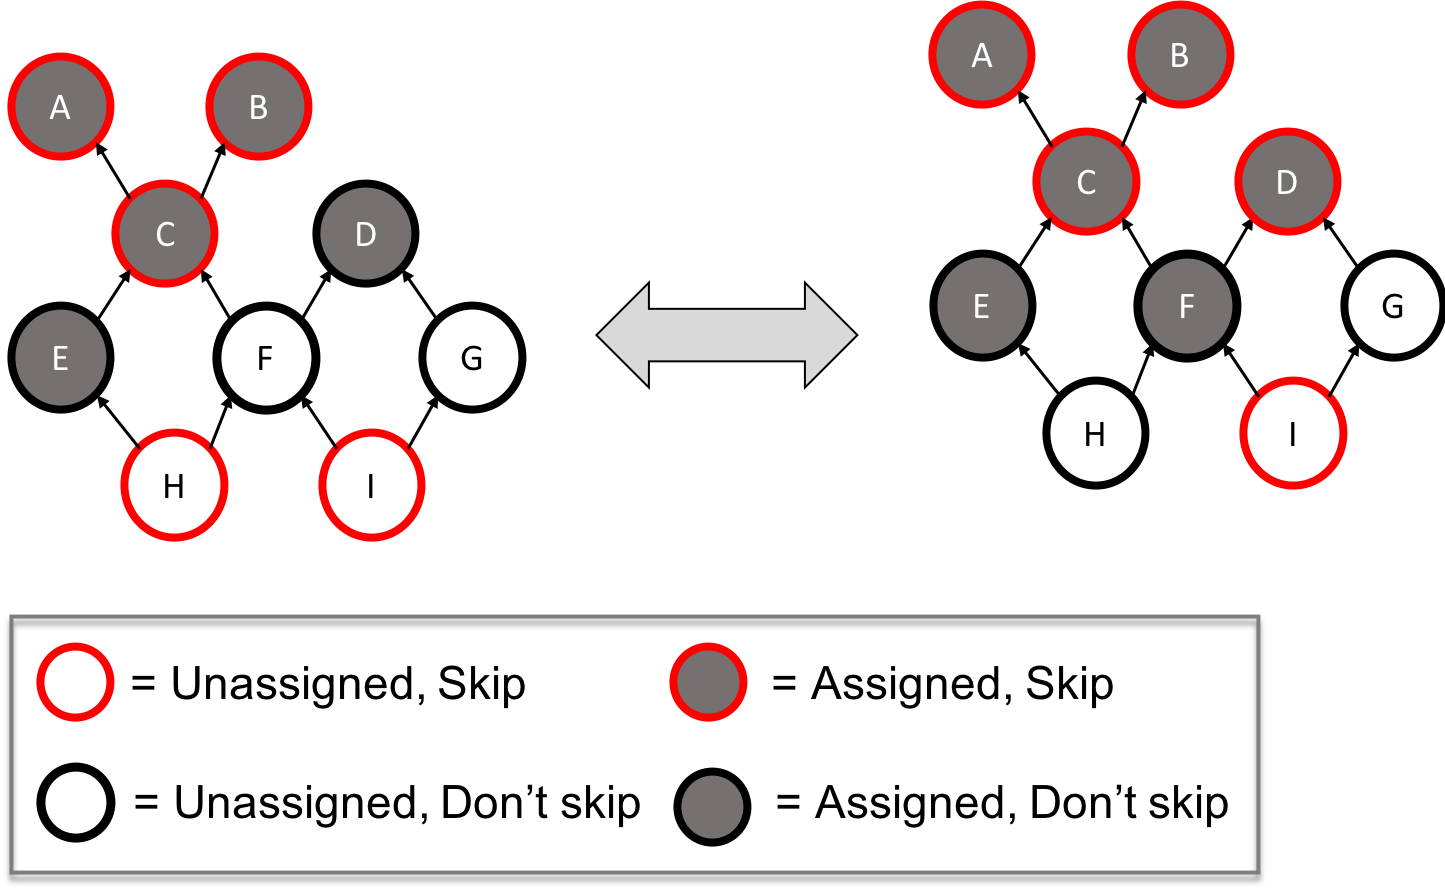
\includegraphics[width=11cm]{figures/gibbs_bnc.png}}
\caption{\textbf{Gibbs sampling for BNC.} An example depicting a step in the BNC Gibbs sampling algorithm. The node labelled "F" has either switched from unassigned to assigned (left-to-right) or from assigned to unassigned (right-to-left). Upon switching its assignment, the algorithm updates the set of nodes for which sampling does not need to be performed explicitly upon their next visit (nodes circled red).}
\label{fig:gibbs_bnc}
\end{figure*}

\begin{algorithm}
\caption{Gibbs Sampling for Bayesian Network Correction}
\label{algo:gibbs_bnc}
\begin{algorithmic}
\Procedure{GibbsForBNC}{$L, T$} \Comment{$L$ is the set of latent variable nodes in the DAG. $T$ is the number of iterations to run Gibbs sampling.}
\State $\text{Skip} \gets \emptyset$ \Comment{The set of random variables that don't require sampling}
\State $\bold{y}^{(0)} \gets \Call{Initialize}{L}$ \Comment{Initialize the random variables to some configuration that is consistent with the DAG.}
\State $\text{Pos} \gets \left\{y^{(0)} \in \bold{y}^{(0)}  \mid y^{(0)} = 1\text{}  \right\}$
\State $\boldsymbol{\ell} \gets \Call{TopologicalSort}{L}$ \Comment{Sort the nodes topologically according to the DAG.}
\For {$t = 1, \dots, T$}
	\For {$i \in L$} 
		\State $y_i^{(t)} \gets y_i^{(t-1)}$
	\EndFor
	\For {$i = \ell_1, \dots, \ell_{|L|}$}
		\If {$i \notin \text{Skip}$}
			\State $y_i^{(t)} \sim p\left(y_i \mid \tilde{y}_i, \bold{s}_i^{(t)}, \bold{c}_i^{(t)}, \bold{p}_i^{(t)}\right)$		
			\State $\Call{UpdateSkip}{y_i^{(t)}, y_i^{(t-1)}, \text{Skip}, \text{Pos}}$
		\EndIf
	\EndFor
\EndFor
\EndProcedure
\item[]
\Function{UpdateSkip}{$y_i^{(t)}, y_i^{(t-1)}, \text{Skip}, \text{Pos}$}
 	\If {$y_i^{(t)} = 1$ \textbf{and} $y_i^{(t-1)} = 0$} \Comment{The node went from unassigned to assigned}
		\State $\text{Pos} \gets \text{Pos} \cup \{i\}$
		\State $\text{Skip} \gets \text{Skip} \cup \text{children}(i)$ 		
		\For {$j \in \text{parents}(i)$}
			\If {$\text{children(j)} \subseteq \text{Pos}$}
				\State $\text{Skip} \gets \text{Skip} \setminus \{j\}$
			\EndIf	
		\EndFor
	\EndIf
	\If {$y_i^{(t)} = 0$ \textbf{and} $y_i^{(t-1)} = 1$}  \Comment{The node went from assigned to unassigned.}
		\State $\text{Pos} \gets \text{Pos} \setminus \{i\}$
		\State $\text{Skip} \gets \text{Skip} \cup \text{parents}(i)$
		\For {$j \in \text{children}(i)$} 
			\If {$\text{parents(j)} \subseteq L \setminus \text{Pos}$}
				\State $\text{Skip} \gets \text{Skip} \setminus \{j\}$
			\EndIf
		\EndFor
	\EndIf
\EndFunction
\end{algorithmic}
\end{algorithm}


\chapter{Derivation and training of the probabilistic model for cell type classification } \label{app:model_deriv}

\section{Model derivation }

To compute the cell type assignment probability for a given cell type $i$ using the model proposed in Section~\ref{sec:sc_new_model}, we compute
$$p(y_i=1 \mid \bold{x}) = \sum_{k=1}^K \int_{\bold{z}} p\left(y=1 \mid \bold{z}\right) p\left(\bold{z} \mid \bold{x}, k\right) p\left(k \mid \bold{x}\right) \ d\bold{z}$$
We will then derive closed-form equations for each term in the integral.

First, $p\left(y=1 \mid \bold{z}\right)$ is provided by the trained logistic regression classifiers. Specifically,
$$p\left(y=1 \mid \bold{z}\right) := \sigma\left(\boldsymbol{\beta}_i^T\log(\bold{z}+1)\right) $$
where $\boldsymbol{\beta}_i$ are the coefficients in the logistic regression model trained to classify cell type $i$ (the log is take over $\bold{z}+1$ since these models were trained on log(CPM+1) features). 

Next, we derive $p(\bold{z} \mid \bold{x}, k)$:
\begin{align*}
p(\bold{z} \mid \bold{x}, k) &\propto p(\bold{x} \mid \bold{z}, k)p(\bold{z} \mid k)\\
&= \prod_{i=1}^G f_{\text{Poisson}}(x_i ; z_is)f_{\text{Gamma}}(z_i ; a_{k,i}, b_{k,i})\\
&= \prod_{i=1}^G \left[\frac{(z_is)^{x_i} \exp(-z_is)}{x_i!}\right]\left[z_i^{a_{k,i}-1}\exp(-b_{k,i}z_i)\right] \\
&\propto \prod_{i=1}^G \underbrace{z_i^{x_i + a_{k,i} - 1}\exp(-z_i(s + b_{k,i}))}_{\text{kernel of the gamma density function}}
\end{align*}
Therefore,
$$p(\bold{z} \mid \bold{x}, k) = \prod_{i=1}^G f_{\text{Gamma}}(z_i ; x_i + a_{k,i}, s + b_{k,i})$$


Next, we derive $p(k \mid \bold{x})$, the probability that mixture component $k$ generated $\bold{x}$:
$$p(k \mid \bold{x}) \propto \phi_k \int_{\bold{z}}  \prod_{i=1}^G f_{\text{Poisson}}(x_i ; z_is)f_{\text{Gamma}}(z_g ; a_{k,i}, b_{k,i}) d\bold{z}$$
Let $b_{k,i} := \frac{1-p_i}{p_i}$.  Then,
\begin{align*}
p(\bold{x} \mid k) &\propto \phi_k \int_{\bold{z}} \prod_{i=1}^G \left[ \frac{ (z_is)^{x_i} \exp(-z_is) }{ x_i!} \right] \left[ \frac{   z_i^{a_{k,i} - 1} \exp\left(-z_i \frac{1-p_i}{p_i} \right)   }{  \left(\frac{p_i}{1-p_i}\right)^{a_{k,i}} \Gamma(a_{k,i})      } \right] d\bold{z} \\ 
&= \phi_k \prod_{i=1}^G \left[\frac{s^{x_i}(1-p_i)^{a_{k,i}} p_i^{-a_{k,i}} }{x_i!\Gamma(a_{k,i})}\right]  \int_{\bold{z}} \prod_{i=1}^G  \underbrace{z_i^{x_i + a_{k,i} -1} \exp\left[-z_i\left(s + \frac{1-p_i}{p_i}\right) \right]}_{\text{Unnormalized density function of Gamma distribution}} d\bold{z} \\
&= \phi_k \prod_{i=1}^G \left[ \frac{s^{x_i}(1-p_i)^{a_{k,i}} p_i^{-a_{k,i}} }{x_i!\Gamma(a_{k,i})}\right]   \underbrace{\left[ \frac{\Gamma(x_i + a_{k,i})}{\left(s + \frac{1-p_i}{p_i}\right)^{x_i+a_{k,i}}}\right]}_{\text{Inverse normalizing constant}} \\
&= \phi_k \prod_{i=1}^G \frac{\Gamma(x_i + a_{k,i}) }{x_i!\Gamma(a_{k,i})} \left(\frac{sp_i}{sp_i+1-p_i}\right)^{x_i} \left(1 - \frac{sp_i}{sp_i + 1 - p_i}\right)^{a_{k,i}} \\
&= \phi_k \prod_{i=1}^G \frac{\Gamma(x_i + a_{k,i}) }{x_i!\Gamma(a_{k,i})} \left(\frac{s}{s+b_{k,i}}\right)^{x_i} \left(1 - \frac{s}{s + b_{k,i}}\right)^{a_{k,i}} \\
&= \phi_k \prod_{i=1}^G f_{\text{NegBin}}\left(x_i ; a_{k,i}, \frac{s}{s + b_{k,i}}\right)
\end{align*}
Thus,
$$p(\bold{x} \mid k) = \frac{\phi_k \prod_{i=1}^G f_{\text{NegBin}}\left(x_i ; a_{k,i}, \frac{s}{s + b_{k,i}}\right)}{\sum_{k'=1}^K \phi_k' \prod_{i=1}^G f_{\text{NegBin}}\left(x_i ; a_{k',i}, \frac{s}{s + b_{k',i}}\right)}$$

 Finally, 
$$p(k) := \phi_k$$is a parameter of the model.  

Putting all of this together, we arrive at
$$p(y_i=1 \mid \bold{x}) = \sum_{k=1}^K \phi_k p(k \mid \bold{x}) E_{\bold{z} \sim \text{Gamma}(\bold{x} + \bold{a}_k, s + \bold{b}_k)} \left[\sigma\left(\boldsymbol{\beta}_i^T\log(\bold{z}+1)\right) \right]$$


\section{Estimation of gamma distribution parameters }

We explored two approaches for estimating the parameters of the gamma distribution from a set of samples in a given cluster. In the first approach, we simply use the method of moments. However, because some clusters consisted of very few samples (in some cases, only two samples), the estimate of the variance was not robust. We therefore tested an empirical Bayes-like approach to smooth the variances across these clusters. Specifically, for each gene in each cluster, we compute the mean expression of that gene in units of log-CPM as well as the log of the coefficient of variation (CV) (i.e. the ratio of the standard deviation of the CPM to the mean CPM). We then fit a univariate spline to the entire set of expression, CV pairs across all clusters (Fig.~\ref{fig:mean_vs_cv}). We then use this spline to map each mean expression to a variance that is to be used for the calculation of the gamma distribution's shape and rate parameters.  We found that this approach to estimating the gamma distribution parameters produced a slight improvement in classification accuracy over the standard method of moments (Fig.~\ref{fig:shrinkage}).

\begin{figure}[htbp]
    \centerline{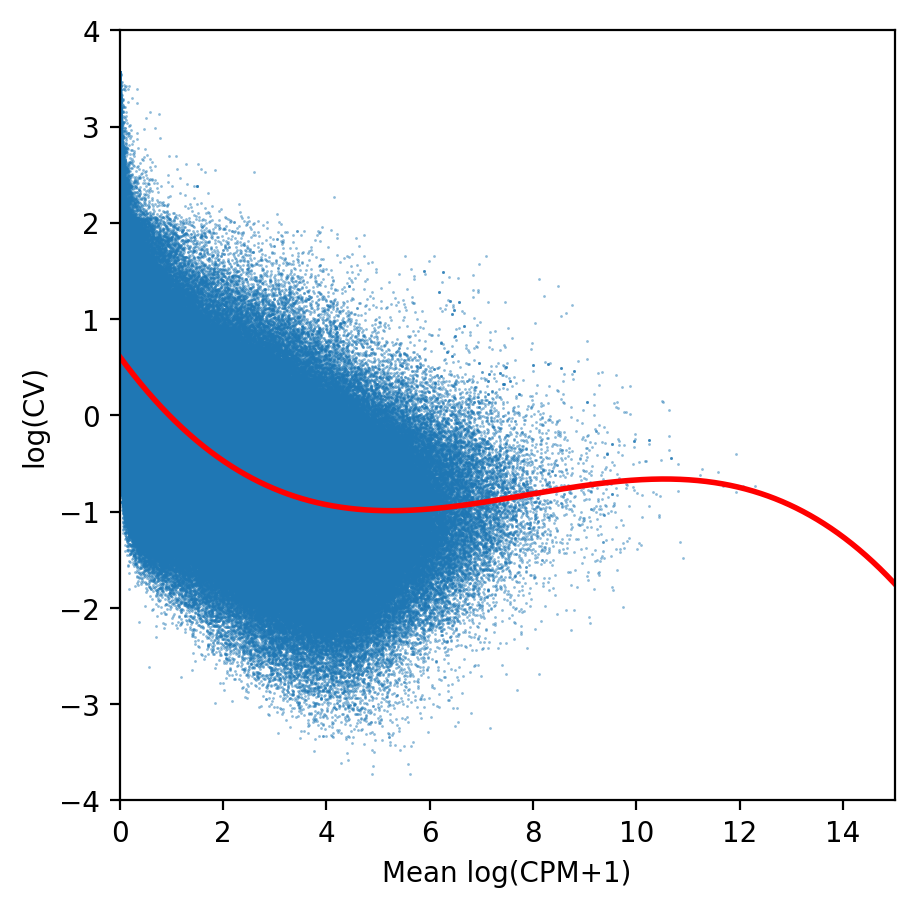
\includegraphics[width=9cm]{figures/mean_vs_coef_of_var.png}}
    \caption{\textbf{Fitting mean expression to coefficient of variation.} A scatterplot comparing mean log(CPM+1) expression values to the log of the coefficient of variation for the CPM expression values. We fit a univariate spline (red) to this data for use in the empirical Bayes-like estimation procedure of each gamma distribution's variance.}
    \label{fig:mean_vs_cv}
      \end{figure}
      
 \begin{figure}[htbp]
    \centerline{\includegraphics[width=13cm]{figures/empirical_bayes_results.pdf}}
    \caption{\textbf{Results applying empirical Bayes-like estimation approach.}  (a) Comparison between the distributions of average-precision generated by each method across all cell types.  (b) Comparison of the distributions over the highest achievable recalls when precision is fixed at 0.9 across all cell types. (c) Variants of the mean precision-recall curves for comparing the average performance of each method across all samples. (d) The joint-precision recall curves for all methods generating by ranking all sample-cell type output probabilities jointly.}
        \label{fig:shrinkage}
      \end{figure}
 
\end{appendices}
% \include{motivation/motivation}
% \include{related/related}

%% etc, etc.

%% Do you have appendices?  If so, add them here, just like chapters.
% \begin{appendices}
% \include{backmatter/appendix1}
% \end{appendices}

%% Are you a big nerd with a colophon?  Add it here.
%\begin{colophon}
%\svnidlong{$LastChangedBy$}{$LastChangedRevision$}{$LastChangedDate$}{$HeadURL: http://freevariable.com/dissertation/trunk/frontmatter.tex $}
\vcinfo{}

This template uses Gyre Pagella by default.  (I used Arno Pro in my dissertation.)

Feel free to give me a shout-out in your colophon or acks if this template is useful for you.  Good luck!

%\end{colophon}

%% McBride is a very nice style (some version is included in this distribution)
\bibliographystyle{mcbride}
\bibliography{the_master_bibliography}

%% Want an index?  Neither did I.
%\printindex

\end{document}
